% 経済工学Ⅰ 講義ノート(教科書版)
% コンパイル: lualatex main.tex (2回) または latexmk -lualatex main.tex
\documentclass[a4paper,11pt,book]{jlreq}

\usepackage{luatexja-fontspec}
\usepackage{amsmath,amssymb,amsthm}
\usepackage{mathtools}
\usepackage{bm}
\usepackage{booktabs}
\usepackage{array}
\usepackage{enumitem}
\usepackage{graphicx}
\usepackage{tikz}
\usetikzlibrary{arrows.meta,positioning,calc,decorations.pathreplacing}
\usepackage{pgfplots}
\pgfplotsset{compat=1.18}
\usepackage[most]{tcolorbox}
\usepackage[framemethod=TikZ]{mdframed}
\usepackage{hyperref}

% ============================================================
%  配色: 藍(primaryc)を基調に,要点=深緑,解答=琥珀 の3色で統一
% ============================================================
\definecolor{primaryc}{HTML}{2C3E70}
\definecolor{tealc}{HTML}{1F6F5C}
\definecolor{accentc}{HTML}{8A5A2B}

\hypersetup{colorlinks=true,linkcolor=primaryc,urlcolor=primaryc,
  pdftitle={経済工学I 講義ノート},pdfauthor={}}

% ---- リスト全体の見出しとの間隔(CJK環境では半角空白が詰まって
%      見えるため,ラベルと本文の間隔を確実な空きに置き換える) ----
\setlist[itemize,enumerate]{labelsep=0.7em, topsep=0.4em, itemsep=0.2em}
\setlist[description]{style=nextline, labelsep=0.7em,
  font=\bfseries\color{primaryc}, topsep=0.5em, itemsep=0.3em}

% ---- \paragraph を「同一行に回り込む」見出しでなく,独立した
%      見出し行に変更(見出し直後に文章が詰まって見える問題への対応) ----
\makeatletter
\renewcommand{\paragraph}[1]{%
  \par\vspace{0.9em}%
  {\normalfont\bfseries\color{primaryc!80!black}#1}%
  \par\vspace{0.35em}\nopagebreak}
\makeatother

% ---- 表の内部書式はデフォルトのまま(広げすぎない) ----

% ============================================================
%  定理環境系(定義・定理・命題・例・注意): mdframedで色枠に
% ============================================================
\mdfdefinestyle{boxedthm}{%
  linecolor=primaryc, linewidth=1pt,
  backgroundcolor=primaryc!5!white,
  roundcorner=4pt,
  innertopmargin=8pt, innerbottommargin=8pt,
  innerleftmargin=10pt, innerrightmargin=10pt,
  skipabove=16pt, skipbelow=16pt,
  splittopskip=10pt, splitbottomskip=6pt}
\mdfdefinestyle{lightaside}{%
  linecolor=primaryc!45!white, linewidth=2.4pt,
  leftline=true, rightline=false, topline=false, bottomline=false,
  backgroundcolor=primaryc!3!white,
  innertopmargin=6pt, innerbottommargin=6pt,
  innerleftmargin=10pt, innerrightmargin=8pt,
  skipabove=16pt, skipbelow=16pt}

\newtheoremstyle{boxedheadstyle}%
  {0pt}{0pt}{\normalfont}{0pt}%
  {\bfseries\color{primaryc}}{.}{.6em}%
  {\thmname{#1}\thmnumber{ #2}\thmnote{\ (#3)}}
\theoremstyle{boxedheadstyle}
\newmdtheoremenv[style=boxedthm]{definition}{定義}[chapter]
\newmdtheoremenv[style=boxedthm]{theorem}[definition]{定理}
\newmdtheoremenv[style=boxedthm]{proposition}[definition]{命題}

\newtheoremstyle{asideheadstyle}%
  {0pt}{0pt}{\normalfont}{0pt}%
  {\bfseries\color{primaryc!75!black}}{.}{.6em}%
  {\thmname{#1}\thmnumber{ #2}\thmnote{\ (#3)}}
\theoremstyle{asideheadstyle}
\newmdtheoremenv[style=lightaside]{example}[definition]{例}
\newmdtheoremenv[style=lightaside]{remark}[definition]{注意}

% ============================================================
%  読み物用ボックス: 要点(tealc) / 演習問題・解答(primaryc/accentc)
%  いずれも tcolorbox の「はみ出し見出し」で統一感を出す
% ============================================================
\newtcolorbox{keypoint}[1][要点]{%
  enhanced, breakable, colback=tealc!5!white, colframe=tealc!65!black,
  boxrule=0.8pt, arc=3pt,
  attach boxed title to top left={yshift=-2mm,xshift=4mm},
  boxed title style={colback=tealc!65!black, boxrule=0pt, arc=2pt,
    left=5pt, right=5pt, top=2pt, bottom=2pt},
  coltitle=white, fonttitle=\bfseries, title={#1},
  top=6mm, before skip=16pt, after skip=16pt}

\newtcolorbox{exercise}[1][演習問題]{%
  enhanced, breakable, colback=primaryc!4!white, colframe=primaryc!70!black,
  boxrule=0.8pt, arc=3pt,
  attach boxed title to top left={yshift=-2mm,xshift=4mm},
  boxed title style={colback=primaryc!70!black, boxrule=0pt, arc=2pt,
    left=5pt, right=5pt, top=2pt, bottom=2pt},
  coltitle=white, fonttitle=\bfseries, title={#1},
  top=6mm, before skip=16pt, after skip=4pt}

\newtcolorbox{answerbox}[1][解答と解説]{%
  enhanced, breakable, colback=accentc!5!white, colframe=accentc!75!black,
  boxrule=0.8pt, arc=3pt,
  attach boxed title to top left={yshift=-2mm,xshift=4mm},
  boxed title style={colback=accentc!75!black, boxrule=0pt, arc=2pt,
    left=5pt, right=5pt, top=2pt, bottom=2pt},
  coltitle=white, fonttitle=\bfseries, title={#1},
  top=6mm, before skip=4pt, after skip=16pt}

% ---- 数式マクロ ----
\newcommand{\E}{\mathrm{E}}
\newcommand{\Var}{\mathrm{Var}}
\newcommand{\Cov}{\mathrm{Cov}}
\newcommand{\Corr}{\mathrm{Corr}}
\newcommand{\dd}{\mathrm{d}}
\DeclareMathOperator*{\argmax}{arg\,max}
\DeclareMathOperator*{\argmin}{arg\,min}

\title{\Huge 経済工学Ⅰ 講義ノート\\[1ex]\Large ---金融工学入門---}
\author{講義:室町 幸雄(東京都立大学 経済経営学部)\\LaTeX編集版}
\date{2026年度 Sセメスター}

\begin{document}
\frontmatter
\maketitle

\chapter*{まえがき}
本書は,2026年度に東京大学工学部で開講された「経済工学Ⅰ」(担当:室町幸雄
先生,東京都立大学経済経営学部)の講義資料(全12回)および演習問題・解答を,
体系的な教科書の形に再構成したものである.原資料はスライド形式であったため,
箇条書きの内容を文章として書き下し,数式の導出過程や演習問題の考え方を含む
解説を補った.内容の取捨選択は原則として行っておらず,講義で扱われた事項は
すべて収録することを目指した.

各章は講義1回分に対応する.章末には当該回の演習問題とその解答・解説を収録した.

\tableofcontents

\mainmatter
% 第1章 金融取引と金融市場(資料1)
\chapter{金融取引と金融市場}

本章では，本講義全体の出発点として，金融 (finance) とは何か，経済主体はどのように
資金を調達するのか，そして証券市場 (securities market) がどのような役割を果たして
いるのかを概観する。数理的な議論は次章から始まるが，そこで扱う債券・株式などの
金融商品や市場の仕組みを，まずことばとして正確に理解しておくことが本章の目的である。

\section{金融}

\subsection{金融とは何か}

\begin{definition}[金融]
\textbf{金融}とは，余剰資金のある経済主体 A から，資金の不足している経済主体 B へ
お金を融通することをいう。
\end{definition}

このとき，資金を出す側の A を\textbf{貸し手}，資金を受け取る側の B を\textbf{借り手}と
呼ぶ。A の側から見ればこの行為は\textbf{投資}であり，B の側から見れば\textbf{調達}である。
すなわち，同じ資金の流れを，貸し手の視点で見るか借り手の視点で見るかによって
呼び方が変わる。

用語をいくつか整理しておく。貸し借りされるお金の本体を\textbf{元本}という。
元本の使用の対価として，借り手が支払うお金を\textbf{利子}，貸し手が受け取るお金を
\textbf{利息}と呼び分けることがある(講義では厳密には区別しないが，このような
使い分けがあることは知っておくとよい)。

\subsection{直接金融と間接金融}

資金の融通のされ方には，\textbf{直接金融}と\textbf{間接金融}の2つの形態がある。
両者の違いは，仲介者がどのような立場で取引に関与するかにある。

\begin{itemize}
\item \textbf{直接金融}：経済主体 A が，証券会社等の仲介者を通して，経済主体 B に
\emph{直接}資金を貸す形態。元本は A から B へ渡り，利子は B から A へ支払われる。
仲介者(証券会社等)は取引を仲介するだけであり，その対価として B から
\textbf{手数料}を受け取る。
\item \textbf{間接金融}：経済主体 A がまず仲介者(銀行等)に資金を預け，仲介者が
自らの名義で経済主体 B に貸し出す形態。元本は A $\to$ 銀行 $\to$ B と流れ，
利子は B が銀行に利率 $g$ で支払い，銀行は A に利率 $f$ で支払う。ここで
$f < g$ であり，その差(利鞘)が銀行の収益となる。
\end{itemize}

\begin{figure}[htbp]
\centering
\begin{tikzpicture}[
  box/.style={draw, rectangle, minimum width=2.4cm, minimum height=1.0cm, align=center},
  arr/.style={-{Stealth}, thick},
  node distance=3.2cm]
% 直接金融
\node[box] (A1) {経済主体\\A};
\node[box, right=of A1] (M1) {仲介者\\(証券会社等)};
\node[box, right=of M1] (B1) {経済主体\\B};
\draw[arr, red!70!black] ([yshift=2mm]A1.east) -- ([yshift=2mm]B1.west)
  node[pos=0.75, above]{元本};
\draw[arr, red!70!black] ([yshift=-2mm]B1.west) -- ([yshift=-2mm]A1.east)
  node[pos=0.75, below=1mm]{利子(利息)};
\draw[arr, blue!70!black] ([yshift=-4mm]B1.west) -- ([yshift=-4mm]M1.east)
  node[pos=0.5, below]{手数料};
\node[above=1mm of M1.north] {\textbf{直接金融}};
\end{tikzpicture}

\vspace{6mm}

\begin{tikzpicture}[
  box/.style={draw, rectangle, minimum width=2.4cm, minimum height=1.0cm, align=center},
  arr/.style={-{Stealth}, thick},
  node distance=3.2cm]
% 間接金融
\node[box] (A2) {経済主体\\A};
\node[box, right=of A2] (M2) {仲介者\\(銀行等)};
\node[box, right=of M2] (B2) {経済主体\\B};
\draw[arr, red!70!black] ([yshift=2mm]A2.east) -- ([yshift=2mm]M2.west)
  node[pos=0.5, above]{元本};
\draw[arr, red!70!black] ([yshift=-2mm]M2.west) -- ([yshift=-2mm]A2.east)
  node[pos=0.5, below]{利子(利息) $f$};
\draw[arr, red!70!black] ([yshift=2mm]M2.east) -- ([yshift=2mm]B2.west)
  node[pos=0.5, above]{元本};
\draw[arr, red!70!black] ([yshift=-2mm]B2.west) -- ([yshift=-2mm]M2.east)
  node[pos=0.5, below]{利子(利息) $g$};
\node[above=1mm of M2.north] {\textbf{間接金融}};
\node[below=5mm of M2.south, blue!70!black] {$f < g$};
\end{tikzpicture}
\caption{直接金融と間接金融における資金の流れ。直接と間接では，元本と利子の
「起点と終点」が異なることに注意する。}
\label{fig:direct-indirect}
\end{figure}

図\ref{fig:direct-indirect}のとおり，直接金融では元本・利子の流れの起点と終点は
A と B であるのに対し，間接金融ではいったん銀行を経由するため，A と B の間に
直接の貸借関係はない。この違いは，借り手が返済不能になったときに誰が損失を
被るかという点で決定的に重要である。

\begin{keypoint}[借り手 B が資金繰りに行き詰まったら?]
\begin{itemize}
\item \textbf{直接金融の場合}：貸しているのは経済主体 A 自身なので，損失を被るのは
A である。仲介者である証券会社は原則として損失を負わない。
\item \textbf{間接金融の場合}：B に貸しているのは銀行なので，まず損失を被るのは
銀行である。A は銀行に預金しているだけなので，銀行が健全である限り A の資金は
守られる。
\end{itemize}
つまり，直接金融では投資家がリスクを直接負担し，間接金融では銀行がリスクを
吸収する構造になっている。間接金融で $f<g$ という利鞘が存在するのは，銀行が
このリスク負担と仲介機能の対価を得ているためと解釈できる。
\end{keypoint}

\subsection{投資家，金融機関，事業会社}

金融取引に登場する経済主体は，次のように分類できる。

\begin{description}
\item[投資家] お金を融通する側の経済主体。
  \begin{itemize}
  \item \textbf{個人投資家}：個人としてお金を融通している経済主体。
  \item \textbf{機関投資家}：企業としてお金を融通している経済主体。顧客から集めた
  資金を運用・管理する法人投資家であり，保険会社，投資信託会社，信託銀行，
  年金基金，投資顧問会社，ヘッジファンドなどが該当する。
  \end{itemize}
\item[金融機関] 金融の仲介を業とする主体。
  \begin{itemize}
  \item \textbf{証券会社}：直接金融を営む金融機関。
  \item 間接金融を営む金融機関は多数ある。例として，普通銀行，郵便貯金銀行，
  信託銀行，信用金庫，信用協同組合などが挙げられる。
  \end{itemize}
\item[(一般)事業会社] 金融業以外の一般の企業。通常はお金の借り手側に立つ。
\end{description}

\section{資金調達}

事業会社が資金を調達する手段は，直接金融によるもの(有価証券の発行)と
間接金融によるもの(銀行借入)に大別される。

\subsection{直接金融における資金調達：有価証券}

直接金融では，証券会社を通して\textbf{有価証券}を取引することで資金のやり取りが
行われる。

\begin{definition}[有価証券]
\textbf{有価証券}とは，財産権を表章したものであり，それに記載された権利の行使や
移転(譲渡)がその証券によって行われるものをいう。
\end{definition}

有価証券は\textbf{債券}と\textbf{株券}に大別される。両者は資金調達者の貸借対照表上の
位置づけがまったく異なる。

\begin{itemize}
\item 債券で調達される資金は\textbf{負債}に該当する。負債とは返済義務のある契約，
すなわち借りているお金のことである。
\item 株券で調達される資金は\textbf{株式}と呼ばれ，自己資本に相当する。
\end{itemize}

以下で見るように，債券と株式は性質が大きく異なる。

\subsubsection{債券}

\begin{definition}[債券]
\textbf{債券} (bond) とは，資金調達を行う発行者(\textbf{発行体})が，お金を借りた
証拠として，利息の支払いや元本の返済を約束して発行する証書である。
\end{definition}

債券の保有者が受け取る将来のキャッシュフローは，\emph{ある程度は確定的}である。
すなわち，決まった日に決まった金額を受け取る(ただし発行体の破綻などの例外は
ある)。この「キャッシュフローの確定性」が，次章以降で債券を数理的に扱う際の
出発点となる。

債券に関する基本用語を整理する。
\begin{itemize}
\item \textbf{債権者}：お金を貸している側，すなわち投資家。
\item \textbf{債務者}：お金を借りている側，すなわち発行体。
\item \textbf{額面}：償還時に返済される元本の金額。
\item \textbf{利払い(クーポン)}：定期的に支払われる利息。
\item \textbf{償還日}：元本が返済される日(満期)。
\item \textbf{利払日}：クーポンが支払われる日。
\item \textbf{クーポンレート}：額面に対するクーポンの割合(年率で表示)。
\end{itemize}
日本では通常，クーポンは年2回払い，固定利率で，額面は1億円単位である。

\subsubsection{株式}

株式は債券とは対照的な性質をもつ。

\begin{itemize}
\item 投資家への\textbf{返済義務なし}，\textbf{満期なし}，\textbf{確定的な利払なし}。
\item 株式は自己資本に相当するので，\textbf{株主は当該事業会社の所有者}である。
\item 株主が受け取るお金はクーポンではなく\textbf{配当}である。配当金は業績次第で
決まり，業績によっては無配当になることもある。
\end{itemize}

株式投資家の将来キャッシュフローについては次の点が重要である。
\begin{itemize}
\item 投資の狙いは，\textbf{配当}と，\textbf{キャピタルゲイン}($\approx$ 売買益)を
得ることである。
\item 配当は定額ではなく，受け取れないこともあるため，不確実性が高い。
\item その結果，債券に比べると，株式の価値の変動性は相対的に高い。
\end{itemize}

また，株主は「会社の所有者」であるから，株主総会への参加権と議決権をもつ。
会社経営は経営陣が行うが，重要案件は株主総会を通す必要がある。議決権は株式の
保有枚数に応じて与えられるため，大株主ほど強い発言力をもつ。

\subsection{間接金融における資金調達：銀行借入}

\textbf{銀行借入}は間接金融による資金調達手段である。銀行借入による資金は，
事業会社にとって\textbf{負債}に該当する。この点で債券に似ている(資金調達者である
事業会社にとって，どちらも負債である)が，間接金融であることに注意が必要である。
本講義では，間接金融の貸し手を総じて\textbf{銀行}と呼ぶことにする。

\begin{itemize}
\item \textbf{融資}：銀行が事業会社に資金を貸すこと。
\item 用語：債権者(銀行)，債務者(事業会社)，元本，利払い，満期日，利払日，利率。
\end{itemize}

\subsubsection{預金：銀行の資金調達}

銀行が貸し出す資金は，投資家(預金者)から集めたものである。

\begin{itemize}
\item \textbf{預金}：投資家が銀行に貸し出した資金。特に，ゆうちょ銀行への預金は
\textbf{貯金}という。
\item \textbf{定期性預金}：満期がある預金。満期前に口座から引き出すと，ペナルティー
(預入期間の利息の減額)が科せられる。
\item \textbf{普通預金}：満期がなく，いつでも口座から引き出せる預金
(\textbf{要求払預金}とも呼ばれる)。
\end{itemize}

利率の大小関係について，次の点を押さえておく。事業会社への融資の利率に比べると，
預金の利率はかなり低い。さらに，普通預金の利率は定期性預金の利率よりも低い。
いつでも引き出せるという流動性の高さの代償として，利率が低くなっていると
解釈できる。なお，要求払預金には利息のつくものとつかないものがあり，事業会社の
決済用の\textbf{当座預金}には利息がつかない。

\section{証券市場}

\subsection{探索コストの低減}

金融取引は，余剰資金を貸したい人と，不足資金を借りたい人が\emph{出会わなければ}
成立しない。もし，貸したい人が借りたい人を探索するコスト，あるいは借りたい人が
貸したい人を探索するコストが非常に高かったら，金融取引はほとんど成立せず，
経済活動は大きく阻害されるだろう。したがって，\textbf{探索コストが低いことは，
経済全体にとって重要}である。

\begin{keypoint}[市場と銀行の役割]
直接金融において探索コストを低減し，取引を活発にする役割を果たしているのが
\textbf{証券市場}である。間接金融において同様の役割を果たしているのが
\textbf{銀行}である。
\end{keypoint}

\subsection{証券市場の形態}

\textbf{証券市場}とは，証券を取引する「場所」と考える(ただし実空間上の場所とは
限らない)。取引の形態には，取引所を通す取引と通さない取引がある。

\begin{description}
\item[取引所取引] 日本の(証券)取引所は，東京，大阪，名古屋，札幌，福岡にある。
取引所では定型化された商品(株式，債券など)が取引される。すべての商品を限られた
場所で取り扱うことはできないので，定型化された商品を，大きな取引量で，集中的に
捌くのが取引所の役割である。
\item[店頭取引(店頭市場)] 取引所を通さない取引(市場)。相対取引を軸に，
定型化されていないさまざまな商品，オーダーメイド商品などが取引されている。
\end{description}

市場は取引対象によって，債券市場，株式市場，オプション市場，スワップ市場，
などと呼び分けられる。

\subsection{債券市場}

証券市場は，新規に証券が発行される\textbf{発行市場} (primary market) と，
既に発行された証券が投資家間で売買される\textbf{流通市場} (secondary market) に
分けられる。

債券は，発行体，償還日，クーポンレートなど，何かしらの属性が異なれば別の銘柄と
なるため，\textbf{非常に多くの銘柄}が存在する。

\begin{description}
\item[発行市場] 債券を発行する市場。発行額の規模は，長期国債で1銘柄あたり数兆円，
国債全体では年間約200兆円に達する。通常，額面と(発行)価格は異なり，価格は
額面100円に対する価格で表示される。額面と価格が等しい場合を\textbf{パー} (par) と
いい，パーで発行することを\textbf{パー発行}という。額面より価格が高い場合を
\textbf{オーバーパー}，額面より価格が低い場合を\textbf{アンダーパー}という。
\item[流通市場] 既発債を取引する市場。債券の多くは店頭で取引されるため，実際の
市場価格はつかみにくい。そこで，マーケットメイカーによる売り気配・買い気配の
提示が行われている。価格情報としては，日本証券業協会の売買参考統計値や，
野村證券の JS-Price が有名である。
\end{description}

講義資料では，日本証券業協会のデータに基づく債券の年間発行額の推移が示された。
1998年から2024年頃までの間，債券の年間発行額の合計はおおむね150〜250兆円台の
規模で推移し，その大部分を国債が占める。普通社債の発行額はそれよりはるかに
小さく，年間10〜20兆円程度の規模である。

\subsection{株式市場}

債券と違い，株式では既存の株券も追加発行の株券も同じ扱いであり，ある会社の
株式の価格(\textbf{株価})は1つである。株価は会社の価値を反映するものと
考えられる。

\begin{definition}[株式時価総額]
\[
\text{株式時価総額} = \text{株価} \times \text{発行済株式数}.
\]
\end{definition}

講義資料に示された日本の株式時価総額の実績値を挙げると，東証一部で709兆円・
東証全体で730兆円(2022年3月末)，プライム市場で684兆円・東証全体で712兆円
(2022年4月末)，プライムで970兆円・東証全体で1,008兆円(2024年3月末)，
プライムで911兆円・東証全体で947兆円(2025年3月末)，プライムで1,327兆円・
東証全体で1,372兆円(2026年2月末)となっている。長期の推移を見ると，
1980年代末のバブル期に約600兆円まで拡大した後に崩壊し，2000年代以降は
変動を伴いながら拡大して，近年は1,000兆円を超える規模に達している。

\subsubsection{東証の市場区分変更}

2022年4月4日，東京証券取引所の市場区分が変更された。従来の
「東証1部」「東証2部」「マザーズ」「ジャスダック」から，
「\textbf{プライム}」「\textbf{スタンダード}」「\textbf{グロース}」へ再編された。

変更の背景は次の2点である。
\begin{enumerate}
\item 市場区分のコンセプトの明確化。
\item 持続的な企業価値向上の動機付けとなる仕組み作り。
\end{enumerate}

新しい各市場区分のコンセプトは以下のとおりである。
\begin{itemize}
\item \textbf{プライム}：高い流動性と高いガバナンス水準(の企業向け)。
\item \textbf{スタンダード}：一定の流動性と基本的なガバナンス水準。
\item \textbf{グロース}：高い成長可能性をもつが，相対的にリスクは高い。
\end{itemize}

この市場区分変更に伴い，株価指数(TOPIX等)の算出方法も変更されている。

\subsection{流動性と証券化}

債券市場や株式市場は，証券に\textbf{流動性}を供給している。

\begin{definition}[流動性]
売買したいときに，適正な価格付近で，すぐに売買できるとき，\textbf{流動性が高い}
という。逆の状態を\textbf{流動性が低い}という。
\end{definition}

一方，銀行の個々の融資は市場で取引されない。すなわち流動性はない。仮に取引が
あっても外からは見えない(透明性を高める努力もあったが，十分ではない)。

\begin{definition}[証券化]
\textbf{証券化}とは，流動性のない資産を市場で売買できるようにする仕組みの一つ
である。多くの非流動性資産(ここでは融資)を集め，そこから生じるキャッシュ
フローをもとに，新たなリスク・リターン特性をもつ証券を組成し，販売する。
\end{definition}

2008年前後の金融危機で「活躍」したのは，住宅ローンの証券化商品である
RMBS (Residential Mortgage Backed Securities) である。さらに，
CDO (Collateralized Debt Obligations) や，合成CDOの素になる
CDS (Credit Default Swap) も金融危機において重要な役割を果たした。

\section*{参考：MBO(マネジメント・バイアウト)}

\textbf{マネジメント・バイアウト} (Management Buyout; MBO) とは，経営陣が自ら
株式を取得して株主になることをいう。自分達の経営戦略を円滑に進められるように
するための手法の一つであり，次のような場面で使われる。

\begin{itemize}
\item 経営陣による会社の買収(自己所有化)。
\item 企業グループ内の会社が，グループから分離独立するとき。
\item 他社による買収への対抗策。
\end{itemize}

上場企業が\textbf{敵対的買収}(買収者が，買収対象会社の取締役会の同意を得ないで
買収を仕掛けること)を回避するため，経営陣が MBO を行って市場から株式を
買い集め，上場を廃止して非公開会社にする，といったケースもある。

% 第2章 キャッシュフローと時間価値(資料2)
\chapter{キャッシュフローと時間価値}

本章から数理的な議論に入る。鍵となる概念は「お金の価値は受け取る時点によって
異なる」という\textbf{時間価値} (time value) の考え方である。将来のキャッシュ
フローが確定的な場合に，ある時点のキャッシュフローを(経済学的に等価な)異なる
時点のキャッシュフローに変換する方法---現在から将来へ，将来から現在へ---を学び，
その応用として投資の価値評価法(NPV法・IRR法)を扱う。題材としては，キャッシュ
フローが単純で有価証券の代表例である債券を用いる。

\section{債券}

\subsection{債券のキーワード}

債券の特性を示すキーワードとして，以下を押さえておく。

\begin{itemize}
\item \textbf{額面} (face value)：償還時に返済される金額。
\item \textbf{満期} (maturity)：元本が償還される時点。
\item \textbf{券面利率}(クーポンレート，coupon rate)：利息計算に使われる利率。
これに基づいて支払われる利札を\textbf{クーポン} (coupon) という。
\item \textbf{利払頻度}：年払い，半年払いなど。
\item \textbf{発行体} (issuer)：債券を発行して資金を調達する主体。
\item \textbf{信用格付け} (credit rating)：発行体の信用力の評価。
\end{itemize}

\subsection{キャッシュフローによる分類}

\begin{description}
\item[利付債] 満期まで定期的に利払が行われる債券。満期に額面分が償還されることを
\textbf{満期一括償還}という。満期一括償還債では，満期に利払額と償還額の合計額が
支払われる。
\item[割引債] 利払がなく，満期に額面分の金額が償還される債券。
\end{description}
なお，上記に該当しない，元本を分割して償還するアモチ型の債券もある。

その他の分類として，
\begin{itemize}
\item \textbf{有期債}(満期のあるもの)と\textbf{永久債}(満期のないもの)，
\item \textbf{固定利付債}(券面利率が一定)と\textbf{変動利付債}(券面利率が変動する)，
\end{itemize}
がある。

\subsection{発行体による分類}

\begin{description}
\item[国債] 国が発行している債券。発行額も発行頻度も高く，知名度は債券で
No.~1。多くは金融機関や機関投資家向けだが，個人向けの国債もある。
\item[政府保証債] 政府関係機関や特殊法人が発行する債券で，政府による支払保証が
ついているもの。
\item[地方債] 地方公共団体が発行している債券。
\item[社債] 一般事業会社が発行している債券。いろいろな種類と条件のものがある。
\item[電力債] 各地方の電力会社が発行している債券。発行額が大きい。
\end{description}

\subsection{キャッシュフローの図示}

キャッシュフロー(以下 CF と略すことがある)の作図には次の約束を設ける。
時刻を横軸にとり，キャッシュフローは発生時刻上の縦方向の矢印で示す。
\textbf{正(受取)は上向き，負(支払)は下向き}である。縦のスケールを正確に
書くとわかりにくい場合は，適当に歪めて書いてよい。

\subsection{固定利付債のキャッシュフロー}

固定利付債のキャッシュフローを定式化する。
\begin{itemize}
\item 利払日：$t_i$ ($i=1,2,\dots,m$;\ $t_m$：満期，$t_0=0$)。時刻は年単位で表す。
\item 額面：$F$。
\item クーポンレート：$K$(\emph{必ず年率で表示})。
\item クーポン：
\begin{equation}
C_i = K \times F \times (t_i - t_{i-1}).
\label{eq:coupon}
\end{equation}
\end{itemize}
式\eqref{eq:coupon}は，「年率 $K$ の利息が，期間 $(t_i-t_{i-1})$ 年分だけ額面 $F$ に
対して付く」ことを表している。期間 $(t_i - t_{i-1})$ も年単位で表示することに注意。

\begin{figure}[htbp]
\centering
\begin{tikzpicture}[scale=1.1]
\draw[-{Stealth}] (0,0) -- (9.5,0) node[right]{$t$};
\fill (0,0) circle (1.5pt) node[below=1mm]{$0$};
\foreach \x/\lab in {1.5/t_1, 3/t_2, 5.5/t_i, 7.5/t_m}{
  \node[below] at (\x,-0.05) {$\lab$};}
\draw[-{Stealth}, thick] (1.5,0) -- (1.5,0.8) node[above]{$C_1$};
\draw[-{Stealth}, thick] (3,0) -- (3,0.8) node[above]{$C_2$};
\node at (4.2,0.5) {$\cdots$};
\draw[-{Stealth}, thick] (5.5,0) -- (5.5,0.8) node[above]{$C_i$};
\node at (6.5,0.5) {$\cdots$};
\draw[-{Stealth}, thick] (7.4,0) -- (7.4,0.8) node[above]{$C_m$};
\draw[-{Stealth}, very thick] (7.6,0) -- (7.6,2.0) node[above]{$F$};
\end{tikzpicture}
\caption{固定利付債のキャッシュフロー。満期 $t_m$ にはクーポン $C_m$ に加えて
額面 $F$ が償還される。}
\label{fig:fixedbond-cf}
\end{figure}

\begin{example}[固定利付債のキャッシュフロー]
満期2年，年2回払，クーポンレート4\%，額面100円の固定利付債を考える。
利払日は $t_i = i/2$ 年($i=1,2,3,4$;満期2年)であり，クーポンは
式\eqref{eq:coupon}より
\[
C_i = 4\% \times 100 \times 0.5 = 2 \text{ 円}
\]
となる。すなわち，0.5年後，1年後，1.5年後に2円ずつ，2年後にクーポン2円と
額面100円の合計102円を受け取る。
\end{example}

\begin{example}[割引債のキャッシュフロー]
満期2年，額面100円の割引債を考える。利払はなく，キャッシュフローは満期日
(2年後)の100円のみである。
\end{example}

\vspace{18pt}

\subsection{変動利付債のキャッシュフロー}

変動利付債では，クーポンレートが市場金利に連動して変動する。従来の標準物では
クーポンレートとして 6M-LIBOR(6ヶ月物LIBOR金利)$L_{i-1}$ が使われ，クーポンは
\begin{equation}
C_i = F \, L_{i-1} (t_i - t_{i-1})
\end{equation}
で与えられた。ここで重要なのは添字が $i-1$ であることである。すなわち，標準物では
クーポンレートは\emph{前回の利払日} $t_{i-1}$ に決まり，利払日 $t_i$ の利息額は
前回の利払日 $t_{i-1}$ の時点で確定する。これは「借りる時に利子は既知」という
原則に沿ったものである。

\begin{remark}[LIBORの廃止と後決め金利]
2021年末，LIBORは代表的な変動金利ではなくなった。現在の変動利付債では，日々の
「当日から翌日までの金利」(オーバーナイト金利，ON金利)による複利運用の
一定期間分の成果をまとめて払う方式が使われている。

例として，今から半年後の利息額を考える。$t$ 日目のオーバーナイト金利 $r_t$ は
その当日に確定する。$t$ 日目の1円は，$t+1$ 日には $1 + r_t \Delta t$ 円になる
($\Delta t$:1日の年換算値)。これを半年分積み重ねる(=掛け続ける)と，
半年後には
\[
(1 + r_0 \Delta t)(1 + r_1 \Delta t) \cdots (1 + r_{\text{半年後}-1} \Delta t)
\]
となり，半年前の1円との差(=半年間で増えた分)
\[
(1 + r_0 \Delta t)(1 + r_1 \Delta t) \cdots (1 + r_{\text{半年後}-1} \Delta t) - 1
\]
が利息額になる。この利息額が確定するのは，$t=0$ ではなく
$t = \text{半年後} - \Delta t$ の時点である。

このように，従来の変動金利は\textbf{先決め金利}(今回の利払日の利息額は前回の
利払日に確定)であったのに対し，現在の変動金利は\textbf{後決め金利}(今回の
利払日の利息額は今回の利払日の直前に確定)である。これによって，金利デリバティブに
よっては評価方法が変更されたものもある。
\end{remark}

\vspace{18pt}

\section{時間，価値，利回り}

本節では，将来が確定的な場合を考え，ある時点の CF を(経済学的に等価な)異なる
時点の CF に変換する方法を学ぶ。

\subsection{現在価値の考え方}

将来のキャッシュフローが確定している場合を考える(確定的でない場合を扱うのが，
本講義後半のデリバティブの価格付け理論である)。

1円投資したとき，1年後に $(1+R)$ 円が確実に返ってくる場合を考える。1円は元本，
$R$ 円は利息(利子)である。このとき，\textbf{1年後の1円の現在価値(現時点に
おける価値)} $D(1)$ はいくらだろうか(記号 $D(1)$ の $1$ は「1年後」の意味)。

これは比例計算で算出できる：
\[
\begin{array}{ccc}
1 \text{ 円} & \longrightarrow & 1+R \text{ 円}\\
D(1) \text{ 円} & \longrightarrow & 1 \text{ 円}
\end{array}
\qquad\Longrightarrow\qquad
D(1) = \frac{1}{1+R}.
\]
左側の金額を\textbf{現価(現在価値)}，右側の金額を\textbf{終価}と呼ぶ。

\subsection{利回り}

\begin{definition}[利回り]
\textbf{利回り}とは，単位時間あたりの平均利子率である。利回りは年率(単位時間は
1年)で表示するのが原則である。
\end{definition}

利回りにはいろいろな考え方があり，一番大きなポイントは\textbf{利息を再投資するか
否か}である。また，年あたりの再投資回数を\textbf{転化回数}という。

\subsection{再投資と現在価値}

前述の例は1年を1期間として考えたケースであった。では，半年ごとに再投資が可能
(転化回数 $m=2$)だとしたらどうなるか。半年を1期間とみなせば，1年間は2期間に
なる。ここで注意すべきは，\emph{利率 $R$ は年率で定義されている}という約束事で
ある。$m=2$ のときの1期間は半年であり，その間に増えるのは比率 $R/2$ である。
したがって比例計算により
\[
\begin{array}{ccccc}
1 \text{ 円} & \to & 1+R/2 \text{ 円} & \to & (1+R/2)^2 \text{ 円}\\
D(1) \text{ 円} & \to & & \to & 1 \text{ 円}
\end{array}
\qquad\Longrightarrow\qquad
D(1) = \frac{1}{(1+R/2)^2}.
\]
一般に，転化回数 $m$(=$1/m$ 年ごとに再投資が可能)ならば，
\begin{equation}
1 \text{ 円} \to \cdots \to \Bigl(1+\frac{R}{m}\Bigr)^m \text{ 円},
\qquad
D(1) = \frac{1}{(1+R/m)^m}.
\label{eq:D1m}
\end{equation}

\subsection{利息を再投資しない場合とする場合}

\paragraph{利息を再投資しない場合。}
利息をその後の投資にまわさず，回収する場合を考える。1回の投資期間が半年
($1/2$年)ならば，1年で投資を2回繰り返す。年間の利息は，1回の投資期間(半年)で
得られる利息の2倍になる(ただし，1回の投資期間で得られる利息は年率の $1/2$)。
すなわち，元本1円に対して1年で得られる利息は
\[
\frac{R}{2} \times 2 = R \text{ 円}.
\]
同様に，1回の投資期間が3ヶ月($1/4$年)ならば1年で投資を4回繰り返し，年間の
利息は $\frac{R}{4}\times 4 = R$ 円となる。つまり，再投資しなければ，転化回数に
よらず年間の利息は $R$ 円である。

\paragraph{利息を再投資する場合。}
利息全額をその後の投資にまわす場合を考える。1回の投資期間が半年ならば，1年後の
総価値は1回の投資(半年)で得られる価値の2乗となる：
\[
1 \text{ 円} \to 1 + \frac{R}{2} \text{ 円} \to \Bigl(1+\frac{R}{2}\Bigr)^2 \text{ 円}.
\]
1年で得られる利息は $(1+R/2)^2 - 1$ 円である。1回の投資期間が3ヶ月ならば，
1年後の総価値は $(1+R/4)^4$ 円になる。

\subsection{単利と複利}

利回りには，\textbf{単利}と\textbf{複利}がある。

\begin{description}
\item[単利] 利子を再投資\emph{しない}で得られる利回り。一般に，単利の利回りは
\[
\text{(単利利回り)} = \frac{\text{(受取金額)}-\text{(支払金額)}}
{\text{(支払金額)}\times\text{(期間)}}
\]
という形，すなわち「単位時間で，どのくらいの比率だけ増えたか」で計算される。
額面 $F$，クーポンレート $K$(年 $m$ 回払い)，満期 $T$ 年後の債券が，現在
$p$ 円で取引されているとすると，利回り(単利)は
\begin{equation}
\frac{\dfrac{1}{p}\Bigl(F + F \times \dfrac{K}{m}\times m \times T - p\Bigr)}{T}
= \frac{F-p}{pT} + \frac{FK}{p}
\end{equation}
となる。特に $K=0$(割引債)ならば $\dfrac{F-p}{pT}$，$F=p$(パー)ならば $K$ と
なる。なお，この単利利回りが，そのまま(複利の)利回り $R$ になるわけではない
ことに注意する。
\item[複利] 利子を全額再投資して得られる利回り。再投資の間隔により，1年複利，
半年複利，3ヶ月複利，…がある。投資の一期間の長さによって，同じ利回りでも終価は
異なる。
\end{description}

\subsection{複利による終価と現価}

複利の場合の1年後の関係を整理する。利子率を年率 $R$ とすると，
\begin{itemize}
\item 半年ごとに再投資($m=2$):$1$ 円 $\to (1+R/2)^2$ 円，
$D(1) = (1+R/2)^{-2}$。
\item $1/m$ 年ごとに再投資：$1$ 円 $\to (1+R/m)^m$ 円，
$D(1) = (1+R/m)^{-m}$。
\end{itemize}

\begin{example}[複利による終価]
利子率(年率)を10\%とする。1円投資したときの1年後の価値(円)は：
\begin{enumerate}
\item[(1)] 1年複利のとき，$1 + 0.1 = 1.1$。
\item[(2)] 半年複利のとき，$\bigl(1+\frac{0.1}{2}\bigr)^2 = 1.1025$。
\item[(3)] 3ヶ月複利のとき，$\bigl(1+\frac{0.1}{4}\bigr)^4 \approx 1.1038$。
\item[(4)] $1/m$ 年複利のとき，$\bigl(1+\frac{0.1}{m}\bigr)^m$。
\end{enumerate}
\end{example}

転化回数 $m$ を増やすと1年後の価値(終価)は増加するが，無限に上昇するわけでは
ない。次に見る\textbf{連続複利}が上限を与える。

\subsection{連続複利}

連続時間への極限，すなわち $1/m$ 年複利で $m \to \infty$ のケースを考える。
このときの1年後の価値は $\lim_{m\to\infty}(1+R/m)^m$ である。ここで，
ネイピア数 $e$ の定義
\[
e = \lim_{n\to\infty}\Bigl(1 + \frac{1}{n}\Bigr)^n = 2.71828\cdots
\]
を用いる。$n = m/R$ と置き換えると，$m\to\infty$ のとき $n\to\infty$ であり，
\begin{equation}
\lim_{m\to\infty}\Bigl(1+\frac{R}{m}\Bigr)^{m}
= \lim_{m\to\infty}\Biggl[\Bigl(1+\frac{1}{m/R}\Bigr)^{m/R}\Biggr]^{R}
= e^{R}.
\end{equation}
$R = 10\%$ のとき $e^{0.1} \approx 1.1052$ であり，これが転化回数を増やしたときの
終価の上限である。

同様に，現価についても
\begin{equation}
D(1) = \lim_{m\to\infty}\Bigl(1+\frac{R}{m}\Bigr)^{-m}
= \lim_{m\to\infty}\Biggl[\Bigl(1+\frac{1}{m/R}\Bigr)^{m/R}\Biggr]^{-R}
= e^{-R}
\end{equation}
となる。

\subsection{整理：現価・終価・利回り}

\begin{keypoint}[現価・終価・利回りの考え方]
「現価」と「終価」は同じ考え方に基づいて計算される。
\begin{itemize}
\item \textbf{利回り}は，投資期間中の平均利子率を(年率で)表示した値。
\item \textbf{終価}は，利息も含めて得られる全額を常に再投資するとき，「初期投資額が，
ある将来時点で達する金額」。
\item \textbf{現価}は，利息も含めて得られる全額を常に再投資するとき，「ある将来時点で
ある金額を得るために必要な初期投資額」。
\end{itemize}
年 $m$ 回再投資可能で，利回り(年率)を $R$ とすると，
\[
\text{(1円の1年後の)終価:} \Bigl(1+\frac{R}{m}\Bigr)^{m},
\qquad
\text{(1年後の1円の)現価:} \Bigl(1+\frac{R}{m}\Bigr)^{-m}.
\]
\end{keypoint}

さらに，次の点に注意する。
\begin{itemize}
\item 現価と終価が等しくても，転化回数 $m$ が異なると，利回り $R$ は異なる値をとる。
\item 利回り $R$ が等しくても，転化回数 $m$ が異なると，現価や終価は異なる値をとる。
\item 利息(利子)も含めて全額再投資する考え方を「複利」といい，その考え方で
得られる利回り $R$ を「複利(利回り)」という($\Leftrightarrow$ 単利(利回り))。
\item 特に $m\to\infty$，つまり瞬間的に再投資を繰り返すことを「連続複利」，
そのときの複利利回りを「連続複利(利回り)」という。
\end{itemize}

\begin{example}[例題2-1]
複利利回り(年率)を5\%とする。
(1) いま100円投資したときの1年後の価値(終価)，
(2) 1年後の100円の現在価値(現価)，
を (A) 1年複利，(B) 半年複利，(C) 3ヶ月複利，(D) 連続複利，のそれぞれの場合に
ついて求めなさい。

\medskip
\noindent\textbf{解答。}
終価は $100\times(1+0.05/m)^m$，現価は $100\times(1+0.05/m)^{-m}$(連続複利では
それぞれ $100e^{0.05}$，$100e^{-0.05}$)で計算して，次表を得る。
\vspace{0.9em}
\begin{center}
\begin{tabular}{lcc}
\toprule
 & 終価 & 現価\\
\midrule
1年複利 & 105.000 & 95.238\\
半年複利 & 105.063 & 95.181\\
3ヶ月複利 & 105.095 & 95.152\\
連続複利 & 105.127 & 95.125\\
\bottomrule
\end{tabular}
\end{center}
\vspace{0.9em}
転化回数が増えるほど終価は大きく，現価は小さくなり，連続複利がその極限を与える
ことが確認できる。
\end{example}

\vspace{18pt}

\subsection{$n$ 年間の現価・終価}

複利利回り $R$，年 $m$ 回の再投資を考え，期間を $n$ 年に伸ばす。

\begin{itemize}
\item $m=1$ のとき：現在の1円の $n$ 年後の終価は $(1+R)^n$，$n$ 年後の1円の
現価は $(1+R)^{-n}$。
\item $m=2$ のとき：半年を1期間として $2n$ 期間あるので，終価は
$(1+R/2)^{2n}$，現価は $(1+R/2)^{-2n}$。
\item 一般に，転化回数 $m$ のとき：
\begin{equation}
\text{終価} = \Bigl(1+\frac{R}{m}\Bigr)^{mn},
\qquad
\text{現価} = \Bigl(1+\frac{R}{m}\Bigr)^{-mn}.
\label{eq:discrete-general}
\end{equation}
\end{itemize}
式\eqref{eq:discrete-general}が\textbf{離散時間モデルでの一般形}である。

連続複利利回り $R$ の場合は，$m\to\infty$ の極限をとって
\begin{equation}
\text{終価} = \lim_{m\to\infty}\Bigl(1+\frac{R}{m}\Bigr)^{mn} = e^{Rn},
\qquad
\text{現価} = \lim_{m\to\infty}\Bigl(1+\frac{R}{m}\Bigr)^{-mn} = e^{-Rn}
\label{eq:continuous-general}
\end{equation}
となる。式\eqref{eq:continuous-general}が\textbf{連続時間モデルでの一般形}である。

\section{確定的なキャッシュフローの価値}

\subsection{考え方：分解と線形和}

複数の将来キャッシュフローをもつ証券の価値は，次の原理で評価する。

\begin{keypoint}[価値評価の基本原理]
「全ての将来キャッシュフローを持つ証券」の価値
$=$「個々の将来キャッシュフローの価値」の総和。

なぜならば，経済価値はどちらも同じだからである。つまり，証券を一つ一つの
キャッシュフローに分解して評価し，合計すればよい。
\end{keypoint}

\begin{example}
先の固定利付債(満期2年，年2回払，クーポンレート4\%，額面100円)の価値は，
半年複利の利回り $R$(転化回数 $m=2$)を用いると
\[
V = \frac{100}{\bigl(1+\frac{R}{2}\bigr)^4}
+ \sum_{i=1}^{4}\frac{2}{\bigl(1+\frac{R}{2}\bigr)^{i}}
\]
となる。
\end{example}

一般に，時刻 $t_i$ のキャッシュフロー $C(t_i)$， $i=1,2,\dots,n$ をもつ証券の
価値は，転化回数を $m$ として
\begin{equation}
V = \sum_{i=1}^{n}\frac{C(t_i)}{\bigl(1+\frac{R}{m}\bigr)^{m t_i}}
\label{eq:value-general}
\end{equation}
である。

\subsection{現価，終価，複利利回りの関係}

キャッシュフローが1回の場合の現価と終価の関係，そして利回りを整理する。
$T$ を期間，$PV$ を現価，$FV$ を終価，$R$ を複利利回り，$m$ を転化回数とすると，
\begin{equation}
PV\Bigl(1+\frac{R}{m}\Bigr)^{mT} = FV,
\qquad\text{あるいは(連続複利で)}\quad
PV \cdot e^{RT} = FV.
\label{eq:pv-fv}
\end{equation}
これは「$[0,T]$ の期間中，どの時点も常に利回りは $R$ である」と考えることに
相当する(利回りの定義は期間平均収益率だからである)。個々のキャッシュフローに
対して式\eqref{eq:pv-fv}の関係が成立し，将来キャッシュフローが複数回のときは
価値を線形和で評価する。

\begin{example}[キャッシュフローが1回のケースの $R$]
$T$ 年後に $C$ 円のキャッシュフローがあり，その現在価値(現価)が $A$ 円だと
する。$PV = A$， $FV = C$ なので $A = C(1+R/m)^{-mT}$。これを $R$ について解くと
\begin{equation}
R = m\Biggl[\Bigl(\frac{C}{A}\Bigr)^{\frac{1}{mT}} - 1\Biggr].
\end{equation}
連続複利では $A = Ce^{-RT}$ より
\begin{equation}
R = \frac{1}{T}\log\frac{C}{A}.
\end{equation}
\end{example}

\begin{example}[キャッシュフローが複数回のケースの $R$]
$t_i$ 年後に $C_i$ 円のキャッシュフロー($i=1,2,\dots,n$)があり，現在価値
(現価)が $A$ 円だとする。このとき
\begin{equation}
A = \sum_{i=1}^{n}\frac{C_i}{(1+R/m)^{m t_i}},
\qquad\text{連続複利では}\quad
A = \sum_{i=1}^{n} C_i e^{-R t_i}
\end{equation}
が成り立つ。$A$ が既知のとき，この方程式の解 $R$ を「(債券の)複利利回り」と呼ぶ。
\end{example}

\vspace{18pt}

\subsection{これらは何をやっているのか}

これらの計算の本質は，\textbf{ある時点のキャッシュフローを，「経済学的に等価な」
別の時点のキャッシュフローに変換している}，ということである。現在の CF を将来の
CF に変換することもあれば，将来の CF を現在の CF に変換することもある。現在の
CF(の価値)が現価，最終時点(将来)の CF の価値が終価である。

特に，将来の CF を現在の CF に変換することを，将来の CF を\textbf{割り引く}
という。この割り引きに使われる利回りを\textbf{割引率}と呼ぶことがある。

\subsection*{閑話休題：72の法則}

あるTVドラマでも取り上げられたという「72の法則」を紹介する。

72の法則とは，投資した元本が2倍になるまでの年数を金利から計算する式
\[
\text{年数} = \frac{72}{\text{金利(\%)}}
\]
のことである。これは連続複利で説明できる。元本を $A$，金利を $r$，年数を $T$ と
すると，
\[
A e^{rT} = 2A
\]
より $rT = \log 2$。ゆえに
\[
T = \frac{\log 2}{r} \approx \frac{0.693}{r} = \frac{69.3}{r(\%)}
\approx \frac{72}{r(\%)}.
\]
厳密には「69.3の法則」だが，72は約数が多く暗算しやすいため72が使われている。
連続複利による厳密な値と72の法則による近似値を比べると，金利1\%のとき厳密には
約69.3年に対し72の法則では72年，金利10\%のとき厳密には約6.93年に対し7.2年，
といった具合で，実用上十分な近似になっている。

\section{投資の価値評価：将来CFが確定的な場合}

前節の考え方の応用として，投資プロジェクトの評価法を扱う。

\subsection{伝統的な投資評価法}

代表的な方法は次の2つである。
\begin{itemize}
\item \textbf{NPV法}(Net Present Value 法，正味現在価値法)
\item \textbf{IRR法}(Internal Rate of Return 法，内部収益率法)
\end{itemize}

より古い方法には\textbf{回収期間法}がある。これは，将来キャッシュフローを何期間分
累積すれば初期投資額を回収できるかを考え，その回収期間が短い方を選ぶ，という
考え方である。しかしこの方法には，キャッシュフローの時間価値が考慮されていない
という欠点があり，ファイナンス流の考え方ではない。

\subsection{NPV(正味現在価値)法}

\begin{definition}[NPV]
現在の投資に必要な資金を $CF(0)$，時点 $i$ における将来キャッシュフローを
$CF(i)$，割引率を $R$ とすると，
\begin{equation}
NPV = \sum_{i=1}^{N}\frac{CF(i)}{(1+R)^i} - CF(0).
\label{eq:npv}
\end{equation}
(注：1年を一期間として表現を単純化している。)
\end{definition}

基本的な考え方は，「$NPV > 0$ となる投資は将来の利益をもたらすことになるので，
合理的な投資である」と判断するものである。

ただし，NPV法には次の問題点がある。
\begin{itemize}
\item NPV の値は $R$ のとり方次第で変わる。$R$ としてどのような値が適切かが
問題になる。
\item 初期投資額が大きければ，NPV(の絶対値)は高くなりがちである
($CF(i)$ を定数倍にすると NPV も定数倍になる)。すなわち，NPV は投資の
\emph{効率性}の評価ではない。
\end{itemize}

\subsection{IRR(内部収益率)法}

\begin{definition}[IRR]
$NPV = 0$ を満たす割引率 $R$ を \textbf{IRR}(内部収益率)という。
\end{definition}

IRR法では，IRR を算出し，それが\textbf{資金調達コスト}よりも高ければ投資する
価値あり，と判断する。

\begin{itemize}
\item IRR は，投資を実行した場合の\emph{期間平均収益率}に相当する。したがって，
IRR がより高い商品に投資するのが良い，と考える。すなわちIRR法は投資の
\emph{効率性}を評価している。
\item 資金調達コストとは，企業が資金調達する際に要する内部収益率である。例えば
銀行借入による調達では，利子払等を考えて算出する。
\item 資金調達コストは調達手段(債券，株式，銀行借入等)により異なる。企業の
場合は，総合的な\textbf{加重平均資本コスト}(WACC)で考える。
\end{itemize}

\begin{definition}[加重平均資本コスト(WACC)]
自己資本額を $S$，負債額を $D$，株式コスト(要求利回り)を $R_S$，負債コスト
(要求利回り)を $R_D$ とする。自己資本比率を
\[
k = \frac{S}{S+D}
\]
とすると，加重平均資本コスト (Weighted Average Cost of Capital) は
\begin{equation}
WACC = \frac{S R_S + D R_D}{S+D} = k R_S + (1-k) R_D.
\end{equation}
\end{definition}

\vspace{18pt}

\subsection{IRR法とNPV法の関係}

NPV を割引率 $R$ の関数 $NPV(R)$ とみなすと，(将来CFがすべて正なら)
$NPV(R)$ は単調減少関数である。$NPV(R)=0$ となる点が IRR であり，
\[
\text{割引率} < IRR \;\Rightarrow\; NPV > 0,
\qquad
\text{割引率} > IRR \;\Rightarrow\; NPV < 0
\]
が成り立つ(単調性より逆向きの矢印も成立する)。企業の投資判断では，割引率として
WACC を用い，IRR と WACC の比較で考える。IRR $>$ WACC ならば $NPV(WACC)>0$ と
なり，投資は合理的と判断される。

\begin{figure}[htbp]
\centering
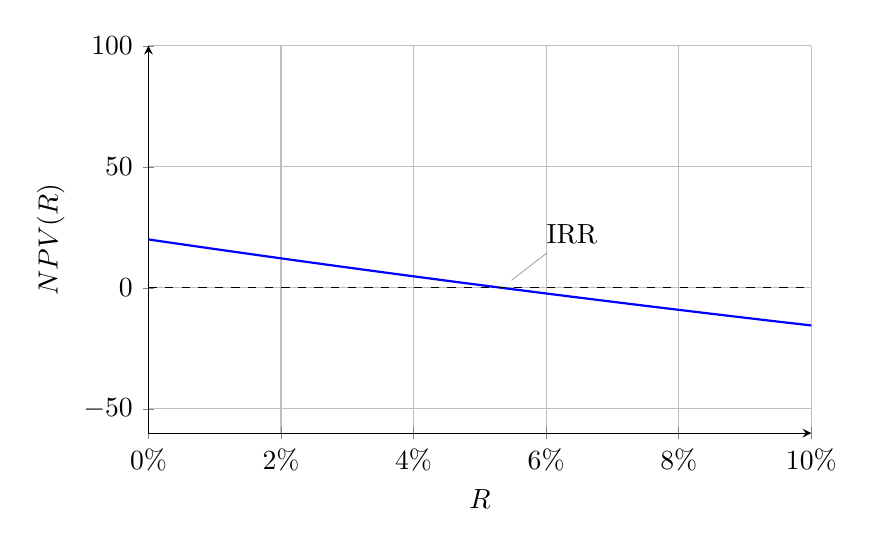
\begin{tikzpicture}
\begin{axis}[
  width=10cm, height=6.5cm,
  xlabel={$R$}, ylabel={$NPV(R)$},
  xmin=0, xmax=0.10, ymin=-60, ymax=100,
  xtick={0,0.02,0.04,0.06,0.08,0.10},
  xticklabel={\pgfmathparse{\tick*100}\pgfmathprintnumber{\pgfmathresult}\%},
  axis lines=left,
  grid=major]
\addplot[domain=0:0.10, samples=60, thick, blue]
  {200/(1+x) + 100/(1+x)^2 - 280};
\addplot[domain=0:0.10, samples=2, black, dashed] {0};
\node[pin=45:{IRR}] at (axis cs:0.0533,0) {};
\end{axis}
\end{tikzpicture}
\caption{NPV法とIRR法のイメージ。$NPV(R)$ は単調減少関数であり，横軸との交点が
IRR である。IRR と WACC の比較で投資判断を行う。}
\label{fig:npv-irr}
\end{figure}

\begin{example}[例題2-2]
以下の2種類の投資がある。
\begin{description}
\item[投資A.] 現時点で280億円の投資をすると，1年後に200億円，2年後に100億円の
キャッシュフローが確実に得られる。
\item[投資B.] 現時点で280億円の投資をすると，1年後に150億円，2年後に150億円の
キャッシュフローが確実に得られる。
\end{description}
(どちらも合計300億円が得られる設定である。)
\begin{enumerate}
\item[(1)] どちらに投資すべきか，IRR法を用いて判断しなさい。
\item[(2)] 割引率 $R = 4.5\%$ として，NPV法を用いて2種類の投資の妥当性について
述べなさい。
\end{enumerate}

\medskip
\noindent\textbf{解答。}
(1) 投資Aについて，IRR は
\[
\frac{200}{1+R} + \frac{100}{(1+R)^2} - 280 = 0
\]
の解であり，$R_A = 5.3342\%$。同様に投資Bでは
$\frac{150}{1+R} + \frac{150}{(1+R)^2} - 280 = 0$ の解として $R_B = 4.7255\%$ を
得る。IRR が高い投資Aを実行すべきである。

(2) 割引率 $R=4.5\%$ で計算すると，
\begin{align*}
NPV_A &= \frac{200}{1.045} + \frac{100}{1.045^2} - 280 = 2.960555\text{ 億円},\\
NPV_B &= \frac{150}{1.045} + \frac{150}{1.045^2} - 280 = 0.900163\text{ 億円}.
\end{align*}
どちらも $NPV>0$ なので，どちらの投資も合理的である。また，正味現在価値は
投資Aの方が高い。
\end{example}

\vspace{18pt}

\subsection{NPV法・IRR法で十分か?}

実際には，
\begin{itemize}
\item 将来キャッシュフローは不確実である場合が多い。
\item さらに，投資判断を行う時点は延期できることが多い。
\end{itemize}

将来キャッシュフローが不確実な場合の例を見てみよう。以下では一時的に，時間的な
価値の違い(時間による割引の効果)は無視して考える。

\begin{example}[将来キャッシュフローが不確実な場合]
「1年後に，50\%の確率で12億円，50\%の確率で8億円受け取れる」という投資のために
必要な金額が，現在は9億円であるとする。この投資の正味現在価値はいくらか。

正味現在価値の算出に期待値を使うならば，
\[
NPV = 0.5\times 12 + 0.5\times 8 - 9 = 1 > 0
\]
となる。しかし，この結果が $NPV>0$ だからといって，投資すべきと言えるだろうか。
この投資では，確率50\%で1億円の損失が発生する。この損失が投資家の経営に大きな
影響を与えうるとすれば，もう少し慎重に考えるべきではないだろうか。
\end{example}

この損失を重視する投資家は，何らかの(期待値とは別の)形で損失の効果を考慮した
投資評価を行う。\textbf{この評価の方法を提供するのが，金融工学}である。本講義の
後半で説明する。

\subsection*{参考：古いプロジェクト評価法}

参考までに，古いプロジェクト評価法を挙げる(講義では特に注意を払わなくて
よいとされた)。
\begin{itemize}
\item \textbf{回収期間法} (payback period method)：既に述べた。
\item \textbf{割引回収期間法} (discounted payback period method)：回収期間を，
回収額でなく，回収額の現在価値で求めたもの。
\item \textbf{収益性指標法} (profitability index method)：
(投資による将来CFの現在価値)/(初期投資額) $> 1$ ならば投資する。
\end{itemize}

% ---------------- 演習問題 ----------------
\section{演習問題}

\begin{exercise}[問題2-1]
複利利回り(年率)を5\%とする。
\begin{enumerate}
\item[(1)] いま100円投資したときの，3年後の価値(終価)。
\item[(2)] 3年後の100円の現在価値(現価)。
\end{enumerate}
これらを，(A) 1年複利，(B) 半年複利，(C) 3ヶ月複利，(D) 連続複利，のそれぞれの
場合について求めなさい。
\end{exercise}

\begin{answerbox}
\textbf{考え方。}例題2-1と同じ計算を，期間 $n=3$ 年に伸ばしたものである。
離散時間の一般形\eqref{eq:discrete-general}より，転化回数 $m$ のとき
\[
\text{終価} = 100\Bigl(1+\frac{0.05}{m}\Bigr)^{3m},
\qquad
\text{現価} = 100\Bigl(1+\frac{0.05}{m}\Bigr)^{-3m}
\]
であり，連続複利では式\eqref{eq:continuous-general}より終価 $100e^{0.05\times 3}$，
現価 $100e^{-0.05\times 3}$ となる。

\medskip
\textbf{計算。}
\begin{itemize}
\item[(A)] 1年複利($m=1$)：終価 $100\times 1.05^3 = 115.763$ 円，
現価 $100\times 1.05^{-3} = 86.384$ 円。
\item[(B)] 半年複利($m=2$)：終価 $100\times 1.025^6 = 115.969$ 円，
現価 $100\times 1.025^{-6} = 86.230$ 円。
\item[(C)] 3ヶ月複利($m=4$)：終価 $100\times 1.0125^{12} = 116.075$ 円，
現価 $100\times 1.0125^{-12} = 86.151$ 円。
\item[(D)] 連続複利：終価 $100e^{0.15} = 116.183$ 円，
現価 $100e^{-0.15} = 86.077$ 円。
\end{itemize}

\medskip
\textbf{ポイント。}同じ年率5\%でも，転化回数が多いほど再投資の効果が働いて終価は
大きくなり，その分だけ現価は小さくなる。連続複利が両者の極限(終価は上限，現価は
下限)を与える。
\end{answerbox}

\begin{exercise}[問題2-2]
例題2-2の設定のもとで，さらにもう一つの投資案件も考慮する。
\begin{description}
\item[投資C.] 現時点で280億円の投資をすると，1年後に100億円，2年後に200億円の
キャッシュフローが確実に得られる。
\end{description}
\begin{enumerate}
\item[(1)] どれに投資すべきか，IRR法を用いて判断しなさい。
\item[(2)] 割引率 $R = 4.5\%$ として，NPV法を用いて投資Cの妥当性について
述べなさい。
\end{enumerate}
\end{exercise}

\begin{answerbox}
\textbf{考え方。}投資Cは合計金額こそ投資A・Bと同じ300億円だが，大きい方の
キャッシュフロー(200億円)を受け取るのが2年後と遅い。時間価値を考えると，
同じ合計額でも受取が遅いほど価値は低いはずである。このことを IRR と NPV で
定量的に確認する。

\medskip
\textbf{(1) IRR法。}投資Cの IRR は
\[
\frac{100}{1+R} + \frac{200}{(1+R)^2} - 280 = 0
\]
の解である。これを解くと($x=1+R$ とおけば $280x^2 - 100x - 200 = 0$ という
2次方程式になる)$R_C = 4.2385\%$ を得る。3案件を並べると：
\vspace{0.9em}
\begin{center}
\begin{tabular}{lccc}
\toprule
時点 & 投資A & 投資B & 投資C\\
\midrule
0(投資額) & 280 & 280 & 280\\
1年後 & 200 & 150 & 100\\
2年後 & 100 & 150 & 200\\
\midrule
IRR & 5.3342\% & 4.7255\% & 4.2385\%\\
\bottomrule
\end{tabular}
\end{center}
\vspace{0.9em}
この結果より，IRR が最も高い\textbf{投資Aを実行すべき}である。

\medskip
\textbf{(2) NPV法。}割引率 $R=4.5\%$ として
\[
NPV_C = \frac{100}{1.045} + \frac{200}{1.045^2} - 280 = -1.16023\text{ 億円} < 0.
\]
\vspace{0.9em}
\begin{center}
\begin{tabular}{lccc}
\toprule
 & 投資A & 投資B & 投資C\\
\midrule
NPV(億円) & 2.960555 & 0.900163 & $-1.16023$\\
\bottomrule
\end{tabular}
\end{center}
\vspace{0.9em}
投資Cは正味現在価値がマイナスになるので，\textbf{非合理的な投資}と判断できる。

\medskip
\textbf{ポイント。}IRR と NPV の判定は整合的である。すなわち，
\[
\text{割引率} < IRR \;\to\; NPV > 0,
\qquad
\text{割引率} > IRR \;\to\; NPV < 0
\]
であり，NPV は $R$ の単調関数なので逆向きも成立する。実際，投資Cでは
IRR($4.2385\%$)$<$ 割引率($4.5\%$)なので $NPV<0$ となっている。また，
受取合計額が同じ300億円でも，早い時点に多く受け取る投資Aほど IRR・NPV ともに
高い。これはキャッシュフローの時間価値そのものである。
\end{answerbox}

% 第3章 金利の期間構造(資料3)
\chapter{金利の期間構造}

利回りは投資期間(残存期間)によって異なる値をとる.この「期間と利回りの関係」を
\textbf{金利の期間構造} (term structure of interest rates) という.本章では,
将来のキャッシュフローが確定している場合を考え,安全確実な債券($\approx$ 国債)を
対象として,最終利回り,イールドカーブ,ゼロレート,フォワード・イールドという
一連の概念を学ぶ.

\section*{導入:国債利回りのデータ}

講義では,日本相互証券が公表する10年国債利回りデータ(BB国債価格(引値))を
もとに,各年度末時点の利回りカーブが示された.残存期間(年)を横軸,複利利回り
(\%)を縦軸にとると,例えば次のような特徴が観察される.

\begin{itemize}
\item 2026年3月末:残存期間とともに利回りが上昇する右上がりのカーブで,
10年で2\%を超える水準.
\item 2025年3月末:同じく右上がりで,10年で1.5\%前後.
\item 2024年3月末:右上がりで,10年で0.7\%程度.
\item 2023年2月末:短期はマイナス圏($-0.1\%$前後)から始まり,10年で0.5\%程度.
\item 2022年2月末:短期が$-0.05\%$程度,10年で0.2\%弱.
\item 2021年3月末:短中期が広くマイナス圏で,10年でようやく0.1\%程度.
\item 2020年3月末:7年超までほぼフラット(マイナス圏)という特異な形状.
\end{itemize}

このように,利回りは残存期間ごとに異なり,カーブ全体の水準も形状も時期によって
大きく変化する.また,2000年代(2000〜2007年の各年度末)の国債の金利期間構造
(ゼロレートカーブ)を重ねて描くと,どの年も右上がり(順イールド)であることが
確認できる.本章はこの「期間構造」を記述する道具立てを与える.

\section{最終利回りと債券価格}

\subsection{証券の現在価値とディスカウントファクター}

複数回の確定的な将来キャッシュフローの場合,前章で学んだとおり,
\[
\text{証券の現在価値} = \text{(将来キャッシュフローの現在価値の総和)}
= \sum_i \bigl\{(\text{時刻 } t_i \text{ の将来CF}) \times
(\text{時刻 } t_i \text{ における1円の現在価値})\bigr\}
\]
である.「ある証券を持つこと」と「その証券から生じる個々の将来キャッシュフローを
個々の契約とみなし,すべての契約をまとめたものを持つこと」の経済価値は同じであり,
後者で考える方がわかりやすい.

時刻 $t$ のキャッシュフローを $CF(t)$,時刻 $t$ における1円の現在価値を
$DF(t)$ と書く.キャッシュフローのある時点を $t_i$, $i=1,2,\dots,N$ とすると,
現在価値 $PV$ は
\begin{equation}
PV = \sum_{i=1}^{N} CF(t_i)\, DF(t_i).
\label{eq:pv-df}
\end{equation}

\begin{definition}[ディスカウントファクター]
将来時点 $t$ における1円の現在価値 $DF(t)$ を,\textbf{ディスカウント
ファクター}(ディスカウントファンクション,割引関数)と呼ぶ.
\end{definition}

\subsection{最終利回りの定義}

額面 $F$ 円,満期2年,クーポンレート $C$,年1回払の満期一括償還の利付債を
考える.価格を $P$ として,
\begin{equation}
P = \frac{FC}{1+Y} + \frac{FC}{(1+Y)^2} + \frac{F}{(1+Y)^2}
\end{equation}
という式を満たす $Y$ を\textbf{最終利回り} (Yield To Maturity, YTM) と呼ぶ.

同じ債券でも年2回払であれば,複利の設定(転化回数 $m$)に応じて式が変わり,
\begin{equation}
P = \frac{FC/2}{1+Y/2} + \frac{FC/2}{(1+Y/2)^2} + \frac{FC/2}{(1+Y/2)^3}
+ \frac{FC/2}{(1+Y/2)^4} + \frac{F}{(1+Y/2)^4}
\end{equation}
となる.

\begin{definition}[最終利回り(一般形)]
額面 $F$ 円,満期 $N$ 年,クーポンレート $C$,年 $m$ 回払の満期一括償還の
利付債の価格を $P$ とするとき,
\begin{equation}
P = \frac{F}{(1+Y/m)^{mN}} + \sum_{j=1}^{mN}\frac{FC/m}{(1+Y/m)^{j}}
\label{eq:ytm-def}
\end{equation}
を満たす $Y$ を\textbf{最終利回り} (Yield To Maturity) と呼ぶ.
\end{definition}

前章までの考え方によると,式\eqref{eq:ytm-def}は「満期まで一定の利回り $Y$ を
用いて将来キャッシュフローを割り引いた現価(現在価値)が $P$」と読める.

\begin{keypoint}[債券価格と最終利回りの関係]
債券価格 $P$ と最終利回り $Y$ は,\textbf{逆方向に動く}.一方が上がれば他方は
下がり,一方が下がれば他方は上がる.すなわち関数 $P(Y)$ は単調減少である.
最終利回り $Y$ は,価格 $P$ を利回りで言い換えたものである.
\end{keypoint}

講義資料では次の2つの例が図示された.
\begin{itemize}
\item 5年満期割引国債(額面100円):最終利回りが0\%のとき価格100円,利回りが
上がるにつれて価格は単調に下落し,5\%で約78円となる.
\item 10年満期,クーポンレート3\%,額面100円,満期一括償還の利付債:利回り0\%の
とき価格130円,\textbf{最終利回り $=$ クーポンレートのとき価格はちょうど100円}
(パー)となり,8\%では約66円まで下がる.
\end{itemize}
最終利回りとクーポンレートが等しいとき価格が額面に一致することは,
式\eqref{eq:ytm-def}に $Y=C$ を代入すると等比数列の和が畳み込めて $P=F$ となる
ことから確認できる(まず1期間のケースで確かめるとよい).

\begin{example}[例題3-1:債券の現在価値]
額面100円,満期2年,クーポンレート6\%,半年払い($m=2$)の債券の現在価値を
求めなさい.
\begin{enumerate}
\item[(1)] 複利利回りを5\%(半年複利)とする場合.
\item[(2)] 連続複利利回りを5\%とする場合.
\end{enumerate}

\medskip
\noindent\textbf{解答.}
キャッシュフローは,0.5年,1年,1.5年後に各3円($=6\%\times 100\times 0.5$),
2年後に103円である.

(1) 半年複利のディスカウントファクターは $DF(t) = (1+0.05/2)^{-2t}$ であるから,
\[
PV = \sum_{i=1}^{4} CF(0.5i)\,DF(0.5i)
= \frac{3}{1+\frac{0.05}{2}} + \frac{3}{(1+\frac{0.05}{2})^2}
+ \frac{3}{(1+\frac{0.05}{2})^3} + \frac{103}{(1+\frac{0.05}{2})^4}
\approx 101.88.
\]

(2) 連続複利のディスカウントファクターは $DF(t) = e^{-0.05t}$ であるから,
\[
PV = 3e^{-0.05\times 0.5} + 3e^{-0.05\times 1} + 3e^{-0.05\times 1.5}
+ 103e^{-0.05\times 2} \approx 101.76.
\]

計算の内訳は次表のとおりである.
\begin{center}
\small
\begin{tabular}{cccc@{\qquad}cccc}
\toprule
\multicolumn{4}{c}{半年複利(利回り5.0\%)} & \multicolumn{4}{c}{連続複利(利回り5.0\%)}\\
\cmidrule(r){1-4}\cmidrule(l){5-8}
年 & CF & DF & 価値 & 年 & CF & DF & 価値\\
\midrule
0.5 & 3 & 0.97561 & 2.92683 & 0.5 & 3 & 0.97531 & 2.92593\\
1.0 & 3 & 0.95181 & 2.85544 & 1.0 & 3 & 0.95123 & 2.85369\\
1.5 & 3 & 0.92860 & 2.78580 & 1.5 & 3 & 0.92774 & 2.78323\\
2.0 & 103 & 0.90595 & 93.31292 & 2.0 & 103 & 0.90484 & 93.19825\\
\midrule
\multicolumn{3}{r}{現在価値} & 101.88099 & \multicolumn{3}{r}{現在価値} & 101.7611\\
\bottomrule
\end{tabular}
\end{center}
\end{example}

\subsection{価格から最終利回りを求める}

定義式\eqref{eq:ytm-def}に沿って,価格 $P$ から最終利回り $Y$ を算出することを
考える.一般に,これは $mN$ 次方程式を解くことになるため,$mN \geq 2$ では
$Y$ を求めるには数値計算が必要である.

注意点として,(高次方程式なので)不適切な解も存在しえるため,結果をチェックする
必要がある.とはいえ,$Y$ を求める関数はエクセルにも実装されていて,一般的に
使われている.

\section{イールドカーブ}

\begin{definition}[イールドカーブ(利回り曲線)]
個々の債券について,残存期間を $x$ 座標,利回りを $y$ 座標として平面上に
描いた線(カーブ)のこと.利回りの期間構造(利回り曲線)ともいう.
\end{definition}

利回りにはいろいろな種類のものがあるが,債券投資の実務では「最終利回り」が
よく使われる.

カーブの概形については次の用語がある.
\begin{itemize}
\item \textbf{順イールド} (normal yield):右上がりのカーブ.
\item \textbf{逆イールド} (inverted yield):右下がりのカーブ.
\end{itemize}
実際には順イールドになることが多い.このほか,中間の期間が盛り上がった
humped shape と呼ばれる形状もある.

先に見た2026年3月末の10年国債利回りカーブは典型的な順イールドである.一方,
2020年3月末のカーブは,7年超までほぼフラットでマイナス圏という形状であり,
「順イールド?」と問いたくなるような特異な例であった.また,2000〜2007年の
各年度末のゼロレートカーブ(後述)はいずれも右上がり,すなわち順イールドである.

\section{ゼロ(クーポン)・レート}

\subsection{最終利回りは使い難い?}

属性のうち,クーポンレートだけが異なる2つの債券の価格を考える.
\[
P_1 = \frac{F}{(1+Y_1)^N} + \sum_{i=1}^{N}\frac{FC_1}{(1+Y_1)^i},
\qquad
P_2 = \frac{F}{(1+Y_2)^N} + \sum_{i=1}^{N}\frac{FC_2}{(1+Y_2)^i}.
\]
通常,クーポンレート $C$ が違えば,価格 $P$ も最終利回り $Y$ も異なる.
すると,次のような疑問が生じる.

\begin{itemize}
\item 同一発行体の同時点のキャッシュフローを割り引くとき,クーポンレートが違う
債券では\emph{異なる}最終利回りで割り引くことになるのか?
\item 同一債券では,どの時点のキャッシュフローも\emph{同じ}利回りで割り引くことに
なるのか?
\end{itemize}

これらの疑問への一つの答え方は,「上記の式を割引の式と深く考えるな」,すなわち
これらは単にキャッシュフローと価格の関係(価格を利回りで言い換えたもの)と
みなせ,というものである.

\subsection{期間を代表する利回り:ゼロレート}

残存期間ごとに一意に決まる「期間を代表する利回り」を使って現在価値への割引を
行えば,話はスッキリする.では,期間を代表する利回りとして何を使えばよいか.
最終利回り $Y$ は,債券の条件(クーポンレートなど)が違うと値が変わる,という
問題が生じる.これを回避するのが次のゼロレートである.

\begin{definition}[ゼロレート]
\textbf{ゼロレート} (zero rate),\textbf{ゼロクーポンレート} (zero-coupon rate)
とは,割引債の最終利回りのことである.(“ゼロクーポン債=割引債”である.)
\end{definition}

残存期間を決めると,ゼロレートは一つに決まる(もし異なる値をとるならば,同満期の
割引債で価格が違うことになってしまう).したがって,
\begin{itemize}
\item ゼロレートは残存期間の代表的な金利として使える.
\item 異なる債券のキャッシュフローでも,同じ時点のキャッシュフローは,残存期間で
決まるゼロレートで割り引けばよい.
\end{itemize}
この考え方の転換は,講義では「ゼロレート革命」と呼ばれた.

\subsection{ゼロレートによる債券価格評価}

設定:年1回利払い,$N$ 年満期,額面 $F$ 円.$P$ を現在の価格,$C_i$ を $i$ 年目の
クーポン,$r_i$ を $i$ 年のゼロレートとする.ディスカウントファクター(割引関数)
$DF(i)$ は「$i$ 年後の1円の現価」であり,
\begin{equation}
DF(i) = \frac{1}{(1+r_i)^i} = (1+r_i)^{-i}
\label{eq:df-zero}
\end{equation}
と書ける.このとき債券価格は
\begin{equation}
P = \frac{C_1}{1+r_1} + \frac{C_2}{(1+r_2)^2} + \cdots + \frac{C_N}{(1+r_N)^N}
+ \frac{F}{(1+r_N)^N}
= \sum_{i=1}^{N} C_i\,DF(i) + F\,DF(N).
\label{eq:price-zero}
\end{equation}
なお,$DF(i)$ は $i$ 年満期の(額面1円の)割引債価格でもある.

\subsection{ゼロレートとYTMによる価格式の比較}

ゼロレートを用いた価格式と,最終利回りを用いた価格式を並べると,
\[
P = \sum_{i=1}^{N}\frac{C_i}{(1+r_i)^i} + \frac{F}{(1+r_N)^N}
\qquad\text{vs.}\qquad
P = \sum_{i=1}^{N}\frac{C_i}{(1+Y)^i} + \frac{F}{(1+Y)^N}.
\]
両者の違いに注意する.形式的には,右の式(最終利回りの定義式)は,利回りの
期間構造をフラットと仮定して CF を割り引いて現価を求めている形である.しかし,
これを「割引」とは考えないほうが,おそらくスッキリする(最終利回りは価格の
言い換えに過ぎない).

\subsection{連続複利における割引関数}

$DF(T) = D(T)$ を連続複利で表す.ゼロレートを $r_i$ として,$1/m$ 年複利で
$m\to\infty$ のケースを考えると,
\begin{equation}
D(T) = \lim_{m\to\infty}\Bigl(1+\frac{r_i}{m}\Bigr)^{-mT}
= \lim_{m\to\infty}\Biggl[\Bigl(1+\frac{1}{m/r_i}\Bigr)^{m/r_i}\Biggr]^{-r_i T}
= e^{-r_i T}.
\label{eq:df-cont}
\end{equation}
これが連続複利の(すなわち連続時間モデルにおける複利の)割引関数である.

\begin{remark}[イールドカーブの縦軸とスポット・レートという言葉]
イールドカーブ(金利期間構造)の縦軸を,債券の最終利回りでなく,ゼロレートを
使って表示することもよく行われる.特に理論の論文では,ゼロレートの方がよく
用いられる.一方,債券実務では今も最終利回りを使うことが多く,かつ取引は今も
単利である.

なお,実務では,現時点で取引されているゼロレートを\textbf{スポット・レート}
(spot rate) と呼ぶことがある.もともと「スポット」は直物(現時点で取引される
商品)を意味する.しかし,理論でスポットレートというと,少し別の意味(瞬間的な
短期金利という意味,本章付録参照)で使われることも多い.「スポット」は複数の
意味で使われる言葉なので,注意を要する.
\end{remark}

\section{フォワード・イールド}

本節の言葉の使い方はやや理論家寄りである(言葉の使い方はその人次第であり,
証券アナリストのテキストとは異なることもある).引き続き,安全確実な債券
($\approx$ 国債)を考える.

\subsection{イールド}

時刻を $t$ で表す.現在を $t=0$ として,$0 \le t \le T \le \tau$ とする.

\begin{definition}[イールド]
$Y(t,T)$:\textbf{イールド}.期間 $[t,T]$ の平均利回り.
\begin{itemize}
\item $t=0$ ならば,$Y(0,T)$ は確定値.
\item $t>0$ ならば,$Y(t,T)$ は確率変数(現時点 $t=0$ で値は確定しない).
\end{itemize}
\end{definition}

以下では,割引債による運用を考えて利回りについて記述する.割引債は株式と違い
キャッシュフローが確定的で考えやすいからである(株式の場合は,利回りと言っても
よいが,収益率と呼ぶ).定義より,$Y(0,T)$ が時刻 $t=0$ における期間 $T$ の
ゼロレートに相当する.

\subsection{運用と運用成果}

ある資産での運用を考える.時刻 $t$ における1単位あたりの価格を $p(t)$ とする.
期間 $[t,T]$ の運用成果を考える.投資額を $A$ 円とすると,
\begin{itemize}
\item $A / p(t)$:時刻 $t$ における購入量.
\item $A \times p(T)/p(t)$:時刻 $T$ における運用成果.
\item $p(T)/p(t)$:期間 $[t,T]$ の $(1+\text{利回り})$.
\end{itemize}

\begin{example}
期間 $[t,T]$ における,満期 $T$ の割引債(価格 $v(t,T)$)による(時刻 $t$ の)
1円の(時刻 $T$ における)運用成果は,
\[
1 \times \frac{v(T,T)}{v(t,T)} = \frac{1}{v(t,T)}.
\qquad(\because\ v(T,T)=1.)
\]
\end{example}

\subsection{フォワード・イールド}

\begin{definition}[フォワード・イールド]
時点 $t$ でみた,将来の期間 $[T,\tau]$($t \le T \le \tau$)の利回りを
\textbf{フォワード・イールド}といい,$f(t,T,\tau)$ と書く.
\end{definition}

定義から $Y(T,\tau) = f(T,T,\tau)$ である.$Y(T,\tau)$ は普通は時刻 $T$ に
ならないと確定しない.そんな利回りを $T$ 以前の時刻 $t$ で予想しても,その
予想値は確定値であろうはずがない.\emph{しかし},時刻 $t$ で取引されている
満期の異なる割引債を使うことで,この利回りを時刻 $t$ で確定させることもできる.
これが次のインプライド・フォワード・イールドである.

\subsection{現時点でフォワード・イールドは確定できる}

とりあえず $t=0$ として考える.いま取引されている(=スポットの)ゼロレートを
使うことで,将来のある期間の利回りを確定することができる.

\begin{example}[フォワード・イールドの確定]
ゼロレートが1年で5\%,2年で6\%とする.このとき,
\begin{itemize}
\item 満期1年の割引債(額面105万円)を空売りし,代金100万円を受け取る.
ここで $v(0,1) = DF(1) = 1/(1+0.05)$ なので,額面105万円の1年割引債の現在の
価格はちょうど $105 \times v(0,1) = 100$ 万円である.
\item その全額100万円で,満期2年の割引債(額面112.36万円)を買う.
$v(0,2) = DF(2) = 1/(1+0.06)^2$ なので,100万円で買える額面は
$100/v(0,2) = 100\times 1.06^2 = 112.36$ 万円である.
\end{itemize}
この合成ポジションのキャッシュフローは次のとおりである.
\begin{center}
\begin{tabular}{c|cc|cc|cc}
\toprule
時点(年) & \multicolumn{2}{c|}{1年割引債の売り} & \multicolumn{2}{c|}{2年割引債の買い}
& \multicolumn{2}{c}{合計}\\
 & 収入 & 支出 & 収入 & 支出 & 収入 & 支出\\
\midrule
0 & 100 & & & 100 & &\\
1 & & 105 & & & & 105\\
2 & & & 112.36 & & 112.36 &\\
\bottomrule
\end{tabular}
\end{center}
合計をみると,現時点のキャッシュフローはゼロで,「1年後に105万円を支払い,
2年後に112.36万円を受け取る」という取引になっている.すなわち,\textbf{この
取引で,1年後から2年後までの期間の利回りが現時点で確定}している.その利回りは
$112.36/105 - 1 \approx 7.01\%$ である.
\end{example}

\subsection{インプライド・フォワード・イールド}

\begin{definition}[インプライド・フォワード・イールド]
前項の方法で(市場で取引されている割引債・ゼロレートを使って)確定させた
フォワード・イールドを,\textbf{インプライド (implied)・フォワード・イールド}と
いう.
\end{definition}

この値は,1年物と2年物のゼロレートによって決まる値,つまり時刻 $t$ における
市場の状態によって決まる値である.

\begin{remark}
これを単にフォワード・イールドと呼ぶ人も,フォワード・レートと呼ぶ人も,
インプライド・フォワード・レートと呼ぶ人もいる.そのため,言葉の意味を確認
しながら使わないと危ない.
\end{remark}

インプライド・フォワード・イールドの話は一般化できる.記法として
\begin{itemize}
\item $Y(i,j,j+k)$:時点 $i$ における $j$ 期間から $(j+k)$ 期間までの利回り,
\item $Y(i,i+j)$:時点 $i$ における $j$ 期間の利回り(ゼロレート),
\end{itemize}
を用いる.基本となる考え方は次である.

\begin{keypoint}[裁定の考え方]
どういう期間区分で運用しても,($N$ 年後の)終価は同じ.少なくとも均衡状態では
そのようになっているはずである.(瞬間的にはズレるし,別の理由でズレが維持される
こともあるが.)
\end{keypoint}

例えば3年間の運用は,「3年ゼロレートでの一括運用」「1年目はゼロレート
$Y(0,1)$,残り2年はフォワード $Y(0,1,3)$」「1年ずつ $Y(0,0,1)$, $Y(0,1,2)$,
$Y(0,2,3)$ とつなぐ運用」のいずれでも同じ終価になる.

\subsection{インプライド・フォワード・イールドの公式(1年複利)}

\begin{example}[例1:2年間の投資]
1年目をゼロレート $Y(0,1)$ で,2年目をフォワード・イールド $Y(0,1,2)$ で運用した
成果と,2年ゼロレート $Y(0,2)$ で運用した成果は等しいので,
\[
\bigl(1+Y(0,1)\bigr)\bigl(1+Y(0,1,2)\bigr) = \bigl(1+Y(0,2)\bigr)^2
\qquad\therefore\quad
Y(0,1,2) = \frac{(1+Y(0,2))^2}{1+Y(0,1)} - 1.
\]
\end{example}

\begin{example}[例2:$j$ 年後から $j+k$ 年後の間の投資]
\[
\bigl(1+Y(0,j)\bigr)^{j}\bigl(1+Y(0,j,j+k)\bigr)^{k}
= \bigl(1+Y(0,j+k)\bigr)^{j+k}
\]
\[
\therefore\quad
Y(0,j,j+k) = \Biggl(\frac{(1+Y(0,j+k))^{j+k}}{(1+Y(0,j))^{j}}\Biggr)^{1/k} - 1.
\]
\end{example}

このように,\textbf{インプライド・フォワード・イールドはゼロレートで書ける}.
すなわち,「ゼロレートの期間構造」から「インプライド・フォワード・イールド
(の期間構造)」を求めることができる.

\begin{example}[例3:1年間の投資]
\[
Y(0,0,1) = Y(0,1).
\]
すなわち,最初の1期間のフォワード・イールドはゼロレートそのものである.
\end{example}

\begin{example}[例4:$N$ 年間の投資]
\[
\bigl(1+Y(0,0,1)\bigr)\bigl(1+Y(0,1,2)\bigr)\cdots\bigl(1+Y(0,N-1,N)\bigr)
= \bigl(1+Y(0,N)\bigr)^{N}
\]
\[
\therefore\quad
Y(0,N) = \sqrt[N]{\bigl(1+Y(0,0,1)\bigr)\bigl(1+Y(0,1,2)\bigr)\cdots
\bigl(1+Y(0,N-1,N)\bigr)} - 1.
\]
\end{example}

逆に,\textbf{ゼロレートはインプライド・フォワード・イールドで書ける}.
例4の形から,ゼロレートはインプライド・フォワード・イールドの期間平均
(幾何平均)的な値であることがわかる.この関係から,次が成り立つ.

\begin{keypoint}[カーブの形状の関係]
インプライド・フォワード・イールド・カーブが右上がり(右下がり,水平)ならば,
ゼロレート・カーブも右上がり(右下がり,水平)である.この関係は常に成立する.
しかし,\textbf{逆は常に成り立つとは限らない}(ゼロレート・カーブが右上がりでも,
フォワード・カーブが右上がりとは限らない).
\end{keypoint}

\subsection{インプライド・フォワード・イールドの公式(連続複利)}

\begin{example}[{例1:2年間(一般には $[j,j+k]$)の投資}]
連続複利では,運用成果の等式は指数の和になる:
\[
e^{j\,Y(0,j)}\,e^{k\,Y(0,j,j+k)} = e^{(j+k)\,Y(0,j+k)}
\qquad\therefore\quad
Y(0,j,j+k) = \frac{(j+k)\,Y(0,j+k) - j\,Y(0,j)}{k}.
\]
\end{example}

\begin{example}[例2:$N$ 年間の投資]
\[
e^{Y(0,0,1)}\,e^{Y(0,1,2)}\cdots e^{Y(0,N-1,N)} = e^{N\,Y(0,N)}
\qquad\therefore\quad
Y(0,N) = \frac{Y(0,0,1) + Y(0,1,2) + \cdots + Y(0,N-1,N)}{N}.
\]
\end{example}

連続複利の場合,\textbf{ゼロレートはインプライド・フォワード・イールドの期間
加重平均値}(単純平均)になる.

\subsection{割引債価格との関係}

\paragraph{(1) $t=0$ の場合.}
現在($t=0$)について考える.時刻 $t=0$ の満期 $T$,額面1円の割引債価格を
$v(0,T)$ と書く.ゼロレート $Y(0,T)$ との関係は,
\begin{align}
\text{1年複利:}\quad & v(0,T) = \bigl(1+Y(0,T)\bigr)^{-T},\notag\\
\text{半年複利:}\quad & v(0,T) = \bigl(1+Y(0,T)/2\bigr)^{-2T},\notag\\
\text{$1/m$年複利:}\quad & v(0,T) = \bigl(1+Y(0,T)/m\bigr)^{-mT},\notag\\
\text{連続複利:}\quad & v(0,T) = e^{-T\,Y(0,T)}.
\label{eq:v0T}
\end{align}
$v(0,T)$ は時刻 $t=0$(現在)における割引関数で,$t=0$ で既知である.

\paragraph{(2) インプライド・フォワード・イールドと割引債価格($t=0$).}
$Y(0,T,\tau)$ をインプライド・フォワード・イールド($t=0$ では既知)とすると,
\begin{align}
\text{1年複利:}\quad & Y(0,T,\tau)
= \Bigl(\frac{v(0,T)}{v(0,\tau)}\Bigr)^{1/(\tau-T)} - 1,\notag\\
\text{半年複利:}\quad & Y(0,T,\tau)
= 2\Bigl[\Bigl(\frac{v(0,T)}{v(0,\tau)}\Bigr)^{1/2(\tau-T)} - 1\Bigr],\notag\\
\text{$1/m$年複利:}\quad & Y(0,T,\tau)
= m\Bigl[\Bigl(\frac{v(0,T)}{v(0,\tau)}\Bigr)^{1/m(\tau-T)} - 1\Bigr],\notag\\
\text{連続複利:}\quad & Y(0,T,\tau)
= \frac{\log\bigl(v(0,T)/v(0,\tau)\bigr)}{\tau-T}.
\label{eq:fwd-v}
\end{align}
これらの導出は演習問題3-4である.導出の鍵は,$[0,T]$ 間の運用成果は
$\mathrm{price}(T)/\mathrm{price}(0)$ であり,満期 $T$ までの割引債 $v(0,T)$ の
運用成果は $1/v(0,T)$($\because v(T,T)=1$)であることである.

\begin{remark}
理論では,割引債価格を額面1円で考えて,割引関数とみなすのが普通である.実務では,
割引債でも債券なので,額面100円で価格を考える.
\end{remark}

\paragraph{(3)(4) $t>0$ の場合.}
ここまでは現在($t=0$)だけ考えたので $Y(0,\cdot)$ や $Y(0,\cdot,\cdot)$ と
したが,$t>0$ にしても考え方は同じである.ただし,変数はすべて確率変数になる.
時刻 $t$ の満期 $T$,額面1円の割引債価格を $v(t,T)$ と書くと,
\begin{align}
\text{1年複利:}\quad & v(t,T) = \bigl(1+Y(t,T)\bigr)^{-(T-t)},\notag\\
\text{半年複利:}\quad & v(t,T) = \bigl(1+Y(t,T)/2\bigr)^{-2(T-t)},\notag\\
\text{$1/m$年複利:}\quad & v(t,T) = \bigl(1+Y(t,T)/m\bigr)^{-m(T-t)},\notag\\
\text{連続複利:}\quad & v(t,T) = e^{-(T-t)\,Y(t,T)},
\end{align}
であり($v(t,T)$, $t>0$ は時刻 $t$ の割引関数で,$t=0$(現在)では確率変数),
インプライド・フォワード・イールド $Y(t,T,\tau)$(確率変数)についても
\begin{align}
\text{1年複利:}\quad & Y(t,T,\tau)
= \Bigl(\frac{v(t,T)}{v(t,\tau)}\Bigr)^{1/(\tau-T)} - 1,\notag\\
\text{半年複利:}\quad & Y(t,T,\tau)
= 2\Bigl[\Bigl(\frac{v(t,T)}{v(t,\tau)}\Bigr)^{1/2(\tau-T)} - 1\Bigr],\notag\\
\text{$1/m$年複利:}\quad & Y(t,T,\tau)
= m\Bigl[\Bigl(\frac{v(t,T)}{v(t,\tau)}\Bigr)^{1/m(\tau-T)} - 1\Bigr],\notag\\
\text{連続複利:}\quad & Y(t,T,\tau)
= \frac{\log\bigl(v(t,T)/v(t,\tau)\bigr)}{\tau-T}
\end{align}
が成り立つ.

\section*{付録:スポット・レートとフォワード・レート}

デリバティブの実務では,これらが確率変動するモデルを使い,金利期間構造の変動を
議論する.

\subsection*{(瞬間的な)フォワードレート}

フォワード・イールド $f(t,T,\tau)$ の定義で,$\tau = T + dT$ として $dT\to 0$ の
極限を考えたものが,\textbf{(瞬間的な)フォワードレート}である:
\begin{equation}
f(t,T) = \lim_{\Delta T\to 0} Y(t,T,T+\Delta T).
\end{equation}
フォワード・レートは,時刻 $t$ でみた,$[T, T+dT]$ 間の一瞬の利回りである.

$t=0$ の場合を連続複利の式\eqref{eq:fwd-v}で考えると,
\begin{equation}
f(0,t) = \lim_{\Delta t\to 0} Y(0,t,t+\Delta t)
= \lim_{\Delta t\to 0}
\frac{(t+\Delta t)\,Y(0,t+\Delta t) - t\,Y(0,t)}{\Delta t}
= \frac{\dd\,[\,t\,Y(0,t)\,]}{\dd t}.
\end{equation}
これより,
\begin{equation}
\int_0^t f(0,s)\,\dd s = t\,Y(0,t)
\qquad\therefore\quad
Y(0,t) = \frac{1}{t}\int_0^t f(0,s)\,\dd s.
\end{equation}

同様に,$t>0$,つまり将来においても,満期変数($T$)についての微分として
\begin{equation}
f(t,T) = \frac{\dd\,[\,(T-t)\,Y(t,T)\,]}{\dd T}
\end{equation}
となるので,
\begin{equation}
\int_t^T f(t,s)\,\dd s = (T-t)\,Y(t,T)
\qquad\therefore\quad
Y(t,T) = \frac{1}{T-t}\int_t^T f(t,s)\,\dd s.
\end{equation}

このように,現在および将来のゼロレートはフォワードレートで記述できる.
したがって,\textbf{フォワードレート $f(t,T)$ の変動過程を上手にモデル化すれば,
金利期間構造の全体の変動を上手に表現できる}.これが現在の確率金利モデルの
基本的な考え方である.

\subsection*{(瞬間的な)スポットレート}

(瞬間的な)フォワードレート $f(t,T)$ の $T \to t$ の極限値を,
\textbf{(瞬間的な)スポットレート}という:
\begin{equation}
r(t) = \lim_{T\to t} f(t,T).
\end{equation}
スポット・レートは,時刻 $t$ でみた,$[t, t+dt]$ の一瞬の利回りである.
スポットレート $r(t)$ の変動過程を上手にモデル化しても,金利期間構造の変動を
上手に表現できる.デリバティブの価格付けでは,$r(t)$ や $f(t,T)$ を確率過程と
して扱ったモデルがよく使われる.

% ---------------- 演習問題 ----------------
\section{演習問題}

\begin{exercise}[問題3-1:債券価格と最終利回り]
額面100円,満期3年,クーポンレート2\%,半年払い($m=2$)の債券の,将来
キャッシュフローと現在価値を求めなさい.ただし,半年複利の最終利回りは3\%と
する.
\end{exercise}

\begin{answerbox}
\textbf{考え方.}まずキャッシュフローを書き出す.クーポンは
$C_i = K\times F\times(t_i - t_{i-1}) = 2\%\times 100\times 0.5 = 1$ 円
(半年ごと)であり,満期3年には額面100円が加わって101円となる.次に,各時点の
1円の現価(ディスカウントファクター)$DF(t) = (1+0.03/2)^{-2t}$ を掛けて
合計する.

\medskip
\textbf{計算.}
\begin{center}
\begin{tabular}{cccc}
\toprule
年 & キャッシュフロー & 1円の現価 & キャッシュフローの現価\\
\midrule
0.5 & 1 & 0.9852 & 0.9852\\
1.0 & 1 & 0.9707 & 0.9707\\
1.5 & 1 & 0.9563 & 0.9563\\
2.0 & 1 & 0.9422 & 0.9422\\
2.5 & 1 & 0.9283 & 0.9283\\
3.0 & 101 & 0.9145 & 92.3688\\
\midrule
\multicolumn{3}{r}{債券価格} & 97.1514\\
\bottomrule
\end{tabular}
\end{center}
よって現在価値(債券価格)は約 \textbf{97.15円}である.

\medskip
\textbf{ポイント.}クーポンレート(2\%)が最終利回り(3\%)より低いので,価格は
額面100円を下回る(アンダーパー).「最終利回り $=$ クーポンレート $\iff$
価格 $=$ 額面」という関係とあわせて確認しておくとよい.
\end{answerbox}

\begin{exercise}[問題3-2:インプライド・フォワード・イールドとゼロレート(離散時間モデル)]
次の表の空欄のインプライド・フォワード・イールドとゼロレートの値を求めなさい.
ただし,1年を一期間とする離散時間モデルで考える.
\begin{center}
\small
\begin{tabular}{c|cc|cc|cc}
\toprule
 & \multicolumn{2}{c|}{ケースA} & \multicolumn{2}{c|}{ケースB}
 & \multicolumn{2}{c}{ケースC}\\
年 & フォワード & ゼロ & フォワード & ゼロ & フォワード & ゼロ\\
\midrule
1 & 7.0\% & 7.000\% & 5.0\% & --- & --- & 9.0\%\\
2 & 7.0\% & --- & 6.0\% & --- & --- & 8.5\%\\
3 & 7.0\% & --- & 7.0\% & --- & --- & 8.0\%\\
4 & 7.0\% & --- & 8.0\% & --- & --- & 7.5\%\\
5 & 7.0\% & --- & 9.0\% & --- & --- & 7.0\%\\
\bottomrule
\end{tabular}
\end{center}
※ 表の「フォワードレート」は「インプライド・フォワード・イールド」に読み替える.
表中のフォワード・イールドは,それぞれ運用期間1年間のインプライド・フォワード・
イールドの意味である.例えば,ケースBの5年の9.0\%は $f(0,4,5)$,つまり現時点で
みた4年から5年の1年間の投資期間の利回りであり,4年の8.0\%は $f(0,3,4)$ である.
\end{exercise}

\begin{answerbox}
\textbf{考え方.}$n$ 年のゼロレート $r_n$ と1年刻みのフォワード・イールド
$f_j = f(0,j-1,j)$ の間には,「どの期間区分で運用しても $n$ 年後の終価は同じ」
という関係
\[
(1+r_n)^n = (1+f_1)(1+f_2)\cdots(1+f_n)
\]
が成り立つ.フォワードからゼロを求めるにはこの式をそのまま使い,ゼロから
フォワードを求めるには
\[
1+f_n = \frac{(1+r_n)^n}{(1+r_{n-1})^{n-1}}
\]
を使う.

\medskip
\textbf{計算結果.}
\begin{center}
\small
\begin{tabular}{c|cc|cc|cc}
\toprule
 & \multicolumn{2}{c|}{ケースA} & \multicolumn{2}{c|}{ケースB}
 & \multicolumn{2}{c}{ケースC}\\
年 & フォワード & ゼロ & フォワード & ゼロ & フォワード & ゼロ\\
\midrule
1 & 7.0\% & 7.000\% & 5.0\% & 5.000\% & 9.000\% & 9.0\%\\
2 & 7.0\% & 7.000\% & 6.0\% & 5.499\% & 8.002\% & 8.5\%\\
3 & 7.0\% & 7.000\% & 7.0\% & 5.997\% & 7.007\% & 8.0\%\\
4 & 7.0\% & 7.000\% & 8.0\% & 6.494\% & 6.014\% & 7.5\%\\
5 & 7.0\% & 7.000\% & 9.0\% & 6.991\% & 5.023\% & 7.0\%\\
\bottomrule
\end{tabular}
\end{center}
例えばケースBの2年ゼロレートは
$r_2 = \sqrt{1.05\times 1.06} - 1 = 5.499\%$,ケースCの2年フォワードは
$f_2 = 1.085^2/1.09 - 1 = 8.002\%$ である.

\medskip
\textbf{ポイント.}
\begin{itemize}
\item ケースA:フォワードが常に7\%なら,ゼロレートも常に7\%(フラット).
\item ケースB:フォワードが右上がりのとき,ゼロレートも右上がりになるが,
ゼロレートはフォワードの「平均」なので,伸びはフォワードより緩やか.
\item ケースC:ゼロレートが右下がりのとき,フォワードはそれより急な右下がりに
なる.
\end{itemize}
ゼロレートはインプライド・フォワード・イールドの平均値的なものである.しかし,
離散時間モデルでは(幾何平均のため)微妙にズレる.連続時間モデルでは,まさに
期間平均値になる.
\end{answerbox}

\begin{exercise}[問題3-3:ゼロレートと債券価格]
額面100円,残存期間3年,クーポンレート6\%(年1回払い)の満期一括償還の利付債を
考える.
\begin{enumerate}
\item ゼロレートが1年で5\%,2年で6\%,3年で7\%のとき,利付債の価格と最終利回りを
求めなさい.
\item ゼロレートが1年で7\%,2年で6\%,3年で5\%のとき,利付債の価格と最終利回りを
求めなさい.
\end{enumerate}
ただし,1年を一期間とする離散時間モデルで考えること.
\end{exercise}

\begin{answerbox}
\textbf{考え方.}価格は,各時点のキャッシュフロー(1・2年目:6円,3年目:106円)を
それぞれの残存期間のゼロレートで割り引いて合計する(式\eqref{eq:price-zero}).
最終利回りは,得られた価格 $P$ に対して
$P = \sum_{i=1}^{3} CF_i/(1+Y)^i$ を満たす $Y$ を数値的に求める.

\medskip
\textbf{1.(順イールドのケース)}
\begin{center}
\small
\begin{tabular}{ccccc}
\toprule
年 & Cash Flow & Zero Rate & Discount Function & Present Value\\
\midrule
1 & 6.00 & 5.000\% & 0.952381 & 5.71429\\
2 & 6.00 & 6.000\% & 0.889996 & 5.33998\\
3 & 106.00 & 7.000\% & 0.816298 & 86.52757\\
\midrule
\multicolumn{4}{r}{PRICE} & 97.58184\\
\multicolumn{4}{r}{YTM} & 6.920\%\\
\bottomrule
\end{tabular}
\end{center}

\textbf{2.(逆イールドのケース)}
\begin{center}
\small
\begin{tabular}{ccccc}
\toprule
年 & Cash Flow & Zero Rate & Discount Function & Present Value\\
\midrule
1 & 6.00 & 7.000\% & 0.934579 & 5.60748\\
2 & 6.00 & 6.000\% & 0.889996 & 5.33998\\
3 & 106.00 & 5.000\% & 0.863838 & 91.56679\\
\midrule
\multicolumn{4}{r}{PRICE} & 102.51424\\
\multicolumn{4}{r}{YTM} & 5.075\%\\
\bottomrule
\end{tabular}
\end{center}

\medskip
\textbf{ポイント.}どちらのケースもゼロレートは 5\%,6\%,7\% の同じ3つの値から
なるが,並び順が違うだけで価格も最終利回りも大きく異なる.1.では YTM
$=6.920\%$ と3年ゼロレート(7\%)に近く,2.では YTM $=5.075\%$ と3年ゼロレート
(5\%)に近い.これは,この債券のキャッシュフローの大部分(106円)が3年目に
あるためである.すなわち,\textbf{YTM は,キャッシュフローが大きな時点の
ゼロレートを強く反映}する.
\end{answerbox}

\begin{exercise}[問題3-4:割引債価格との関係]
\begin{enumerate}
\item[(1)] 割引債価格とゼロレートの関係式\eqref{eq:v0T}を導出しなさい.
\item[(2)] インプライド・フォワード・イールドと割引債価格の関係式
\eqref{eq:fwd-v}を導出しなさい.
\end{enumerate}
\end{exercise}

\begin{answerbox}
\textbf{(1) の解答.}
割引債価格 $v(0,T)$ は,$t=0$(現在)における割引関数 $DF(T)$ とみなせる
(額面1円の割引債の価格は「$T$ 年後の1円の現価」そのものである).よって,
離散時間モデルの複利表示の式は,ディスカウントファクターの式
\eqref{eq:df-zero}(を $1/m$ 年複利に一般化したもの)
\[
v(0,T) = DF(T) = \Bigl(1+\frac{Y(0,T)}{m}\Bigr)^{-mT}
\]
から得られる.連続時間モデルの連続複利表示の式は,連続複利の割引関数の式
\eqref{eq:df-cont}から $v(0,T) = e^{-T\,Y(0,T)}$ として得られる.

\medskip
\textbf{(2) の解答.}
代表として半年複利の式(2番目の式)を示す.0年から $T$ 年まで割引債で運用し,
$T$ 年から $\tau$ 年までインプライド・フォワード・イールドで運用した成果は
\[
\frac{1}{v(0,T)}\times\Bigl(1+\frac{Y(0,T,\tau)}{2}\Bigr)^{2(\tau-T)}.
\]
一方,0年から $\tau$ 年まで割引債で運用したときの成果は $1/v(0,\tau)$ である.
均衡ではこれらは等しいので,
\[
\frac{1}{v(0,T)}\Bigl(1+\frac{Y(0,T,\tau)}{2}\Bigr)^{2(\tau-T)}
= \frac{1}{v(0,\tau)}
\]
が成り立ち,これを $Y(0,T,\tau)$ について解けば
\[
Y(0,T,\tau) = 2\Bigl[\Bigl(\frac{v(0,T)}{v(0,\tau)}\Bigr)^{1/2(\tau-T)} - 1\Bigr]
\]
を得る.1年複利・$1/m$ 年複利の式(1番目と3番目の式)も同様に得られる.

連続複利の式(4番目の式)も同様である.0年から $T$ 年まで割引債で運用し,
$T$ 年から $\tau$ 年までインプライド・フォワード・イールドで運用した成果は
\[
\frac{1}{v(0,T)}\times e^{(\tau-T)\,Y(0,T,\tau)}
\]
であり,これが $1/v(0,\tau)$ に等しいことから
\[
\frac{1}{v(0,T)}\,e^{(\tau-T)\,Y(0,T,\tau)} = \frac{1}{v(0,\tau)}
\qquad\therefore\quad
Y(0,T,\tau) = \frac{\log\bigl(v(0,T)/v(0,\tau)\bigr)}{\tau-T}.
\]

\medskip
\textbf{ポイント.}導出の本質は「運用成果の一致(裁定が働けば,どの経路で運用
しても同じ期間の確定運用成果は等しい)」である.割引債の運用成果が $1/v(0,T)$ と
書けること($v(T,T)=1$)さえ押さえれば,あとは機械的に式変形できる.
\end{answerbox}

% 第4章 リターン,リスクと効用(資料4)
\chapter{リターン,リスクと効用}

前章までは将来のキャッシュフローが確定的な世界を扱った.本章からは,将来が
\emph{不確実}な資産(株式など)を扱うための道具立てを導入する.鍵になるのは,
収益率を確率変数とみなす見方,その分布を要約する\textbf{リターン}と
\textbf{リスク},投資家の選好を記述する\textbf{効用関数}と\textbf{期待効用原理},
そしてリスク負担の対価である\textbf{リスク・プレミアム}である.

\section*{導入:株価チャート}

日経平均株価などの株価チャートには,次のような要素が描かれている.

\begin{itemize}
\item \textbf{ローソク足}:一定期間(日足,週足,月足)の\textbf{始値}(はじめね),
\textbf{終値}(おわりね),\textbf{高値}(たかね),\textbf{安値}(やすね)を
1本の「ローソク」で表したもの.
\item \textbf{移動平均線}:過去5日,25日,75日,150日などの終値の平均を
つないだ線.
\item \textbf{出来高(売買高)}:片道数量(売りと買いで一つの取引とした数量)で,
単位は株.ただし,市場が活況か否かという実態は,株数よりも\textbf{売買代金}の方が
よく表現している.大雑把な活況の目安は1日あたり2兆円である.
\end{itemize}

\section{投資収益率}

\subsection{算術収益率}

時刻 $t$ における価格を $P_t$,時刻 $t+1$ における価格を $P_{t+1}$,時刻 $t+1$ に
おける配当を $D_{t+1}$($\geq 0$)とする.

\begin{definition}[算術収益率]
(一期間あたりの)\textbf{算術収益率} $R_{t+1}$ を
\begin{equation}
R_{t+1} = \frac{P_{t+1} - P_t + D_{t+1}}{P_t}
= \frac{P_{t+1} + D_{t+1}}{P_t} - 1
\label{eq:arith-return}
\end{equation}
と定義する.
\end{definition}

分子のうち,$P_{t+1} - P_t$ の部分は,正なら\textbf{キャピタル・ゲイン},負なら
キャピタル・ロスと呼ばれる.$D_{t+1}$ の部分は\textbf{インカム}(インカム・
ゲイン)と呼ばれる.

\subsection{対数収益率}

\begin{definition}[対数収益率]
(一期間あたりの)\textbf{対数収益率} $R^{\log}_{t+1}$ を
\begin{equation}
R^{\log}_{t+1} = \log\frac{P_{t+1}+D_{t+1}}{P_t}
= \log(P_{t+1}+D_{t+1}) - \log P_t
= \log\Bigl(1 + \frac{P_{t+1}-P_t+D_{t+1}}{P_t}\Bigr)
\label{eq:log-return}
\end{equation}
と定義する.
\end{definition}

テーラー展開による近似式 $\log(1+x) \approx x$($|x| \ll 1$ のとき)を用いると,
\begin{equation}
R^{\log}_{t+1} = \log\Bigl(1 + \frac{P_{t+1}-P_t+D_{t+1}}{P_t}\Bigr)
\approx \frac{P_{t+1}-P_t+D_{t+1}}{P_t} = R_{t+1}
\end{equation}
となり,収益率の数値が小さければ対数収益率と算術収益率はほとんど変わらない.

\subsection{対数収益率と算術収益率の違い}

通常,収益率の数値は小さいので両者の値はほとんど変わらないが,\textbf{時系列上の
対称性}に違いがある.

\begin{example}
時系列で価格が 100円 $\to$ 105円 $\to$ 100円と変動したときを考える.
\begin{itemize}
\item 算術収益率では,$5/100 = 5.00\%$,$-5/105 = -4.76\%$ で,平均は $0.12\%$.
\item 対数収益率では,$\log(105/100) = 4.88\%$,$\log(100/105) = -4.88\%$ で,
平均は $0.00\%$.
\end{itemize}
価格が元に戻ったのに算術収益率の平均は正になる一方,対数収益率は(時間に関して)
対称性があり,平均はちょうど0になる.
\end{example}

時系列で収益率を扱う際は,対称性がある方が好ましいと考えられている.ただし,
どちらの方が優れているか,という話ではない.実際,
\begin{itemize}
\item リスク管理では,\textbf{対数収益率}がよく使われる.
\item ポートフォリオの最適化では,\textbf{算術収益率}がよく使われる.
\end{itemize}

\subsection{収益率の分布}

日経平均の日次収益率(1984年1月5日〜2008年11月14日)のヒストグラムを,同じ
平均・分散をもつ正規分布と重ねて描くと,次のことが観察される.

\begin{itemize}
\item 実際の分布は,正規分布に比べて中心が高く尖っている.
\item 裾を拡大して見ると,正規分布ではほとんど起こりえないような大きな下落
(例えば1987年10月20日,ブラックマンデー翌日の約$-15\%$)が実際には起きている.
すなわち,実際の分布は正規分布より\textbf{裾が厚い}(ファット・テイル).
\item 週次収益率(1984年1月4日〜2008年11月10日)でも同様で,2008年10月6日の週
(リーマンショック時)には$-25\%$前後の下落が生じている.
\end{itemize}

このように収益率は日々変動する.そこで,\textbf{収益率は何らかの分布を持つ
確率変数である}と考える.分布を記述する統計量については,
\begin{itemize}
\item 期待値($=$平均値)は水準感の目安になるが,それだけでは情報不足である.
\item 収益率の日々の「変動の大きさ」を示す指標が必要であり,
「分散」または「標準偏差」といった2次の統計量を使用する.
\item 3次以上の統計量(歪度・尖度など)が使われることもある.
\end{itemize}

\section{リターン,リスク}

\subsection{定義}

収益率を確率変数 $R$ とし,観測データを $R_i$, $i=1,2,\dots,N$ とする.

\begin{definition}[リターンとリスク]
\textbf{リターン(期待収益率)}は収益率の期待値 $\E[R]$ であり,観測データからは
\begin{equation}
\E[R] = \frac{1}{N}\sum_{i=1}^{N} R_i
\end{equation}
と推定される.\textbf{リスク}は収益率の標準偏差である.
\end{definition}

なお,「リターン」を(期待値でなく)収益率そのものの意味で使い,期待値の方を
「期待リターン」と言うこともある.人によって定義が違うので注意が必要である.

\subsection{ボラティリティ}

\begin{definition}[ボラティリティ]
収益率の標準偏差を\textbf{ボラティリティ} (volatility) と呼ぶ.省略するときは
「ボラ」または「vol」.
\end{definition}

講義資料では,2012年9月〜2013年6月の日経平均株価について,日々の終値,対数
収益率,および「日々の収益率は独立同一分布に従う」と仮定して過去20日間の収益率
から求めたボラティリティ(年率換算)の時系列が示された.この期間,株価は
約8,800円から15,000円超まで大きく上昇し(いわゆるアベノミクス相場),日次収益率は
$\pm 2\%$程度の変動から,2013年前半には$\pm 6\%$を超える激しい変動へと拡大,
年率換算ボラティリティも15\%程度から45\%超へと大きく変動した.

このように過去データから直接求めたボラティリティを,\textbf{ヒストリカル・
ボラティリティ} (historical volatility) と呼ぶ.
\begin{itemize}
\item データをとる期間は20日間に限らない.
\item データにウェイトをつけること(直近を重視する等)もある.
\end{itemize}
(ヒストリカル・)ボラティリティは重要なリスク尺度の一つであり,
「ボラティリティが高い」$=$「リスクは高い」と考える.

また,利回り(金利)も変動する.1M・6M・12MのLIBORの長期時系列(1996〜2020年頃)
を見ると,金利水準が高い状態と低い状態を行き来しており,こうした動きは
レジーム・スイッチング・モデル (Regime Switching Model) による分析の対象にも
なっている.

実務では,リスク(ボラティリティ)の情報は重視される一方,リターンの情報は
それほど強調されない.リターン(平均)の推定は本質的に難しく,不安定である
ことがその一因である.

\begin{remark}[金融リスク管理におけるリスク]
ボラティリティ,標準偏差,分散などは,\textbf{金融リスク管理では}リスクの大きさを
示す適切な尺度とは考えられていない.なぜならば,これらは平均(あるいは想定水準)
からの乖離の大きさを示すが,リスク管理では想定よりも\emph{儲かる}ことをリスクとは
考えず,\emph{損失のみ}がリスクだからである.そこで,リスク管理向けの(下落量を
示す)尺度が考案されている.例として,VaR (Value at Risk),ES (Expected
Shortfall) などがある.
\end{remark}

\section{効用,効用関数,期待効用原理}

\subsection{どちらを選びますか?}

次の2つの選択問題を考えてみよう.

\begin{enumerate}
\item 安全資産:1年後に\emph{確実に}1万円得られる.危険資産:1年後に20\%の
確率で5万円得られ,80\%の確率で何ももらえない.どちらも5,000円で購入できる.
では,どちらを選ぶ?(期待収益(5,000円)は等しくしてある.)
\item 安全資産:1年後に\emph{確実に}10億円得られる.危険資産:1年後に20\%の
確率で50億円得られ,80\%の確率で何ももらえない.どちらも5億円で購入できる.
では,どちらを選ぶ?(期待収益(5億円)は等しくしてある.)
\end{enumerate}

多くの人は,特に金額が大きい2.では,安全資産を選ぶのではないだろうか.期待収益が
同じでも,不確実な方を避けるこのような選好を,次のように定式化する.

\subsection{リスク回避的投資家}

\begin{keypoint}[リスク回避的投資家]
通常,合理的な投資家は\textbf{リスク回避的}と考える.リスク回避的な投資家は,
\begin{itemize}
\item リターンが同じならば,リスクの小さい方を選ぶ.
\item リスクが同じならば,リターンが大きい方を選ぶ.
\end{itemize}
(ここでは,リターン $=$ 期待収益率.)
\end{keypoint}

なお,別のタイプの投資家として,\textbf{リスク中立的}な投資家,
\textbf{リスク愛好的}な投資家もいる.では,これらの選好を数学的にはどのように
記述するのか.それが以下の効用関数である.

\subsection{効用と効用関数}

$w$ を\textbf{富}または財(金銭・土地・株式・サービス等,価値あるモノの量),
$u$ を\textbf{効用}(富を持つ,またはサービスを受けることで得られる満足度)と
する.

\begin{definition}[効用関数]
次の2つの仮定を必ず満たす関数 $u(w)$ を\textbf{効用関数}という.
\begin{itemize}
\item 仮定1.効用 $u$ は,富 $w$ の関数 $u(w)$ である.
\item 仮定2.富が多いほど,満足度は高い.すなわち
\begin{equation}
u'(w) = \frac{\dd u(w)}{\dd w} > 0.
\end{equation}
\end{itemize}
$u'(w)$ を\textbf{限界効用} (marginal utility) と呼ぶ.
\end{definition}

\subsection{期待効用原理}

\begin{definition}[期待効用原理]
投資家は,自分の効用の数学的期待値 $\E[u(W)]$ を最大化するように行動する
(機会選択を行う).ここで富 $W$ は確率変数である.
\end{definition}

\begin{example}[確率的な富か,期待値相当の確定的な富か]
期待効用原理の下で,投資家は (i) 確率変数の富 $W$,(ii) 期待値相当分の確定的な富
$\E[W]$,のどちらを選択するか?

\textbf{解答.}期待効用原理に従うと,(i) の $\E[u(W)]$ と (ii) の $u(\E[W])$ の
うち,大きい方を選ぶことになる.どちらを選ぶことになるかは $u(w)$ の性質,特に
2階導関数 $\dd^2 u(w)/\dd w^2$ 次第である.
\end{example}

\subsection{Jensenの不等式}

\begin{theorem}[Jensenの不等式]
$f(x)$ が凸関数,$X$ が確率変数のとき,
\begin{equation}
f(\E[X]) \leq \E[f(X)]
\end{equation}
が成り立つ.
\end{theorem}

ここで\textbf{凸関数}とは,$0 < \lambda < 1$ に対して
\begin{equation}
f(\lambda x + (1-\lambda)y) \leq \lambda f(x) + (1-\lambda) f(y)
\end{equation}
が成り立つ関数のことである(内分点の関数値 $\leq$ 関数値の内分点).
\textbf{凹関数}は,$-f(x)$ が凸関数になる関数のことであり,$f$ が凹関数ならば,
Jensenの不等式の不等号の向きは逆になる.

Jensenの不等式は演算の交換に関する不等式の一つであり,ここでは期待値演算と
関数演算の交換に対応している.$X$ が $x_1, x_2$ を各確率0.5でとる場合を図で
考えると,$f(\E[X])$ は曲線上の中点での値,$\E[f(X)]$ は2点の関数値の中点で
あり,凸関数では後者の方が大きいことが図からも見てとれる.

\subsection{効用関数の凹凸とリスク選好}

先の「確率的な富 $W$ か,確定的な富 $\E[W]$ か」の選択は,効用関数の凹凸で
次のように整理できる.

\begin{keypoint}[効用関数の凹凸とリスク選好]
\begin{itemize}
\item $u(w)$ が\textbf{凹関数}($\dd^2u/\dd w^2 < 0$)$\Rightarrow$
$u(\E[W]) \geq \E[u(W)]$ $\Rightarrow$ 確定的な富 $\E[W]$ を選択
(\textbf{リスク回避的}).
\item $u(w)$ が\textbf{凸関数}($\dd^2u/\dd w^2 > 0$)$\Rightarrow$
$u(\E[W]) \leq \E[u(W)]$ $\Rightarrow$ 確率的な富 $W$ を選択
(\textbf{リスク愛好的}).
\item $u(w)$ が\textbf{一次関数}($\dd^2u/\dd w^2 = 0$,凹関数かつ凸関数)
$\Rightarrow$ $u(\E[W]) = \E[u(W)]$ $\Rightarrow$ どちらも選択対象
(\textbf{リスク中立的}).
\end{itemize}
\end{keypoint}

したがって,リスク回避的な投資家の効用関数は
\begin{equation}
u'(w) = \frac{\dd u(w)}{\dd w} > 0 \quad(\text{狭義単調増加関数}),
\qquad
u''(w) = \frac{\dd^2 u(w)}{\dd w^2} < 0 \quad(\text{凹関数})
\end{equation}
という性質をもつ.

\begin{figure}[htbp]
\centering
\begin{tikzpicture}[scale=1.0]
\begin{axis}[
  width=9cm, height=6.5cm,
  xlabel={$w$}, ylabel={$u(w)$},
  xmin=0, xmax=10, ymin=0, ymax=3.6,
  xtick={1,5,9},
  xticklabels={$w_1$,$\E[W]$,$w_2$},
  ytick=\empty,
  axis lines=left]
\addplot[domain=0.3:10, samples=80, thick, blue] {sqrt(x)};
% chord
\addplot[domain=1:9, samples=2, red, dashed] {1 + (3-1)/(9-1)*(x-1)};
% points
\draw[dotted] (axis cs:1,0) -- (axis cs:1,1);
\draw[dotted] (axis cs:9,0) -- (axis cs:9,3);
\draw[dotted] (axis cs:5,0) -- (axis cs:5,2.236);
\draw[dotted] (axis cs:0,2.236) -- (axis cs:5,2.236);
\draw[dotted] (axis cs:0,2) -- (axis cs:5,2);
\node[left] at (axis cs:0,2.236) {\small $u(\E[W])$};
\node[left] at (axis cs:0,2.0) {\small $\E[u(W)]$};
\end{axis}
\end{tikzpicture}
\caption{リスク回避的(凹)な効用関数.富 $W$ が $w_1,w_2$ を各確率0.5でとる
とき,$\E[u(W)]$(赤い弦の中点の高さ)よりも $u(\E[W])$(曲線上の値)の方が
大きい.}
\label{fig:concave-utility}
\end{figure}

\subsection{限界効用逓減の法則}

経済学には\textbf{限界効用逓減(ていげん)の法則}がある.すなわち,富が増える
につれて,1単位の富の追加がもたらす満足度の上昇量は減少していく.これは限界効用
$u'(w)$ が富の単調減少関数であること,すなわち
\begin{equation}
u''(w) = \frac{\dd}{\dd w}\Bigl(\frac{\dd u(w)}{\dd w}\Bigr) < 0
\end{equation}
を意味している.これが成立するのは,リスク回避的な効用関数を用いる場合である.

\subsection{よく使われるリスク回避的な効用関数}

\begin{itemize}
\item \textbf{べき(型)効用関数}:
$u(w) = w^{\gamma}$,\quad $0<\gamma<1$ または $\gamma < 0,\ \gamma\neq 0$.
\item \textbf{指数(型)効用関数}:
$u(w) = -e^{-aw}$,\quad $a>0$.
\item \textbf{対数(型)効用関数}:
$u(w) = \log w$.
\item (※)\textbf{二次効用関数}:
$u(w) = aw - \tfrac{1}{2}bw^2$,\quad $a>0,\ b\geq 0,\ w \leq a/b$.
単調増加する部分のみ使用する.
\end{itemize}

\begin{example}[指数効用による議論の例]
効用関数を $u(w) = -e^{-aw}$($a>0$)とし,富 $W$ の分布は
\[
W = \begin{cases} u & \text{確率 } 0.5,\\ v & \text{確率 } 0.5,\end{cases}
\qquad u < v
\]
とする.投資家は,このまま富 $W$ を保有してもよいし,富の期待値分 $\E[W]$ を
保有することにしてもよい,とする.どちらを選択するか.

$\E[W] = (u+v)/2$ を保有するときの効用は
\[
u(\E[W]) = -e^{-a(u+v)/2},
\]
このまま $W$ を保有したときの期待効用は
\[
\E[u(W)] = -\bigl(e^{-au} + e^{-av}\bigr)/2
\]
である.これらの大小関係をみるために,相加相乗平均の関係式
\[
\frac{a+b}{2} \geq \sqrt{ab},\qquad a>0,\ b>0
\]
を使う.すると,
\[
\E[u(W)] = -\frac{e^{-au}+e^{-av}}{2}
\leq -\sqrt{e^{-au}\times e^{-av}}
= -e^{-a(u+v)/2}
= u(\E[W]).
\]
これより,確実に平均的な富 $\E[W]$ を得られる方を選択する.指数効用では
リスク回避的な投資家の選択と同じになることが確認できた.
\end{example}

\section{リスク・プレミアム}

リスク・プレミアムは,価格にリスクを反映させる際の調整項である.

\subsection{リスク・プレミアムとは}

先の「どちらを選びますか?」の危険資産を,リスク回避的な投資家は購入しない.

\begin{itemize}
\item[問.] では,どうすればリスク回避的な投資家は危険資産でも購入するように
なるのか?
\item[答.] 購入することで抱えるリスクに見合うだけの収益を得られるならば,
危険資産であっても購入する.
\end{itemize}

つまり,危険資産\emph{だから}購入しないのではなく,収益がリスクに見合わないと
考えるから購入しないのである.収益とリスクのバランスが大切である.

\begin{definition}[リスク・プレミアム]
リスクをとること(リスク・テイク)に対する対価(超過収益)を
\textbf{リスク・プレミアム} (risk premium) と呼ぶ.
\end{definition}

では,どれだけの大きさのリスク・プレミアムをとればよいのか.以下では2つの
考え方を示す.

\subsection{確実性等価原理}

定数 $X = 100$,確率変数 $W = 200$(確率50\%)or $0$(確率50\%)とする.
これまでの議論より,リスク回避的投資家では $u(\cdot)$ が凹関数なので
$u(\E[W]) > \E[u(W)]$.ゆえに $X = \E[W]$(安全資産)を選択する.

これを\emph{価格}で考える.安全利子率は $r$(一定)とする.1年後の
キャッシュフロー $X$(確定値)の現在価値は $X/(1+r)$ である.では,1年後の
キャッシュフロー $W$(確率変数)の現在価値はどう評価すべきか.$W$ は確率変数
なので,$X$ とまったく同じ評価をすることはできない.次の2つの考え方がある.

\paragraph{考え方A(割引率の調整項としてのリスク・プレミアム).}
キャッシュフローの期待値 $\E[W]$ を,\textbf{リスク調整済割引率} $R > r$ で
割り引く.すなわち $W$ の現在価値を
\begin{equation}
\text{現在価値} = \frac{\E[W]}{1+R} = \frac{\E[W]}{1 + r + (R-r)}
\end{equation}
とし,差 $R - r$ を\textbf{リスク・プレミアム}と呼ぶ.

これは,学術的な議論よりも実務で時々見られる考え方である.例えば,国が発行する
債券(国債)の利回り $r$ と,一般事業会社が発行する債券(社債)の利回り $R$ の
差 $R-r$ が市場で提示されている.$R-r$(リスク・プレミアム)が高いほどリスクが
高い.例えば,格付が低いほど $R-r$ は高くなる.つまり(同じキャッシュフローに
対して)社債の価格は安くなる.

\paragraph{考え方B(財の調整項としてのリスク・プレミアム).}
効用関数 $u$ を使い,
\begin{equation}
u(w^*) = \E[u(W)]
\label{eq:certainty-equiv}
\end{equation}
を満たす定数 $w^*$ を求め,$W$ の現在価値を $w^*/(1+r)$ とする.つまり,
\begin{enumerate}
\item 効用関数の値が期待効用と同じ値になる富 $w^*$ を求め,
\item その富を\emph{安全利子率} $r$ を使って割り引くことで,現在価値を求める.
\end{enumerate}
この考え方を\textbf{確実性等価原理},$w^*$ を\textbf{確実性等価}と呼ぶ.
このときのリスク・プレミアムは
\begin{equation}
c = \E[W] - w^* = \E[W] - u^{-1}\bigl(\E[u(W)]\bigr)
\end{equation}
であり,富の大きさの低減量(富の大きさへの調整項)である.$c$ はリスク・テイクに
対する対価の大きさを示している(価値を低くすることで,収益率を高めている).

シンプルな確率的な富 $W$($w_1$ または $w_2$ を各確率0.5でとる)で考えると,
凹関数 $u$ のグラフ上で,$\E[u(W)]$ の高さに対応する曲線上の点の横座標が
$w^*$ であり,$w^* < \E[W]$,その差がリスク・プレミアム $c$ である.一般には,
Jensenの不等式より $u(\E[W]) \geq \E[u(W)]$ かつ $u(\cdot)$ は単調増加なので,
$u(\E[W]-c) = \E[u(W)]$ を満たす $c$ は $c \geq 0$ となる.

\begin{example}[例題4-1]
現在の富を100万円とし,価格 $p$ 万円の宝くじの購入を検討する.その宝くじは,
確率50\%で100万円,確率50\%で何ももらえない.安全利子率を $r$(年率),宝くじの
支払いまでの期間を $\Delta t$ 年とする.効用関数は $u(w) = w^{0.5}$($w$:万円)
とする.

宝くじを「購入する」「購入しない」の選択肢がある.
\begin{itemize}
\item 購入しないときの効用は(現在の富を安全に運用すると考えて)
\[
u\bigl(100\times(1+r\Delta t)\bigr) = \bigl(100(1+r\Delta t)\bigr)^{0.5}.
\]
\item 購入するときの期待効用は(宝くじ購入の支出,残金の安全な運用,宝くじの
結果から)
\[
0.5\bigl((100-p)(1+r\Delta t) + 100\bigr)^{0.5}
+ 0.5\bigl((100-p)(1+r\Delta t) + 0\bigr)^{0.5}.
\]
\end{itemize}
以上より,宝くじを購入すべき条件は
\[
0.5\bigl((100-p)(1+r\Delta t)+100\bigr)^{0.5}
+ 0.5\bigl((100-p)(1+r\Delta t)\bigr)^{0.5}
\geq \bigl(100(1+r\Delta t)\bigr)^{0.5}.
\]

簡単のため $\Delta t = 0$(即座に結果がわかる)とすると,この条件は
\[
0.5\sqrt{200-p} + 0.5\sqrt{100-p} \geq 10
\qquad\Longleftrightarrow\qquad
p \leq 43.75 \text{ (万円)}
\]
となる.

次に,$p = 43.75$ 万円であったとする.このとき,購入しないときの富の効用と,
購入時の期待効用は等しい.そのため,購入時の期待効用の値を与える確定的な富
$w^*$(確実性等価)がわかる:$w^* = 100$(購入しないときの富だから)である.
一方,購入時の富の期待値は($\Delta t = 0$ を使用)
\[
\E[W] = \bigl(\text{初期富}(100) - \text{宝くじ価格}(43.75)\bigr) +
\text{宝くじの期待値}(50) = 56.25 + 50 = 106.25.
\]
よって,財の調整項であるリスク・プレミアム $c$ は
\[
c = \E[W] - w^* = 106.25 - 100 = 6.25 \text{ (万円)}.
\]
\end{example}

\begin{example}[例題4-2]
例題4-1と同じ設定で,現在の富だけを50万円に変える.購入しないときの効用は
$(50(1+r\Delta t))^{0.5}$,購入するときの期待効用は
\[
0.5\bigl((50-p)(1+r\Delta t)+100\bigr)^{0.5}
+ 0.5\bigl((50-p)(1+r\Delta t)\bigr)^{0.5}
\]
であり,購入すべき条件は($\Delta t = 0$ として)
\[
0.5\sqrt{150-p} + 0.5\sqrt{50-p} \geq \sqrt{50}
\qquad\Longleftrightarrow\qquad
p \leq 37.5 \text{ (万円)}.
\]
$p = 37.5$ 万円のとき,確実性等価は $w^* = 50$(購入しないときの富),
$\E[W] = (50 - 37.5) + 50 = 62.5$ なので,リスク・プレミアムは
\[
c = \E[W] - w^* = 62.5 - 50 = 12.5 \text{ (万円)}.
\]
\end{example}

例題4-1と4-2を比べると,\textbf{購入判断の分岐となる宝くじ価格 $p$ も
リスク・プレミアム $c$ も,現在の富に依存}することがわかる(富が少ないほど,
同じ宝くじに払える価格は低く,要求するリスク・プレミアムは大きい).では,
\emph{全員にとって}合理的な宝くじの価格 $p$,リスク・プレミアム $c$ はあるの
だろうか?

\subsection{効用関数,分布の変換,価格}

例題4-1での投資 $W$ の価値は $w^*/(1+r\Delta t) = (\E[W]-c)/(1+r\Delta t) = 100$,
例題4-2では同様に $50$ である.価格を知るには $w^*$ が必要である.例題では
$w^*$ を所与としたが,一般に $w^*$ は $u(w)$ を使って数値計算で求めることになり,
これは大変である.

ここで,もしも $u(w) = w$(リスク中立)ならば,
$w^* = u^{-1}(\E[u(W)]) = \E[W]$ となるから,$w^*$ は簡単に計算できることに
注目する.そこで,次のような発想の転換を行う.

\begin{keypoint}[リスク中立化の発想(preview)]
投資家はリスク中立的($u(w)=w$)とみなして評価するが,それでは現実と異なるので,
辻褄のあうように $W$ の\emph{分布}を変更する.つまり,
\[
(\text{実際の } u(w),\ \text{実際の } W \text{ の分布})
\]
を,それと同じ価格を与える
\[
(\text{リスク中立な } u(w)=w,\ \text{リスク中立な } W \text{ の分布})
\]
に変換して計算する.そのためには,実際のデータからリスク中立な $W$ の分布を
求める必要がある.
\end{keypoint}

これはかなり advanced な話であるが,後の章で学ぶデリバティブの価格付け
(リスク中立化法)の基本発想がここに現れている.

\subsection{Sharpe Ratio(シャープレシオ)}

ここから先は実務的な話である.「リスクに見合うリスク・プレミアムがついているか」
が金融商品の評価の尺度になる.考え方A(割引率の調整項としてのリスク・プレミアム)
で考える.

\begin{definition}[シャープレシオ]
ある資産の期待収益率を $\mu$,ボラティリティを $\sigma$,安全利子率を $r$ と
する.このとき
\begin{equation}
SR = \frac{\mu - r}{\sigma}
\end{equation}
を \textbf{Sharpe Ratio}(シャープ・レシオ,SR)という.
\end{definition}

これは「超過収益率 $\div$ ボラティリティ(orリスク)」であり,その意味は
\textbf{リスク一単位当たりに要求される超過収益率}である.実務では,投資商品の
パフォーマンスを示す尺度として使われる.

\subsection{ファンドのパフォーマンス評価}

\begin{definition}[ファンド]
\textbf{ファンド}とは,投資のために集めた資金,またはその資金による投資運用商品
のこと.
\begin{itemize}
\item \textbf{公募ファンド}:不特定多数からオープンに募集するファンド.投資信託等.
\item \textbf{私募ファンド}:限られた人から集めるファンド.ヘッジファンド等.
\end{itemize}
\end{definition}

SRによるファンドのパフォーマンス評価は次のように行う.
\begin{itemize}
\item 過去の価格データを使用する.
\item 一定期間の収益率,収益率の標準偏差(リスク)を計算し,SRを算出する.
\item SRが高いほどパフォーマンスが良い,と考える(ただし $SR>0$ の場合).
\end{itemize}
なお,SRが良くなくても敢えて投資することもある(分散投資の効果.後述の章で
扱う).

\begin{example}[例題4-3]
資産Aの収益率は,確率50\%で25\%,確率50\%で$-15\%$である.資産Bの収益率は,
確率50\%で30\%,確率50\%で$-20\%$である.安全利子率を2\%として,それぞれの
資産のシャープレシオを求め,どちらの方が投資効率が良いか議論しなさい.

\medskip
\noindent\textbf{解答.}
資産Aは,リターン $0.5\times 25 + 0.5\times(-15) = 5\%$,リスク(収益率の標準
偏差)は平均5\%からの乖離が $\pm 20\%$ なので20\%である.よって
\[
SR_A = \frac{5-2}{20} = 0.15.
\]
資産Bは,リターン $5\%$,リスク25\%なので,
\[
SR_B = \frac{5-2}{25} = 0.12.
\]
SRは資産Aの方が高いので,SRの観点からは資産Aの方が投資効率が良い
(パフォーマンスが良い)と考えられる.
\end{example}

\subsection{インデックス,トラッキング・エラー,IR}

ファンドの収益率だけで評価してよいのだろうか.頑張って成果を出しているファンド
でも,市場全体が落ち込んでいく局面ではどうにもならない.一方で,たいした成果を
出していないように見えるファンドでも,市場全体が上がっているときは Sharpe Ratio
は高くなる.そこで,市場全体の動きを補正して考えることが行われる.

\begin{itemize}
\item \textbf{インデックス}:市場平均価格.市場価格の動向を示す指数.
例:日経225,TOPIX,NYダウ(米),FT100(フッツィー100,英)など.
\item \textbf{パッシブ運用(インデックス運用)}:インデックスの動きに沿った運用.
対義語は\textbf{アクティブ運用}.ちなみに,アクティブファンドは手数料が高めである.
\item \textbf{アクティブ・リターン} $\mu'$:ファンドとインデックスの収益率の差.
収益率そのものでなく,アクティブ・リターンで評価する.
\item $\E[\mu']$:アクティブ・リターンの期待値.
\item $\sigma'$:アクティブ・リターンの標準偏差.これを
\textbf{トラッキング・エラー}と呼ぶ.
\end{itemize}

\begin{definition}[インフォメーション・レシオ]
\begin{equation}
IR = \frac{\E[\mu']}{\sigma'}
\end{equation}
を\textbf{インフォメーション・レシオ} (Information Ratio, IR) という.
\end{definition}

現在は,$\sigma'$(トラッキング・エラー)や IR の方が評価指標としてよく
使われている.

% ---------------- 演習問題 ----------------
\section{演習問題}

\begin{exercise}[問題4-1]
現在の富を100万円とし,価格 $p$ 万円の宝くじの購入を検討する.その宝くじは,
確率5\%で500万円,確率95\%で10万円もらえるものとする.効用関数は
$u(w) = w^{0.5}$($w$:万円)とする.
\begin{enumerate}
\item[(1)] 購入が合理的と考えられるときの宝くじの価格 $p$ の条件を求めなさい.
\item[(2)] 価格 $p$ に対する確実性等価が100万円(投資をしないときと同じ)で
あったとする.このときの宝くじのリスク・プレミアムを求めなさい.
\end{enumerate}
解答は万円単位で,小数第2位まで求めること.なお,宝くじの購入も当選額の支払いも
即座に行われるとする(例題4-1で $\Delta t = 0$ の意味).
\end{exercise}

\begin{answerbox}
\textbf{考え方.}例題4-1と同じ枠組みである.「購入しない場合の効用」と「購入する
場合の期待効用」を比較し,後者が前者以上になる価格の範囲を求める.リスク・
プレミアムは $c = \E[W] - w^*$ で計算する.

\medskip
\textbf{(1)}
宝くじを購入しないときの効用は $u(100\times(1+r\Delta t))$.購入するときの
期待効用は
\[
0.05\bigl((100-p)(1+r\Delta t)+500\bigr)^{0.5}
+ 0.95\bigl((100-p)(1+r\Delta t)+10\bigr)^{0.5}.
\]
購入が合理的となるための条件は
\[
0.05\bigl((100-p)(1+r\Delta t)+500\bigr)^{0.5}
+ 0.95\bigl((100-p)(1+r\Delta t)+10\bigr)^{0.5}
\geq u\bigl(100(1+r\Delta t)\bigr).
\]
$\Delta t = 0$ とすると,この条件は
\[
0.05\sqrt{600-p} + 0.95\sqrt{110-p} \geq \sqrt{100} = 10
\]
となり,数値的に解くと
\[
\boxed{p \leq 24.19 \text{ (万円)}}
\]
を得る.$p = 24.19$ 万円のとき,購入する場合と購入しない場合の期待効用は等しく,
どちらも選択しうる状態になっている.

\medskip
\textbf{(2)}
$p = 24.19$ 万円のときは,宝くじを購入しない場合の富($=$初期富100万円)が
確実性等価となる($w^* = 100$).確実性等価における効用は,宝くじを購入する
場合の期待効用に等しい(購入するもしないも,期待効用の面からは同様に合理的で
ある状態).

宝くじの期待値は $0.05\times 500 + 0.95\times 10 = 25 + 9.5 = 34.5$ 万円なので,
\[
\E[W] = \text{初期富}(100) - \text{宝くじ価格}(24.19) + \text{宝くじの期待値}(34.5)
= 110.31 \text{ 万円}.
\]
よって,リスク・プレミアムは
\[
c = \E[W] - w^* = 110.31 - 100 = \boxed{10.31 \text{ (万円)}}.
\]

\medskip
\textbf{ポイント.}この宝くじの「期待値」は34.5万円だが,リスク回避的な投資家
(平方根型効用)が支払ってもよい上限は24.19万円にとどまる.その差がリスクを
嫌うことによる値引き分であり,確実性等価の言葉で言えばリスク・プレミアム
$c=10.31$ 万円に対応する.
\end{answerbox}

\begin{exercise}[問題4-2]
例題4-3に,さらに資産Cが選択肢として加わった.資産Cの収益率は,確率60\%で
15\%,確率40\%で$-12\%$である.安全利子率を2\%とする.
\begin{enumerate}
\item[(1)] 資産Cのシャープレシオを求めなさい.
\item[(2)] どの資産への投資が効率が良いか,それはなぜかをSR(シャープレシオ)の
数値から議論しなさい.
\end{enumerate}
\end{exercise}

\begin{answerbox}
\textbf{考え方.}2値をとる収益率の期待値と標準偏差を求め,$SR=(\mu-r)/\sigma$ に
代入する.

\medskip
\textbf{(1)}
資産Cのリターンは
\[
\mu_C = 0.6\times 15 + 0.4\times(-12) = 9 - 4.8 = 4.2\%.
\]
分散は
\[
\sigma_C^2 = 0.6\times(15-4.2)^2 + 0.4\times(-12-4.2)^2
= 0.6\times 10.8^2 + 0.4\times 16.2^2 = 174.96
\]
より,リスクは $\sigma_C = 13.227\ldots\%$.よって
\[
SR_C = \frac{4.2 - 2}{13.227\ldots} = 0.1663\ldots.
\]

\medskip
\textbf{(2)}
3資産のSRを並べると,
\[
SR_A = 0.15,\qquad SR_B = 0.12,\qquad SR_C = 0.166.
\]
SRは資産Cが最も高いので,資産Cの投資効率が最も高い(パフォーマンスが良い)と
考えられる.資産Cは,リターン(4.2\%)は資産AとB(いずれも5\%)より低いが,
リスク(13.2\%)が大幅に低いため,リスク一単位当たりの超過収益率であるSRで
測るとパフォーマンスは高いと評価される.

\medskip
\textbf{注意.}パフォーマンス評価の尺度はSRだけではない.また,SRによる評価が
必ずしも適切とは限らない(IR (Information Ratio) などもある).
\end{answerbox}

% 第5章 現代ポートフォリオ理論(1)(資料5 + Markowitz補足)
\chapter{現代ポートフォリオ理論 (1)：分散投資と平均分散モデル}

本章から3章にわたり，\textbf{現代ポートフォリオ理論} (Modern Portfolio Theory)
を学ぶ。本章では，ポートフォリオの収益率の定式化，分散投資によるリスク低減効果
(分散投資効果)，そしてリスク性資産のみからなる場合の平均分散モデル
(Markowitzのポートフォリオ選択問題)を扱う。

\section{投資における時間の推移と収益率}

\subsection{価格変化と組み替えの考え方}

ポートフォリオ運用では，「価格変化」と「組み替え(リバランス)」が繰り返される。
2資産(債券価格 $B_t$，株価 $S_t$;保有量 $b_t$， $\Theta_t$)のケースで考えると，
時間の流れは
\[
\underbrace{t-1 \to t}_{\text{価格変化(保有量は不変)}}
\;\to\;
\underbrace{t}_{\text{組み替え}}
\;\to\;
\underbrace{t \to t+1}_{\text{価格変化(保有量は不変)}}
\;\to\;
\underbrace{t+1}_{\text{組み替え}}
\;\to\;\cdots
\]
となる。すなわち，時刻 $t$ の価格を参考にポートフォリオを組み替え，次の価格変化の
間は保有量は不変である。価格変化と組み替えは，同時刻で表示していても
“同時”ではないことに注意する(取引コストは無視する)。

\subsection{個別資産とポートフォリオの収益率}

\begin{itemize}
\item 資産数：$N$
\item 資産 $j$ の価格：$P_j(t)$(単位量当たりの価格)
\item 資産 $j$ の保有量：$x_j$(一期間の間で不変と考える)
\item ポートフォリオの価格：$V_P(t)$
\item 資産 $j$ の保有比率：$w_j(t) = x_j P_j(t)/V_P(t)$
\end{itemize}

このとき，ポートフォリオの(算術)収益率は
\begin{align}
R_P(t) &= \frac{V_P(t) - V_P(t-1)}{V_P(t-1)}
= \frac{1}{V_P(t-1)}\sum_{j=1}^{N} x_j\bigl(P_j(t) - P_j(t-1)\bigr)\notag\\
&= \sum_{j=1}^{N}\frac{x_j P_j(t-1)}{V_P(t-1)}\times
\frac{P_j(t)-P_j(t-1)}{P_j(t-1)}
= \sum_{j=1}^{N} w_j(t-1)\, R_j(t)
\label{eq:port-return}
\end{align}
となる。すなわち，\textbf{ポートフォリオの収益率は，構成資産の収益率の保有比率に
よる加重平均}である。ここで $R_j(t)$ と $R_P(t)$ は算術収益率である。対数収益率
では，このようにうまく表現できない(これが，ポートフォリオの最適化で算術収益率が
使われる理由である)。

\section{分散投資効果の例}

リスクを標準偏差(または分散)で測り，分散投資の効果を2つのケースで確認する。
いずれも，ある金額(例えば100億円)を持っている人が投資先を増やしていく
(1件当たりの投資額は減っていく)ことを想定する。

\subsection{ケース1：独立な収益率}

$N$ 銘柄の資産への投資について，次を仮定する。
\begin{enumerate}
\item すべての投資先の収益率 $R_j$， $j=1,\dots,N$ は，同じ分布に従う
($\E[R_j]=\mu$， $\Var[R_j]=\sigma^2$)。
\item すべての投資先の収益率 $R_j$ は互いに独立である。
\item すべての投資先への投資比率(保有比率)は同じとする。投資比率の和は1
なので，$w_j = 1/N$ となる。
\item ポートフォリオの収益率は，全投資先の収益率の(投資比率による)加重平均
\eqref{eq:port-return}で与えられる。
\item リスクは収益率の標準偏差で測る。
\end{enumerate}

このとき，ポートフォリオの収益率は
\[
R_p = \sum_{j=1}^{N} w_j R_j = \frac{1}{N}\sum_{j=1}^{N} R_j
\]
であり，期待値と分散は
\begin{align}
\E[R_p] &= \E\Bigl[\frac{1}{N}\sum_{j=1}^{N}R_j\Bigr]
= \frac{1}{N}\sum_{j=1}^{N}\E[R_j] = \frac{1}{N}\sum_{j=1}^{N}\mu = \mu,\\
\Var[R_p] &= \Var\Bigl[\frac{1}{N}\sum_{j=1}^{N}R_j\Bigr]
= \frac{1}{N^2}\Var\Bigl[\sum_{j=1}^{N}R_j\Bigr]
= \frac{1}{N^2}\sum_{j=1}^{N}\Var[R_j]
= \frac{\sigma^2}{N}
\end{align}
となる。ここで，期待値の計算の等号は常に成り立つ(期待値の線形性)が，分散の
計算で「和の分散 $=$ 分散の和」とした等号は常に成り立つものではなく，
\emph{無相関だから}成り立つことに注意する。したがって，ポートフォリオのリスクは
\begin{equation}
\sigma_p \equiv \sqrt{\Var[R_p]} = \frac{\sigma}{\sqrt{N}}
\;\longrightarrow\; 0 \qquad (N\to\infty).
\end{equation}
投資先の数 $N$ を増やすとリスクは $1/\sqrt{N}$ のオーダーで減少し，ゼロに
漸近する。

\subsection{ケース2：共通成分がある収益率}

ケース1の仮定1， 2を次のように変更する(他の仮定はそのまま)。

\begin{itemize}
\item[1'.] 投資先の収益率 $R_j$， $j=1,\dots,N$ は
\begin{equation}
R_j = \beta R + \varepsilon_j
\end{equation}
で与えられる。ただし，$R$ と $\varepsilon_j$ はそれぞれ互いに独立な確率変数で，
$\varepsilon_j$ と $\varepsilon_k$($j\neq k$)も独立とする。また
\[
\E[R] = \mu,\quad \Var[R] = \sigma^2,\qquad
\E[\varepsilon_j] = 0,\quad \Var[\varepsilon_j] = \sigma_\varepsilon^2.
\]
\end{itemize}

このとき，
\[
R_p = \sum_{j=1}^{N}\frac{1}{N}R_j
= \beta R + \frac{1}{N}\sum_{j=1}^{N}\varepsilon_j
\]
なので，
\begin{align}
\E[R_p] &= \beta\E[R] + \frac{1}{N}\sum_{j=1}^{N}\E[\varepsilon_j] = \beta\mu,\\
\Var[R_p] &= \beta^2\Var[R] + \frac{1}{N^2}\sum_{j=1}^{N}\Var[\varepsilon_j]
= \beta^2\sigma^2 + \frac{\sigma_\varepsilon^2}{N}
\end{align}
となる(ここでも分散の等号は独立性による)。よって
\begin{equation}
\sigma_p = \sqrt{\beta^2\sigma^2 + \frac{\sigma_\varepsilon^2}{N}}
\;\longrightarrow\; \beta\sigma \qquad (N\to\infty).
\end{equation}

\subsection{システマティック・リスクとアンシステマティック・リスク}

\begin{keypoint}[分散投資効果]
\begin{itemize}
\item リスクのうち，「投資先ごとに独立な成分」(\textbf{アンシステマティック・
リスク})は，投資先を分散させる($N$を増やす)につれて低下し，$N\to\infty$ では
ゼロに漸近する。
\item リスクのうち，「投資先に共通な成分」(\textbf{システマティック・リスク})は，
いくら投資先を分散させても低下しない。「投資先に共通な成分」の大きさを示すのが
$\beta$ である。
\end{itemize}
このように，投資先を分散することでリスクが低減することを\textbf{分散投資効果}と
いう。ここで示した例は分散投資効果の一端であり，実はより幅広い効果がある
(次節以降)。
\end{keypoint}

\section{個別資産の収益率とポートフォリオ}

本節では，少数の将来シナリオを使った説明を行う(前節とは切り離して考える)。

\subsection{ケース1：2つのシナリオ}

\begin{example}[基礎データ]
将来のシナリオI， II(発生確率各50\%)に対する3資産の収益率を次のように設定する。
\vspace{0.9em}
\begin{center}
\begin{tabular}{lcccc}
\toprule
 & I & II & 期待値 & 標準偏差\\
\midrule
発生確率 & 50\% & 50\% & &\\
資産A & 30\% & 10\% & 20\% & 10.0\%\\
資産B & 50\% & 10\% & 30\% & 20.0\%\\
資産C & 10\% & 50\% & 30\% & 20.0\%\\
\bottomrule
\end{tabular}
\end{center}
\vspace{0.9em}
資産Bと資産Cは，期待値と標準偏差(リスク)でみると区別できない(無差別である)。
このとき，「Aが50\%，Bが50\%」のポートフォリオ$\alpha$と，「Aが50\%，Cが50\%」
のポートフォリオ$\beta$の，リターンとリスクはどうなるか。
\end{example}

計算の内訳を$\alpha$で示す。収益率(確率変数)を $R_A, R_B$ とすると，
ポートフォリオ$\alpha$の収益率は(算術収益率で)
\[
R_\alpha = \frac{R_A + R_B}{2}
\qquad\Bigl(R_\alpha = \sum_i w_i R_i,\ \sum_i w_i = 1\Bigr)
\]
であり，リターンは
\[
\E[R_\alpha] = 0.5\times\frac{0.3+0.5}{2} + 0.5\times\frac{0.1+0.1}{2} = 0.25,
\]
収益率の分散($=$リスク$^2$)は
\[
\Var[R_\alpha] = 0.5\Bigl(\frac{0.3+0.5}{2}-0.25\Bigr)^2
+ 0.5\Bigl(\frac{0.1+0.1}{2}-0.25\Bigr)^2 = 0.15^2.
\]
ポートフォリオ$\beta$も同様に計算すると，結果は次のとおりである。

\vspace{0.9em}
\begin{center}
\begin{tabular}{lcccc}
\toprule
 & I & II & 期待値 & 標準偏差\\
\midrule
発生確率 & 50\% & 50\% & &\\
$\alpha$(A50\%+B50\%) & 40\% & 10\% & 25\% & 15.0\%\\
$\beta$(A50\%+C50\%) & 20\% & 30\% & 25\% & 5.0\%\\
\bottomrule
\end{tabular}
\end{center}
\vspace{0.9em}

\begin{itemize}
\item リターンは同じだが，リスク(収益率の標準偏差)は違う。
\item ポートフォリオ$\alpha$のリスクは，AとBのリスクの平均値と同じである。
\item リスク回避的な人ならば，ポートフォリオ$\beta$を選択する。
\end{itemize}

構成比率を変えても同じことが起きる。例えば A 20\%・B(C) 80\% では
$\alpha$：期待値28\%・標準偏差18\%，$\beta$：期待値28\%・標準偏差14\%となり，
A 80\%・B(C) 20\% では$\alpha$：期待値22\%・標準偏差12\%，$\beta$：期待値22\%・
標準偏差4\%となる。構成比率を連続的に変えて(リスク，期待収益率)平面上に軌跡を
描くと，$\alpha$(A+B)は直線を描く一方，$\beta$(A+C)は左側に折れ込む軌跡と
なり，リターンが同じ場合，ポートフォリオ$\beta$の方が常にリスクが低い。
特にA+Cでは，ある比率でリスクがちょうど0になる点も現れる。

\subsection{なぜリスク量が変わるのか}

\begin{itemize}
\item 資産Aと資産Bは，収益率が\textbf{同じ方向}に動く(Aの収益率が高いときはBも
高く，低いときはBも低い)。そのためポートフォリオ$\alpha$は，良い時は良いが，
悪い時は悪い(収益率の変動性が高い)。
\item 資産Aと資産Cは，収益率が\textbf{逆の方向}に動く。そのためポートフォリオ
$\beta$は，各資産がお互いにカバーしあうので，比較的安定した収益が得られる
(収益率の変動性が低い)。
\end{itemize}

この「同時的な動き方」を示す尺度が，\textbf{相関係数}である。

\subsection{共分散と相関係数}

\begin{definition}[共分散と相関係数]
確率変数 $X, Y$ に対して，\textbf{共分散}を
\begin{equation}
\Cov[X,Y] = C[X,Y] = \E\bigl[(X-\E[X])(Y-\E[Y])\bigr],
\end{equation}
\textbf{相関係数}を
\begin{equation}
\Corr[X,Y] = \rho[X,Y]
= \frac{\Cov[X,Y]}{\sqrt{\Var[X]}\sqrt{\Var[Y]}}
= \E\Biggl[\Bigl(\frac{X-\E[X]}{\sqrt{\Var[X]}}\Bigr)
\Bigl(\frac{Y-\E[Y]}{\sqrt{\Var[Y]}}\Bigr)\Biggr]
\end{equation}
と定義する。相関係数は標準偏差でスケーリングされた共分散であり，
\begin{equation}
-1 \leq \rho[X,Y] \leq 1
\end{equation}
を満たす。
\end{definition}

\vspace{18pt}

\subsection{ケース2：4つのシナリオ}

\begin{example}
シナリオを4つに増やし，資産Aとの相関係数が異なる3つの資産B， C， Dを考える。
\vspace{0.9em}
\begin{center}
\small
\begin{tabular}{lccccccc}
\toprule
 & I & II & III & IV & 平均 & 標準偏差 & 相関係数\footnotemark\\
\midrule
発生確率 & 25\% & 25\% & 25\% & 25\% & & &\\
資産A & 30\% & 30\% & 10\% & 10\% & 20.0\% & 10.00\% & 1.0\\
資産B & 50\% & 50\% & 10\% & 10\% & 30.0\% & 20.00\% & 1.0\\
資産C & 10\% & 10\% & 50\% & 50\% & 30.0\% & 20.00\% & $-1.0$\\
資産D & 50\% & 10\% & 50\% & 10\% & 30.0\% & 20.00\% & 0.0\\
\bottomrule
\end{tabular}
\end{center}
\vspace{0.9em}
\footnotetext{資産Aの収益率との相関係数。}
資産AとB， C， Dをそれぞれ組み合わせて構成比率を変えると，(リスク，期待収益率)
平面上に，A+Bは直線，A+Cはリスク0の点を通る折れ線，A+Dはその中間の
左に膨らんだ曲線の軌跡を描く。
\end{example}

\begin{keypoint}
リターンが同じ場合，\textbf{相関係数の低い資産と組み合わせるほど，ポートフォリオの
リスクは小さくなる}。構成比率を動かして得られる点の集合を\textbf{投資機会集合}と
呼ぶ。なお，相関係数が $\pm 1$ になることは稀(普通はない)ので，A+Dのような
カーブになるのが一般的である。
\end{keypoint}

\subsection{相関とリスクの関係：2資産での確認}

\textbf{設定。}資産Aの収益率 $\tilde R_A$，資産Bの収益率 $\tilde R_B$ について
\[
\E[\tilde R_A] = \mu_A,\ \Var[\tilde R_A] = \sigma_A^2,\qquad
\E[\tilde R_B] = \mu_B,\ \Var[\tilde R_B] = \sigma_B^2,\qquad
\rho[\tilde R_A, \tilde R_B] = \rho_{AB}
\]
とし，資産Aへの投資比率を $x$($0\leq x\leq 1$)，ポートフォリオの収益率を
$\tilde R_P = x\tilde R_A + (1-x)\tilde R_B$ とする。

\textbf{ポートフォリオの収益率の分散。}
\begin{align}
\sigma_P^2 = \Var[\tilde R_P]
&= \Var[x\tilde R_A + (1-x)\tilde R_B]\notag\\
&= x^2\sigma_A^2 + 2x(1-x)\sigma_A\sigma_B\rho_{AB} + (1-x)^2\sigma_B^2\notag\\
&\leq x^2\sigma_A^2 + 2x(1-x)\sigma_A\sigma_B + (1-x)^2\sigma_B^2
= \bigl(x\sigma_A + (1-x)\sigma_B\bigr)^2,
\end{align}
ここで不等号は $\rho_{AB}\leq 1$ による。

\textbf{ポートフォリオの収益率の標準偏差。}
\begin{equation}
\sigma_P = \sqrt{x^2\sigma_A^2 + 2x(1-x)\sigma_A\sigma_B\rho_{AB}
+ (1-x)^2\sigma_B^2}
\;\leq\; x\sigma_A + (1-x)\sigma_B.
\end{equation}
等号が成り立つのは $\rho_{AB}=1$ のときで，そのとき
$\sigma_P = x\sigma_A + (1-x)\sigma_B$，すなわちポートフォリオのリスクは各資産の
リスクの加重平均値になる。

\subsection{一般の $n$ 資産への拡張}

\begin{keypoint}[相関係数とポートフォリオのリスク]
$x_j$ を資産 $j$ への投資比率($\sum_{j=1}^n x_j = 1$)とする。
\begin{itemize}
\item 全資産の収益率が「相関係数 $=1$」の場合：
\[
\sigma_P = \sum_{j=1}^{n} x_j\sigma_j \quad(\text{構成資産のリスクの加重平均}).
\]
\item それ以外の(1つでも相関係数 $\neq 1$ の資産がある)場合：
\[
\sigma_P < \sum_{j=1}^{n} x_j\sigma_j.
\]
\end{itemize}
一方，収益率の期待値は必ず加重平均値になる：
$\mu_P = \sum_{j=1}^{n} x_j\mu_j$(期待値の線形性より)。
\end{keypoint}

すなわち，\textbf{分散投資効果}により，さまざまな資産に投資することで，
ポートフォリオのリスクは(各構成資産のリスクの加重平均値よりも)小さくなる。
ポートフォリオ選択問題では，このような分散投資効果(分散投資によるリスクの
低減効果)をトコトン追求して，自身にとって最適なポートフォリオを導出する。

\subsection{どのポートフォリオを選ぶべきか：無差別曲線}

投資機会集合の中から，自分にとって最も望ましいポートフォリオ，すなわち
\textbf{自分の期待効用を最大にするポートフォリオ}を選ぶ。実際には数値的に
求めればよいが，ここではグラフィカルに考える。

\paragraph{無差別曲線の概形：指数効用の場合。}
\textbf{無差別曲線}とは，(ここでは)期待効用が一定値となるカーブのことである。
\begin{enumerate}
\item 指数効用関数 $u(w) = -e^{-aw}$($a>0$)を使用する。
\item $W \sim N(\mu, \sigma^2)$ を仮定する(ここでは平均と標準偏差で評価する
ので，正規分布を想定する)。
\end{enumerate}
すると，正規分布のモーメント母関数より，期待効用は
\begin{equation}
\E[u(W)] = -\E[e^{-aW}] = -e^{-a\E[W] + \frac{a^2}{2}\Var[W]}
= -e^{-a\mu + \frac{a^2}{2}\sigma^2}
\end{equation}
となる。期待効用 $=$ 一定となるとき，$-a\mu + \frac{a^2}{2}\sigma^2 = $ 一定，
すなわち
\[
\mu = \frac{a}{2}\sigma^2 + \text{定数}
\]
となり，\textbf{$\mu$ は $\sigma$ の二次関数(かつ $\sigma$ の二次項の係数は正)}
である。つまり$(\sigma,\mu)$平面上で，無差別曲線は下に凸の右上がりの放物線で
あり，左上にある無差別曲線ほど期待効用は高い。
(これだけでは一般性はないが，例として。)

\paragraph{最適ポートフォリオの選択。}
$(\sigma,\mu)$平面上に，期待効用の値 $u_1 < u_2 < u_3$ に対応する無差別曲線群と
投資機会集合を重ねて描くと，期待効用が最大になるのは，
\textbf{ポートフォリオの投資機会集合と無差別曲線の接点}である。この接点の
ポートフォリオが(この投資家にとっての)最適ポートフォリオとなる。

\begin{remark}[無リスクポートフォリオの存在について]
相関係数 $=-1$ の資産の組み合わせで無リスクポートフォリオができることを示す図が
あった。数理的には，図に示したように無リスクポートフォリオを作れる。そして，
無リスクポートフォリオを作ったら，その価格は無リスク資産と同一である(後で紹介
するとおり，無リスク資産は市場に唯一つであり，価格の異なる複数の無リスク資産が
市場に存在してはいけない。これはデリバティブの価格付けの考え方の基礎にもなって
いる)。そのため，この無リスクポートフォリオは無リスク資産そのものになる。

なお，普通は，相関係数 $=-1$ となる\emph{異なる}資産は存在しない。ある資産と
完全に真逆の動きをする資産は，もとの資産の空売りである。そして，資産の保有量と
同量を空売りすると，結局何も投資していないことになる。
\end{remark}

\vspace{18pt}

\section{補足：最小分散ポートフォリオ(Markowitz)}

本節は，配布資料「最小分散ポートフォリオ(Markowitz)」に基づき，一期間の
平均分散モデルによる最小分散ポートフォリオの算出などを扱う。ここではリスク性
資産のみからなる場合(Markowitzのポートフォリオ選択問題)を扱う。

\subsection{設定}

$N$ 個のリスク性資産からなるポートフォリオを考える。資産 $i$($i=1,\dots,N$)の
収益率を確率変数 $R_i$，$\bm{R} = (R_1,\dots,R_N)^\top$ を $N$ 次元確率変数
ベクトルとし，$\bm{R}$ の期待値ベクトル
$\bm{\mu} = (\mu_1,\dots,\mu_N)^\top = (\E[R_1],\dots,\E[R_N])^\top$ と
分散共分散行列 $\bm{\Sigma} = (\sigma_{ij})_{i,j=1,\dots,N}$，
$\sigma_{ij} = \Cov(R_i,R_j)$ は既知とする。$\bm{e} = (1,\dots,1)^\top$ とすると，
平均分散モデルにおける\textbf{最小分散ポートフォリオ}
$\bm{x} = (x_1,\dots,x_N)^\top$($x_i$ は資産 $i$ への投資比率)は
\begin{equation}
\hat{\bm{x}} = \argmin_{\bm{x}\in\mathcal{R}^N}
\frac{1}{2}\bm{x}^\top\bm{\Sigma}\bm{x}
\label{eq:mk-problem}
\end{equation}
で与えられる。ただし，$\alpha$ を定数として，制約条件
\begin{align}
\bm{\mu}^\top\bm{x} &= \alpha,
\label{eq:mk-c1}\\
\bm{e}^\top\bm{x} &= 1
\label{eq:mk-c2}
\end{align}
を満たし，$N$ 次実対称行列 $\bm{\Sigma}$ は正定値と仮定する。また，$\bm{\mu}$ と
$\bm{e}$ は線形独立と仮定する。

\begin{remark}
\eqref{eq:mk-c1}はポートフォリオの収益率の期待値が $\alpha$ であること，
\eqref{eq:mk-c2}は $\bm{x}$ が投資比率であることを示している。
\end{remark}

\vspace{18pt}

\subsection{最小分散ポートフォリオの導出}

Lagrange未定乗数法を用いる。Lagrange未定乗数を $\lambda_1, \lambda_2$ として，
Lagrange関数を
\begin{equation}
L = \frac{1}{2}\bm{x}^\top\bm{\Sigma}\bm{x}
- \lambda_1(\bm{\mu}^\top\bm{x} - \alpha)
- \lambda_2(\bm{e}^\top\bm{x} - 1)
\end{equation}
とすると，求める解 $\hat{\bm{x}}$ は
\begin{align}
\frac{\partial L}{\partial x_i}
&= \frac{\partial}{\partial x_i}\Biggl[\frac{1}{2}\sum_{j,k=1}^{N}
\sigma_{jk}x_j x_k - \lambda_1\Bigl(\sum_{j=1}^N \mu_j x_j - \alpha\Bigr)
- \lambda_2\Bigl(\sum_{j=1}^N x_j - 1\Bigr)\Biggr]\notag\\
&= \sum_{k=1}^{N}\sigma_{ik}x_k - \lambda_1\mu_i - \lambda_2 = 0,
\qquad i=1,\dots,N,
\label{eq:mk-foc}\\
\frac{\partial L}{\partial\lambda_1}
&= -(\bm{\mu}^\top\bm{x} - \alpha) = 0,\\
\frac{\partial L}{\partial\lambda_2}
&= -(\bm{e}^\top\bm{x} - 1) = 0
\end{align}
を満たす。\eqref{eq:mk-foc}をベクトル表記で
\begin{equation}
\frac{\partial L}{\partial\bm{x}}
= \bm{\Sigma}\bm{x} - \lambda_1\bm{\mu} - \lambda_2\bm{e} = 0
\end{equation}
と書き直すと，$\bm{\Sigma}$ は正定値と仮定したので逆行列 $\bm{\Sigma}^{-1}$ が
存在し，最小分散ポートフォリオは
\begin{equation}
\hat{\bm{x}} = \bm{\Sigma}^{-1}(\lambda_1\bm{\mu} + \lambda_2\bm{e})
\label{eq:mk-x-lambda}
\end{equation}
で与えられる。ただし，$\lambda_1,\lambda_2$ が未知変数なので，
\eqref{eq:mk-x-lambda}はまだ具体的な最小分散ポートフォリオを示していない。

そこで，未知数 $\lambda_1,\lambda_2$ を求める。\eqref{eq:mk-x-lambda}を制約条件に
代入すると，
\begin{align}
\bm{\mu}^\top\hat{\bm{x}} - \alpha
&= \lambda_1\bm{\mu}^\top\bm{\Sigma}^{-1}\bm{\mu}
+ \lambda_2\bm{\mu}^\top\bm{\Sigma}^{-1}\bm{e} - \alpha = 0,\\
\bm{e}^\top\hat{\bm{x}} - 1
&= \lambda_1\bm{e}^\top\bm{\Sigma}^{-1}\bm{\mu}
+ \lambda_2\bm{e}^\top\bm{\Sigma}^{-1}\bm{e} - 1 = 0
\end{align}
となる。ここで
\begin{equation}
a = \bm{\mu}^\top\bm{\Sigma}^{-1}\bm{\mu},\qquad
b = \bm{\mu}^\top\bm{\Sigma}^{-1}\bm{e} = \bm{e}^\top\bm{\Sigma}^{-1}\bm{\mu},\qquad
c = \bm{e}^\top\bm{\Sigma}^{-1}\bm{e}
\label{eq:mk-abc}
\end{equation}
とおくと，上の2式は
\begin{equation}
\begin{pmatrix} a & b\\ b & c\end{pmatrix}
\begin{pmatrix}\lambda_1\\ \lambda_2\end{pmatrix}
= \begin{pmatrix}\alpha\\ 1\end{pmatrix}
\end{equation}
と書けるので，$d = ac - b^2$ として
\begin{equation}
\begin{pmatrix}\lambda_1\\ \lambda_2\end{pmatrix}
= \frac{1}{d}\begin{pmatrix} c & -b\\ -b & a\end{pmatrix}
\begin{pmatrix}\alpha\\ 1\end{pmatrix}
\end{equation}
が得られる\footnote{$\bm{\mu}$ と $\bm{e}$ は線形独立なので
$d = ac - b^2 \neq 0$ が成り立つ。もしも線形従属ならば，任意の $\alpha$ に対して
$(a,b) = \alpha(b,c)$ でなければならない。もしも $\bm{\Sigma}$ が正定値であれば
$a>0$ かつ $c>0$，さらに
$(b\bm{\mu}-a\bm{e})^\top\bm{\Sigma}^{-1}(b\bm{\mu}-a\bm{e}) = ad > 0$ より
$d>0$ となる。ここでは $\bm{\Sigma}$ を正定値と仮定したが，$\bm{\Sigma}$ は必ず
実対称行列で非負定値(半正定値)になるものの，正定値になるとは限らない。
正定値行列は正則，すなわち逆行列をもつ。}。これを\eqref{eq:mk-x-lambda}に
代入すると，具体的な最小分散ポートフォリオ
\begin{equation}
\hat{\bm{x}} = \hat{\bm{x}}(\alpha)
= \bm{\Sigma}^{-1}\Bigl(\frac{c\alpha - b}{d}\bm{\mu}
+ \frac{a - b\alpha}{d}\bm{e}\Bigr)
= \bm{g} + \alpha\bm{h}
= (1-\alpha)\bm{g} + \alpha(\bm{g}+\bm{h})
\label{eq:mk-solution}
\end{equation}
が得られる。ただし，
\begin{equation}
\bm{g} = \frac{a\bm{\Sigma}^{-1}\bm{e} - b\bm{\Sigma}^{-1}\bm{\mu}}{d},
\qquad
\bm{h} = \frac{c\bm{\Sigma}^{-1}\bm{\mu} - b\bm{\Sigma}^{-1}\bm{e}}{d}
\label{eq:mk-gh}
\end{equation}
である。

\subsection{最小分散ポートフォリオの解の意味}

\eqref{eq:mk-solution}より，最小分散ポートフォリオ $\hat{\bm{x}}$ は $\bm{g}$ と
$\bm{h}$ の線形結合(あるいは $\bm{g}$ と $\bm{g}+\bm{h}$ の分点)として表現
される。\eqref{eq:mk-abc}より，$\bm{g}$ と $\bm{h}$ の分子はそれぞれ
\begin{align}
\bm{\mu}^\top(a\bm{\Sigma}^{-1}\bm{e} - b\bm{\Sigma}^{-1}\bm{\mu})
&= ab - ba = 0,\\
\bm{\mu}^\top(c\bm{\Sigma}^{-1}\bm{\mu} - b\bm{\Sigma}^{-1}\bm{e})
&= ca - b^2 = d
\end{align}
を満たすので，
\begin{equation}
\bm{\mu}^\top\bm{g} = 0,\qquad \bm{\mu}^\top\bm{h} = 1
\end{equation}
が得られる。これより，
\begin{itemize}
\item $\bm{g}$ は期待収益率0のポートフォリオ，
\item $\bm{h}$(および $\bm{g}+\bm{h}$)は期待収益率1のポートフォリオ，
\end{itemize}
である。最小分散ポートフォリオは $\bm{g}$ と $\bm{h}$ の線形結合
\eqref{eq:mk-solution}で表現され，二つのポートフォリオ $\bm{g}$ と
$\bm{h}'\equiv\bm{g}+\bm{h}$ の混合比率はポートフォリオの期待収益率 $\alpha$ に
依存する。また，期待収益率 $\mu$ を与えると最小分散ポートフォリオ $\hat{\bm{x}}$
は一意に決まることもわかる。

\subsection{最小分散境界}

次に，\textbf{最小分散境界}を求める。\eqref{eq:mk-solution}，\eqref{eq:mk-gh}
より，最小分散ポートフォリオの分散 $\hat\sigma^2$ は
\begin{align}
\hat\sigma^2 = \Var[\bm{R}^\top\hat{\bm{x}}]
= \hat{\bm{x}}^\top\bm{\Sigma}\hat{\bm{x}}
&= (\bm{g}+\alpha\bm{h})^\top\bm{\Sigma}(\bm{g}+\alpha\bm{h})\notag\\
&= \bm{g}^\top\bm{\Sigma}\bm{g}
+ (\bm{h}^\top\bm{\Sigma}\bm{g} + \bm{g}^\top\bm{\Sigma}\bm{h})\alpha
+ \bm{h}^\top\bm{\Sigma}\bm{h}\,\alpha^2
\end{align}
である。\eqref{eq:mk-abc}，\eqref{eq:mk-gh}などより，
\begin{equation}
\bm{g}^\top\bm{\Sigma}\bm{g} = \frac{a}{d},\qquad
\bm{h}^\top\bm{\Sigma}\bm{g} = \bm{g}^\top\bm{\Sigma}\bm{h} = -\frac{b}{d},\qquad
\bm{h}^\top\bm{\Sigma}\bm{h} = \frac{c}{d}
\end{equation}
となるので，これらを代入すると
\begin{equation}
\hat\sigma^2 = \frac{a - 2b\alpha + c\alpha^2}{d}
\label{eq:mk-frontier}
\end{equation}
が得られる。あるいは，\eqref{eq:mk-frontier}を二次曲線の標準形に変形すると，
\begin{equation}
\frac{\hat\sigma^2}{\bigl(\frac{1}{\sqrt{c}}\bigr)^2}
- \frac{\bigl(\alpha - \frac{b}{c}\bigr)^2}{\bigl(\frac{\sqrt{d}}{c}\bigr)^2} = 1,
\qquad \hat\sigma > 0
\label{eq:mk-hyperbola}
\end{equation}
が得られる。\eqref{eq:mk-hyperbola}は，最小分散境界(すなわち最小分散
ポートフォリオのリスク $\hat\sigma$ と期待収益率 $\alpha$)が
$(\sigma,\alpha)$ 平面上で\textbf{双曲線}を描くことを示している。これは，
二次曲線の分類(本節末尾の付録A)における判別式が
\begin{equation}
\delta \equiv \det\bm{Q} = -c\times\frac{c^2}{ac-b^2} = -\frac{c^3}{d} < 0
\end{equation}
となることからわかる。

\subsection{大域的最小分散ポートフォリオ}

\eqref{eq:mk-hyperbola}より，分散が最小になるのは期待収益率が
$\alpha^* = b/c$ のときで，このときの分散は $(\sigma^*)^2 = 1/c$，そして
\eqref{eq:mk-solution}より\textbf{大域的最小分散ポートフォリオ}
(global minimum variance portfolio) $\hat{\bm{x}}^*$ は
\begin{equation}
\hat{\bm{x}}^* = \bm{g} + \frac{b}{c}\bm{h}
= \frac{ac\,\bm{\Sigma}^{-1}\bm{e} - b^2\bm{\Sigma}^{-1}\bm{e}}{dc}
= \frac{1}{c}\bm{\Sigma}^{-1}\bm{e}
\end{equation}
で与えられる。

\subsection{最小分散ポートフォリオの性質}

\subsubsection{二資産分離定理}

Markowitzの問題でも次の\textbf{二資産分離定理}が成り立つ。

\begin{theorem}[二資産分離定理]
最小分散ポートフォリオは，任意の2つの異なる最小分散ポートフォリオの線形結合で
表現できる。
\label{thm:two-fund}
\end{theorem}

このことは，$\alpha_1\neq\alpha_2$ として，期待収益率 $\mu_1$ の最小分散
ポートフォリオ $\hat{\bm{x}}_1$ と期待収益率 $\mu_2$ の最小分散ポートフォリオ
$\hat{\bm{x}}_2$ を選ぶと，
\[
\hat{\bm{x}}_1 = \bm{g} + \mu_1\bm{h},\qquad
\hat{\bm{x}}_2 = \bm{g} + \mu_2\bm{h}
\]
と書けるので，期待収益率 $\mu$ の最小分散ポートフォリオ $\hat{\bm{x}}(\mu)$ が
\begin{equation}
\hat{\bm{x}}(\mu) = \frac{\mu_2 - \mu}{\mu_2 - \mu_1}\hat{\bm{x}}_1
+ \frac{\mu - \mu_1}{\mu_2 - \mu_1}\hat{\bm{x}}_2
\end{equation}
と表現できることから明らかである。

\subsubsection{ポートフォリオ間の共分散}

\begin{theorem}
期待収益率 $\mu_1$ の最小分散ポートフォリオ $\hat{\bm{x}}_1$ と期待収益率
$\mu_2$ の最小分散ポートフォリオ $\hat{\bm{x}}_2$ の収益率をそれぞれ
$R(\hat{\bm{x}}_1), R(\hat{\bm{x}}_2)$ とすると，その共分散は
\begin{equation}
C\bigl(R(\hat{\bm{x}}_1), R(\hat{\bm{x}}_2)\bigr)
= \frac{c}{d}\Bigl(\mu_1 - \frac{b}{c}\Bigr)\Bigl(\mu_2 - \frac{b}{c}\Bigr)
+ \frac{1}{c}
\label{eq:mk-cov}
\end{equation}
で与えられる。
\label{thm:mk-cov}
\end{theorem}

\begin{proof}
$\hat{\bm{x}}_1 = \bm{g}+\mu_1\bm{h}$， $\hat{\bm{x}}_2 = \bm{g}+\mu_2\bm{h}$ と
書けるので，
\begin{align*}
C\bigl(R(\hat{\bm{x}}_1), R(\hat{\bm{x}}_2)\bigr)
&= \hat{\bm{x}}_1^\top\bm{\Sigma}\hat{\bm{x}}_2
= (\bm{g}+\mu_1\bm{h})^\top\bm{\Sigma}(\bm{g}+\mu_2\bm{h})\\
&= \frac{a}{d} + (\mu_1+\mu_2)\Bigl(-\frac{b}{d}\Bigr) + \mu_1\mu_2\frac{c}{d}
= \frac{c}{d}\mu_1\mu_2 - (\mu_1+\mu_2)\frac{c}{d}\cdot\frac{b}{c}
+ \frac{b^2}{dc} - \frac{b^2}{dc} + \frac{a}{d}\\
&= \frac{c}{d}\Bigl(\mu_1-\frac{b}{c}\Bigr)\Bigl(\mu_2-\frac{b}{c}\Bigr)
+ \frac{ac-b^2}{dc}
= \frac{c}{d}\Bigl(\mu_1-\frac{b}{c}\Bigr)\Bigl(\mu_2-\frac{b}{c}\Bigr)
+ \frac{1}{c}.\qedhere
\end{align*}
\end{proof}

特に，$\hat{\bm{x}}_1 = \hat{\bm{x}}_2 = \hat{\bm{x}}$ とすると，
\begin{equation}
V[R(\hat{\bm{x}})]
= \frac{c}{d}\Bigl(\E[R(\hat{\bm{x}})] - \frac{b}{c}\Bigr)^2 + \frac{1}{c}
\label{eq:mk-var}
\end{equation}
より，次の定理が得られる。

\begin{theorem}
任意の最小分散ポートフォリオ $\hat{\bm{x}}$ において，
\begin{equation}
V[R(\hat{\bm{x}})] \geq \frac{1}{c}
\end{equation}
が成り立つ。等号は $\hat{\bm{x}} = \hat{\bm{x}}^*$(大域的最小分散
ポートフォリオ)でのみ成り立つ。
\end{theorem}

\vspace{18pt}

\subsubsection{ゼロベータポートフォリオ}

定理\ref{thm:mk-cov}で，$\hat{\bm{x}}_1(\mu_1) = \hat{\bm{x}}(\mu)$，
$\hat{\bm{x}}(\mu) \neq \hat{\bm{x}}^*$ を固定して関数
$f(\mu_2) = C\bigl(R(\hat{\bm{x}}), R(\hat{\bm{x}}(\mu_2))\bigr)$ を考えると，
$f(\mu_2)$ は単調関数なので，$f(\mu_2) = 0$ を満たす $\mu_2 = \mu^o$ および
その最小分散ポートフォリオ $\hat{\bm{x}}^o \equiv \hat{\bm{x}}(\mu^o)$ は一意に
決まる。さらに $f(\mu^o) = C(R(\hat{\bm{x}}), R(\hat{\bm{x}}^o)) = 0$ より，
\eqref{eq:mk-cov}は
\begin{equation}
0 = \frac{c}{d}\Bigl(\mu-\frac{b}{c}\Bigr)\Bigl(\mu^o-\frac{b}{c}\Bigr)
+ \frac{1}{c}
\end{equation}
となるので，$\mu^o$ は $\mu$ を用いて
\begin{equation}
\mu^o = \frac{b}{c} - \frac{d}{c^2}\Bigl(\mu - \frac{b}{c}\Bigr)^{-1}
= \frac{b}{c} - \frac{d}{c(c\mu - b)}
\label{eq:mk-muo}
\end{equation}
と書ける。\eqref{eq:mk-muo}より，
\begin{equation}
\mu - \mu^o = \mu - \frac{b}{c} + \frac{d}{c(c\mu-b)}
= \frac{c(\mu-\frac{b}{c})^2 + \frac{d}{c}}{c\mu - b}
= d\,\frac{\frac{c}{d}(\mu-\frac{b}{c})^2 + \frac{1}{c}}{c\mu - b}
\end{equation}
となるが，\eqref{eq:mk-var}より
$V[R(\hat{\bm{x}})] = \frac{c}{d}(\mu-\frac{b}{c})^2 + \frac{1}{c}$ なので，
\begin{equation}
\mu - \mu^o = \frac{d}{c\mu - b}\,V[R(\hat{\bm{x}})]
\label{eq:mk-mu-muo}
\end{equation}
が得られる。また，定理\ref{thm:two-fund}より，任意の最小分散ポートフォリオ
$\hat{\bm{x}}'$ は $\hat{\bm{x}}$ と $\hat{\bm{x}}^o$ の線形結合で表現できるので，
実数 $\beta$ を用いて
\begin{equation}
\hat{\bm{x}}' = \beta\hat{\bm{x}} + (1-\beta)\hat{\bm{x}}^o
\end{equation}
と表現すると，
\begin{equation}
\E[R(\hat{\bm{x}}')]
= \bm{\mu}^\top\bigl(\beta(\bm{g}+\mu\bm{h}) + (1-\beta)(\bm{g}+\mu^o\bm{h})\bigr)
= \beta\mu + (1-\beta)\mu^o = \mu^o + \beta(\mu - \mu^o)
\end{equation}
と表現できる。一方，\eqref{eq:mk-cov}と\eqref{eq:mk-muo}より，
$\mu' \equiv \E[R(\hat{\bm{x}}')]$ は
\begin{equation}
\mu' = \frac{b}{c} - \frac{d}{c(c\mu-b)} + \frac{d}{c\mu-b}
C\bigl(R(\hat{\bm{x}}'),R(\hat{\bm{x}})\bigr)
= \mu^o + \frac{d}{c\mu-b}C\bigl(R(\hat{\bm{x}}'),R(\hat{\bm{x}})\bigr)
\end{equation}
となるので，\eqref{eq:mk-mu-muo}を用いて
\begin{equation}
\mu' = \mu^o + \frac{d}{c\mu-b}V[R(\hat{\bm{x}})]\times
\frac{C\bigl(R(\hat{\bm{x}}'),R(\hat{\bm{x}})\bigr)}{V[R(\hat{\bm{x}})]}
= \mu^o + (\mu-\mu^o)\times
\frac{C\bigl(R(\hat{\bm{x}}'),R(\hat{\bm{x}})\bigr)}{V[R(\hat{\bm{x}})]}.
\end{equation}
よって，次の定理が成り立つ。

\begin{theorem}
大域的最小分散ポートフォリオ $\hat{\bm{x}}^*$ を除く最小分散ポートフォリオ
$\hat{\bm{x}}$ に対して，
\begin{equation}
C\bigl(R(\hat{\bm{x}}), R(\hat{\bm{x}}^o)\bigr) = 0
\end{equation}
を満たす最小分散ポートフォリオ $\hat{\bm{x}}^o$ が存在し，一意に定まる。さらに，
任意の最小分散ポートフォリオ $\hat{\bm{x}}'$ は，$\hat{\bm{x}}$ と
$\hat{\bm{x}}^o$ の線形結合で表現できて，期待収益率は
\begin{equation}
\E[R(\hat{\bm{x}}')] = \beta\,\E[R(\hat{\bm{x}})] + (1-\beta)\E[R(\hat{\bm{x}}^o)],
\qquad
\beta = \frac{C\bigl(R(\hat{\bm{x}}'),R(\hat{\bm{x}})\bigr)}{V[R(\hat{\bm{x}})]}
\end{equation}
で与えられる。
\label{thm:zero-beta}
\end{theorem}

定理\ref{thm:zero-beta}の $\hat{\bm{x}}$ と $\hat{\bm{x}}^o$ は，一方が効率的
フロンティア上にあり，もう一方は効率的フロンティア上にない。これは，
\eqref{eq:mk-muo}より，$\mu$ と $\mu^o$ がともに $b/c$ を上回る($=$効率的
フロンティア上にある)ことはないことからわかる。$\hat{\bm{x}}^o$ を，
$\hat{\bm{x}}$ に関する\textbf{ゼロベータポートフォリオ} (zero-beta portfolio)
という。次の定理も重要である。

\begin{theorem}
大域的最小分散ポートフォリオ $\hat{\bm{x}}^*$ を除く最小分散ポートフォリオ
$\hat{\bm{x}}$ に関するゼロベータポートフォリオ $\hat{\bm{x}}^o$ の期待収益率は，
$(\sigma,\mu)$ 平面上の最小分散境界上の $\hat{\bm{x}}$ における接線と $\mu$ 軸との
切片に等しい。
\label{thm:zero-beta-tangent}
\end{theorem}

\begin{proof}
最小分散境界を表す双曲線\eqref{eq:mk-hyperbola}に陰関数定理を使うと，接線の
傾きは
\begin{equation}
m(\hat{\bm{x}}) = \frac{\dd \E[R(\hat{\bm{x}})]}{\dd V[R(\hat{\bm{x}})]}
\cdot\frac{\dd V[R(\hat{\bm{x}})]}{\dd\sigma[R(\hat{\bm{x}})]}
= \frac{d\,\sigma[R(\hat{\bm{x}})]}{c\,\E[R(\hat{\bm{x}})] - b}
\end{equation}
となるので，接線と $\mu$ 軸との切片は，\eqref{eq:mk-mu-muo}などより
\begin{align}
\E[R(\hat{\bm{x}})] - m(\hat{\bm{x}})\,\sigma[R(\hat{\bm{x}})]
&= \E[R(\hat{\bm{x}})] - \frac{d\,\sigma[R(\hat{\bm{x}})]}
{c\E[R(\hat{\bm{x}})]-b}\times\sigma[R(\hat{\bm{x}})]
= \E[R(\hat{\bm{x}})] - \frac{d\,V[R(\hat{\bm{x}})]}{c\E[R(\hat{\bm{x}})]-b}\notag\\
&= \E[R(\hat{\bm{x}})] - \frac{c(\mu-\frac{b}{c})^2 + \frac{d}{c}}
{c\E[R(\hat{\bm{x}})]-b}
= \E[R(\hat{\bm{x}}^o)]
\end{align}
となるが，これはゼロベータポートフォリオ $\hat{\bm{x}}^o$ の期待収益率に等しい
ことを示している。
\end{proof}

なお，ゼロベータポートフォリオは無リスク資産がない場合に拡張したCAPMの議論
(ゼロベータCAPMという)において使われる(本節末尾の付録B参照)。

\subsection*{付録A：二次曲線の分類(一部のみ)}

$a,b,c,d,e,h$ を定数とする二次形式
\begin{equation}
f(x,y) \equiv ax^2 + 2hxy + by^2 + 2dx + 2ey + c
\end{equation}
において，
\begin{equation}
\bm{A} \equiv \begin{pmatrix} a & h & d\\ h & b & e\\ d & e & c\end{pmatrix},
\qquad
\bm{Q} \equiv \begin{pmatrix} a & h\\ h & b\end{pmatrix}
\end{equation}
とおく。$\det\bm{A} \neq 0$ のとき，二次曲線 $f(x,y)=0$ の表す図形は，
$\det\bm{Q}$ の符号により
\begin{equation}
\begin{cases}
\det\bm{Q} > 0 & \longrightarrow\ \text{楕円}\\
\det\bm{Q} = 0 & \longrightarrow\ \text{放物線}\\
\det\bm{Q} < 0 & \longrightarrow\ \text{双曲線}
\end{cases}
\end{equation}
に分類される。典型的な方程式として，楕円は
$\frac{x^2}{a^2}+\frac{y^2}{b^2}=1$($a>0$， $b>0$)，放物線は $y=x^2$，
双曲線は $y = 1/x$ があり，それぞれの $\delta \equiv \det\bm{Q}$ の符号を確認
されたい。

\subsection*{付録B：ゼロベータCAPM}

定理\ref{thm:zero-beta-tangent}の最小分散ポートフォリオ $\hat{\bm{x}}^*$
(訂正：任意の最小分散ポートフォリオ $\hat{\bm{x}}$)に対応する $(\sigma,\mu)$
平面上の点を点M とし，任意のリスク性資産Aを示す点 $(\sigma_A,\mu_A)$ を点Aと
する。ただし，点Mと点Aは一致しないものとする。ポートフォリオ $\hat{\bm{x}}$ と
リスク性資産Aからなるポートフォリオ P が $(\sigma,\mu)$ 平面上に描くカーブを
双曲線AMと呼ぶと，双曲線AMは，定理\ref{thm:zero-beta-tangent}の接線および
リスク性資産からなるポートフォリオの最小分散境界と点Mで接する\footnote{双曲線AM
は必ず点Mを通るが，もしも点Mでリスク性資産からなるポートフォリオの最小分散境界と
交差するならば，最小分散ポートフォリオよりも効率的なポートフォリオが存在する
ことになるため，矛盾が生じる。}。これをもとに，以下では
\begin{enumerate}
\item 双曲線AMを求める。
\item 双曲線AMの接線の傾きを求める。
\item 点Mにおける曲線AMの接線が定理\ref{thm:zero-beta-tangent}の接線と一致する
ための条件を求める。
\end{enumerate}
の手順で議論する。

ポートフォリオPの収益率を $R_P$，$\mu_P = \E[R_P]$，
$\sigma_P = \sqrt{V[R_P]}$，リスク性資産Aの収益率を $R_A$，ポートフォリオPの
リスク性資産Aへの投資比率を $w$ とすると，
\begin{align}
R_P &= (1-w)R_M + wR_A,\\
\mu_P &= \E[R_P] = (1-w)\mu_M + w\mu_A,\\
\sigma_P^2 &= V[R_P] = (1-w)^2\sigma_M^2 + 2(1-w)w\sigma_{AM} + w^2\sigma_A^2,
\qquad \sigma_{AM} = C(R_M,R_A) = \rho_{AM}\sigma_M\sigma_A
\end{align}
であり，
\begin{equation}
\sigma_P = \sqrt{(1-w)^2\sigma_M^2 + 2(1-w)w\sigma_{AM} + w^2\sigma_A^2}
\end{equation}
である。

次に，双曲線AM上の点Pで接線を考えると，その傾きは
\begin{equation}
\frac{\dd\mu_P}{\dd\sigma_P} = \frac{\dd\mu_P/\dd w}{\dd\sigma_P/\dd w}
\end{equation}
であり，
\begin{equation}
\frac{\dd\mu_P}{\dd w} = \mu_A - \mu_M,
\end{equation}
また，
\begin{equation}
\frac{\dd\sigma_P^2}{\dd w} = 2\sigma_P\frac{\dd\sigma_P}{\dd w}
= -2(1-w)\sigma_M^2 + 2(1-2w)\sigma_{AM} + 2w\sigma_A^2
\end{equation}
より
\begin{equation}
\frac{\dd\sigma_P}{\dd w}
= \frac{-(1-w)\sigma_M^2 + (1-2w)\sigma_{AM} + w\sigma_A^2}{\sigma_P}
\end{equation}
なので，
\begin{equation}
\frac{\dd\mu_P}{\dd\sigma_P}
= \frac{\sigma_P(\mu_A - \mu_M)}
{-(1-w)\sigma_M^2 + (1-2w)\sigma_{AM} + w\sigma_A^2}
\end{equation}
が得られる。

ここで，点Mでは $w=0$ なので，点Mにおける双曲線AMの接線の傾きは
\begin{equation}
\left.\frac{\dd\mu_P}{\dd\sigma_P}\right|_{w=0}
= \frac{\sigma_M(\mu_A - \mu_M)}{\sigma_{AM} - \sigma_M^2}
\end{equation}
であるが，点Mにおける接線は1つに限られるので，この傾きは
定理\ref{thm:zero-beta-tangent}の接線の傾きと一致しなければならない。ゆえに，
\begin{equation}
\frac{\sigma_M(\mu_A-\mu_M)}{\sigma_{AM}-\sigma_M^2}
= \frac{\E[R(\hat{\bm{x}})] - \E[R(\hat{\bm{x}}^o)]}{\sigma[R(\hat{\bm{x}})]}
= \frac{\mu_M - \E[R(\hat{\bm{x}}^o)]}{\sigma_M}
\end{equation}
である。よって，
\begin{align}
\mu_A &= \mu_M + \frac{\mu_M - \E[R(\hat{\bm{x}}^o)]}{\sigma_M}
\cdot\frac{\sigma_{AM}-\sigma_M^2}{\sigma_M}
= \E[R(\hat{\bm{x}}^o)]
+ \frac{\mu_M - \E[R(\hat{\bm{x}}^o)]}{\sigma_M^2}\sigma_{AM}\notag\\
&= \E[R(\hat{\bm{x}}^o)] + \frac{\sigma_{AM}}{\sigma_M^2}
\bigl(\mu_M - \E[R(\hat{\bm{x}}^o)]\bigr)
= \E[R(\hat{\bm{x}}^o)] + \frac{\sigma_A\rho_{AM}}{\sigma_M}
\bigl(\mu_M - \E[R(\hat{\bm{x}}^o)]\bigr)
\label{eq:zero-beta-capm}
\end{align}
が得られる。\eqref{eq:zero-beta-capm}は，CAPMにおける証券市場線を示す式
\begin{equation}
\mu_A = r + \frac{\sigma_{AM}}{\sigma_M^2}(\mu_M - r)
= r + \frac{\sigma_A\rho_{AM}}{\sigma_M}(\mu_M - r)
\end{equation}
における無リスク金利 $r$ を $\E[R(\hat{\bm{x}}^o)]$ に置き換えた式に相当し，
CAPMの $\beta$ に対応するのは
$\sigma_{AM}/\sigma_M^2 = \sigma_A\rho_{AM}/\sigma_M$ である。これらの議論を
\textbf{ゼロベータCAPM}という。

\begin{remark}
ゼロベータCAPMは定理\ref{thm:zero-beta-tangent}に基づくので，リスク性資産のみ
からなる任意の最小分散ポートフォリオ $\hat{\bm{x}}$(ただし，大域的最小分散
ポートフォリオ $\hat{\bm{x}}^*$ を除く)に対して適用できて，CAPMの無リスク金利
$r$ に相当する $\E[R(\hat{\bm{x}}^o)]$ も $\hat{\bm{x}}$ に応じて異なる。
\end{remark}

\begin{remark}
もしもCAPMと対応させるべく $\hat{\bm{x}}$ として市場ポートフォリオを選択すれば，
それに対応する $\E[R(\hat{\bm{x}}^o)]$ が無リスク金利 $r$ の役割を果たすことに
なる。その意味で，\eqref{eq:zero-beta-capm}は無リスク資産が存在しない場合の
CAPMの拡張になっている。
\end{remark}

\begin{remark}
しかし，定理\ref{thm:zero-beta-tangent}の接線が効率的フロンティアになるわけでは
なく，また，その接線上のポートフォリオが効率的ポートフォリオになるわけでもない。
\end{remark}

% ---------------- 演習問題 ----------------
\section{演習問題}

\begin{exercise}[問題1]
分散投資効果のケース1の設定(すべての投資先の収益率は同じ分布に従い互いに独立，
投資比率はすべて $1/N$，ポートフォリオの収益率は加重平均，リスクは標準偏差)で，
設定1と2を以下のように変更する。
\begin{itemize}
\item[1''.] 投資先の収益率 $R_j$， $j=1,\dots,N$ は次の式で与えられる：
\[
R_j = \beta_j R + \varepsilon_j.
\]
ただし，$R$ と $\varepsilon_j$ は互いに独立な確率変数で，$\varepsilon_j$ と
$\varepsilon_k$ も互いに独立とする。また
$\E[R]=\mu$， $\Var[R]=\sigma^2$， $\E[\varepsilon_j]=0$，
$\Var[\varepsilon_j]=\sigma_\varepsilon^2$ とする。
\end{itemize}
このとき，ポートフォリオの収益率の期待値と標準偏差を求めよ。
\end{exercise}

\begin{answerbox}
\textbf{考え方。}ケース2との違いは，共通因子 $R$ への感応度 $\beta_j$ が
\emph{銘柄ごとに異なる}ことである。計算の構造はケース2と同じで，共通成分と
固有成分に分けて期待値・分散を計算する。

\medskip
\textbf{解答。}ポートフォリオの収益率は
\[
R_p = \sum_{j=1}^{N}\frac{1}{N}R_j
= \frac{1}{N}\sum_{j=1}^{N}\beta_j R + \frac{1}{N}\sum_{j=1}^{N}\varepsilon_j.
\]
期待値は(期待値の線形性より，これは常に成り立つ等号)
\[
\E[R_p] = \frac{1}{N}\sum_{j=1}^{N}\beta_j\,\E[R]
+ \frac{1}{N}\sum_{j=1}^{N}\E[\varepsilon_j]
= \Bigl(\frac{1}{N}\sum_{j=1}^{N}\beta_j\Bigr)\mu.
\]
分散は，$R$ と $\varepsilon_j$ たちがすべて独立(無相関)であることから
\[
\Var[R_p] = \Bigl(\frac{1}{N}\sum_{j=1}^{N}\beta_j\Bigr)^2\sigma^2
+ \frac{1}{N^2}\sum_{j=1}^{N}\sigma_\varepsilon^2
= \Bigl(\frac{1}{N}\sum_{j=1}^{N}\beta_j\Bigr)^2\sigma^2
+ \frac{\sigma_\varepsilon^2}{N}
\]
となる(「和の分散 $=$ 分散の和」は常に成り立つ等号ではなく，無相関だから
成り立つ)。よって標準偏差は
\[
\sigma_p = \sqrt{\bar\beta^2\sigma^2 + \frac{\sigma_\varepsilon^2}{N}},
\qquad
\bar\beta \equiv \frac{1}{N}\sum_{j=1}^{N}\beta_j.
\]
\end{answerbox}

\begin{exercise}[問題2]
問題1で，$N$ を無限に大きくしていくと，リスクはある値に近付いていく(モデルで
与えている平均，分散，係数などはすべて既知とする)。このとき，極めて多様な資産が
存在して，それらを極めて上手に組み合わせれば，$N$ を無限大にした極限で，全体の
リスクをゼロにすることができる。そのような理想的な極限を考えるとき，(リスクで
なく)期待収益率はどうなるか。
\end{exercise}

\begin{answerbox}
\textbf{考え方。}問題1の結果で $N\to\infty$ の極限をとる。リスクの極限値は
$\bar\beta$(ベータの平均)に依存するので，「リスクをゼロにする組み合わせ」とは
$\bar\beta\to 0$ とすることに他ならない。そのとき期待収益率がどうなるかを見る。

\medskip
\textbf{解答。}問題1の結果より，
\[
\sigma_p = \sqrt{\bar\beta^2\sigma^2 + \frac{\sigma_\varepsilon^2}{N}}
\;\xrightarrow{N\to\infty}\; |\bar\beta|\,\sigma
\qquad\Bigl(\text{ただし }
\bar\beta = \frac{1}{N}\sum_{j=1}^N\beta_j \xrightarrow{N\to\infty}
\beta < \infty \text{ とする}\Bigr).
\]
この結果は，$\beta_j$ の組み合わせ次第でリスクを低減できることを示唆している。
例えば，$\beta_j$ の符号が異なる資産を非常にうまく組み合わせれば，$\bar\beta$ を
0に近付けることもできる。

では，その場合，期待収益率はどうなるか。$\bar\beta$ を0に漸近させれば全体の
リスクを0にできるが，そのとき
\[
\E[R_p] = \bar\beta\,\mu \;\longrightarrow\; 0
\]
より，\textbf{期待収益率もゼロになる}。

この場合，期待収益率が0で，リスク($=$変動性)も0なので，本来は確率変数である
はずの収益率自体が0になっていく。すなわち，
\textbf{リスクをとらなければリターンも得られない}ことを示唆している。
\end{answerbox}

% 第6章 現代ポートフォリオ理論(2)(資料6 + Tobin補足 + 資料6補足)
\chapter{現代ポートフォリオ理論 (2):MarkowitzとTobinの平均分散モデル}

本章では,平均分散モデルによるポートフォリオ選択問題を本格的に扱う.前半は
リスク性資産のみの場合(Markowitzのポートフォリオ選択問題),後半は無リスク資産が
存在する場合(Tobinのポートフォリオ選択問題)である.後者では,\textbf{接点
ポートフォリオ}と\textbf{分離定理}という重要な概念が現れる.

\section{平均分散モデル (1):Markowitzのポートフォリオ選択問題}

\subsection{3資産の投資機会集合}

2資産のポートフォリオが $(\sigma,\mu)$ 平面上に描く曲線は前章で見た
(講義では Excelファイル「2資産ポートフォリオ2026.xlsx」による数値例も示された).
これを3資産 A, B, C に拡張しよう(まずは空売りなし,$x_i\geq 0$).

\begin{enumerate}
\item AとBのポートフォリオとして,曲線AB上の点,例えば E, F を考える.
\item 次に,EとCのポートフォリオの描く曲線,FとCのポートフォリオの描く曲線を
考える.どのカーブも,それぞれは2資産の場合と同じ仕組みで描ける.
\item さまざまな曲線上のさまざまな点をとりながらこの作業を繰り返していくことに
より,より広い\textbf{投資機会集合}が得られる.空売りなしの場合,太線(包絡線)の
内部が投資機会集合(実行可能解)である.それぞれのカーブは双曲線である
(証明は前章の補足を参照).
\end{enumerate}

\textbf{空売り可能な}(資産の保有量が負でもよい)場合は,基本資産の一方を
空売りしている投資機会も加わるため,空売り禁止のときよりも領域が拡大する.
このとき,一番左の境界線より右側がすべて投資機会集合になる.

\subsection{効率的フロンティア}

$(\sigma,\mu)$ 平面上で投資機会集合の左側の境界を考える.

\begin{definition}
\begin{itemize}
\item \textbf{大域的最小分散ポートフォリオ}(点M):投資機会集合の中でリスクが
最小のポートフォリオ.
\item \textbf{最小分散境界}(曲線LMN):各期待収益率の水準ごとにリスクを最小に
するポートフォリオの軌跡.「最小分散境界の右側全部」が投資機会集合(実行可能解)
である.
\item \textbf{効率的フロンティア}(曲線ML,上側のみ):最小分散境界のうち,
大域的最小分散ポートフォリオMより上の部分.
\end{itemize}
\end{definition}

最小分散境界の下半分は,同じリスクでより高いリターンの点(上半分)が存在するため
選ぶ理由がなく,効率的でない.

\subsection{記号の定義}

以後で使用する記号を定義する.
\begin{itemize}
\item $R_P$:任意のポートフォリオPの収益率(確率変数).
\item $R_i$:Pに含まれる資産 $i$ の収益率(確率変数).
\item $r$:無リスク資産の収益率(定数).
\item 期待値(平均):$\mu_P = \E[R_P]$,\ $\mu_i = \E[R_i]$.
\item 標準偏差:$\sigma_P = \sqrt{\Var[R_P]}$,\ $\sigma_i = \sqrt{\Var[R_i]}$
($\sigma_{ii} = \sigma_i^2$).
\item 共分散:$\sigma_{iP} = C[R_i, R_P] = C[R_P, R_i]$,\
$\sigma_{ij} = C[R_i,R_j] = C[R_j,R_i]$.
\item 相関係数:$\rho_{iP} = C[R_i,R_P]/\sqrt{\Var[R_P]\Var[R_i]}$,\
$\rho_{ij} = C[R_i,R_j]/\sqrt{\Var[R_i]\Var[R_j]}$.
\item ポートフォリオにおける投資比率:$x_0$(無リスク資産への投資比率),
$x_i$, $i=1,\dots,n$.
\end{itemize}

\subsection{平均分散モデルの問題設定}

\begin{keypoint}[平均分散モデルの問題設定]
分散共分散行列 $\bm{\Sigma}$ は正定値とする.リターンが $\alpha$(一定)のとき,
リスクが最小となるポートフォリオ(資産構成比率)を求めなさい.
\end{keypoint}

$\alpha$ の値をいろいろ動かすことで($(\sigma,\mu)$ 平面上で「$\mu=\alpha$
(一定)」の横線を上下に動かすことに対応),最小分散境界と,そのポートフォリオを
知ることができる.

$n$ 個のリスク性資産での定式化は次のとおりである(空売り可能な場合,すなわち
制約条件が最も少ない場合を考える).投資収益率の期待値ベクトルを
$\bm{\mu} = (\mu_1,\dots,\mu_n)^\top$,分散共分散行列を
$\bm{\Sigma} = (\sigma_{jk})$ とし,ポートフォリオのリターンを $\mu_p$,分散を
$\sigma_p^2$ とする.このとき,
\[
\mu_p = \sum_{j=1}^n \mu_j x_j = \alpha\ (\text{定数}),\qquad
\sum_{j=1}^n x_j = 1
\]
のもとで
\[
\sigma_p^2 = \sum_{j=1}^{n}\sum_{k=1}^{n}\sigma_{jk}x_j x_k\ \to\ \text{最小}
\]
となる $\bm{x} = (x_1,\dots,x_n)^\top$(各資産への投資比率ベクトル)を求めよ,
という問題である.この解は前章の補足(Markowitz)で導出したとおり
$\hat{\bm{x}}(\alpha) = \bm{g} + \alpha\bm{h}$ であり,最小分散境界は
$(\sigma,\mu)$ 平面上の双曲線になる.

\subsection{最適ポートフォリオの選択}

最適ポートフォリオは,最小分散境界上にある.では,そのカーブ上のどの点が最適な
のか.答えは「最小分散境界上で\textbf{期待効用が最大になる点}」であり,これを
解析的あるいは数値的に求めればよい.以下では図形的な解釈を考える.

$(\sigma,\mu)$ 平面上で期待効用の等高線を描いてみる.等高線上の異なる2点は
(選択上は)同等であり,この等高線を\textbf{無差別曲線}と呼ぶ.等高線(無差別
曲線)は $(\sigma,\mu)$ 平面上で凸カーブになる.

\paragraph{無差別曲線の概形(指数効用の場合).}
指数効用関数 $u(w) = -e^{-aw}$($a>0$)を使用し,$W\sim N(\mu,\sigma^2)$ を
仮定すると(平均と標準偏差で評価するので正規分布を想定),期待効用は
\begin{equation}
\E[u(W)] = -\E[e^{-aW}] = -e^{-a\mu + \frac{a^2}{2}\sigma^2}
\end{equation}
となる.指数部をみると,$\sigma$ の二次項の係数はプラスなので,無差別曲線
($\E[u(W)]=$ 一定の曲線)は $(\sigma,\mu)$ 平面上で(下に)凸である.かつ,
$\mu$ の一次項の係数はマイナス(指数部の $-a\mu$)なので,$\mu$ が高いほど期待
効用は高まる.すなわち,効用が高くなると無差別曲線は左上に動く.

期待効用が最大になるのは,\textbf{投資機会集合と無差別曲線の接点}であり,これが
(その投資家にとっての)最適ポートフォリオである.

\section{平均分散モデル (2):Tobinのポートフォリオ選択問題}

\subsection{無リスク証券がある場合}

これまでと同様に平均分散モデルを使用するが,\textbf{無リスク証券}が存在する場合を
考える.なお,無リスク証券は1種類しか存在しえない.

\begin{itemize}
\item[問1.] 無リスク証券は $(\sigma,\mu)$ 平面上のどこにプロットされるか?

\textbf{答}:$\sigma = 0$ なので,縦軸($\mu$軸)上にプロットされる.
\item[問2.] あるリスク証券と無リスク証券を組み合わせたポートフォリオは,
$(\sigma,\mu)$ 平面上にどのようにプロットされるか?

\textbf{答}:\textbf{直線}になる.
\end{itemize}

問2の解答を確認しよう.リスク証券Aへの投資比率を $x$,無リスク証券の収益率を
$r_F$ とすると,ポートフォリオのリターンは
\begin{equation}
\mu_P = \E[\tilde R_P] = \E[x\tilde R_A + (1-x)r_F] = x\mu_A + (1-x)r_F,
\label{eq:tobin-mu}
\end{equation}
分散は
\begin{equation}
\sigma_P^2 = \Var[R_P] = \Var[xR_A + (1-x)r_F] = x^2\sigma_A^2
\qquad\therefore\ \sigma_P = x\sigma_A
\label{eq:tobin-sigma}
\end{equation}
となる.\eqref{eq:tobin-mu}と\eqref{eq:tobin-sigma}から $x$ を消去すると,
\begin{equation}
\mu_P = r_F + \frac{\mu_A - r_F}{\sigma_A}\,\sigma_P
\label{eq:tobin-line}
\end{equation}
となり,これは $(\sigma,\mu)$ 平面上の直線を示す.

\subsection{接点ポートフォリオ}

では,効率的フロンティアはどうなるのか.リスク証券Aの位置を,(リスク性資産の)
投資機会集合内でくまなく動かしてみる.式\eqref{eq:tobin-line}の直線(点F
(無リスク資産)と点Aを結ぶ直線)が最も左(リスク最小)にくるのは,直線が
リスク性資産の最小分散境界に\textbf{接する}とき,すなわち「接線FT」のときである.

\begin{definition}[接点ポートフォリオ]
無リスク資産の点Fからリスク性資産の最小分散境界に引いた接線の接点Tに対応する
ポートフォリオを\textbf{接点ポートフォリオ} (tangent portfolio) という.
\end{definition}

\begin{keypoint}
無リスク資産が存在する場合,
\begin{itemize}
\item F:無リスク資産,
\item T:リスク資産の最適な組み合わせ(接点ポートフォリオ),
\item \textbf{半直線FT:最適ポートフォリオの集合}(無リスク資産がある場合の
効率的フロンティア),
\end{itemize}
となる.
\end{keypoint}

投資家ごとの最適ポートフォリオは,\textbf{半直線FTと(効用)無差別曲線の接点}で
ある.このとき,
\begin{itemize}
\item 最適ポートフォリオの構成は,無リスク資産Fと接点ポートフォリオTの
組み合わせである.
\item 半直線FT上で点Tより右側の部分は,無リスク資産への投資比率が負,すなわち
\emph{無リスク金利で借入をして}リスク資産に1を超える比率を投資している状態を
意味する.
\end{itemize}

\subsection{分離定理}

\begin{theorem}[分離定理 (separation theorem)]
無リスク資産が存在するとき,リスク資産の最適な組み合わせ($=$接点ポート
フォリオ)は,投資家の選好とは独立に決まる.
\end{theorem}

すなわち,
\begin{itemize}
\item 最適ポートフォリオは,接点ポートフォリオTと無リスク資産Fの組み合わせで
構成される.
\item 接点ポートフォリオTの組成は,個人の効用とは無関係である.
\item 効用の役割は,ポートフォリオTと無リスク資産Fの\emph{比率}の決定である.
投資家のリスク選好は,効用関数を通して,無リスク資産とリスク資産の構成比率に
関与する.
\end{itemize}

\subsection{$n$ 個のリスク性資産+無リスク資産での定式化}

投資収益率の期待値ベクトルを $\bm{\mu} = (\mu_1,\dots,\mu_n)^\top$,分散共分散
行列を $\bm{\Sigma} = (\sigma_{jk})$,無リスク資産の収益率(無リスク金利)を
$r$,無リスク資産への投資比率を $x_0$ とする.このとき,
\[
r x_0 + \sum_{j=1}^n \mu_j x_j = \alpha\ (\text{定数}),\qquad
x_0 + \sum_{j=1}^n x_j = 1
\]
のもとで
\[
\sigma_p^2 = \sum_{j=1}^{n}\sum_{k=1}^{n}\sigma_{jk}x_j x_k\ \to\ \text{最小}
\]
となる $\bm{x} = (x_0, x_1,\dots,x_n)^\top$ を求めよ,という問題になる
(空売り可能な場合).この解は次節で導出する.

\subsection*{付録1:さまざまな資産数での定式化}

平均分散モデルによる最適ポートフォリオの具体的な定式化を,資産数ごとに書き
下しておく.

\paragraph{2つのリスク性資産のとき.}目的関数は
\[
\min_{x_1,x_2}\ \sigma_1^2 x_1^2 + 2\sigma_{12}x_1x_2 + \sigma_2^2 x_2^2,
\]
制約条件は
\[
\mu_1 x_1 + \mu_2 x_2 = \alpha\ (\text{定数}),\qquad x_1 + x_2 = 1.
\]
ただし,\emph{この問題は意味をなさない}.なぜならば,($\mu_1\neq\mu_2$ のとき)
$\alpha$ を与えるだけで $x_1, x_2$ は決まってしまうからである.

\paragraph{2つのリスク性資産+無リスク資産のとき.}目的関数は
\[
\min_{x_0,x_1,x_2}\ \sigma_1^2 x_1^2 + 2\sigma_{12}x_1x_2 + \sigma_2^2 x_2^2,
\]
制約条件は
\[
r x_0 + \mu_1 x_1 + \mu_2 x_2 = \alpha,\qquad x_0 + x_1 + x_2 = 1.
\]

\paragraph{3つのリスク性資産のとき.}目的関数は
\[
\min_{x_1,x_2,x_3}\ \sigma_1^2x_1^2 + \sigma_2^2x_2^2 + \sigma_3^2x_3^2
+ 2(\sigma_{12}x_1x_2 + \sigma_{13}x_1x_3 + \sigma_{23}x_2x_3),
\]
制約条件は
\[
\mu_1x_1 + \mu_2x_2 + \mu_3x_3 = \alpha,\qquad x_1+x_2+x_3 = 1.
\]
無リスク資産を加えた場合は,制約条件を
$rx_0 + \mu_1x_1 + \mu_2x_2 + \mu_3x_3 = \alpha$,
$x_0+x_1+x_2+x_3=1$ に変えればよい.

\paragraph{$n$ 個のリスク性資産のとき.}目的関数は
\[
\min_{x_1,\dots,x_n}\ \sum_{i=1}^{n}\sigma_i^2 x_i^2
+ 2\sum_{i=1}^{n-1}\sum_{j>i}\sigma_{ij}x_ix_j
= \min_{x_1,\dots,x_n}\ \sum_{i=1}^n\sum_{j=1}^n \sigma_{ij}x_ix_j,
\]
制約条件は $\sum_{i=1}^n \mu_i x_i = \alpha$, $\sum_{i=1}^n x_i = 1$.
無リスク資産を加えた場合は $rx_0 + \sum_i\mu_ix_i = \alpha$,
$x_0 + \sum_i x_i = 1$ とする.

\paragraph{$\Sigma$記号・行列表記の確認.}$n=3$ のケースで
\[
\sum_{i=1}^{3}\sigma_i^2x_i^2 + 2\sum_{i=1}^{2}\sum_{j>i}\sigma_{ij}x_ix_j
= \sigma_1^2x_1^2+\sigma_2^2x_2^2+\sigma_3^2x_3^2
+2(\sigma_{12}x_1x_2+\sigma_{13}x_1x_3+\sigma_{23}x_2x_3)
\]
であり,また行列・ベクトル表記では($\sigma_{ij}=\sigma_{ji}$ を使って)
\[
\bm{x}^\top\bm{\Sigma}\bm{x}
= (x_1\ x_2\ x_3)
\begin{pmatrix}\sigma_{11}&\sigma_{12}&\sigma_{13}\\
\sigma_{21}&\sigma_{22}&\sigma_{23}\\
\sigma_{31}&\sigma_{32}&\sigma_{33}\end{pmatrix}
\begin{pmatrix}x_1\\x_2\\x_3\end{pmatrix}
= \sigma_1^2x_1^2+\sigma_2^2x_2^2+\sigma_3^2x_3^2
+2(\sigma_{12}x_1x_2+\sigma_{23}x_2x_3+\sigma_{13}x_1x_3)
\]
となって,上の表現に一致することが確認できる($n>3$ でも同様).まとめると,
ベクトル・行列を使った定式化は
\begin{itemize}
\item $n$ 個のリスク性資産:
$\min_{\bm{x}}\bm{x}^\top\bm{\Sigma}\bm{x}$,\quad
制約 $\bm{\mu}^\top\bm{x}=\alpha$, $\bm{e}^\top\bm{x}=1$.
\item $n$ 個のリスク性資産+無リスク資産:
$\min_{\bm{x}}\bm{x}^\top\bm{\Sigma}\bm{x}$,\quad
制約 $rx_0+\bm{\mu}^\top\bm{x}=\alpha$, $x_0+\bm{e}^\top\bm{x}=1$.
\end{itemize}
ここで $\bm{x}^\top=(x_1,\dots,x_n)$, $\bm{e}^\top=(1,\dots,1)$,
$\bm{\mu}^\top=(\mu_1,\dots,\mu_n)$, $\bm{\Sigma}=(\sigma_{ij})$ である.

\section{補足:最小分散ポートフォリオ(Tobin)}

本節は,配布資料「最小分散ポートフォリオ(Tobin)」に基づき,無リスク資産が
存在する場合(Tobinのポートフォリオ選択問題)の最小分散ポートフォリオを導出する.

\subsection{設定}

$N$ 個のリスク性資産と一つの無リスク資産からなるポートフォリオを考える.資産
$i$($i=1,\dots,N$)の収益率を確率変数 $R_i$,
$\bm{R} = (R_1,\dots,R_N)^\top$ を $N$ 次元確率変数ベクトルとし,$\bm{R}$ の
期待値ベクトル $\bm{\mu}$ と分散共分散行列 $\bm{\Sigma}$ は既知とする.また,
無リスク資産の収益率 $r$ は定数で既知とする.$\bm{e} = (1,\dots,1)^\top$ と
すると,平均分散モデルにおける最小分散ポートフォリオ
$(\hat x_0, \hat{\bm{x}}^\top)$,
$\hat{\bm{x}} = (\hat x_1,\dots,\hat x_N)^\top$($x_i$ は資産 $i$ への投資比率,
資産0は無リスク資産)は
\begin{equation}
(\hat x_0, \hat{\bm{x}}^\top) = \argmin_{\bm{x}\in\mathcal{R}^N}
\frac{1}{2}\bm{x}^\top\bm{\Sigma}\bm{x}
\end{equation}
で与えられる.ただし,$\alpha$ を定数として,
\begin{align}
r\hat x_0 + \bm{\mu}^\top\hat{\bm{x}} &= \alpha,\\
\hat x_0 + \bm{e}^\top\hat{\bm{x}} &= 1
\end{align}
を満たし,$N$ 次実対称行列 $\bm{\Sigma}$ は正定値と仮定する.また,$\bm{\mu}$ と
$\bm{e}$ は線形独立と仮定する.

\subsection{最小分散ポートフォリオの導出}

Lagrange未定乗数法を用いる.Lagrange未定乗数を $\lambda_1,\lambda_2$ として,
Lagrange関数を
\begin{equation}
L = \frac{1}{2}\bm{x}^\top\bm{\Sigma}\bm{x}
- \lambda_1(r x_0 + \bm{\mu}^\top\bm{x} - \alpha)
- \lambda_2(x_0 + \bm{e}^\top\bm{x} - 1)
\end{equation}
とすると,求める解は
\begin{align}
\frac{\partial L}{\partial x_i}
&= \sum_{k=1}^{N}\sigma_{ik}x_k - \lambda_1\mu_i - \lambda_2 = 0,
\qquad i = 1,\dots,N,
\label{eq:tb-foc-x}\\
\frac{\partial L}{\partial x_0} &= -\lambda_1 r - \lambda_2 = 0,
\label{eq:tb-foc-x0}\\
\frac{\partial L}{\partial\lambda_1}
&= -(r x_0 + \bm{\mu}^\top\bm{x} - \alpha) = 0,
\label{eq:tb-c1}\\
\frac{\partial L}{\partial\lambda_2}
&= -(x_0 + \bm{e}^\top\bm{x} - 1) = 0
\label{eq:tb-c2}
\end{align}
を満たす.まず,\eqref{eq:tb-foc-x0}より
\begin{equation}
\lambda_2 = -r\lambda_1
\end{equation}
であることを使い,\eqref{eq:tb-foc-x}を
\begin{equation}
\frac{\partial L}{\partial\bm{x}}
= \bm{\Sigma}\bm{x} - \lambda_1(\bm{\mu} - r\bm{e}) = 0
\end{equation}
と書き直すと,$\bm{\Sigma}$ は正定値なので正則,すなわち $\bm{\Sigma}^{-1}$ が
存在し,最小分散ポートフォリオにおけるリスク性資産への投資比率ベクトル
\begin{equation}
\hat{\bm{x}} = \lambda_1\bm{\Sigma}^{-1}(\bm{\mu} - r\bm{e})
\label{eq:tb-x-lambda}
\end{equation}
が得られる.$\lambda_1$ は未知変数なので,\eqref{eq:tb-x-lambda}から具体的な
最小分散ポートフォリオの構成はまだわからない.

そこで,未知数 $\lambda_1$ を求める.\eqref{eq:tb-x-lambda}を\eqref{eq:tb-c1}と
\eqref{eq:tb-c2}に代入すると,
\begin{align}
r x_0 + \bm{\mu}^\top\hat{\bm{x}} - \alpha
&= \lambda_1\bm{\mu}^\top\bm{\Sigma}^{-1}(\bm{\mu}-r\bm{e}) + rx_0 - \alpha = 0,\\
x_0 + \bm{e}^\top\hat{\bm{x}} - 1
&= \lambda_1\bm{e}^\top\bm{\Sigma}^{-1}(\bm{\mu}-r\bm{e}) + x_0 - 1 = 0
\end{align}
となる.両式より $x_0$ を消去すると,
\begin{equation}
\lambda_1(\bm{\mu}^\top - r\bm{e}^\top)\bm{\Sigma}^{-1}(\bm{\mu}-r\bm{e})
- \alpha + r = 0
\end{equation}
となるので,
\begin{equation}
\lambda_1 = \frac{\alpha - r}
{(\bm{\mu}-r\bm{e})^\top\bm{\Sigma}^{-1}(\bm{\mu}-r\bm{e})}
\end{equation}
が得られる.これを\eqref{eq:tb-x-lambda}に代入すると,
\begin{equation}
\hat{\bm{x}} = (\alpha - r)\,
\frac{\bm{\Sigma}^{-1}(\bm{\mu}-r\bm{e})}
{(\bm{\mu}-r\bm{e})^\top\bm{\Sigma}^{-1}(\bm{\mu}-r\bm{e})}
\label{eq:tb-solution}
\end{equation}
が得られ,さらに\eqref{eq:tb-c2}より
\begin{equation}
\hat x_0 = 1 - \bm{e}^\top\hat{\bm{x}}
= 1 - (\alpha-r)\frac{\bm{e}^\top\bm{\Sigma}^{-1}(\bm{\mu}-r\bm{e})}
{(\bm{\mu}-r\bm{e})^\top\bm{\Sigma}^{-1}(\bm{\mu}-r\bm{e})}
= \frac{(\bm{\mu}-\alpha\bm{e})^\top\bm{\Sigma}^{-1}(\bm{\mu}-r\bm{e})}
{(\bm{\mu}-r\bm{e})^\top\bm{\Sigma}^{-1}(\bm{\mu}-r\bm{e})}
\end{equation}
が得られる.ここで,$(\bm{\mu}-r\bm{e})$ はリスク性資産の\textbf{期待超過収益率
ベクトル}である.

\eqref{eq:tb-solution}より,リスク性資産だけに着目すると,最小分散ポートフォリオ
中のリスク性資産内の資産構成比を示すベクトル
\begin{equation}
\frac{\bm{\Sigma}^{-1}(\bm{\mu}-r\bm{e})}
{(\bm{\mu}-r\bm{e})^\top\bm{\Sigma}^{-1}(\bm{\mu}-r\bm{e})}
\label{eq:tb-risky-comp}
\end{equation}
は\textbf{$\alpha$ に依存しない定ベクトル}であり,リスク性資産の構成はこの
定ベクトルの定数倍として表現されることがわかる.これはMarkowitzの最小分散
ポートフォリオと全く異なる特徴である.

\begin{remark}
リスク性資産の構成が $\alpha$ に依存しない定ベクトルの定数倍になっていることから,
均衡時におけるマーケットクリアリング条件(均衡時にはどの資産も誰かのポート
フォリオに含まれており,使われずに余っている資産はない)を考えると,この
定ベクトルが示すものは\textbf{市場ポートフォリオ}でなければならない.
\end{remark}

以上をMarkowitzの資料と同じ記号を使って記述する.
\begin{equation}
a = \bm{\mu}^\top\bm{\Sigma}^{-1}\bm{\mu},\qquad
b = \bm{\mu}^\top\bm{\Sigma}^{-1}\bm{e} = \bm{e}^\top\bm{\Sigma}^{-1}\bm{\mu},\qquad
c = \bm{e}^\top\bm{\Sigma}^{-1}\bm{e}
\end{equation}
と
\begin{equation}
\kappa = (\bm{\mu}-r\bm{e})^\top\bm{\Sigma}^{-1}(\bm{\mu}-r\bm{e})
= cr^2 - 2br + a
\end{equation}
を定義する.$\bm{\Sigma}$ は正定値なので $\bm{\Sigma}^{-1}$ も正定値になり,
ゆえに $\kappa > 0$ であり,同様に $a>0$, $c>0$ である.これらを使うと,
\begin{align}
\lambda_1 &= \frac{\alpha - r}{cr^2 - 2br + a} = \frac{\alpha-r}{\kappa},\\
\hat{\bm{x}} &= \frac{\alpha-r}{\kappa}\bm{\Sigma}^{-1}(\bm{\mu}-r\bm{e}),
\label{eq:tb-xhat}\\
\hat x_0 &= 1 - \frac{(\alpha-r)(b-cr)}{\kappa}
= \frac{a - b(r+\alpha) + c\alpha r}{\kappa}
\label{eq:tb-x0hat}
\end{align}
となる.

\subsection{最小分散境界}

最小分散ポートフォリオ $(\hat x_0,\hat{\bm{x}}^\top)$ の分散は,
\eqref{eq:tb-xhat}より
\begin{align}
\hat\sigma^2 = \hat{\bm{x}}^\top\bm{\Sigma}\hat{\bm{x}}
&= \Bigl(\frac{\alpha-r}{\kappa}\Bigr)^2
\bigl(\bm{\Sigma}^{-1}(\bm{\mu}-r\bm{e})\bigr)^\top\bm{\Sigma}
\bigl(\bm{\Sigma}^{-1}(\bm{\mu}-r\bm{e})\bigr)\notag\\
&= \Bigl(\frac{\alpha-r}{\kappa}\Bigr)^2
(\bm{\mu}-r\bm{e})^\top\bm{\Sigma}^{-1}(\bm{\mu}-r\bm{e})
= \Bigl(\frac{\alpha-r}{\kappa}\Bigr)^2 \kappa
= \frac{(\alpha-r)^2}{\kappa}
\end{align}
なので,
\begin{equation}
\alpha = r \pm \sqrt{\kappa}\,\hat\sigma,\qquad \hat\sigma \geq 0
\label{eq:tb-frontier}
\end{equation}
が得られる.\eqref{eq:tb-frontier}は,$(\sigma,\alpha)$ 平面上の最小分散境界は
\textbf{$\alpha$切片が $r$,傾き $\pm\sqrt{\kappa}$ の2本の半直線}になることを
示している.この場合の大域的最小分散ポートフォリオは明らかに
$(1,\bm{0}^\top)^\top$(無リスク資産のみからなるポートフォリオ)で
$\hat\sigma=0$ であり,\textbf{効率的フロンティア}は
\begin{equation}
\alpha = r + \sqrt{\kappa}\,\hat\sigma,\qquad \hat\sigma\geq 0
\label{eq:tb-eff-frontier}
\end{equation}
である.

\subsection{接点ポートフォリオの導出}

\eqref{eq:tb-x0hat}より,最小分散ポートフォリオがリスク性資産だけになる
($\hat x_0 = 0$)のは
\begin{equation}
\kappa = (\alpha - r)(b - cr)
\label{eq:tb-tangent-cond}
\end{equation}
のときで,\eqref{eq:tb-tangent-cond}を\eqref{eq:tb-xhat}に代入すると,そのときの
ポートフォリオ $(0, \hat{\bm{x}}_T^\top)$ は
\begin{equation}
\hat{\bm{x}}_T = \frac{\alpha-r}{(\alpha-r)(b-cr)}\bm{\Sigma}^{-1}(\bm{\mu}-r\bm{e})
= \frac{1}{b-cr}\bm{\Sigma}^{-1}(\bm{\mu}-r\bm{e})
\label{eq:tb-tangent}
\end{equation}
で与えられ,そのときの $(\hat\sigma_T, \alpha_T)$ は
\begin{align}
\hat\sigma_T &= \sqrt{\hat{\bm{x}}_T^\top\bm{\Sigma}\hat{\bm{x}}_T}
= \frac{1}{|b-cr|}\sqrt{(\bm{\mu}-r\bm{e})^\top\bm{\Sigma}^{-1}(\bm{\mu}-r\bm{e})}
= \frac{\sqrt{cr^2-2rb+a}}{|b-cr|} = \frac{\sqrt{\kappa}}{|b-cr|},\\
\alpha_T &= \bm{\mu}^\top\hat{\bm{x}}_T
= \frac{1}{b-cr}\bm{\mu}^\top\bm{\Sigma}^{-1}(\bm{\mu}-r\bm{e})
= \frac{a - br}{b - cr}
\end{align}
である.

このポートフォリオ $(0,\hat{\bm{x}}_T^\top)$($(\hat\sigma,\alpha)$ 平面上では
点 $(\hat\sigma_T,\alpha_T)$)は,定義からリスク性資産のみを考えた場合の
最小分散境界(双曲線nRF-MVBと呼ぶ)上にあり,しかも無リスク資産も含めた最小分散
ポートフォリオでもあるので,最小分散境界\eqref{eq:tb-frontier}は双曲線nRF-MVBの
\textbf{接線}になる.なぜならば,これらはポートフォリオ $(0,\hat{\bm{x}}_T^\top)$
を共有するので必ずここが交点(あるいは接点)になるが,もしも最小分散境界
\eqref{eq:tb-frontier}と双曲線nRF-MVBが接しないで交わるならば,最小分散境界
\eqref{eq:tb-frontier}の左側に双曲線MVB上の一部があることになり,
\eqref{eq:tb-frontier}が最小分散境界であることと矛盾するからである.

ポートフォリオ $(0,\hat{\bm{x}}_T^\top)$ の $(\sigma,\alpha)$ 平面上の位置に
ついて考えると,以下のようになる.ただし,$R^* = b/c$ は双曲線nRF-MVBの頂点
(大域的最小分散ポートフォリオ)における期待収益率である.
\begin{enumerate}
\item $b - cr < 0$ の場合($r > b/c = R^*$ の場合):$\kappa>0$ と
\eqref{eq:tb-tangent-cond}より $\alpha < r$ なので,該当するポートフォリオ
$(0,\hat{\bm{x}}_T^\top)$ は効率的フロンティア\eqref{eq:tb-eff-frontier}上に
なく,傾き $-\sqrt{\kappa}$ の半直線の上にある.
\item $b - cr > 0$ の場合($r < b/c = R^*$ の場合):$\kappa>0$ より
$\alpha > r$ なので,該当するポートフォリオ $(0,\hat{\bm{x}}_T^\top)$ は
効率的フロンティア\eqref{eq:tb-eff-frontier}上にある.
\end{enumerate}

以下では 2) の $(0,\hat{\bm{x}}_T^\top)$ が効率的フロンティア上にある場合を
考える.Markowitzの資料(前章)より,$(\sigma,\alpha)$ 平面における最小分散境界
(双曲線nRF-MVB)上のポートフォリオの接線の傾きは
\begin{equation}
m(\hat{\bm{x}}) = \frac{d\,\sigma[R(\hat{\bm{x}})]}{c\,\E[R(\hat{\bm{x}})] - b}
\end{equation}
で与えられるが,2) に限定したことで,ポートフォリオ $(0,\hat{\bm{x}}_T^\top)$
における接線の傾きは
\begin{equation}
m(\hat{\bm{x}}_T) = \frac{d\,\hat\sigma_T}{c\alpha_T - b}
= \frac{d\frac{\sqrt{\kappa}}{b-cr}}{c\frac{a-br}{b-cr} - b}
= \frac{d\sqrt{\kappa}}{c(a-br) - b(b-cr)}
= \frac{d\sqrt{\kappa}}{ac - b^2} = \sqrt{\kappa}
\end{equation}
となり,\eqref{eq:tb-eff-frontier}の効率的フロンティアの傾きに等しい.
ポートフォリオ $(0,\hat{\bm{x}}_T^\top)$ は効率的フロンティア上にあり,また,
ある点における接線は一意に決まる.よって,\eqref{eq:tb-eff-frontier}の効率的
フロンティアは,双曲線nRF-MVB(リスク性資産のみを考えた場合の最小分散境界)の
点 $(\hat\sigma_T,\alpha_T)$(ポートフォリオ $(0,\hat{\bm{x}}_T^\top)$ に対応)
における接線に一致する.

\begin{keypoint}
このポートフォリオ $(0,\hat{\bm{x}}_T^\top)$ を\textbf{接点ポートフォリオ}
(tangent portfolio) という.
\end{keypoint}

\section{補足:市場均衡とゼロベータCAPM(資料6補足より)}

資料6補足では,Markowitzの問題に関する定理のまとめ(前章参照)と,10資産の
実データ(株価の短い daily data)に基づく数値例が示された.数値例では,
\begin{itemize}
\item Markowitzの最小分散境界が $(\sigma,\mu)$ 平面上で双曲線を描くこと,
および大域的最小分散ポートフォリオの位置,
\item 最小分散ポートフォリオの組成(各資産への投資比率)が,目標期待収益率を
横軸にとると各資産とも\emph{直線的に}変化すること
($\hat{\bm{x}}(\alpha) = \bm{g}+\alpha\bm{h}$ が $\alpha$ の1次式であることの
現れ),
\item サンプル・ポートフォリオに対するゼロベータ・ポートフォリオの位置
(接線と $\mu$ 軸の切片として求まること),
\item 無リスク資産を加えたときの効率的フロンティア(半直線)と接点ポート
フォリオの位置,
\end{itemize}
が図示された(数値はあくまで例であり,一般的な意味はない).

また,無リスク資産がない場合の議論について,次の重要な補足があった.

\begin{keypoint}[均衡状態と市場ポートフォリオ]
無リスク資産がない場合,二資産分離定理やゼロ・ベータ・ポートフォリオの議論は,
任意の最小分散ポートフォリオで成立する(後者は大域的最小分散ポートフォリオでは
不成立).

ここで,均衡状態を考える.均衡状態において,市場参加者のだれもが効率的
フロンティア上のポートフォリオ(それらは最小分散ポートフォリオでもある)を
保有するならば,その総和である市場ポートフォリオの組成は効率的ポートフォリオの
(投資額による)加重平均ポートフォリオになるので,\textbf{市場ポートフォリオは
効率的フロンティア上のポートフォリオであり,最小分散ポートフォリオでもある}.
\end{keypoint}

そこで,市場ポートフォリオに対してゼロ・ベータ・ポートフォリオの理論を適用
すると,CAPMにおいて無リスク資産の収益率をゼロ・ベータ・ポートフォリオの
期待収益率で置換した式が成立する.これが\textbf{ゼロ・ベータCAPM}である
(数式は前章の付録B参照).

ゼロ・ベータCAPMの有難みは次の点にある.
\begin{itemize}
\item 実証分析を行うと,無リスク資産がある場合のCAPMの式よりも,ゼロ・ベータ
CAPMの式の方が市場をよりよく説明できた,とのことである.
\item そのため,「市場参加者は無リスク金利で無限に貸借可能」という(通常の
CAPMの)仮定は厳し過ぎたのではないか,と言われている.
\end{itemize}

\begin{remark}
本章(資料6)には演習問題は付されていない.MarkowitzモデルとTobinモデルの理解は,
前章の演習問題および次章のCAPMの議論とあわせて確認してほしい.
\end{remark}

% 第7章 現代ポートフォリオ理論(3)(資料7)
\chapter{現代ポートフォリオ理論 (3)：CAPMと市場モデル}

本章では，前章で導入した接点ポートフォリオの特別な性質を導き，それをもとに
市場均衡における資産価格の関係式である \textbf{CAPM}(Capital Asset Pricing
Model，資本資産価格モデル)を導出する。さらに，均衡理論とは別の実務的な枠組みで
ある\textbf{市場モデル}・\textbf{ファクターモデル}と，その応用である
インデックス運用・スタイル運用を扱う。

\section{接点ポートフォリオの性質}

\subsection{一般に成り立つ関係式}

まず，\emph{任意の}ポートフォリオと，そこに含まれる資産の収益率の間で一般に
成り立つ関係式を4つ示す。ポートフォリオの収益率を $R_P$，資産Aの収益率を
$R_A$，資産Aのウェイト(価値で測った保有比率)を $x_A$ とする。

\begin{enumerate}
\item \textbf{ポートフォリオの分散と共分散 (1)}：ポートフォリオの収益率 $R_P$ と
資産Aの収益率 $R_A$ の共分散の分解式
\begin{equation}
C[R_A, R_P] = x_A V[R_A] + \sum_{i\neq A} x_i\, C[R_A, R_i]
= \sum_i x_i\, C[R_A, R_i].
\label{eq:rel1}
\end{equation}
\item \textbf{ポートフォリオの分散と共分散 (2)}：ポートフォリオの収益率の分散は，
含まれている各資産とポートフォリオの収益率の共分散の(投資比率を重みとした)
加重平均
\begin{equation}
V[R_P] = \sum_i x_i\, C[R_i, R_P].
\label{eq:rel2}
\end{equation}
\item \textbf{ポートフォリオの標準偏差と相関 (1)}：ポートフォリオのリスク
($=$収益率の標準偏差)は，相関係数により調整された各資産のリスクの
(投資比率を重みとした)加重平均
\begin{equation}
\sigma[R_P] = \sum_i x_i\, \rho[R_i, R_P]\,\sigma[R_i].
\label{eq:rel3}
\end{equation}
\item \textbf{ポートフォリオの標準偏差と相関 (2)}：リスクの投資比率に対する感応度
\begin{equation}
\frac{\partial\sigma[R_P]}{\partial x_i} = \rho[R_i, R_P]\,\sigma[R_i].
\label{eq:rel4}
\end{equation}
すなわち，ポートフォリオに資産Aを僅かに($\Delta$)増やすと，ポートフォリオの
リスクは $\rho[R_A,R_P]\sigma[R_A]\Delta$ だけ増加する。
\end{enumerate}

\begin{proof}[証明]
\textbf{1.}共分散の定義から，$R_P = \sum_i x_i R_i$ を代入して
\begin{align*}
C[R_A, R_P] &= \E\bigl[(R_A - \E[R_A])(R_P - \E[R_P])\bigr]\\
&= \E\Bigl[(R_A-\E[R_A])\sum_i x_i(R_i - \E[R_i])\Bigr]\\
&= x_A\E\bigl[(R_A-\E[R_A])^2\bigr]
+ \sum_{i\neq A}x_i\E\bigl[(R_A-\E[R_A])(R_i-\E[R_i])\bigr]\\
&= x_A V[R_A] + \sum_{i\neq A}x_i C[R_A,R_i].
\end{align*}

\textbf{2.}1の結果を使うと，
\[
\sum_i x_i\,C[R_i,R_P]
= \sum_i x_i\Bigl(x_i V[R_i] + \sum_{j\neq i}x_j C[R_i,R_j]\Bigr)
= V[R_P].
\]

\textbf{3.}2の結果から，
\[
\sigma[R_P] = \frac{V[R_P]}{\sigma[R_P]}
= \sum_i x_i\,\frac{C[R_i,R_P]}{\sigma[R_P]}
= \sum_i x_i\,\rho[R_i,R_P]\,\sigma[R_i].
\]
最後の等号では $C[R_i,R_P] = \rho[R_i,R_P]\sigma[R_i]\sigma[R_P]$ を使った。

\textbf{4.}3の式を $x_i$ で偏微分すればよい(別解は本章の演習問題1)。
\end{proof}

\begin{remark}[リスク分解の意味]
ここまでの関係式は，任意のポートフォリオと，そこに含まれる資産の間の関係式で
あり，リスク管理上ある程度深い意味がある。ポートフォリオの\emph{リターン}は
常に各資産の寄与に分解できる(期待値の線形性が成り立つから)。一方，ポート
フォリオ全体の\emph{リスク}は，各資産の寄与に分解できるとは限らず，ある条件を
満たすことが必要である。しかし，標準偏差をリスクとして選んだ場合には，式
\eqref{eq:rel3}のとおりポートフォリオ全体のリスクを各資産の寄与に分解できる
(標準偏差が分解可能な条件を満たすためである)。
\end{remark}

\vspace{18pt}

\subsection{接点ポートフォリオの分散・共分散の性質}

接点ポートフォリオの値を添字 $T$ で示すと，次式が成り立つ。

\begin{theorem}[接点ポートフォリオの性質]
$\mu_T$ と $\mu_i$ を接点ポートフォリオと資産 $i$ の期待収益率とすると，
\begin{equation}
\frac{\mu_T - r}{\sigma[R_T]}
= \frac{\mu_i - r}{\rho[R_i,R_T]\,\sigma[R_i]},
\qquad i = 1,\dots,N.
\label{eq:tangent-property}
\end{equation}
すなわち，各資産の「(期待超過収益率)/(ポートフォリオのリスクに対する感応度
\eqref{eq:rel4})」は一定で，効率的フロンティアの傾きに等しい。
\end{theorem}

\begin{proof}
Tobinの問題の解法(前章の補足)を利用する。接点ポートフォリオも一つの最小分散
ポートフォリオなので，Lagrange法の1階条件より
\[
\sum_{k=1}^{N} C[R_i,R_k]\,x_k - \lambda_1\mu_i - \lambda_2 = 0,
\qquad i=1,\dots,N,
\qquad\text{かつ}\quad
-\lambda_1 r - \lambda_2 = 0
\]
が成り立つ。後者($\lambda_2 = -r\lambda_1$)を前者に代入すると，
式\eqref{eq:rel1}を使って
\begin{equation}
C[R_i, R_T] = \sum_{k=1}^{N} C[R_i,R_k]\,x_k = \lambda_1(\mu_i - r),
\qquad i = 1,\dots,N.
\label{eq:tangent-foc}
\end{equation}
よって
\begin{equation}
\frac{\sigma[R_T]}{\lambda_1}
= \frac{(\mu_i - r)\,\sigma[R_T]}{C[R_i,R_T]}
= \frac{(\mu_i - r)\,\sigma[R_T]}{\rho[R_i,R_T]\sigma[R_i]\sigma[R_T]}
= \frac{\mu_i - r}{\rho[R_i,R_T]\,\sigma[R_i]},
\qquad i=1,\dots,N
\label{eq:tangent-star}
\end{equation}
が成り立つ。さらに，\eqref{eq:tangent-foc}の両辺に $x_i$ を掛けて $i$ について
和をとると，式\eqref{eq:rel2}より左辺は
$\sum_i x_i C[R_i,R_T] = V[R_T] = \sigma^2[R_T]$，右辺は
$\lambda_1\sum_i x_i(\mu_i - r) = \lambda_1(\mu_T - r)$ となるので，
\[
\sigma^2[R_T] = \lambda_1(\mu_T - r)
\qquad\therefore\quad
\frac{\sigma[R_T]}{\lambda_1} = \frac{\mu_T - r}{\sigma[R_T]}.
\]
両者は等しくなければならないので，\eqref{eq:tangent-star}とあわせて
\eqref{eq:tangent-property}を得る。
\end{proof}

いま証明した式\eqref{eq:tangent-property}は，接点ポートフォリオの「リスクと
超過リターンの比」が，各資産の「(相関係数で調整後の)リスクと超過リターンの比」
に等しいことを示している。

\begin{remark}
この証明では「最小分散ポートフォリオであること」を使っているだけなので，
式\eqref{eq:tangent-property}は接点ポートフォリオ $T$ 以外の最小分散ポート
フォリオでも成立する。
\end{remark}

\vspace{18pt}

\section{CAPM(資本資産価格モデル)}

CAPMは，\textbf{均衡時における資産価格間の関係式}である。

\subsection{仮定}

以下では，市場は\textbf{均衡状態}(需要と供給が完全に釣り合った状態。ここでは
全ての資産は必ず誰かに保有されていて，余剰資産はないと考える)とする。

\begin{keypoint}[CAPMの仮定]
\begin{enumerate}
\item すべての投資家はリスク回避的であるとして，平均分散モデルによる最適投資を
考える。
\item すべての投資家は，証券のリスクとリターンと共分散について同一の期待を
持っている($=$同じ情報を持っている)。
\item すべての投資家は，同一の利子率 $r$ で任意の金額の貸借ができる
($=$利回り $r$ の無リスク資産を任意の量取引可能)。
\item 市場は完全である。
\end{enumerate}
\end{keypoint}

ここで\textbf{完全市場}とは，以下を満たす市場のことである。
\begin{enumerate}
\item[①] 投資家はプライステイカーである(個々の投資家の取引は市場価格に影響を
与えない)。
\item[②] 証券は無限分割可能(任意の量の取引が可能)である。
\item[③] 取引費用や税金は存在しない。
\item[④] 投資家は自由に空売りができる(負の保有量も可能)。
\end{enumerate}

\subsection{均衡状態下の接点ポートフォリオ=市場ポートフォリオ}

仮定1， 2より，すべての投資家の効率的フロンティアは共通である。仮定1--4より，
Tobinの問題の結果を使うことができて，\textbf{全ての投資家の接点ポートフォリオが
同じになる}。
\begin{itemize}
\item Tobinのポートフォリオ選択問題では，全投資家の最適ポートフォリオは接点
ポートフォリオと無リスク資産の組み合わせで構成される。
\item どの投資家の最適ポートフォリオでも，リスク性資産の部分だけを考えて構成
比率を見ると，接点ポートフォリオの構成比率に等しい(リスク性資産と無リスク資産の
構成比率は投資家のリスク選好による)。
\end{itemize}
したがって，\textbf{接点ポートフォリオは(リスク性資産の)市場ポートフォリオ}で
ある。ここで\textbf{市場ポートフォリオ}とは，市場にある全ての資産を，市場全体に
おける当該資産の構成比率と同じ構成比率で持つポートフォリオのことである。

\subsection{資本市場線 (CML)}

均衡状態における投資家の(効率的)ポートフォリオ P は
\begin{equation}
\mu_P = r + \frac{\mu_M - r}{\sigma_M}\,\sigma_P
\label{eq:cml}
\end{equation}
を満たす。ただし，$(\sigma_P,\mu_P)$ は投資家のポートフォリオPのリスクと
リターン，$(\sigma_M,\mu_M)$ は市場ポートフォリオMのリスクとリターンである。

\begin{definition}[資本市場線とリスクの市場価格]
式\eqref{eq:cml}を\textbf{資本市場線} (Capital Market Line， CML) といい，
その傾き
\begin{equation}
\frac{\mu_M - r}{\sigma_M}
\end{equation}
を\textbf{リスクの市場価格} (market price of risk) という。CMLは
$(\sigma,\mu)$ 平面上の半直線である。
\end{definition}

これがCAPMの一つの大きな成果である。

\subsection{CAPMの関係式}

均衡における資産間のリスク・リターンの関係式を整理する。任意のポートフォリオで
成立する式はもちろん成立する。また，市場ポートフォリオMは接点ポートフォリオTと
一致するので，最小分散ポートフォリオで成り立つ式も成立する。具体的には，
リスクに関して(式\eqref{eq:rel3}，\eqref{eq:rel4}より)
\begin{equation}
\sigma[R_M] = \sum_i x_i\,\rho[R_i,R_M]\,\sigma[R_i]
= \sum_i x_i\,\frac{\partial\sigma[R_M]}{\partial x_i},
\label{eq:capm3}
\end{equation}
リスクとリターンの関係として(式\eqref{eq:tangent-property}で $T\to M$ として)
\begin{equation}
\frac{\mu_M - r}{\sigma[R_M]}
= \frac{\mu_i - r}{\rho[R_i,R_M]\,\sigma[R_i]},
\qquad i = 1,\dots,N
\label{eq:capm4}
\end{equation}
が成立する。

\paragraph{CAPMの解釈と個別資産のリスク。}
ポートフォリオMに含まれる資産 $i$ のリスクを
$\rho[R_i,R_M]\,\sigma[R_i]$ とみなすと，式\eqref{eq:capm4}は，個々の資産に
おける「期待超過収益率/リスク」が一定であることを示している。資産 $i$ を
ポートフォリオM自身とみなすと，
$\rho[R_M,R_M]\sigma[R_M] = \sigma[R_M]$ なので，Mの「期待超過収益率/リスク」も
式\eqref{eq:capm4}で表現できる。さらに，これらの関係式は，市場ポートフォリオMの
部分集合(部分ポートフォリオという)を資産 $i$ とみなしても成立する。

\subsection{証券市場線とベータ}

式\eqref{eq:capm4}より，
\begin{equation}
\mu_i - r = \beta_i(\mu_M - r),
\qquad
\beta_i = \frac{\sigma[R_i]\,\rho[R_i,R_M]}{\sigma[R_M]}
\label{eq:sml}
\end{equation}
が成り立つ。

\begin{definition}[証券市場線とベータ]
式\eqref{eq:sml}を\textbf{証券市場線} (Security Market Line， SML) と呼び，
\begin{equation}
\beta_i = \frac{\rho[R_i,R_M]\,\sigma[R_i]}{\sigma[R_M]}
= \frac{C[R_i,R_M]}{V[R_M]}
\end{equation}
を証券 $i$ の\textbf{ベータ}($\beta$)と呼ぶ。
\end{definition}

これもCAPMの一つの大きな成果である。$(\beta,\mu)$ 平面上でSMLを描くと，切片
$r$，傾き $\mu_M - r$ の半直線であり，$\beta=1$ のとき $\mu = \mu_M$(市場
ポートフォリオ)を通る。$\beta$ が示すリスクを\textbf{ベータ・リスク}という。
この直線は，証券市場における「ハイリスク・ハイリターン，ローリスク・ロー
リターン」の関係を示している。

\begin{remark}
SMLは$(\beta,\mu)$平面上の半直線，CMLは$(\sigma,\mu)$平面上の半直線である。
混同しないこと。
\end{remark}

式\eqref{eq:sml}はまた
\begin{equation}
\mu_i - r = \rho[R_i,R_M]\,\sigma[R_i] \times \frac{\mu_M - r}{\sigma[R_M]}
\end{equation}
とも書ける。すなわち，
\[
(\text{資産 } i \text{ の期待超過収益率})
= (\text{資産 } i \text{ の(相関で調整後の)リスク})
\times(\text{リスクの市場価格})
\]
である。均衡時には，すべての証券は証券市場線上に並ぶ。$\beta_i$ は，市場
ポートフォリオを基準としたリスク尺度でもある。

\subsection{CAPMの2つの定理}

\begin{theorem}[CAPM第一定理]
無リスク資産が存在するとき，市場が均衡状態ならば，市場ポートフォリオは接点
ポートフォリオと一致する。ゆえに，市場ポートフォリオは効率的ポートフォリオで
ある。
\end{theorem}

\begin{theorem}[CAPM第二定理]
無リスク資産が存在するとき，市場が均衡状態ならば，証券市場線の式\eqref{eq:sml}が
成立する。
\end{theorem}

\vspace{18pt}

\subsection{ベータの推定}

$\beta$ は，$(r, R_M, R_i)$ の時系列データから回帰分析を使って推定可能である。
$(R_M - r,\ R_i - r)$ の時系列データをとり，
\begin{equation}
(R_i - r) = \alpha_i + \beta_i(R_M - r) + \varepsilon_i
\end{equation}
と仮定して回帰分析を行う。このようにして求めた $\beta$ を\textbf{ヒストリカル・
ベータ}といい，$\alpha$ を\textbf{ヒストリカル・アルファ}という。$\alpha$ は
\textbf{Jensen(ジェンセン)のアルファ}とも呼ばれる。

\subsection{CAPMと割高・割安分析}

CAPM理論は「均衡時における」証券価格の話である。概念的には，
\begin{itemize}
\item 過去の実績が証券市場線より\textbf{上}にプロットされる資産は\textbf{割安}
(価格が安いために実績リターンが理論値より高い)，
\item 証券市場線より\textbf{下}にプロットされる資産は\textbf{割高}，
\end{itemize}
と考えられる。ただし，CAPMの理論式は実際の市場の中で厳密に成立しているわけでは
ない。個々の資産の期待収益率は，市場ポートフォリオのリターン以外のことにも
依存する。

\subsection{ゼロベータCAPMへの一般化}

CAPM第二定理は，以下のように一般化できる。
\begin{itemize}
\item 無リスク資産がなくても市場が均衡状態ならば，式\eqref{eq:sml}と同じ形の式が
成立する。ただし，ゼロ・ベータ・ポートフォリオの収益率を無リスク金利 $r$ の
代替として使用する。
\item すなわち，無リスク資産の有無によらず，式\eqref{eq:sml}と同じ形の式は成立
する。
\end{itemize}

\begin{keypoint}[ゼロベータCAPM]
ある条件を満たすポートフォリオ(ゼロ・ベータ・ポートフォリオ)を無リスク資産の
代替として使うことで，通常のCAPMと同形式の関係式
\begin{equation}
\mu_i - \mu_Z = \beta_i(\mu_M - \mu_Z),\qquad
\beta_i = \frac{\sigma[R_i]\,\rho[R_i,R_M]}{\sigma[R_M]}
\end{equation}
を導出できる。ここで，添字 $Z$ はゼロ・ベータ・ポートフォリオにおける値である。
証明や詳細(ゼロ・ベータ・ポートフォリオとは何か)は第5章の補足
(Markowitz-5.pdf)を参照。理論上は，基準となるポートフォリオとして最小分散
境界上の任意のポートフォリオ(大域的最小分散ポートフォリオを除く)を選ぶことが
できる。
\end{keypoint}

\section{市場モデルとファクター}

ここで頭を切り替える必要がある。\textbf{本節では均衡から離れる}。

\subsection{市場モデル，ファクターモデル}

\begin{definition}
\textbf{市場効果}とは，株価指数(日経平均，TOPIXなど)の変動に連動して株価が
変動する現象のこと。このような銘柄はかなり多い。
\end{definition}

ある要因の変動に応じて各銘柄の株価が変動するモデルを考える。
\begin{itemize}
\item \textbf{ファクターモデル}：変動要因が一つまたは複数あるモデル。変動要因は
モデル立案者が自分で選択する。
\item \textbf{市場モデル}：変動要因として株価指数を選んだモデル(1ファクター
モデル)。ファクターモデルの一例。
\end{itemize}

\subsection{市場モデルの定式化}

個別証券 $j$ の収益率 $R_j$ と市場ポートフォリオの収益率 $R_M$ の間には，次の
関係式が成り立つと\emph{仮定}する：
\begin{equation}
R_j = \alpha_j + \beta_j R_M + \varepsilon_j,\qquad j = 1,\dots,n.
\label{eq:market-model}
\end{equation}
ただし，$\alpha_j, \beta_j$ は定数で，
\begin{align*}
&\E[\varepsilon_j] = 0,\quad V[\varepsilon_j] = \sigma_{\varepsilon,j}^2,
\quad j=1,\dots,n,\\
&C[\varepsilon_j,\varepsilon_k] = 0\ (j\neq k),\qquad
C[\varepsilon_j, R_M] = 0,\quad j=1,\dots,n
\end{align*}
とする($\sigma_{\varepsilon,j}^2$ も定数)。$\varepsilon_j$ は，市場ポート
フォリオの変動では説明できない証券固有の変動を表す確率変動項である。また
$\mu_M = \E[R_M]$， $\sigma_M^2 = V[R_M]$， $\mu_j = \E[R_j]$，
$\sigma_j^2 = V[R_j]$ と書く。要するに，回帰分析である。

このモデルから，資産 $j$ のリターン(期待収益率)と分散は
\begin{align}
\mu_j &= \E[R_j] = \alpha_j + \beta_j \E[R_M],\qquad j=1,\dots,n,\\
\sigma_j^2 &= V[R_j] = \beta_j^2\sigma_M^2 + \sigma_{\varepsilon,j}^2,
\qquad j = 1,\dots,n
\label{eq:mm-var}
\end{align}
となる。分散の分解\eqref{eq:mm-var}において，
\begin{itemize}
\item $\beta_j^2 V[R_M]$:\textbf{システマティックリスク}(の寄与)。市場
ポートフォリオの収益率に連動する成分の寄与。
\item $\sigma_{\varepsilon,j}^2$:\textbf{非システマティックリスク}(の寄与)。
資産固有の成分の寄与。
\item $\sigma_j^2$:\textbf{総リスク} (total risk)。
\end{itemize}

\subsection{回帰分析によるパラメータ推定}

時系列データ $(R_j, R_M)$ を回帰分析して
$\alpha_j, \beta_j, \sigma_{\varepsilon,j}$ を求める。回帰方程式は
$R_j = \alpha_j + \beta_j R_M$($j=1,\dots,n$)であり，最小二乗法で推定可能で
ある。回帰係数は
\begin{equation}
\beta_j = \frac{C[R_M,R_j]}{V[R_M]} = \frac{\sigma_{Mj}}{\sigma_M^2},\qquad
\alpha_j = \E[R_j] - \beta_j\E[R_M]
\end{equation}
となる。また，決定係数(総リスク $\sigma_j^2$ に占めるシステマティック・リスクの
割合)は
\begin{equation}
\rho^2 = \rho^2[R_M,R_j]
= \frac{\beta_j^2\sigma_M^2}{\sigma_j^2}
= 1 - \frac{\sigma_{\varepsilon,j}^2}{\sigma_j^2}
\end{equation}
である。

\subsection{CAPMと市場モデルは全く違う}

\begin{keypoint}[CAPMと市場モデルの違い]
\begin{itemize}
\item \textbf{CAPM}は，厳しい仮定の下で導出された，\emph{均衡時に成立する式}で
ある。均衡時の合理的なポートフォリオのリターンとリスクの間の関係式(資本市場線
$\mu_P - r = \frac{\mu_M - r}{\sigma_M}\sigma_P$)と，均衡時の個別証券の
リターンとリスクの間の関係式(証券市場線
$\mu_A - r = \beta_A(\mu_M - r)$， $\beta_A = \rho_{AM}\sigma_A/\sigma_M$)を
与える。
\item 一方，\textbf{市場モデル}は\emph{単なる仮定として立てられた式}に過ぎない。
証券市場線と同形の式自体が仮定であり，議論の出発点になっている。ただし，市場
参加者の感覚にあう式でもある。設定は自由で応用も幅広く，投資技法として広く活用
されている。
\end{itemize}
通常，個別資産の決定係数は低いが，ある程度分散されたポートフォリオでは決定係数が
高くなる(非システマティックリスクが低下するため)。
\end{keypoint}

\subsection{CAPMの反例とFama-Frenchの3ファクターモデル}

実証研究により，株式市場には\textbf{アノマリー}が発見されている。すなわち，
投資収益率は市場ファクター以外にも依存する。

その代表的な定式化が \textbf{Fama-Frenchの3ファクターモデル}である：
\begin{equation}
R_{j,t} - r = \alpha_j + \beta_j^{MKT}(R_{M,t} - r)
+ \beta_j^{SMB}\,SMB_t + \beta_j^{HML}\,HML_t + \varepsilon_{j,t}.
\end{equation}
ここで，
\begin{itemize}
\item $r$：無リスク金利，$\alpha_j,\beta_j^{MKT},\beta_j^{SMB},\beta_j^{HML}$：
株価 $j$ ごとの定数，
\item $R_{j,t}$：時点 $t$ の株価 $j$ の収益率，
\item $R_{M,t}$：時点 $t$ の市場ポートフォリオの収益率，
\item $SMB_t$：時点 $t$ の時価総額リスクファクター(時価総額で下位50\%ポートの
株価収益率 $-$ 上位50\%ポートの株価収益率)，
\item $HML_t$：時点 $t$ の簿価/時価比率リスクファクター(簿価時価比率で上位
30\%ポートの株価収益率 $-$ 下位30\%ポートの株価収益率)，
\end{itemize}
であり，各々を\textbf{マーケット・ファクター}，\textbf{サイズ・ファクター}，
\textbf{バリュー・ファクター}と呼ぶ。このモデルは市場を説明する有効なモデルと
して広く認められている。なお，このモデルは APT (Arbitrage Pricing Theory) の例
としても語られるが，本講義ではAPTには触れないので，実務的な例として挙げる。

\subsection{ファクター投資戦略}

\begin{itemize}
\item \textbf{ファクター・ティルト(orファクター投資)戦略}：あるファクターへの
感応度が高いポートフォリオを構築し，そのファクターから超過収益を挙げようとする
戦略。Fama-French 3ファクターモデル(マーケット，サイズ，バリューに投資)が
代表例。他にも，ボラティリティ・ファクター，リスクプレミアム・ファクター
(低格付債と国債のスプレッド)，タームプレミアム・ファクター(長期債と短期債の
スプレッド)など，ファクターは多数ありうる。
\item \textbf{投資スタイル}：アクティブとパッシブ(後述)，バリュー(割安株)型，
グロース(成長株)型，など。
\item \textbf{スマートベータ}：特定のファクターに関するインデックス(スマート
ベータ指数)をベンチマークとする投資手法。バリュー，高配当，モメンタム，
低リスク，などがある。
\end{itemize}

\section{インデックス運用，スタイル運用}

\subsection{インデックス・ファンド}

均衡時の市場ポートフォリオは最小分散ポートフォリオである。しかし，自分で市場
ポートフォリオを維持するのは困難である。
\begin{itemize}
\item 全銘柄に投資しなければならない。投資額も取引コストも相当かかる。
\item 市場の変動にあわせてポートフォリオを随時組み替えねばならない。
\end{itemize}

その代替として，\textbf{インデックス・ファンド}を考える。これは，インデックスの
収益率 $R_M$ とほぼ同じ収益率を\emph{少数銘柄}で実現するポートフォリオである。
こうしたファンドを用いた運用手法を\textbf{インデックス運用}という。

参考として，次の用語もある。
\begin{itemize}
\item \textbf{パッシブ運用}：インデックスに連動した収益を求める運用。
\item \textbf{アクティブ運用}：インデックスを超える収益を積極的に求める運用。
\end{itemize}

\subsection{インデックス・ファンドの定式化}

できるだけ少ない資産，取引しやすい(流動性の高い)資産でインデックスファンドを
作るにはどうすればよいか。市場モデルにもとづく定式化の例を示す。

$x_j$ を資産 $j$ への投資比率とすると，ファンドの投資収益率は
\begin{equation}
R_P = \sum_{j=1}^{m} x_j(\alpha_j + \beta_j R_M + \varepsilon_j)
\end{equation}
であり，このファンドの収益率の分散は
\begin{equation}
\sigma_p^2 = \Bigl(\sum_{j=1}^{m}x_j\beta_j\Bigr)^2\sigma_M^2
+ \sum_{j=1}^{m}x_j^2\sigma_{\varepsilon,j}^2
\end{equation}
となる。そこで，次の最適化問題の解が，求めるインデックス・ファンドの組成を
与える：
\begin{equation}
\min_{x_1,\dots,x_m}\ \sum_{j=1}^{m}x_j^2\,\sigma_{\varepsilon,j}^2
\qquad\text{s.t.}\quad
\sum_{j=1}^{m}x_j\beta_j = 1,\qquad \sum_{j=1}^{m}x_j = 1.
\label{eq:index-opt}
\end{equation}
この式の意味は次のとおりである。制約 $\sum_j x_j\beta_j = 1$ はファンド全体の
ベータを1(市場と同じ感応度)にすること，目的関数はインデックスで説明できない
固有変動(トラッキング・エラーの源泉)を最小にすることを表す。現実の投資では，
条件がさらに追加されることが多い(例えば $x_j\geq 0$(空売り禁止)など)。

\begin{example}[例題1：インデックスファンドの組成]
株式 A， B， C と市場ポートフォリオMの収益率を $R_i$， $i=A,B,C,M$ で表す。市場
モデル\eqref{eq:market-model}で過去のデータを回帰分析したところ，
\[
(\alpha_A,\alpha_B,\alpha_C) = (0,\ 0.01,\ 0.02),\qquad
(\beta_A,\beta_B,\beta_C) = (0.25,\ 0.25,\ -0.5)
\]
で，個別株のリスクは
$(\sigma_A,\sigma_B,\sigma_C) = (0.1,\ 0.1,\ 0.2)$ であった。市場ポートフォリオが
$(\sigma_M,\mu_M) = (0.2,\ 0.06)$ であるとき，市場ポートフォリオに模した
インデックスファンドの組成(株式A， B， Cの投資比率)を求めなさい。

\medskip
\noindent\textbf{解答。}
定式化\eqref{eq:index-opt}より，インデックスファンドを求めるには
$\sigma_{\varepsilon,j}^2$ が必要である。そこでまず相関係数を求めると，
\[
\rho_{iM} = \frac{\beta_i\,\sigma_M}{\sigma_i}
\]
より
\[
(\rho_{AM},\rho_{BM},\rho_{CM}) = (0.5,\ 0.5,\ -0.5).
\]
よって
\[
\sigma_{\varepsilon,j}^2 = \sigma_j^2(1 - \rho_{jM}^2)
\]
より
\[
(\sigma_{\varepsilon,A}^2,\sigma_{\varepsilon,B}^2,\sigma_{\varepsilon,C}^2)
= (0.0075,\ 0.0075,\ 0.03).
\]
これより(次の式では比率だけが重要なので簡略に書くと)，
\[
\min_{x_A,x_B,x_C}\ \frac{3}{4}x_A^2 + \frac{3}{4}x_B^2 + 3x_C^2
\qquad\text{s.t.}\quad
\frac{1}{4}x_A + \frac{1}{4}x_B - \frac{1}{2}x_C = 1,\qquad
x_A + x_B + x_C = 1
\]
の解がインデックスファンドの組成を与える。

これを解こう。第2の制約の $1/4$ 倍を第1の制約から引くと
\[
\frac{1}{4}(x_A+x_B) - \frac{1}{2}x_C = 1,\quad x_A+x_B = 1 - x_C
\ \Longrightarrow\
\frac{1}{4}(1-x_C) - \frac{1}{2}x_C = 1
\ \Longrightarrow\ x_C = -1.
\]
すると $x_A + x_B = 2$ であり，目的関数のうち $x_A,x_B$ に関わる部分
$\frac{3}{4}(x_A^2+x_B^2)$ は，和が一定のとき $x_A = x_B$ で最小になるので，
$x_A = x_B = 1$ を得る。よって，インデックスファンドの組成は
\[
(x_A,\ x_B,\ x_C) = (1,\ 1,\ -1)
\]
である(株式Cを空売りして，その資金も使って株式A・Bを購入する)。
(この解答は木島・後藤・鈴木テキストの例5.4(105ページ)にも対応する。)
\end{example}

\vspace{18pt}

\subsection{現代ポートフォリオ理論の最後に}

\begin{keypoint}[まとめの注意]
\begin{itemize}
\item CAPMのポイントをグラフで表現した，(1) CML(資本市場線)，(2) SML
(証券市場線)の違いに注意すること。
\item CAPMは市場が\emph{均衡状態}にあるときの話である。
\item CAPMのSMLの式と，市場モデルの式の\emph{意味}の違いに注意すること。
\end{itemize}
\end{keypoint}

\section*{付録：CAPMの方程式の別の証明}

多数の証券が存在する場合の直接的な証明を示す(内容は第5章補足のゼロベータCAPMの
節と同じ論法である)。

市場ポートフォリオMと，任意のリスク証券A($(\sigma_A,\mu_A)$)の組み合わせに
よるポートフォリオを考える。半直線FM(F：無リスク資産)は効率的フロンティアで
あるから，この線より上に投資機会集合は存在しない。そのため，MとAを組み合わせた
ポートフォリオが描く曲線AMは，点Mにおいて半直線FMと\emph{接する}(曲線AMの点Mに
おける接線は半直線FMと一致する)。もし接せずに交わるならば，半直線FMより上に
投資機会が存在することになって矛盾するからである。このことを数式で表現する。

\paragraph{手順1：曲線AMを求める。}
リスク証券Aへの投資比率を $w$ とすると M : A $= (1-w) : w$ であり，ポート
フォリオの収益率・リターン・リスクは
\begin{align}
R_P &= (1-w)R_M + wR_A,\\
\mu_P &= \E[R_P] = (1-w)\mu_M + w\mu_A,\\
\sigma_P^2 &= V[R_P] = (1-w)^2\sigma_M^2 + 2w(1-w)\sigma_{AM} + w^2\sigma_A^2,
\end{align}
ただし $\sigma_{AM} = \Cov[R_M,R_A] = \rho_{AM}\sigma_M\sigma_A$ である。よって
\begin{equation}
\sigma_P = \sqrt{(1-w)^2\sigma_M^2 + 2w(1-w)\sigma_{AM} + w^2\sigma_A^2}.
\end{equation}

\paragraph{手順2：接線の傾きを求める。}
接線の傾きは
\[
\frac{\dd\mu_P}{\dd\sigma_P} = \frac{\dd\mu_P/\dd w}{\dd\sigma_P/\dd w}
\]
と書ける。分子は
\[
\frac{\dd\mu_P}{\dd w} = \mu_A - \mu_M,
\]
分母は
\[
\frac{\dd\sigma_P^2}{\dd w} = 2\sigma_P\frac{\dd\sigma_P}{\dd w}
= -2(1-w)\sigma_M^2 + 2(1-2w)\sigma_{AM} + 2w\sigma_A^2
\]
より
\[
\frac{\dd\sigma_P}{\dd w}
= \frac{-(1-w)\sigma_M^2 + (1-2w)\sigma_{AM} + w\sigma_A^2}{\sigma_P}
\]
なので，
\begin{equation}
\frac{\dd\mu_P}{\dd\sigma_P}
= \frac{\sigma_P(\mu_A - \mu_M)}
{-(1-w)\sigma_M^2 + (1-2w)\sigma_{AM} + w\sigma_A^2}.
\end{equation}

\paragraph{手順3：点Mでの一致条件。}
点Mでは市場ポートフォリオ100\%なので $w=0$ を代入すると
($\sigma_P|_{w=0} = \sigma_M$)，
\begin{equation}
\left.\frac{\dd\mu_P}{\dd\sigma_P}\right|_{w=0}
= \frac{\sigma_M(\mu_A - \mu_M)}{\sigma_{AM} - \sigma_M^2}.
\end{equation}
これが半直線FMの傾き $(\mu_M - r_F)/\sigma_M$ に等しいので，
\[
\frac{\sigma_M(\mu_A-\mu_M)}{\sigma_{AM}-\sigma_M^2}
= \frac{\mu_M - r_F}{\sigma_M}.
\]
よって，
\begin{equation}
\mu_A = \mu_M + \frac{\mu_M - r_F}{\sigma_M^2}(\sigma_{AM} - \sigma_M^2)
= r_F + \frac{\sigma_{AM}}{\sigma_M^2}(\mu_M - r_F)
= r_F + \frac{\rho_{AM}\sigma_A}{\sigma_M}(\mu_M - r_F)
\end{equation}
が得られる。これは証券市場線の式\eqref{eq:sml}そのものである。

% ---------------- 演習問題 ----------------
\section{演習問題}

\begin{exercise}[問題1]
次の式
\[
\frac{\partial\sigma[R_P]}{\partial x_i} = \rho[R_i,R_P]\,\sigma[R_i]
\]
を，式\eqref{eq:rel3}を $x_i$ で偏微分する方法\emph{以外}で証明しなさい。
\end{exercise}

\begin{answerbox}
\textbf{考え方。}標準偏差の代わりに\emph{分散}を偏微分してみる。分散
$\sigma^2[R_P]$ は投資比率の二次形式なので偏微分は容易であり，一方
$\sigma^2[R_P] = (\sigma[R_P])^2$ の合成関数の微分と比較すれば，標準偏差の
偏微分が取り出せる。

\medskip
\textbf{解答。}
まず，ポートフォリオの収益率の分散を形式的に偏微分すると，
\begin{equation}
\frac{\partial\sigma^2[R_P]}{\partial x_i}
= 2\sigma[R_P]\,\frac{\partial\sigma[R_P]}{\partial x_i}.
\tag{1}
\end{equation}
一方，$R_P = \sum_j x_j R_j$ より，ポートフォリオの収益率の分散は
\[
\sigma^2[R_P] = \sum_{i,j} C[R_i,R_j]\,x_i x_j
\]
なので，
\begin{equation}
\frac{\partial\sigma^2[R_P]}{\partial x_i}
= \frac{\partial}{\partial x_i}\sum_{i,j}C[R_i,R_j]x_ix_j
= 2\sum_{j} C[R_i,R_j]\,x_j = 2\,C[R_i,R_P].
\tag{2}
\end{equation}
(最後の等号は関係式\eqref{eq:rel1}による。)

(1)と(2)より，
\[
\frac{\partial\sigma[R_P]}{\partial x_i}
= \frac{C[R_i,R_P]}{\sigma[R_P]}
= \frac{\rho[R_i,R_P]\,\sigma[R_i]\,\sigma[R_P]}{\sigma[R_P]}
= \rho[R_i,R_P]\,\sigma[R_i].
\qquad\blacksquare
\]
\end{answerbox}

\begin{exercise}[問題2]
市場ポートフォリオと資産Aの収益率をそれぞれ $R_M$， $R_A$，その期待値を
$\mu_M = 5\%$，$\mu_A$(未知)，標準偏差を $\sigma_M = 20\%$，
$\sigma_A = 15\%$，共分散を $\sigma_{MA} = 0.015$，無リスク金利を $r = 4\%$ と
する。
\begin{enumerate}
\item[(1)] $R_M$ と $R_A$ の相関係数 $\rho_{MA}$ を求めなさい。
\item[(2)] 市場ポートフォリオのリスクの市場価格を求めなさい。
\item[(3)] 株式Aのベータを求めなさい。
\item[(4)] CAPMが成立するとき，$\mu_A$ を求めなさい。
\item[(5)] $(\sigma,\mu)$ 平面上で資本市場線を描きなさい。また，資産Aの位置を
プロットしなさい。
\item[(6)] ある期間のデータ分析では $\mu_A = 4.5\%$ であった。証券市場線を描き，
この期間の資産Aは割安か割高かを述べなさい。
\end{enumerate}
\end{exercise}

\begin{answerbox}
\textbf{考え方。}(1)〜(4)は定義式への代入である。(5)(6)では，CML(横軸
$\sigma$)とSML(横軸 $\beta$)のどちらの平面で考えているかを意識することが
重要である。

\medskip
\textbf{(1)}相関係数は
\[
\rho_{MA} = \frac{\sigma_{MA}}{\sigma_M\sigma_A}
= \frac{0.015}{0.2\times 0.15} = 0.5.
\]

\textbf{(2)}リスクの市場価格は
\[
\lambda = \frac{\mu_M - r}{\sigma_M} = \frac{0.05 - 0.04}{0.2} = 0.05.
\]

\textbf{(3)}株式Aのベータは
\[
\beta_A = \frac{\rho_{MA}\,\sigma_A}{\sigma_M} = \frac{0.5\times 0.15}{0.2}
= 0.375,
\qquad\text{あるいは}\quad
\beta_A = \frac{\sigma_{MA}}{\sigma_M^2} = \frac{0.015}{0.2\times 0.2} = 0.375.
\]

\textbf{(4)}CAPM(証券市場線)が成立するとき，
\[
\mu_A = r + \beta_A(\mu_M - r) = 0.04 + 0.375\times(0.05-0.04)
= 0.04375 = 4.375\%.
\]

\textbf{(5)}資本市場線は，$(\sigma,\mu)$ 平面上で無リスク資産 $(0, 0.04)$ から
市場ポートフォリオ $(0.2, 0.05)$ を通る半直線
\[
\mu = 0.04 + 0.05\,\sigma
\]
である。資産Aは点 $(\sigma_A,\mu_A) = (0.15,\ 0.04375)$ にプロットされる。
$\sigma = 0.15$ における資本市場線上の点は $(0.15,\ 0.0475)$ なので，資産Aは
資本市場線より\emph{下}に位置する($\rho_{MA}<1$ なので効率的ポートフォリオでは
ない。これは自然なことである)。

\textbf{(6)}証券市場線は，$(\beta,\mu)$ 平面上で無リスク資産 $(0, 0.04)$ から
市場ポートフォリオ $(1, 0.05)$ を通る半直線
\[
\mu = 0.04 + 0.01\,\beta
\]
である。この期間の資産Aは点 $(\beta_A,\mu_A) = (0.375,\ 0.045)$ にプロット
される。$\beta = 0.375$ における証券市場線上の点は $(0.375,\ 0.04375)$ なので，
資産Aは証券市場線より\emph{上}にプロットされる。したがって，この期間の資産Aは
CAPMの理論値より高いリターンを上げており，\textbf{割安}であったと判断される。

\medskip
\textbf{ポイント。}(5)では資産AはCMLより下(非効率的な位置)にあり，(6)では
SMLより上(割安)にある。CMLは「効率的ポートフォリオ」だけが乗る線であるのに
対し，SMLは均衡時に「すべての資産」が乗る線であるという違いが，この問題の核心で
ある。
\end{answerbox}

% 第8章 デリバティブ(資料8)
\chapter{デリバティブ}

本章から講義の後半に入り，\textbf{デリバティブ}(金融派生商品，derivatives)を
扱う。本章ではまず，先渡・先物，スワップ，オプションという代表的なデリバティブの
仕組みを学び，ペイオフと正味損益という評価の視点，およびデリバティブを用いた
取引戦略を整理する。価格付けの理論は次章以降で扱う。

\section{デリバティブ(金融派生商品)}

\begin{definition}[デリバティブ]
\textbf{デリバティブ(金融派生商品)}とは，伝統的な金融商品(株式，債券，金利，
為替など)から派生して生まれた金融商品のことである。\textbf{派生証券}とは，
既存の金融商品の価格・収益率，キャッシュフロー等に基づいて将来のキャッシュ
フローが決まる証券である。
\end{definition}

デリバティブから派生するデリバティブ，というものもある。

\begin{example}[江戸時代の米市場]
江戸時代，大阪堂島の米市場では，米の収穫前に取引価格を決める取引が行われて
いた。これは米の現物取引から派生して生まれた取引で，デリバティブのはしりと
考えられている。
\end{example}

デリバティブの名称は「対象+デリバティブの種類」で表される。
\begin{itemize}
\item \textbf{先物}：株価指数先物，債券先物，金利先物，…
\item \textbf{オプション}：株式オプション，債券オプション，金利オプション，
通貨オプション，…
\item \textbf{スワップ}：金利スワップ，通貨スワップ，エクイティスワップ，…
\end{itemize}

取引形態としては取引所取引と相対取引(店頭取引)がある。取引所で取引される
デリバティブは標準化されている。一方，当事者同士で相対取引されるデリバティブは，
対象も内容も多様である。

\section{先渡契約と先物契約}

先渡と先物は似ているが，微妙に異なる。

\subsection{先渡契約}

\begin{example}
ある投資家が，(今は元手がないが1年後に100万円入るので)1年後にA社の株式を
1株購入したい。今の株価は90万円である。1年後の株価が100万円を越えると購入
できない。そこで，現時点で「1年後に95万円でA社の株式を購入する」という契約を
結んでおけば，投資家は1年後に確実に株式を入手できる。しかし，1年後の価格が
85万円になったとしても，95万円で購入しなければならない\emph{義務}が生じる。
\end{example}

こういった契約を\textbf{先渡(さきわたし，フォワード)契約}という。購入側を
\textbf{ロングポジション}，売却側を\textbf{ショートポジション}という。

\begin{definition}[先渡契約]
ある資産(\textbf{原資産})を，将来の決められた時点(\textbf{満期})に，現時点で
決められた価格(\textbf{先渡価格})で売買することを定めた契約。
\end{definition}

上の例では，原資産はA社の株式，満期は1年後，先渡価格は95万円である。1年後に
実際にA社の株価がいくらになるかはわからないので，
\begin{itemize}
\item 1年後の株価が95万円より高ければ，買う側が儲かる。
\item 1年後の株価が95万円より低ければ，売る側が儲かる。
\end{itemize}
すなわち，先渡契約では儲かることもあるし，損することもある。

\begin{keypoint}[先渡価格の決まり方]
先渡では，\textbf{契約時点(現時点)で金銭のやり取りはない}(今は契約を結ぶ
だけ)。ということは，\textbf{この契約の価値は現時点でゼロ}である。つまり，
\emph{現在価値がゼロになるように先渡価格が決まる}。この考え方は金融取引に
共通である。そして，1年後には\emph{必ず}株式と代金を交換しなければならない。
\end{keypoint}

\subsection{先物契約}

\begin{definition}[先物契約]
\textbf{先物(フューチャーズ)契約}とは，概念上は，取引所で取引される定型化
された先渡契約である。ただし正確に言うと，先渡契約とはキャッシュフローが
異なる。すなわち，(満期で)現物の受渡しをせず，\textbf{差金決済}を行う
(先物取引の決済で使われる価格を\textbf{先物価格}という)。
\end{definition}

\begin{itemize}
\item \textbf{差金決済}：現物とキャッシュを交換するのが先渡契約の決済方法で
あるのに対し，購入価格と決済時点の先物価格の差額をやり取りする決済方法。
\item 先物契約では，毎日\textbf{値洗い}し，差金決済を行う。値洗いとは，適宜
そのときの時価(市場価格)で評価していくことである。この場合の差金は，
(当日の先物価格)$-$(前日の先物価格)である。
\item 先物価格は，\textbf{満期日に現物(原資産)価格と一致}する。
\end{itemize}

\begin{example}[先渡契約と先物契約のキャッシュフロー]
6/15が契約日，6/19が先物の満期日とし，原資産価格と先物価格が次のように推移した
とする。
\vspace{0.9em}
\begin{center}
\small
\begin{tabular}{llcc|ccc|cc}
\toprule
 & & 原資産 & 先物 & \multicolumn{3}{c|}{先渡契約} & \multicolumn{2}{c}{先物契約}\\
 & 日付 & 価格 & 価格 & 支払額 & 受取資産の価格 & 計 & 差金決済 & 累積額\\
\midrule
契約日 & 6/15 & 100 & 102 & & & & &\\
 & 6/16 & 98 & 100 & & & & $-2$ & $-2$\\
 & 6/17 & 101 & 102 & & & & $2$ & $0$\\
 & 6/18 & 104 & 105 & & & & $3$ & $3$\\
満期 & 6/19 & 101 & 101 & 102 & 101 & $-1$ & $-4$ & $-1$\\
\bottomrule
\end{tabular}
\end{center}
\vspace{0.9em}
先渡契約(先渡価格は契約日の先物価格102円)では，満期に102円を支払って時価
101円の資産を受け取るので，決済の価値は $-1$ 円である。一方，先物契約では毎日
差金決済を行い，満期日に締める。累積額は $-2+2+3-4 = -1$ 円で，最終的な累積額は
先渡と同じになるが，キャッシュフローの発生タイミングが異なる。このケースでは
(ほぼ)裁定取引ができてしまう(詳細は略)。
\end{example}

満期以前に先物を清算するには，\textbf{反対売買}を行う。
\begin{itemize}
\item ロングポジションの清算では，保有量と同量のショートポジションを追加する
ことで，ロングポジションを解消する。その後のロングポジションによるキャッシュの
交換は，ショートポジションによるキャッシュの交換と相殺される，と考えればよい。
\item ショートポジションの清算では，保有量と同量のロングポジションを追加する
ことで，ショートポジションを解消する。
\end{itemize}

先物契約はいろいろな商品にあり，リスクヘッジに活用される。
\begin{itemize}
\item \textbf{金融商品先物}：株価指数先物，国債先物，金利先物，…
\item \textbf{商品先物}：金先物，白金先物，原油先物，とうもろこし先物，…
\end{itemize}

\section{スワップ}

\begin{definition}[スワップ契約]
\textbf{スワップ契約}とは，将来のキャッシュフロー列を別のキャッシュフロー列と
交換する契約である。
\end{definition}

名称は「対象+スワップ」で表示される。
\begin{itemize}
\item \textbf{金利スワップ}：異なる金利による利払の交換。固定金利と変動金利の
キャッシュフロー列の交換が最も多い。
\item \textbf{通貨スワップ}：異なる通貨のキャッシュフロー列を交換。
\item \textbf{ベーシススワップ}：異なる変動金利によるキャッシュフロー列を交換。
\end{itemize}

スワップ契約は店頭取引である。定型化された契約が多いが，オーダーメイドにより
キャッシュフローを自由に設計できる。

\subsection{金利スワップ}

最も典型的なのが金利スワップであり，定期的な\textbf{固定払}と\textbf{変動払}を
交換する契約が主流である。代表例では，同じ元本に対する固定金利払と変動金利払の
キャッシュフロー列を交換する(例えば「固定金利受け・変動金利払い」)。

\paragraph{変動金利払のキャッシュフローの意味。}
変動払のキャッシュフロー列は，\textbf{短期借換}のキャッシュフローとして理解
できる。一期間の貸付は「元本の貸付，元本+利息の受取」であり，短期借換は
「元本の貸付，元本+利息の受取」の繰り返しである。このとき，同時点の元本の
貸付と返済を相殺すると，実質的に残るキャッシュフローは「各利払日の利息+最終時点の
元本」，すなわち\textbf{変動利付債のキャッシュフロー}になる。

\paragraph{金利スワップのキャッシュフローの合成。}
「変動金利のキャッシュフロー(変動利付債)」の受けと「固定金利のキャッシュ
フロー(固定利付債)」の払いを組み合わせると，元本が同額ならば最初と最後の
元本キャッシュフローが相殺され，残ったキャッシュフロー列は金利スワップのものと
同じになる。つまり，金利スワップは「変動利付債ロング+固定利付債ショート」
(またはその逆)と分解できる。

金利スワップに関する用語と性質を整理する。
\begin{itemize}
\item キャッシュフローを決めるには元本が必要である。これを\textbf{想定元本}
(nominal principal) と呼ぶ。交換するのは金利部分のみで，元本は交換しない
(だから“想定”元本)。
\item 日本の債券は固定払が多いので，債券を購入して固定金利を受け取り，金利
スワップ(固定金利払・変動金利受，payers swap)を契約すると，金利リスクは低下
する。
\item 金融機関の資金調達は変動金利と考えてよいので，基本は変動金利払である。
一方，固定利付債を保有すると固定金利受となる。上記スワップを締結すると変動金利受
に変わるので，変動金利払とマッチする。\textbf{支払と受取のタイプを合わせた方が，
リスクが低下する}。
\end{itemize}

\begin{example}[金利スワップの例 (1)：債券投資における金利リスクヘッジ]
A社は，B社の社債(元々満期5年，クーポンレート3\%，残存2年)を1億円で購入し，
半年ごとにクーポン $1\text{億円}\times 3\%/2$ を受け取る。A社の資金調達は
変動金利(LIBOR)による(半年ごとの借換，2年間。市場に半年ごとに
$1\text{億円}\times(1+\text{LIBOR}/2)$ を支払い，1億円を借り換える)。そこで
A社は，C社と金利スワップ(満期2年)を契約し，固定払(半年ごと，
$1\text{億円}\times 3\%/2$)・変動受(半年ごと，
$1\text{億円}\times\text{LIBOR}/2$)とする。これにより，B社債からの固定受と
スワップの固定払が相殺され，スワップの変動受が資金調達の変動払とマッチして，
金利リスクがヘッジされる。

なお，スワップ取引の固定金利のことを\textbf{スワップ金利(スワップレート)}と
いう。(実際にはLIBORと固定金利3\%には乖離がありうる。)
\end{example}

\begin{example}[金利スワップの例 (2)：将来の金利上昇への備え]
A社はB社から変動金利で10億円を5年間借入れている(変動払：半年ごと
$10\text{億円}\times\text{LIBOR}/2$)。現在，6ヶ月LIBOR $=2\%$，5年スワップ金利
$=2.5\%$ とする。将来の金利上昇による資金調達コスト増のリスクを回避するため，
A社はC社と満期5年の金利スワップを契約し，固定払(半年ごと
$10\text{億円}\times 2.5\%/2$)・変動受(半年ごと
$10\text{億円}\times\text{LIBOR}/2$)とする。これで，実質的な支払は固定金利
2.5\%に固定され，金利上昇リスクは回避される。ただし，将来のLIBORが2.5\%を
下回ると，(固定してしまった分)損になる。
\end{example}

\vspace{18pt}

\subsection{通貨スワップ}

\begin{definition}[通貨スワップ]
\textbf{通貨スワップ}とは，通貨の異なるキャッシュフローを交換するスワップである。
例：円3ヶ月ON金利とドル固定金利の交換。元本の交換をすることが多い。元本を交換
しない場合，\textbf{クーポン・スワップ}とも呼ぶ。
\end{definition}

ここで3ヶ月ON (OverNight) 金利とは，3ヶ月間のON金利による運用成果と同等の
変動金利のことである。

\begin{example}[通貨スワップの例]
ドルの調達を実質的に円の調達に変換する($1\$ \approx 160$円として)。企業が
債権者から1億ドルを2年間，金利2\%で調達しているとする。銀行と，元本1億ドル，
金利2\%(年利)，スワップレート160円/ドル，満期2年，半年払の通貨スワップを
契約すると，キャッシュフローは次のようになる。
\begin{itemize}
\item $t=0$：企業は債権者から1億ドルを受け取り，それを銀行に渡して160億円を
受け取る(元本交換)。
\item $t=0.5,1,1.5,2$年：企業は銀行に1.6億円(160億円$\times$2\%/2)を支払い，
銀行から100万ドル(1億ドル$\times$2\%/2)を受け取って債権者への利払に充てる。
\item $t=2$年：企業は銀行に160億円を返し，1億ドルを受け取って債権者に償還する
(元本再交換)。
\end{itemize}
これにより，企業のキャッシュフローは実質的に「160億円を金利2\%で調達」した形に
なる。
\end{example}

\vspace{18pt}

\subsection{ベーシス・スワップなど}

\textbf{ベーシス・スワップ}とは，異なる変動金利のキャッシュフローの交換である。
例1：円3ヶ月ON金利と円3ヶ月TIBORの交換。例2：円3ヶ月ON金利とドル3ヶ月ON金利の
交換。通貨が異なる場合は，元本を交換することが多い。

あるスワップは，他のスワップの組み合わせでも表現可能である。例えば，
\begin{align*}
&\text{元本交換を伴う通貨スワップ(円3ヶ月ON金利 vs ドル固定金利)}\\
&= \text{元本交換を伴うベーシス・スワップ(円3ヶ月ON金利 vs ドル3ヶ月ON金利)}\\
&\quad + \text{金利スワップ(ドル3ヶ月ON金利 vs ドル固定金利)}
\end{align*}
である。

\subsection{クレジット・デフォルト・スワップ(CDS)}

\textbf{CDS} (Credit Default Swap) は，参照資産Cの保有者にとって保険のような
ものである(ここでは single name CDS を説明する)。

\begin{itemize}
\item 契約の要素：参照組織・参照債務，想定元本，満期(予定終了日)，固定金利
(スプレッド)。
\item プロテクションの買い手は，固定金利(=想定元本$\times$スプレッド)を
典型的には四半期毎・後払いで支払う(\textbf{プレミアム・レッグ})。
\item \textbf{クレジット・イベント(CE)}(バンクラプシー，支払不履行，
リストラクチャリング)が発生すると，売り手は損失を補償する(参照債務の引渡し等，
\textbf{デフォルト・レッグ})。
\end{itemize}

購入者側のキャッシュフローは次のとおりである。
\begin{itemize}
\item 満期までデフォルトが発生しないとき：開始から満期まで，プレミアム・レッグ
(スプレッドの支払い)のみが発生する。
\item 満期までにデフォルトが発生するとき：デフォルト発生時点までプレミアム・
レッグを支払い，発生時点でデフォルト・レッグ(補償)を受け取って契約は終了する。
\end{itemize}

\section{オプション}

\subsection{オプションの例}

\begin{example}[例1：買う権利]
「A社の株式(現在56万円)を，1年後に57万円で\textbf{買うことができる権利}」を
考える。
\begin{itemize}
\item 1年後に株価が60万円になった場合：権利行使すれば57万円で買えるので，市場で
買うよりも3万円の得。
\item 1年後に株価が57万円になった場合：権利行使しても現物を買っても57万円で
買えるので，どちらでも同じ。
\item 1年後に株価が50万円になった場合：権利行使せず，市場で50万円で買えば，
損も得もしない。
\end{itemize}
満期におけるこの権利(オプション)の価値は，満期の株価を $S_T$，行使価格を
$K=57$万円として
\[
V_T = \max(S_T - K,\ 0)
\]
である($S_T$ が $K$ を超えた分だけ価値をもつ折れ線グラフになる)。
\end{example}

\begin{example}[例2：売る権利]
「A社の株式(現在56万円)を，1年後に57万円で\textbf{売ることができる権利}」を
考える。
\begin{itemize}
\item 1年後に株価が50万円になった場合：権利行使すれば57万円で売れるので，市場で
売るよりも7万円の得。
\item 1年後に株価が57万円になった場合：どちらでも同じ。
\item 1年後に株価が60万円になった場合：権利行使せず，市場で60万円で売れば，
損も得もしない。
\end{itemize}
満期におけるこの権利の価値は
\[
V_T = \max(K - S_T,\ 0)
\]
である。
\end{example}

\vspace{18pt}

\subsection{オプションの定義}

\begin{definition}[オプション]
\textbf{オプション}とは，「将来に，ある証券をある価格で取引する権利」を表章する
証券である。
\end{definition}

\begin{itemize}
\item オプションを購入して得られるものは「\textbf{権利}」であり，購入した側には
しなければならない「義務」は生じない(使って得になる場合だけ使えばよい)。
\item 一方で，オプションを売却した側には，オプション購入者の要求に応じる
「\textbf{義務}」が生じる。
\item 買い手は\textbf{ロングポジション}，売り手は\textbf{ショートポジション}。
\item この権利を得るために，買い手は代金(\textbf{オプションプレミアム})を
売り手に支払う。この将来の権利には価値があるので，契約時に現在価値を支払う
(金融取引の原則に沿っている)。
\item 契約時に現在価値の分だけ代金を支払うので，権利を行使しなければ，支払った
代金分だけ損をする。
\end{itemize}

オプションのキーワードは，\textbf{原資産}，\textbf{権利の種類}(買う権利か，
売る権利か)，\textbf{権利行使日}，\textbf{権利行使価格}である。

\subsection{コールとプット，権利行使日}

\begin{definition}[コール・オプションとプット・オプション]
\begin{itemize}
\item \textbf{コール・オプション}：ある資産(原資産)を，ある特定の日(権利
行使日)に，ある価格(権利行使価格)で\textbf{買う権利}。
\item \textbf{プット・オプション}：ある資産(原資産)を，ある特定の日(権利
行使日)に，ある価格(権利行使価格)で\textbf{売る権利}。
\end{itemize}
行使すると損になる時は，行使しなくても良い。
\end{definition}

権利行使日による分類は次のとおりである。
\begin{itemize}
\item \textbf{ヨーロピアン・オプション}：権利行使はオプションの満期日のみ可能。
\item \textbf{アメリカン・オプション}：権利行使はオプションの満期日まで，
いつでも可能。
\end{itemize}
名称はこれらを組み合わせる(例：ヨーロピアン・コール・オプション，ヨーロピアン・
プット・オプション，アメリカン・プット・オプション，…)。なお，アジアン・
オプション(平均値オプション)，ロシアン・オプション(最大値オプション)なども
ある。

\begin{example}[行使時の価値]
①3ヶ月後に日経平均を65,000円で売る権利(プット・オプション)：行使時の受取額は
株価が65,000円を下回った分であり，オプション価値は $\max(65{,}000-S_T, 0)$。
②1ヶ月後にA社株を500円で買う権利(コール・オプション)：行使時の実質的な
支払額は $\min(S_T, 500)$ 円で済み，オプション価値は $\max(S_T-500, 0)$。
\end{example}

\vspace{18pt}

\subsection{ITM，OTM，ATM}

行使価格と原資産価格の相対的な位置を表す用語がある。

\begin{itemize}
\item \textbf{In The Money (ITM，イン・ザ・マネー)}：もし仮に現時点で
オプションを行使したら，利益が出る状態。
\item \textbf{Out of The Money (OTM，アウト・オブ・ザ・マネー)}：もし仮に
現時点でオプションを行使したら，利益が出ない状態。
\item \textbf{At The Money (ATM，アット・ザ・マネー)}：原資産の現在価値が
行使価格に等しい状態。$S(t) = K$($K$：行使価格)。
\item \textbf{Near The Money(ニア・ザ・マネー)}：ATM付近の状態。
\end{itemize}

コールオプションならば，ITMは $S(t) > K$，OTMは $S(t) < K$。プットオプション
ならば，ITMは $S(t) < K$，OTMは $S(t) > K$ である。

\section{ペイオフと正味損益}

\subsection{ペイオフ関数}

満期 $T$ における原資産価格 $S(T)$ の関数として，オプションの満期時の受取
(\textbf{ペイオフ})を描いたものをペイオフ関数という。これらのキャッシュ
フローは，$S(T)$ に依存する確率変数である。

\begin{itemize}
\item コール・ロング：$\max(S(T)-K, 0)$(行使価格 $K$ から右上がりの折れ線)。
\item コール・ショート：$-\max(S(T)-K, 0)$(行使価格 $K$ から右下がり)。
\item プット・ロング：$\max(K-S(T), 0)$($S(T)=0$ で最大値 $K$，$K$ でゼロに
なる折れ線)。
\item プット・ショート：$-\max(K-S(T), 0)$($S(T)=0$ で最小値 $-K$)。
\end{itemize}

\begin{figure}[htbp]
\centering
\begin{tikzpicture}[scale=0.62]
% call long
\begin{scope}
\draw[-{Stealth}] (0,0) -- (5,0) node[below]{$S(T)$};
\draw[-{Stealth}] (0,-1.6) -- (0,2.4) node[above]{ペイオフ};
\draw[very thick, blue] (0,0) -- (2.5,0) -- (4.6,2.1);
\node[below] at (2.5,0) {$K$};
\node at (2.3,2.0) {\small コール・ロング};
\end{scope}
% call short
\begin{scope}[xshift=6.8cm]
\draw[-{Stealth}] (0,0) -- (5,0) node[below]{$S(T)$};
\draw[-{Stealth}] (0,-2.4) -- (0,1.6) node[above]{ペイオフ};
\draw[very thick, red] (0,0) -- (2.5,0) -- (4.6,-2.1);
\node[above] at (2.5,0) {$K$};
\node at (2.6,1.1) {\small コール・ショート};
\end{scope}
% put long
\begin{scope}[yshift=-6.2cm]
\draw[-{Stealth}] (0,0) -- (5,0) node[below]{$S(T)$};
\draw[-{Stealth}] (0,-1.6) -- (0,2.4) node[above]{ペイオフ};
\draw[very thick, blue] (0,1.8) -- (2.5,0) -- (4.6,0);
\node[below] at (2.5,0) {$K$};
\node[left] at (0,1.8) {$K$};
\node at (3.3,1.2) {\small プット・ロング};
\end{scope}
% put short
\begin{scope}[xshift=6.8cm, yshift=-6.2cm]
\draw[-{Stealth}] (0,0) -- (5,0) node[below]{$S(T)$};
\draw[-{Stealth}] (0,-2.4) -- (0,1.6) node[above]{ペイオフ};
\draw[very thick, red] (0,-1.8) -- (2.5,0) -- (4.6,0);
\node[above] at (2.5,0) {$K$};
\node[left] at (0,-1.8) {$-K$};
\node at (3.4,1.0) {\small プット・ショート};
\end{scope}
\end{tikzpicture}
\caption{コール/プットオプション(ロング，ショート)のペイオフ関数。}
\label{fig:payoff}
\end{figure}

\subsection{正味損益}

満期における\textbf{正味損益}は，ペイオフに当初支払った(受け取った)
オプション・プレミアムの満期での価値を加味したものである。
\begin{itemize}
\item コール・ロングの正味損益は，ペイオフ関数を「$C(0)$(プレミアム)の満期
での価値」だけ下にシフトしたもの。
\item コール・ショートの正味損益は，ペイオフ関数を同じ分だけ上にシフトしたもの。
\item プットについても同様である。
\end{itemize}

\begin{keypoint}[正味損益の重要性]
デリバティブの効用は，正味損益で考えるのが妥当である。ペイオフ関数はもちろん
重要だが，そのペイオフ関数を得るためにコスト(プレミアム払い)がかかっている。
なので，「コスト込みの評価 $=$ 正味損益による評価」が重要である。

では，肝心のコスト($=$プレミアム)はどのように算出するか?それが
\textbf{デリバティブの価格付け}であり，次章以降で説明する。
\end{keypoint}

\section{デリバティブを用いた取引戦略}

\subsection{ヘッジ}

\begin{definition}[ヘッジ]
\textbf{ヘッジ}とは，オプションとその原資産を組み合わせたポジションのことである。
\begin{itemize}
\item \textbf{1対1ヘッジ}：原資産1単位ロング+コール1単位ショート。
\item \textbf{1対2ヘッジ}：原資産1単位ロング+コール2単位ショート。
\item \textbf{1対1逆ヘッジ}：原資産1単位ショート+コール1単位ロング。
\end{itemize}
\end{definition}

満期の正味損益は次のようになる。
\begin{itemize}
\item \textbf{1対1ヘッジ}:$S(T)<K$ では原資産ロングの損益(右上がり)，
$S(T)>K$ ではコールショートの損失と相殺して水平になる。この形は
\emph{プットショートと同じ形}だが，水準は一般に異なる(後の講義でこれに関係する
話(プット・コール・パリティ)が出てくる)。
\item \textbf{1対2ヘッジ}:$S(T)<K$ では右上がり，$S(T)>K$ ではコール2単位の
ショートが効いて右下がりになる(山型)。
\item \textbf{1対1逆ヘッジ}：1対1ヘッジの逆で，\emph{プットロングと同じ形}だが，
水準は一般に異なる。
\end{itemize}

\subsection{スプレッド}

\begin{definition}[スプレッド]
\textbf{スプレッド}とは，行使価格あるいは満期が異なる(同じ原資産の)コール
オプション(またはプットオプション)同士を組み合わせたポジションのことである。
\begin{itemize}
\item \textbf{バーティカル・スプレッド}：行使価格が異なるオプション同単位を
組み合わせたポジション。
  \begin{itemize}
  \item 強気(ブル)：低い行使価格 $L$ のコールロングと高い行使価格 $K$ の
  コールショート。\textbf{ブル・スプレッド戦略}という。
  \item 弱気(ベア)：低い行使価格 $L$ のコールショートと高い行使価格 $K$ の
  コールロング。\textbf{ベア・スプレッド戦略}という。
  \item バタフライ：(低い)強気と(高い)弱気の組み合わせ。
  \end{itemize}
\item \textbf{ホリゾンタル・スプレッド}：満期が異なるオプションを組み合わせた
ポジション。
\end{itemize}
\end{definition}

満期の正味損益は次のようになる。
\begin{itemize}
\item \textbf{バーティカル・ブル・コール・スプレッド}:$S(T)<L$ で一定の小さな
損失，$L<S(T)<K$ で右上がり，$S(T)>K$ で一定の利益。相場上昇を見込む戦略。
\item \textbf{バーティカル・ベア・コール・スプレッド}：上の逆で，$S(T)<L$ で
一定の利益，$S(T)>K$ で一定の損失。相場下落を見込む戦略。
\item \textbf{ロング・バタフライ・スプレッド}：行使価格 $L$ のコールロング，
行使価格 $M$ のコールショート2単位，行使価格 $K$ のコールロング($L<M<K$)から
なり，$S(T)=M$ 付近で利益が最大になる山型。相場が動かないことを見込む戦略。
\item \textbf{ショート・バタフライ・スプレッド}：ロング・バタフライの上下を
ひっくり返したもの。個々のデリバティブのロングをショートに，ショートをロングに
すれば構築できる。
\end{itemize}

\subsection{コンビネーション}

\begin{definition}[コンビネーション]
\textbf{コンビネーション}とは，同じ原資産のコールオプションとプットオプションを
組み合わせたポジションのことである。

\textbf{ストラドル}：同じ原資産で行使価格が同じコールオプションとプット
オプション同単位を組み合わせたポジション。
\end{definition}

\textbf{ボトムストラドル}(コールロング+プットロング)の正味損益はV字型で，
$S(T)=K$ 付近で最大の損失(支払ったプレミアム分)，そこから離れるほど利益が
増える。相場が大きく動くことを見込む戦略である。

\subsection{レバレッジ効果}

デリバティブでは，(想定)元本と同額のキャッシュを取引することはあまりない。
一方，コストなしに自由に取引できるわけではなく，(想定)元本額に比べて少額の
\textbf{証拠金}($\sim$担保)を積んでおく必要がある。

\begin{keypoint}[レバレッジ効果]
少額の証拠金を積むことで，高額の元本による取引と同等の経済効果を得ることが
できる。これは\textbf{レバレッジ効果}と呼ばれる。このため，デリバティブは投機
目的で投資されることもある。
\end{keypoint}

% ---------------- 演習問題 ----------------
\section{演習問題}

\begin{exercise}[問題1]
本日の日経平均は60,000円である。投資家Aは，今後3ヶ月間，日経平均は今の価格から
$\pm 2{,}000$円のレンジに収まると読んでいる。そこで，1ヶ月後にこのレンジで一定額の
収益を得られる戦略を，ヨーロピアン・コール・オプションとヨーロピアン・プット・
オプション1単位ずつを組み合わせて作ろうと考えた。満期1ヶ月のどのような
オプションを組み合わせればよいか。また，そのときの満期時の正味損益関数を示し
なさい。ただし，このレンジを離れるにつれて収益が低減(場合によっては損失が
発生)するのは仕方がないものとする。

※ 正味損益関数は，満期のペイオフ関数に，当初やり取りするオプション・プレミアムの
効果も考慮した価値。プレミアムは計5,400円程度。
\end{exercise}

\begin{answerbox}
\textbf{考え方。}「レンジ内で一定額の収益」を得たいのだから，レンジ内でペイオフが
一定(フラット)になる組み合わせを探す。オプションの\emph{売り}はプレミアム収入を
生むので，レンジ内でどのオプションも行使されない(ペイオフがゼロの)ポジションを
売りで組めば，プレミアム分が確定収益になる。

\medskip
\textbf{解答。}
「\textbf{行使価格58,000円のプットオプション1単位の売り}」と，
「\textbf{行使価格62,000円のコールオプション1単位の売り}」を組み合わせれば
よい。

\begin{itemize}
\item 満期の日経平均が $58{,}000 \leq S_T \leq 62{,}000$ のレンジに収まれば，
プットもコールも行使されず，ペイオフはゼロである。
\item プットとコールの売りによるペイオフ関数だけでは，満期時にプラスにならない。
しかし，このポジションを構築する際にプットとコールを\emph{売却}しているので，
それらのオプション・プレミアム(計5,400円程度)を既に得ている。
\item それらの満期時点での価値(こういうときは無リスク資産で運用すると考える)を
加えることで，正味損益関数はレンジ内で一定のプラス(約5,400円強)になる。
\end{itemize}

正味損益関数の形は，$S_T < 58{,}000$ では傾き $+1$ で下がっていき(プットが
行使される)，$58{,}000\leq S_T\leq 62{,}000$ では一定のプラス，
$S_T > 62{,}000$ では傾き $-1$ で下がっていく(コールが行使される)，
台形の上辺のような形である。レンジを大きく外れると損失が発生する。

\medskip
\textbf{補足：ストラングル。}このような戦略は，\textbf{ストラングル}と呼ばれる
コンビネーション戦略の一種である。ストラングルとは，同じ原資産で\emph{行使価格が
異なる}コールオプションとプットオプション同単位を組み合わせたポジションであり，
本問のものは\textbf{ショート・ストラングル戦略}である。上下を逆転させた戦略も
あり，\textbf{ロング・ストラングル戦略}と呼ばれる。
\end{answerbox}

\begin{exercise}[問題2]
問題1の投資家Aはその後再考し，日経平均がもしも大幅に上昇しても巨額の損失を
被ることは避けたいと考えた(日経平均が大幅に下落することはないと固く信じて
いる)。その場合，どのようなポジションを追加すればよいか。満期3ヶ月の1種類の
コール・オプションの契約(売り or 買い)1単位を問題1の戦略に追加することで，
望ましいポジションを作りなさい。また，そのときの満期時の正味損益関数の形を示し
なさい。

※ このとき，正味損益関数のピーク(最大値)はどうなるか考えてみること。
\end{exercise}

\begin{answerbox}
\textbf{考え方。}問題1のポジションの弱点は，$S_T$ が大きく上昇したときに
コールショートの損失が\emph{無限に}拡大することである。上昇側の損失を頭打ちに
するには，より高い行使価格のコールを\emph{買って}おけばよい(ブル側をスプレッドに
変える発想)。

\medskip
\textbf{解答。}
問題1のポジション(行使価格58,000円のプット売り+行使価格62,000円のコール
売り)に，「\textbf{行使価格がより高いコールオプション1単位の買い}」を追加すれば
よい。

\begin{itemize}
\item 追加するコールの行使価格次第で，日経平均上昇時の正味損益関数の下落に
適当な\textbf{下限}を設定できる。追加したコール(行使価格 $K'$)より上では，
売ったコールの損失(傾き $-1$)と買ったコールの利益(傾き $+1$)が相殺し，
正味損益は水平になる。
\item ただし，コールのオプションプレミアムを\emph{支払う}分だけ，正味損益関数は
全体的に低下する。例えば行使価格68,000円のコールを追加した場合，この寄与は
1,200円程度である。
\item したがって，正味損益関数のピーク(レンジ内の一定収益)は，問題1のときより
約1,200円低くなる(約5,400円 $\to$ 約4,200円)。
\end{itemize}

正味損益関数の形は，$S_T<58{,}000$ で右上がり(下落側は元のまま)，レンジ内で
一定，$62{,}000<S_T<68{,}000$ で右下がり，$S_T>68{,}000$ で(マイナス水準で)
水平，となる。

\medskip
\textbf{備考。}解答例のグラフの詳細な数値は，Black-Scholesモデルを用いて，
無リスク金利 $r=3.0\%$，ボラティリティ $\sigma=30.0\%$ で計算されている。まだ
オプション価格の計算方法の話をしていないので，おおよその形があっていればよく，
オプション価格の分だけどの程度上下するかにはこだわらなくてよい。肝心なのは，
ポジションを追加することで，追加するオプションのペイオフが生じる以外の部分でも，
正味損益が(プレミアム支払の分だけ)全体的に低下することを理解することである。
\end{answerbox}

% 第9章 デリバティブの価格付け(1)(資料9)
\chapter{デリバティブの価格付け (1):無裁定価格とモデルフリーな価格式}

本章から,株式デリバティブの価格付け (pricing) を離散時間モデルで学ぶ.
価格付けの基礎となるのは\textbf{裁定機会}と\textbf{無裁定価格}の考え方,そして
\textbf{複製}という手法である.本章ではこれらの概念を導入し,モデルに依存しない
(モデルフリーな)価格式の例として,先渡価格と金利スワップのスワップレートを
導出する.

\section{裁定機会と無裁定価格}

\subsection{金融商品の価格付けとは}

\textbf{金融商品}とは,将来のキャッシュフロー列の交換に関する契約である.
その\textbf{価格付け}とは,将来に発生する(不確実な)キャッシュフロー列の
現在価値を決定することである.

なお,将来のキャッシュフロー列に不確実性がなければ,評価は簡単である.
リスクのない割引債のポートフォリオとみなせばよい.すなわち,各時点の
キャッシュフローに分解し,それぞれのキャッシュフローを割引債とみなして
割引債価格の合計値を求めればよい(第3章で説明済).問題は,キャッシュフローが
\emph{不確実}な場合である.

\subsection{裁定機会}

以下では市場の完全性(完全市場)を仮定する.

\begin{definition}[完全市場(再掲)]
\begin{enumerate}
\item[①] 個々の投資家はプライステイカーである(個々の投資家の取引は市場価格に
影響を与えない).
\item[②] 証券は無限分割可能(任意の量の取引が可能)である.
\item[③] 取引費用や税金は存在しない.
\item[④] 投資家は自由に空売りができる(負の保有量も可能).
\end{enumerate}
ここで\textbf{空売り}とは,もともと保有していない証券を(借りてきて)売ることで
ある.先に代金を受け取り,後日(満期日に)買い戻す.資産の保有量としては
「マイナス」(負)とみなされる.
\end{definition}

\begin{definition}[裁定機会]
\textbf{裁定機会}とは,コストゼロで,損失を被ることなく,利益をあげることが
できる(または,利益をあげる\emph{可能性のある})投資機会のことである.
「必ず利益をあげられる」でなくてよい.利益を得る可能性さえあればよい.
\end{definition}

もしも市場に裁定機会が存在したら,どうなるか.多くの人がその裁定機会を使って
儲けようとして取引を行う.すると需給関係が変化し,裁定機会にある資産の市場価格が
変わる.やがて裁定機会は消滅する.

\begin{example}[裁定機会の例]
ある満期 $T$ で,キャッシュフロー $X$ が得られる証券と,キャッシュフロー $Y$ が
得られる証券があるとする($X = $ 林檎1個,$Y = $ 蜜柑1個,と思ってもよい).
それぞれの価格(現在価値)を $\pi(X)$, $\pi(Y)$ とする.また,同じ満期 $T$ で
キャッシュフロー $X+Y$ が得られる証券があり,その価格を $\pi(X+Y)$ とする.
\begin{itemize}
\item $\pi(X) + \pi(Y) < \pi(X+Y)$ ならば,裁定機会が存在する.この場合の裁定
機会は,「$X$ と $Y$ を別々に買い,$X+Y$ の証券を空売りする」ことである.
現時点で差額 $\pi(X+Y) - \pi(X) - \pi(Y) > 0$ を受け取り,満期のキャッシュ
フローは完全に相殺される.
\item $\pi(X) + \pi(Y) > \pi(X+Y)$ ならば,やはり裁定機会が存在する.この場合は
逆に「$X+Y$ の証券を買い,$X$ と $Y$ を別々に空売りする」ことである.
\end{itemize}
当初は裁定機会があったとしても,十分に取引が進めば,
\[
\pi(X) + \pi(Y) = \pi(X+Y)
\]
という状態になると考えられる.これが「裁定機会が存在しない」状態である.
\end{example}

\begin{keypoint}
効率的な市場では,このような(裁定機会が消えていく)変化が一瞬で進むと考えて,
近似的に市場には\textbf{「裁定機会が存在しない」}とみなす.
\end{keypoint}

なお,スーパーマーケットなどで見られるような「リンゴ1個で100円,10個で800円」
といった取引は考えないこと.「儲かる取引ならば何でもやってやるぞ」といった
人達が集った市場だと思うことが大切である.

\subsection{無裁定価格}

では,適正な価格とは何か.

\begin{definition}[無裁定価格]
\textbf{無裁定価格}とは,裁定機会が存在しないように付けられた価格のことである.
これはファイナンスにおける\textbf{一物一価の法則}である.
\end{definition}

$\pi(X)+\pi(Y) = \pi(X+Y)$ が意味することは,「\textbf{将来キャッシュフローが
等しい2つの証券の価格は等しい}」ということである.価格がわからないデリバティブが
あるとき,その将来キャッシュフローと完全に等しい将来キャッシュフローを持つ
ポートフォリオがあれば,デリバティブの価格はそのポートフォリオの価格に等しい
はずである.このことを,以下でもう少しきちんと表現する.

\subsection{無裁定価格の線形性}

金融商品の無裁定価格は\textbf{線形性}を持つ.金融商品 $X$, $Y$ の無裁定価格を
$\pi(X)$, $\pi(Y)$ とすると,
\begin{equation}
\pi(aX + bY) = a\,\pi(X) + b\,\pi(Y),\qquad a, b \text{ は定数}
\end{equation}
が成り立つ.また,複数時点 $T_i$($i=1,2,\dots,n$)のキャッシュフローが
$C(T_i)$ である金融商品の価格 $\pi$ は,
\begin{equation}
\pi\bigl(C(T_1), C(T_2),\dots,C(T_n)\bigr) = \sum_{i=1}^{n}\pi\bigl(C(T_i)\bigr)
\end{equation}
となる.将来CFが確定しているケースでは,これは当然の話である(第3章).将来CFが
確定して\emph{いない}ケースでも,これは成り立つと考える.

\subsection{複製と複製ポートフォリオ}

\begin{definition}[複製]
金融資産 $X$ のキャッシュフローと全く同じキャッシュフローを生成するポート
フォリオ $Y$ が存在するとき,$Y$ は $X$ を\textbf{複製する}という.このとき,
$Y$ を $X$ の\textbf{複製ポートフォリオ}という.
\end{definition}

\begin{keypoint}[無裁定による価格付けの基本原理]
金融資産 $X$ の無裁定価格は,その複製ポートフォリオ $Y$ の価格(現在価値)に
等しい.

これが無裁定による価格付けの最も基本的な考え方である.金融商品 $X$ の価格を
知るには,(既に価格がわかっている資産で構成される)複製ポートフォリオ $Y$ を
何らかの方法で求めればよい.金融商品 $X$ の価格は,複製ポートフォリオ $Y$ の
価格に等しい.(正確には,もう少し詳しい条件(自己充足性,後述)が必要である.)
\end{keypoint}

\paragraph{「複製」の意味.}
複製とは,ある金融商品(デリバティブ)の価格の推移と,(価格が既知の)資産から
なる複製ポートフォリオの価格の推移が,\textbf{常に一致}することを意味する.
複製ポートフォリオの資産構成は時間とともに変化していく(動的に組み替えていく)
が,その価値は原資産価格のどのような動き方(\textbf{サンプルパス})に対しても,
デリバティブの価値と一致し続け,満期にはペイオフに等しい価値に到達する.
「すべてのサンプルパスにおいて」成立することがポイントである.

\subsection{自己充足性}

この議論のために必要なポートフォリオの性質が,\textbf{自己充足(自己資金調達)
性}である.

\begin{definition}[自己充足性]
「ポートフォリオ」と「(ポートフォリオの)外部」の間で資金の流出入がないとき,
ポートフォリオは\textbf{自己充足}(あるいは自己資金調達的,self-financing)で
あるという.
\end{definition}

\begin{itemize}
\item 何かの証券を購入したければ,既に保有している資産を売却して,その代金を
作らなければならない.そして,手数料も税金も存在しない.
\item つまり,ポートフォリオをリバランス(組み替え)してもポートフォリオ全体の
価値は変わらない.
\end{itemize}

2資産(価格 $(B_t, S_t)$,保有量 $(b_t,\Theta_t)$)のケースでは,時間の流れは
「価格変化 $\to$ 組み替え $\to$ 価格変化 $\to$ …」の繰り返しであり,組み替えの
瞬間にポートフォリオの価値が変わらないこと(自己充足性)が要求される.

価格付けの原理をファイナンスの用語を使って言い直すと:
\begin{keypoint}
デリバティブ $X$ の価格は,その\textbf{自己充足な複製ポートフォリオ} $Y$ の
価格に等しい.
\end{keypoint}

自己充足な複製ポートフォリオであれば,
\begin{itemize}
\item 自分でやりくりする($=$保有資産を売買する)だけで,
\item 外部から資金を受け入れることなく,また,
\item 外部に資金を放出することなく,
\end{itemize}
デリバティブの満期時点のペイオフを再現できる.それも,\emph{どのようなサンプル
パスのときも}再現できる.だからこそ,「複製ポートフォリオの現在価値は
デリバティブの現在価値に等しい」と言えるのである.

以下では,複製ポートフォリオはすべて自己充足的として話を進める.では,どうやって
その複製ポートフォリオを求めるか.以下,具体例で見ていく.

\section{先渡価格}

本節と次節では,\textbf{モデルフリーな(モデルに依存しない)価格式}を導出する.
原資産価格の確率モデルを仮定しなくても,無裁定の考え方だけで価格が決まる例で
ある.

\subsection{先渡契約(再確認)}

\textbf{先渡(フォワード)契約}とは,ある資産(原資産)を,将来の決められた時点
(満期)に,現時点で決められた価格(先渡価格)で売買する契約である(第8章参照.
例:A社の株式1株(現在90万円)を1年後に95万円で売買).

先渡では契約時点(現時点)で金銭のやり取りをしないから,\textbf{この契約の
価値は現時点でゼロ}であり,現在価値がゼロになるように先渡価格が決まる.そして
満期には,\emph{必ず}株式と代金を交換しなければならない.

\subsection{先渡契約の複製ポートフォリオ}

現在時刻を $t$,時刻 $t$ における証券価格を $S(t)$ とする.

\paragraph{先渡契約のキャッシュフロー.}
ロング・ポジションを考える.満期 $T$ に,先渡価格 $K$ を支払い,価格 $S(T)$ の
証券を受け取る.つまり,満期 $T$ で受け取る将来キャッシュフロー(将来価値)は
\begin{equation}
S(T) - K
\end{equation}
である.これは $S(T)$ の1次関数であり,$S(T)=K$ を境に正にも負にもなる直線の
ペイオフである.複製ポートフォリオはこのキャッシュフローの価値を常に実現しな
ければならない.

\paragraph{具体的な複製ポートフォリオ.}
次のポートフォリオを考える.
\begin{itemize}
\item 現時点 $t$ で,証券1単位(価格 $S(t)$)を購入し,時刻 $T$ まで保有する.
\item 現時点 $t$ で,満期 $T$ の割引債(価格 $v(t,T)$)を額面 $K$ だけ空売り
する.
\end{itemize}
(割引債の額面は1円とする.理論ではこの設定をよく使う.)
このポートフォリオの満期 $T$ における価値は
\[
S(T) - K \times 1 = S(T) - K
\]
であり,先渡契約のロング・ポジションを複製している.

\subsection{先渡価格の導出}

先渡契約では,現時点でキャッシュフローは発生しない.よって\textbf{先渡契約の
現在価値($=$価格)はゼロ}である.したがって,複製ポートフォリオの現在価値
(価格)もゼロでなければならない.このことを数式で表すと,時刻 $t$($t<T$)に
おいて
\begin{equation}
S(t) - K\,v(t,T) = 0.
\end{equation}
左辺は複製ポートフォリオの現在価値(価格)を与える式,右辺は先渡契約の現在価値
(価格)である.よって,合理的な\textbf{先渡価格}は
\begin{equation}
K = \frac{S(t)}{v(t,T)}
\label{eq:forward-price}
\end{equation}
である.通常(金利がプラス)ならば $v(t,T) < 1$ なので,$K > S(t)$ となる
(先渡価格は現在の株価より高い).

\section{金利スワップの価格付けとスワップレート}

これもモデルフリーな価格式の例である.

\subsection{金利スワップ(再確認)}

スワップ取引とは,将来のキャッシュフロー列を別のキャッシュフロー列と交換する
取引である(金利スワップ,通貨スワップ,ベーシス・スワップ等.第8章参照).
典型例の金利スワップでは,ある共通の元本(\textbf{想定元本})に対する
「固定金利払」と「変動金利払」を交換する.交換は金利払の分のみで,想定元本は
交換しない.変動払のキャッシュフローは,各時点ごとに決まる金利に応じて決まる
ものとする.金利スワップは,変動金利による借入・借換と深い関係がある.

\subsection{変動金利による借入}

1円を変動金利 $L(t)$ で期間 $\delta$ で借り入れる.そのキャッシュフローは,
時刻 $t$ に1円の受取,時刻 $T = t+\delta$ に元本1円と利息 $\delta L(t)$ の支払
である.ポイントは,\textbf{利率 $L(t)$ は時刻 $t$ に決まる}ことである.

このような借入(貸付)において,受取と支払のキャッシュフローの現在価値は等しいと
考える(だから異時点間でキャッシュの交換を行える).受取側のキャッシュフローの
現在(時刻 $t$)における価値は1円である.なので,\textbf{支払側のキャッシュ
フロー(時刻 $t+\delta$ の $1+\delta L(t)$)の現在(時刻 $t$)における価値も
1円}である.

\subsection{変動払と変動金利による借換}

\paragraph{変動払の複製.}
期間 $\delta$ ごとに変動金利で1円を借換えると,そのキャッシュフローは,
各時点 $t_i$ で「元本1円の返済+利息 $\delta L(t_{i-1})$ の支払,同時に新たに
1円の借入」の繰り返しになる.元本部分の受取・支払は各時点で相殺されるので,
これは次のキャッシュフローと同じである:
\[
\text{時刻 } t_0 \text{ に1円の受取},\quad
\text{時刻 } t_i \text{ に } \delta L(t_{i-1}) \text{ の支払}\ (i=1,\dots,4),
\quad
\text{時刻 } t_4 \text{ に元本1円の支払}.
\]

このキャッシュフローのうち,利息部分(時刻 $t_1,\dots,t_4$ の
$\delta L(t_0),\dots,\delta L(t_3)$)は\textbf{金利スワップの変動払と同じ}で
ある.受取と支払のキャッシュフローの現在価値は等しいので,
\[
\text{(時刻 } t_0 \text{ の1円受取の現在価値)}
= \text{(利息CFの現在価値)} + \text{(時刻 } t_4 \text{ の元本1円支払の現在価値)}
\]
が成り立つ.$v(t,T)$ を時刻 $t$ における満期 $T$ の割引債価格とすると,
このことから
\begin{equation}
\text{(変動払CFの現在価値)} = v(t,t_0) - v(t,t_4)
\end{equation}
が得られる.

\subsection{金利スワップの評価}

\paragraph{記号の設定.}
固定金利 $S$ と変動金利 $L(t)$ の交換を考える.時刻 $t_0$ 開始,満期 $t_m$,
利払日 $t_1,t_2,\dots,t_m$(間隔 $\delta$:一定),想定元本 $A=1$ とする.
\begin{itemize}
\item \textbf{固定払}:時刻 $t_1,t_2,\dots,t_m$ に $\delta S$ を支払う.
\item \textbf{変動払}:時刻 $t_i$($i=1,2,\dots,m$)に $\delta L(t_{i-1})$ を
支払う.
\end{itemize}

\paragraph{変動払の価値.}
前項のロジックにより,時刻 $t_i$($i=1,\dots,m$)に $\delta L(t_{i-1})$ を
支払う変動払の(時刻 $t$ における)価値は
\begin{equation}
v(t,t_0) - v(t,t_m)
\label{eq:float-leg}
\end{equation}
である.

\paragraph{固定払の価値.}
固定払の複製は,時刻 $t_i$($i=1,\dots,m$)を満期とする割引債(額面
$\delta S$)のポートフォリオである.その価値は
\begin{equation}
\sum_{i=1}^{m}\delta S \times v(t,t_i)
= \delta S\sum_{i=1}^{m} v(t,t_i).
\label{eq:fixed-leg}
\end{equation}

\paragraph{金利スワップの価値.}
時刻 $t$ における,時刻 $t_0$ 開始・満期 $t_m$ の金利スワップの価値は,
固定受変動払側からみて(立場によって価格は符号が逆になる),
\begin{equation}
\delta S\sum_{i=1}^{m} v(t,t_i) - \bigl[v(t,t_0) - v(t,t_m)\bigr].
\end{equation}

\paragraph{スワップレート.}
契約時点の金利スワップではキャッシュの交換はないので,
\[
\text{(スワップの固定払の価値)} = \text{(スワップの変動払の価値)},
\]
すなわち
\begin{equation}
\delta S\sum_{i=1}^{m}v(t,t_i) = v(t,t_0) - v(t,t_m)
\end{equation}
が成り立つ.よって,時刻 $t$ における時刻 $t_0$ 開始,満期 $t_m$ の
\textbf{スワップレート}は
\begin{equation}
S(t, t_0, t_m; \delta)
= \frac{v(t,t_0) - v(t,t_m)}{\delta\sum_{i=1}^{m}v(t,t_i)}
\label{eq:swap-rate}
\end{equation}
である.

\begin{keypoint}
金利期間構造($=$割引債価格の期間構造)が決まると,それに応じて,開始時点
$t_0$,満期 $t_m$,利払日の間隔 $\delta$ のスワップレートが一意に決まる.
$\delta$ を\textbf{テナー} (tenor) という.

なお,実際のマーケットでは上記と\emph{逆}で,スワップレートの期間構造の情報
から,割引債価格の期間構造を得る.
\end{keypoint}

\begin{remark}[金融危機以後の注意]
以上の話は,金融危機以前の話である.金融危機以後,(特に金利)デリバティブの
評価は複雑化した.
\begin{itemize}
\item これまではテナーが異なっても同じ金利期間構造($=$割引債価格の期間構造)を
もとにスワップレートが決まったが,この関係が崩れた.わずかな信用リスクの違いを
評価するようになったためである.
\item その結果,実務ではここまでの話では通用しなくなった.
\item さらに,無リスク変動金利はLIBORからON (overnight) 金利になった.
金融は日々変化する.
\end{itemize}
とはいえ,価格付けの基礎を理解するには,前述の金利スワップの考え方,スワップ
レートの算出ロジックは今も重要である.
\end{remark}

% ---------------- 演習問題 ----------------
\section{演習問題}

\begin{exercise}[問題1]
期間 $t$ 年のゼロレートを $R(t)$ とする.$R(1)=3.0\%$, $R(2)=5.0\%$,
$R(3)=6.0\%$, $R(4)=6.5\%$, $R(5)=7.0\%$ として,満期1, 2, 3, 4, 5年の
スワップレートを小数第2位まで求めなさい.ただし,テナーは1年とし,連続時間
モデルで考えること.
\end{exercise}

\begin{answerbox}
\textbf{考え方.}スワップレートの式\eqref{eq:swap-rate}を,現時点 $t=0$ 開始
($t_0 = t = 0$,このとき $v(0,0)=1$),テナー $\delta=1$ 年で使う:
\[
S_m = \frac{1 - v(0,m)}{\sum_{i=1}^{m}v(0,i)}.
\]
割引債価格は連続時間モデル(連続複利)なので $v(0,t) = e^{-R(t)\,t}$ で計算
する.

\medskip
\textbf{計算.}
まず割引債価格を求める:
\[
v(0,1) = e^{-0.03} = 0.970446,\quad
v(0,2) = e^{-0.10} = 0.904837,\quad
v(0,3) = e^{-0.18} = 0.835270,
\]
\[
v(0,4) = e^{-0.26} = 0.771052,\quad
v(0,5) = e^{-0.35} = 0.704688.
\]
分母の累積和とスワップレートをまとめると次表のとおりである.
\begin{center}
\begin{tabular}{ccccc}
\toprule
$t$ (yrs) & $R(t)$ & $v(0,t)$ & 分母 $\sum_{i=1}^{t}v(0,i)$ & Swap Rate\\
\midrule
0 & --- & 1.000000 & --- & ---\\
1 & 3.00\% & 0.970446 & 0.970446 & 3.05\%\\
2 & 5.00\% & 0.904837 & 1.875283 & 5.07\%\\
3 & 6.00\% & 0.835270 & 2.710553 & 6.08\%\\
4 & 6.50\% & 0.771052 & 3.481605 & 6.58\%\\
5 & 7.00\% & 0.704688 & 4.186293 & 7.05\%\\
\bottomrule
\end{tabular}
\end{center}
例えば満期2年では
\[
S_2 = \frac{1 - 0.904837}{0.970446 + 0.904837} = \frac{0.095163}{1.875283}
= 5.07\%
\]
である.

\medskip
\textbf{ポイント.}スワップレートはゼロレートと近い値になるが,一致はしない.
スワップレートは「割引債価格で加重平均された金利水準」のような量であり,
ゼロレートカーブが右上がりのとき,満期 $m$ のスワップレートは満期 $m$ の
ゼロレートよりわずかに高くなっている(手前の低い金利の割引債の重みが大きい
ため,分母が大きくなりにくいことによる).
\end{answerbox}

% 第10章 デリバティブの価格付け(2)(資料10)
\chapter{デリバティブの価格付け (2)：複製と二項モデル}

本章では，前章で導入した「複製」の考え方を，原資産価格の変動モデルとして最も
単純な\textbf{二項モデル}に適用し，デリバティブの無裁定価格を導出する。複製に
使う資産の組み合わせによって，いくつかの方法がある：
\begin{enumerate}
\item 複製と二項モデル (1)：\textbf{Arrow-Debreu証券}による複製。
\item 複製と二項モデル (2)：\textbf{市場性資産}(リスク性資産と無リスク資産)に
よる複製。一般にはこの方法が使われる。
\item 複製と二項モデル (3)：\textbf{三項モデル}(ややadvancedな内容を含む。
講義ではスキップされた)。
\end{enumerate}
どの資産を使って複製するかで，いろいろなやり方が考えられる。複製に使う資産の
組み合わせから表現の違いが生まれ，それが「〇〇法」「××法」といった名称の違いを
生み出す。一方で，\emph{組み合わせてはいけない資産}(適切な複製ができなくなる
資産の組み合わせ)もある(第3節の三項モデルで見る)。

ここで現れる\textbf{リスク中立確率}と\textbf{リスク中立化法}は，デリバティブ
価格理論の中心概念であり，次章の多期間二項モデル(CRRモデル)，さらに第12章の
Black-Scholesモデルへとつながっていく。

\section{複製と二項モデル (1)：Arrow-Debreu証券による複製}

\subsection{二項モデル}

\begin{definition}[二項モデル]
将来の原資産価格の変動を，二項分岐するツリー(binomial tree)モデルで表現した
もの。
\end{definition}

多期間の二項ツリーでは，$\bigcirc$印の格子(ノード)で状態を表現し，ノードを
接続して，時間の進行に伴う状態変化を示す($p$：上昇確率，$1-p$：下落確率，
$u$：上昇ファクター，$d$：下落ファクター。詳細は次章)。

応用として，三項分岐するツリー(trinomial tree)モデルもある(本章第3節)。
また，ツリーのノードは必ずしも再結合しなくてもよい(ただし取り扱いが面倒であり，
本講義では扱わない)。

本節ではまず一期間(離散時間・離散状態)の二項分岐モデルを考える。
\begin{itemize}
\item 現在($t=0$)の株価は $S$。
\item 満期($t=1$)には，株価は上昇して $uS$ になるか，下落して $dS$ になるか，
将来は2状態のみ。
\end{itemize}

\begin{figure}[htbp]
\centering
\begin{tikzpicture}[scale=1.0,
  node/.style={draw, circle, minimum size=8mm, inner sep=1pt}]
\node[node] (S) at (0,0) {$S$};
\node[node] (uS) at (3.2,1.1) {$uS$};
\node[node] (dS) at (3.2,-1.1) {$dS$};
\draw[-{Stealth}] (S) -- (uS) node[midway, above, sloped]{\small $p$};
\draw[-{Stealth}] (S) -- (dS) node[midway, below, sloped]{\small $1-p$};
\node at (0,-2) {\small $t=0$};
\node at (3.2,-2) {\small $t=1$(満期)};
\end{tikzpicture}
\caption{一期間二項モデルにおける原資産価格の変動。}
\label{fig:one-period-binomial}
\end{figure}

\subsection{Arrow-Debreu証券の定義とペイオフ}

\begin{definition}[Arrow-Debreu証券]
将来のある状態に達したときのみ1円受け取れる証券を
\textbf{Arrow-Debreu証券}(AD証券と略)という。状態数は任意で可。
\end{definition}

上の二項モデルでは，将来の状態数は2つなので，AD証券の数は2つである。
\begin{itemize}
\item $AD(u)$ 証券：株価\emph{上昇}時のみ1円受け取れるAD証券。
その現在価格を $\pi_u$ とする。
将来CFは，上昇時1円・下落時0円である。
\item $AD(d)$ 証券：株価\emph{下落}時のみ1円受け取れるAD証券。
その現在価格を $\pi_d$ とする。
将来CFは，上昇時0円・下落時1円である。
\end{itemize}
なお，状態が連続なモデルでは，Diracの$\delta$関数を使って考える。

\subsection{AD証券によるデリバティブの複製}

満期 $t=1$ に，上昇時 $P(u)$，下落時 $P(d)$ のペイオフを支払うデリバティブを，
AD証券で複製する。

複製ポートフォリオは，「$AD(u)$ 証券を $P(u)$ 単位，$AD(d)$ 証券を $P(d)$ 単位の
保有(ロング)」である。実際，このポートフォリオは上昇時に $P(u)$ 円，下落時に
$P(d)$ 円を受け取るので，デリバティブのペイオフと完全に一致する。その複製
ポートフォリオの現在価値は
\[
P(u)\,\pi_u + P(d)\,\pi_d
\]
である。よって，無裁定より，\textbf{デリバティブの価格}は
\begin{equation}
V = P(u)\,\pi_u + P(d)\,\pi_d
\label{eq:ad-price}
\end{equation}
である。

すべての状態に対するAD証券の価格(\textbf{AD価格}と略)が既知ならば，
デリバティブの複製ポートフォリオを同様に表現できて，価格付けは容易に行える。

\begin{definition}[完備市場]
すべての(デリバティブを含む)証券が自己充足なポートフォリオで複製可能な市場を
\textbf{完備市場}という。\emph{完全市場とは別}の概念である。
\end{definition}

すべての証券価格が一意に確定するためには，すべての状態のAD価格が一意に決定
されていることが必要である。
\begin{itemize}
\item AD価格が未知の状態があれば，価格付けできない証券が生じる。
\item AD価格が一意に決まらなければ，価格が一意に決まらない証券が生じる
($=$裁定機会が存在し，無裁定の前提を使えなくなる)。
\end{itemize}

\subsection{無リスク割引債とAD価格}

無リスクの割引債の複製ポートフォリオは，\textbf{すべてのAD証券を一単位ずつ持つ}
ことである(どのような状態になっても1円受け取れる，ということ)。よって，
無リスクの割引債価格 $V$ は
\begin{equation}
V = \pi_u + \pi_d
\end{equation}
であり，無リスクの金利を $r$ とすると
\begin{equation}
r = \frac{1}{V} - 1 = \frac{1}{\pi_u + \pi_d} - 1
\end{equation}
である。

しかし，\textbf{AD価格が市場で観測できることは極めて稀}である。そのため，この
価格付け手法を使うには，AD価格を市場のデータ(市場性資産の価格)から推定しな
ければならない。その方法の概念を次に示す。

\subsection{市場性資産からのAD価格の推定}

価格が既知の2つのリスク証券を考える。証券 $i$ の $k$ 状態におけるペイオフを
$C(i,k)$ とし，リスク証券1(現在価格 $P_1$，ペイオフ $C(1,u)$， $C(1,d)$)と
リスク証券2(現在価格 $P_2$，ペイオフ $C(2,u)$， $C(2,d)$)があるとする。
「AD証券によるリスク証券1と2の複製」を式で表現すると，
\begin{equation}
P_1 = C(1,u)\,\pi_u + C(1,d)\,\pi_d,\qquad
P_2 = C(2,u)\,\pi_u + C(2,d)\,\pi_d,
\end{equation}
すなわち
\begin{equation}
\begin{pmatrix} P_1\\ P_2\end{pmatrix}
= \begin{pmatrix} C(1,u) & C(1,d)\\ C(2,u) & C(2,d)\end{pmatrix}
\begin{pmatrix}\pi_u\\ \pi_d\end{pmatrix}.
\end{equation}
この連立方程式が意味のある一意の解 $(\pi_u, \pi_d)$ を持てばよい。そのためには，
$C(\cdot,\cdot)$ の行列が正則(逆行列を持つ)であればよい。

以上の話は，\textbf{状態数が3以上でも同じ}である。株価上昇時を $u$，株価下落時を
$d$，株価中庸時を $m$ で表して，
\begin{equation}
\begin{pmatrix} P_1\\ P_2\\ P_3\end{pmatrix}
= \begin{pmatrix}
C(1,u) & C(1,m) & C(1,d)\\
C(2,u) & C(2,m) & C(2,d)\\
C(3,u) & C(3,m) & C(3,d)
\end{pmatrix}
\begin{pmatrix}\pi_u\\ \pi_m\\ \pi_d\end{pmatrix}
\end{equation}
が意味のある一意の解 $(\pi_u,\pi_m,\pi_d)$ を持てばよい($C(\cdot,\cdot)$ の
行列が正則であればよい)。このとき，状態ごとのペイオフが
$(C(u), C(m), C(d))$ で与えられるデリバティブの価格は
\begin{equation}
C(u)\,\pi_u + C(m)\,\pi_m + C(d)\,\pi_d
\end{equation}
である。

\begin{remark}
「現実の上昇確率，下落確率が(明示的に)価格式に含まれないが?」という疑問が
生じるかもしれない。しかし，\textbf{価格式が現実の上昇・下落確率を含まねば
ならない理由は，ない}のである(この点は次節でさらに掘り下げる)。
\end{remark}

\vspace{18pt}

\section{複製と二項モデル (2)：市場性資産による複製}

本節では，市場性資産である\textbf{無リスク資産と原資産(リスク性資産)}による
複製を考える。一般には，この方法が使われる。

\subsection{リスク性資産と無リスク資産による複製}

離散時間，離散状態の二項分岐するモデルを考える。
\begin{itemize}
\item リスク性資産の将来価格は2状態(上昇 $uS$ or 下落 $dS$，$u\neq d$)。
\item 複製には，(上記の)リスク性資産と無リスク資産を使う。
\item 無リスク資産は，$t=1$ での価値が必ず $(1+r)$ 倍になる資産(現在価格1円)。
収益率が確定的なので，将来の状態数は1つだけである。
\end{itemize}

デリバティブのペイオフ(関数)は，上昇時 $P(u)$，下落時 $P(d)$ とする。複製
ポートフォリオをリスク性資産 $\Delta$ 単位，無リスク資産 $B$ 単位とする。
「満期($t=1$)での複製」を式で書くと，
\begin{equation}
\begin{cases}
\Delta\,uS + B(1+r) = P(u),\\
\Delta\,dS + B(1+r) = P(d),
\end{cases}
\qquad\text{すなわち}\quad
\begin{pmatrix} uS & 1+r\\ dS & 1+r\end{pmatrix}
\begin{pmatrix}\Delta\\ B\end{pmatrix}
= \begin{pmatrix}P(u)\\ P(d)\end{pmatrix}.
\label{eq:replication-system}
\end{equation}

この連立方程式を解くと($u\neq d$ ならば解けて)，
\begin{equation}
\Delta = \frac{1}{S}\,\frac{P(u) - P(d)}{u - d},
\qquad
B = \frac{1}{1+r}\,\frac{u\,P(d) - d\,P(u)}{u - d}
\label{eq:delta-B}
\end{equation}
となり，これで複製ポートフォリオ $(\Delta, B)$ が得られた($u=d$ ならば，
そもそも二項モデルにならないので考えなくてよい)。

デリバティブ価格 $V$ は複製ポートフォリオの $t=0$ の価格なので，
\begin{align}
V &= S\times\Delta + B\times 1
= \frac{P(u)-P(d)}{u-d} + \frac{1}{1+r}\,\frac{uP(d) - dP(u)}{u-d}\notag\\
&= \frac{(1+r-d)\,P(u) - (1+r-u)\,P(d)}{(u-d)(1+r)}.
\label{eq:binomial-price}
\end{align}

\subsection{ヨーロピアンコールオプションの数値例}

\begin{example}[数値例：一期間二項モデルのコール]
次の設定を考える。
\vspace{0.9em}
\begin{center}
\begin{tabular}{ll}
\toprule
$S = 40$ & 現在価格\\
$t = 1$ & 満期\\
$K = 40$ & 行使価格\\
$p = 0.5$ & 上昇確率\\
$1-p = 0.5$ & 下落確率\\
$u = 1.5$ & 上昇ファクター\\
$d = 0.5$ & 下落ファクター\\
\bottomrule
\end{tabular}
\end{center}
\vspace{0.9em}
満期の原資産価格は，上昇時 $uS = 60$，下落時 $dS = 20$ であり，コール
オプションのペイオフは上昇時 $\max(uS-K,0) = 20$，下落時 $\max(dS-K,0) = 0$
である。

無リスク資産の利回りを $r = 0.25$($=25\%$)，現在価格は1とする。コール
オプションを原資産 $\Delta$ 単位，無リスク資産 $B$ 単位で複製できたとすると，
次の式が成り立つ：
\[
\begin{cases}
60\Delta + 1.25B = 20 & \text{(上昇したとき)},\\
20\Delta + 1.25B = 0 & \text{(下落したとき)}.
\end{cases}
\]
この連立方程式を解くと，
\[
\Delta = 0.5,\qquad B = -8
\]
(複製ポートフォリオが得られた。$B<0$ は無リスク資産の空売り$=$借入である)。
コールオプションの現在価値は($=$複製ポートフォリオの現在価値)
\[
C_0 = \Delta S + B = 0.5\times 40 - 8 = 12.
\]
\end{example}

式\eqref{eq:binomial-price}の価格式は，デリバティブの種類にあわせて $P(u)$ と
$P(d)$ を表現すれば，さまざまなデリバティブの価格の算出に使える。ただし，
わずか2状態しか考えていないので，かなり大雑把な価格評価になる。

\subsection{価格式の意味}

価格式\eqref{eq:binomial-price}は次のように書ける：
\begin{equation}
C_0 = \frac{\dfrac{1+r-d}{u-d}\,P(u)
+ \Bigl(1 - \dfrac{1+r-d}{u-d}\Bigr)P(d)}{1+r}.
\label{eq:price-meaning}
\end{equation}
\begin{itemize}
\item 分子は，$q = \dfrac{1+r-d}{u-d}$ を\textbf{上昇確率}と解釈したときの，
コールオプションの満期 $t=1$ におけるペイオフの\emph{期待値}に相当する
($1-q$ が下落確率)。
\item 分母は，無リスク資産の利回りによる現在価値への\emph{割引}に相当する。
\end{itemize}

\subsection{リスク中立確率}

前項の「上昇確率」
\begin{equation}
q = \frac{1+r-d}{u-d}
\label{eq:q-def}
\end{equation}
とは何か。「確率」であるためには $0 \leq q \leq 1$ でなければならない。
そのための条件は
\[
0 < \frac{1+r-d}{u-d} < 1,
\qquad\text{すなわち}\qquad
d < 1+r < u
\]
である(上の式の不等号が等号の場合，上昇確率は0か1になる。これは不確実性が
ないことを意味するので，等号は考えない)。

\begin{definition}[リスク中立確率]
この $q$ を\textbf{リスク中立(な上昇)確率}と呼ぶ。
\end{definition}

一般に，$q \neq p$ である($q$ と $p$ が一致する理由は，ない)。

\subsection{リスク中立化法}

リスク中立確率を使った期待値を $\E^Q[\,\cdot\,]$ と書くと，
\begin{equation}
C_0 = \frac{\dfrac{1+r-d}{u-d}\times P(u)
+ \Bigl(1-\dfrac{1+r-d}{u-d}\Bigr)\times P(d)}{1+r}
= \frac{\E^Q[C_1]}{1+r}.
\label{eq:risk-neutral-method}
\end{equation}
ただし，$C_1$ はデリバティブの $t=1$ での価値($=$ペイオフ)である。

\begin{keypoint}[リスク中立化法]
コールオプションの現在価値は，満期におけるペイオフの(リスク中立確率下の)
期待値を，無リスク資産の利回りで現在価値に割り引いた値に等しい。実は，上記は
一般的に成立し，この方法による現在価値算出方法は\textbf{リスク中立化法}と
呼ばれている。
\end{keypoint}

\subsection{なぜ「リスク中立」と呼ばれるのか}

\paragraph{(1) この確率のもとでは，すべての資産の期待収益率が無リスク資産の
収益率と一致する。}
式\eqref{eq:risk-neutral-method}を変形すると，
\begin{equation}
\frac{\E^Q[C_1]}{C_0} = 1 + r.
\end{equation}
この式は，一期間後のペイオフを $C_1$ とするデリバティブの期待収益率が，この
確率 $Q$ の下では常に $r$ になることを示している。

\paragraph{(2) 期待収益率のチェック。}
確率 $Q$ の下で，期待収益率をチェックする。

\textbf{例：原資産の期待収益率}は，
\begin{align*}
\frac{1+r-d}{u-d}\times\frac{uS}{S}
+ \Bigl(1-\frac{1+r-d}{u-d}\Bigr)\times\frac{dS}{S} - 1
&= \frac{1+r-d}{u-d}\,u + \frac{u-1-r}{u-d}\,d - 1\\
&= \frac{(1+r)(u-d)}{u-d} - 1 = r.
\end{align*}

\textbf{例：コールオプションの期待収益率}は，例えば $dS < K < uS$ のとき，
ペイオフは $P(u) = uS-K$， $P(d) = 0$ で，価格は
$C_0 = \frac{1+r-d}{u-d}\cdot\frac{uS-K}{1+r}$ なので，
\[
\frac{\E^Q[C_1]}{C_0} - 1
= \frac{\dfrac{1+r-d}{u-d}(uS-K) + \Bigl(1-\dfrac{1+r-d}{u-d}\Bigr)\times 0}
{\dfrac{1+r-d}{u-d}\cdot\dfrac{uS-K}{1+r}} - 1
= (1+r) - 1 = r.
\]
プットオプションについても同様に確認できる(各自でチェックせよ)。

\paragraph{(3) リスク回避的な世界ではありえないこと。}
投資家がリスク回避的な場合，「市場のすべての資産の期待収益率が(リスクの大きさに
かかわらず)等しい」ことはありえない。
\begin{itemize}
\item 合理的な投資家は，リスク性資産へ投資するとき，内在するリスクに見合う分の
超過収益を要求する。
\item もしすべての資産の期待収益率が等しいならば，リスクの高い資産に投資する人は
存在せず，リスクが高い資産は市場から駆逐される。その結果，リスクの大きさが
異なる資産は市場に共存できなくなる。
\end{itemize}
理論上，「リスクによらず期待収益率が無リスク資産と等しくなる」ことが起こり得る
のは，\textbf{投資家がリスク中立的な場合のみ}である。リスク中立な投資家の世界
では，投資家はリスクの大きさを考えずに投資を行う。その世界では，期待収益率が
等しく，かつ，異なる大きさのリスクを持つ資産が共存し得る。

\paragraph{(4) リスク中立化法は「技術」である。}
このため，確率 $Q$ は\textbf{リスク中立確率}と呼ばれている。

\begin{keypoint}[リスク中立化法の正しい理解]
\begin{itemize}
\item 現実の投資家がリスク中立的だ，と言っているわけではない。全投資家がリスク
中立な世界を考えると，証券の現在価格が満期におけるペイオフの割引現在価値の
期待値で表現できる，というだけに過ぎない。
\item 極端な言い方をすれば，リスク中立化法は簡単に価格付けを行うための
\emph{技術}に過ぎない。リスク中立的な世界を考えれば，価格(現在価値)を
\[
V = \frac{\E^Q[C_1]}{1+r}
\]
という非常にシンプルな計算で算出できる。
\item 注意：$\dfrac{\E^P[C_1]}{1+r}$($\E^P[\,\cdot\,]$ は\emph{現実の}確率での
期待値)が価格(現在価値)になる理由は，ない。
\end{itemize}
\end{keypoint}

\subsection{確実性等価原理との対応関係(Advanced)}

第4章の確実性等価原理(考え方B：財の調整項としてのリスク・プレミアム)を
再掲する($W$， $w$ は証券価値 or 証券から得られるキャッシュとする)。効用関数
$u$ を使い，$u(w^*) = \E[u(W)]$ を満たす定数 $w^*$ を求め，$W$ の現在価値を
$w^*/(1+r)$ とする。すなわち，
\begin{enumerate}
\item 効用関数の値が期待効用と同じ値になる富 $w^*$ を求め，
\item その富を安全利子率 $r$ を使って割り引くことで，現在価値を求める。
\end{enumerate}

これによると，$W$ の価格 $p(W)$ は
\[
p(W) = \frac{w^*}{1+r} = \frac{u^{-1}(\E[u(W)])}{1+r}.
\]
ここで，\textbf{リスク中立的な投資家}の効用関数 $u$ を考えると，
$u(w) = aw + b$(一次関数)で，逆関数は $u^{-1}(x) = (x-b)/a$ である。すると，
リスク中立的な投資家にとっての $p(W)$ は
\[
p(W) = \frac{u^{-1}(\E[u(W)])}{1+r}
= \frac{u^{-1}(a\,\E[W] + b)}{1+r}
= \frac{\E[W]}{1+r}
\]
となる。この式は，リスク中立化法と同じ形である(\emph{違うのは確率だけ})。
すなわち，状態の発生確率を $P\to Q$ に変更することで，リスク中立的な投資家の
世界と同じ(確実性等価原理に沿った)価格評価を行えるようにしているのである。
第4章で予告した「分布の変換」の発想が，ここで実現している。

\subsection{リスクの市場価格を見てみると}

\textbf{リスクの市場価格}は
\[
\lambda = \frac{\mu - r}{\sigma}
\]
である($\mu$ は期待収益率，$\sigma$ は収益率の標準偏差)。

\begin{keypoint}
一般に，\textbf{原資産のリスクの市場価格と，その原資産の上に書かれた任意の
デリバティブのリスクの市場価格は，等しい}。問題10-1では，具体例で確認する。
\end{keypoint}

「なぜ等しいか?」は少し難しい話になるので，この講義では略し，解釈だけ示す：
リスクの市場価格は，個々の資産のリスクに対する市場の評価でなく，
「\emph{原資産に内在する変動性}」に対する市場の評価なので，値は共通なのである。
これはCAPMの理論とも整合的である(リスクは収益率の標準偏差で測る)。

\subsection{マルチンゲール確率(Advanced：講義ではスキップ)}

時刻 $t$ の無リスク資産の価格を $B(t)$ とすると，$1+r = B(1)/B(0)$ である。
時刻 $t$ のデリバティブの価格を $C(t)$ とすると，デリバティブの満期 $t=1$ の
ペイオフ関数は $C(1)$ で表現できる。リスク中立化法の式を書き直すと，
\begin{equation}
C(0) = \frac{\E^Q[C(1)]}{1+r} = \frac{B(0)}{B(1)}\E^Q[C(1)]
\qquad\Longleftrightarrow\qquad
\frac{C(0)}{B(0)} = \E^Q\Bigl[\frac{C(1)}{B(1)}\Bigr].
\end{equation}
右の式は，リスク中立確率 $Q$ のもとで，\textbf{相対価格 $C(t)/B(t)$ が
マルチンゲールである}ことを示している。

\begin{remark}[マルチンゲール]
$t < s$ で，$\E[X(s)\,|\,\mathcal{F}_t] = X(t)$(時刻 $t$ の条件付期待値が
$X(t)$ に等しい)を満たす確率過程 $X(t)$ を\textbf{マルチンゲール}という。
$\mathcal{F}_t$ は時刻 $t$ までの情報である。
\end{remark}

リスク中立確率は，相対価格 $C(t)/B(t)$ をマルチンゲールにする確率
(\textbf{マルチンゲール確率}と呼ばれる)である。リスク中立化法は，リスク性資産
$S(t)$ の無リスク資産 $B(t)$ に対する相対価格 $S(t)/B(t)$ をマルチンゲールに
する確率($=$リスク中立確率)のもとで成立する次式(上式を一般化したもの)
\begin{equation}
\frac{C(0)}{B(0)} = \E^Q\Bigl[\frac{C(t)}{B(t)}\Bigr]
= \frac{\E^Q[C(t)]}{(1+r)^t}
\end{equation}
を使った価格付け手法である。上の式の最後の等号では，無リスク金利 $r$ が一定と
仮定している(1年を1期間とする離散時間モデルであることも仮定している)。より
一般的に扱う場合は，最後の式を除く。

\section{複製と二項モデル (3)：三項モデルと複製可能性
(Advanced：講義ではスキップ)}

本節の内容はかなりadvancedであり，講義ではスキップされた(参考として収録する)。
三項モデルを通して，\textbf{非完備性}と\textbf{複製可能性}を考える。

\subsection{三項モデルの設定}

次の三項モデルを考える。
\begin{itemize}
\item リスク性資産の将来の価格は，(u) 上昇する $uS$，(d) 下落する $dS$，
(m) あまり変わらない $mS$，の3状態(それぞれ確率 $p_u$， $p_d$， $p_m$)。
\item 複製には，(上記の)リスク性資産と無リスク資産を使う。
\item 無リスク資産は，$t=1$ の状態によらず価値が $(1+r)$ 倍になる。
\end{itemize}

デリバティブのペイオフ関数は，状態ごとに $P(u)$， $P(m)$， $P(d)$ とする。
複製ポートフォリオを，リスク性資産 $\Delta$ 単位，無リスク資産 $B$ 単位とする。
複製の意味を式で書くと，
\begin{equation}
\begin{cases}
\Delta\,uS + B(1+r) = P(u) & (1)\\
\Delta\,mS + B(1+r) = P(m) & (2)\\
\Delta\,dS + B(1+r) = P(d) & (3)
\end{cases}
\qquad\text{すなわち}\quad
\begin{pmatrix} uS & 1+r\\ mS & 1+r\\ dS & 1+r\end{pmatrix}
\begin{pmatrix}\Delta\\ B\end{pmatrix}
= \begin{pmatrix}P(u)\\ P(m)\\ P(d)\end{pmatrix}.
\label{eq:trinomial-system}
\end{equation}

\subsection{複製可能条件}

連立方程式\eqref{eq:trinomial-system}は，未知数2つ($\Delta$， $B$)に対して
条件式が3つあるので，\textbf{解 $(\Delta, B)$ が存在しない場合もある}。解が
存在するためには，条件式の1つが他の2つの条件式の線形結合で書けなければならない
($=$「条件式の1つが無意味」が条件)。その必要十分条件は，
\begin{equation}
\Delta = \frac{1}{S}\,\frac{P(u)-P(d)}{u-d}
= \frac{1}{S}\,\frac{P(u)-P(m)}{u-m}
= \frac{1}{S}\,\frac{P(m)-P(d)}{m-d}
\label{eq:replicability}
\end{equation}
である。上の式が満たされないと，\eqref{eq:trinomial-system}の(1)--(3)のどれかが
成立しないので，このデリバティブは複製不可となる。すなわち，
式\eqref{eq:replicability}は\textbf{複製可能条件}を示している。

ここで，ファクター $(u,d,m)$ はマーケットを表現するモデルの設定である。一方，
ペイオフ $(P(u), P(m), P(d))$ はデリバティブ次第である。つまり，
\textbf{デリバティブによって，自己充足なポートフォリオで複製できたり，複製
できなかったりする}。これは市場が\textbf{非完備}であることを意味している。

\subsection{複製可能条件を満たすとき}

複製可能条件を満たすとき，複製ポートフォリオは((1)--(3)のうち2つを連立した
ときの解として)
\begin{align}
\Delta &= \frac{1}{S}\frac{P(u)-P(d)}{u-d}
= \frac{1}{S}\frac{P(u)-P(m)}{u-m}
= \frac{1}{S}\frac{P(m)-P(d)}{m-d},\\
B &= -\frac{1}{1+r}\frac{dP(u)-uP(d)}{u-d}
= -\frac{1}{1+r}\frac{mP(u)-uP(m)}{u-m}
= -\frac{1}{1+r}\frac{dP(m)-mP(d)}{m-d}
\end{align}
となり(符号の取り方は\eqref{eq:delta-B}と同値)，価格は一意に決まり，
二項モデルのときの価格に等しくなる：
\begin{align}
V = S\Delta + B
&= \frac{(1+r-d)P(u) - (1+r-u)P(d)}{(u-d)(1+r)}\notag\\
&= \frac{(1+r-m)P(u) - (1+r-u)P(m)}{(u-m)(1+r)}
= \frac{(1+r-d)P(m) - (1+r-m)P(d)}{(m-d)(1+r)}.
\end{align}
\textbf{複製可能条件を満たさないとき，無裁定価格は存在しない。}

\subsection{リスク中立確率は一意に決まらない}

では，非完備市場では一意な価格付けを一切できないのか。今度は，複製可能条件の
成立・不成立は問わずに，リスク中立確率について考える(状態数よりも少ない資産で
複製すると，無理が生じるのである)。

リスク性資産自身にリスク中立化法の式を適用すると，
\begin{equation}
S = \frac{q_u\,uS + q_m\,mS + q_d\,dS}{1+r}
\qquad\Longleftrightarrow\qquad
1 + r = q_u u + q_m m + q_d d,
\end{equation}
確率なので
\begin{equation}
q_u + q_m + q_d = 1,\qquad q_u > 0,\ q_m > 0,\ q_d > 0
\end{equation}
である。マーケットのモデル $(u,m,d)$ が与えられたとき，上記の条件を満たす
リスク中立確率 $(q_u, q_m, q_d)$ は\textbf{複数(無数に)存在}する
(二項モデルでは一意に決まったのと対照的である)。

あるリスク中立確率 $(q_u, q_m, q_d)$ が与えられたときの価格は，
\begin{align}
\frac{\E[C_1]}{1+r}
&= \frac{q_u P(u) + q_m P(m) + q_d P(d)}{1+r}\notag\\
&= \underbrace{\frac{(1+r-d)P(u) - (1+r-u)P(d)}{(1+r)(u-d)}}_{\text{二項モデルのときの価格}}\notag\\
&\quad{}+ \frac{u\bigl(P(m)-P(d)\bigr) + m\bigl(P(d)-P(u)\bigr)
+ d\bigl(P(u)-P(m)\bigr)}{(1+r)(u-d)}\,q_m
\label{eq:trinomial-price}
\end{align}
と書ける。
\begin{itemize}
\item 価格は確率 $q_m$ に依存する。
\item 複製可能条件\eqref{eq:replicability}を満たすとき，第2項はゼロになる。
$\to$ 価格は $q_m$ に依存せず，二項モデルのときの価格と等しくなる
(複製可能条件を満たすと二項モデルに縮退するので，当然である)。
\end{itemize}

\subsection{3資産による複製：完備化}

無リスク資産，リスク性資産 $S$，\emph{別のリスク証券} $V$ の3資産で複製を
考える。リスク証券 $V$ の満期の価値は，状態 $u,m,d$ に応じて $aV, bV, cV$ と
する。デリバティブのペイオフ関数は $(P(u), P(m), P(d))$ である。

複製ポートフォリオを，リスク性資産 $\Delta$ 単位，リスク証券 $\gamma$ 単位，
無リスク資産 $B$ 単位とする。複製の意味を式で書くと，
\begin{equation}
\begin{cases}
\Delta\,uS + \gamma\,aV + B(1+r) = P(u) & (4)\\
\Delta\,mS + \gamma\,bV + B(1+r) = P(m) & (5)\\
\Delta\,dS + \gamma\,cV + B(1+r) = P(d) & (6)
\end{cases}
\end{equation}
すなわち
\begin{equation}
\begin{pmatrix} uS & aV & 1+r\\ mS & bV & 1+r\\ dS & cV & 1+r\end{pmatrix}
\begin{pmatrix}\Delta\\ \gamma\\ B\end{pmatrix}
= \begin{pmatrix}P(u)\\ P(m)\\ P(d)\end{pmatrix}.
\end{equation}
この連立方程式が解 $(\Delta,\gamma,B)$ を持てば複製可能である。左辺の行列が
正則であればよい。

得られた解 $(\Delta,\gamma,B)$ は複製ポートフォリオを表現しており，
デリバティブの価格は複製ポートフォリオの現在価値なので，
\begin{equation}
\Delta\times S + \gamma\times V + B\times 1
\end{equation}
である。

\begin{keypoint}
\textbf{状態数と等しい数の(線形独立な)資産があれば，自己充足なポートフォリオに
よる複製が可能}である。ここで展開した三項モデルの話は，より一般化した
$N$項モデルにも通用する。
\end{keypoint}

% ---------------- 演習問題 ----------------
\section{演習問題}

\begin{exercise}[問題10-1]
本文の数値例($S=40$， $K=40$， $p=0.5$， $u=1.5$， $d=0.5$， $r=0.25$)において，
(a) 原資産，(b) ヨーロピアンコールオプション，(c) ヨーロピアンプット
オプションのリスクの市場価格をそれぞれ算出し，比較しなさい。
\end{exercise}

\begin{answerbox}
\textbf{考え方。}各資産について，\emph{現実の確率} $p=0.5$ のもとでの期待収益率
$\mu$ と収益率の標準偏差 $\sigma$ を計算し，リスクの市場価格
\[
\lambda = \frac{\mu - r}{\sigma}
\]
を求める。収益率は(満期の価値 $-$ 現在価格)/現在価格 で計算する。

\medskip
\textbf{(a) 株式で計算。}
現在価格40，満期の価値は60(確率0.5)または20(確率0.5)なので，収益率は
$+0.5$ または $-0.5$ である。
\[
\mu = 0.5\times 0.5 + 0.5\times(-0.5) = 0,
\qquad
\sigma^2 = 0.5\times 0.5^2 + 0.5\times(-0.5)^2 = 0.5^2
\ \therefore\ \sigma = 0.5.
\]
よって
\[
\lambda = \frac{0 - 0.25}{0.5} = -0.5.
\]

\medskip
\textbf{(b) ヨーロピアン・コールオプションで計算。}
現在価格12(本文の数値例)，満期の価値は20(確率0.5)または0(確率0.5)
なので，収益率は $(20-12)/12 = 2/3$ または $(0-12)/12 = -1$ である。
\[
\mu = 0.5\times\frac{20-12}{12} + 0.5\times\frac{0-12}{12} = -\frac{1}{6},
\]
\[
\sigma^2 = 0.5\Bigl(\frac{20-12}{12}+\frac{1}{6}\Bigr)^2
+ 0.5\Bigl(\frac{0-12}{12}+\frac{1}{6}\Bigr)^2 = \Bigl(\frac{5}{6}\Bigr)^2
\ \therefore\ \sigma = \frac{5}{6}.
\]
よって
\[
\lambda = \frac{-1/6 - 0.25}{5/6} = -0.5.
\]

\medskip
\textbf{(c) ヨーロピアン・プットオプションで計算。}
まず価格は
\[
P_0 = \frac{K - dS}{u-d}\cdot\frac{u-1-r}{1+r}
= \frac{40 - 0.5\times 40}{1.5-0.5}\times\frac{1.5-1-0.25}{1+0.25} = 4.
\]
満期の価値は0(上昇時，確率0.5)または20(下落時，確率0.5)なので，収益率は
$(0-4)/4 = -1$ または $(20-4)/4 = 4$ である。
\[
\mu = 0.5\times\frac{0-4}{4} + 0.5\times\frac{20-4}{4} = 1.5,
\]
\[
\sigma^2 = 0.5\,(-1-1.5)^2 + 0.5\,(4-1.5)^2 = 2.5^2
\ \therefore\ \sigma = 2.5\ (\text{符号に注意:下記}).
\]
プット価格は，原資産価格(やコール価格)の確率的変動に関して\emph{逆に}動く
ので，(連続時間モデルで言えば標準ブラウン運動の前に付く)ボラティリティ関数は
\emph{負}とみなす。すなわち $\sigma = -2.5$ として
\[
\lambda = \frac{1.5 - 0.25}{-2.5} = -0.5.
\]

\medskip
\textbf{比較とポイント。}原資産，コール，プットの価格からそれぞれ算出した
リスクの市場価格は，\textbf{どれも等しく $-0.5$} である。本文で述べたとおり，
リスクの市場価格は「原資産に内在する変動性」に対する市場の評価なので，同じ
原資産の上に書かれたデリバティブすべてに共通の値になる。デリバティブの無裁定
価格は，原資産と同じリスクの市場価格を持つように付けられた価格である，という
見方ができる。
\end{answerbox}

% 第11章 デリバティブの価格付け(3)(資料11)
\chapter{デリバティブの価格付け (3):多期間二項モデルとプット・コール・パリティ}

本章では,前章の一期間二項モデルを多期間に拡張し,ヨーロピアン・オプションの
価格式である \textbf{CRRの公式}(Cox-Ross-Rubinsteinの公式)を導出する.
さらに,モデルに依存しない重要な関係式である\textbf{プット・コール・パリティ}を
学ぶ.付録として,二項モデルによる信用リスクの評価を紹介する.

\section{多期間二項モデル}

\subsection{モデルの設定}

原資産価格の変動を,二項モデルを多期間つなげた\textbf{二項ツリー}(格子)で
表現する.
\begin{itemize}
\item $p$:上昇確率,$1-p$:下落確率.
\item $u$:上昇ファクター,$d$:下落ファクター.
\item 時点 $t=0$ の価格 $S$ から出発し,各期間で価格は $u$ 倍または $d$ 倍に
なる.例えば $t=3$ では $u^3S,\ u^2dS,\ ud^2S,\ d^3S$ の4状態をとる.
\end{itemize}
$\bigcirc$印の格子(ノード)で状態を表現し,ノードを接続して,時間の進行に伴う
状態変化を示す.

\begin{figure}[htbp]
\centering
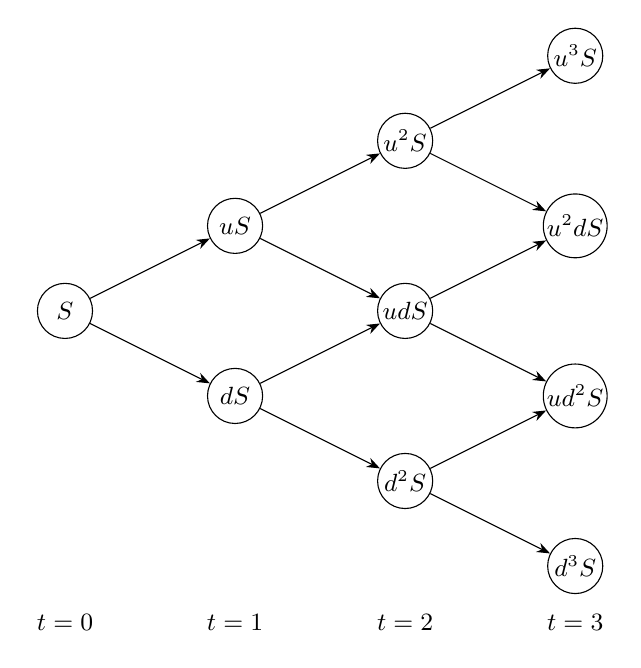
\begin{tikzpicture}[scale=0.9,
  nd/.style={draw, circle, minimum size=7mm, inner sep=0.5pt, font=\small}]
\node[nd] (S) at (0,0) {$S$};
\node[nd] (u1) at (2.4,1.2) {$uS$};
\node[nd] (d1) at (2.4,-1.2) {$dS$};
\node[nd] (u2) at (4.8,2.4) {$u^2S$};
\node[nd] (m2) at (4.8,0) {$udS$};
\node[nd] (d2) at (4.8,-2.4) {$d^2S$};
\node[nd] (u3) at (7.2,3.6) {$u^3S$};
\node[nd] (a3) at (7.2,1.2) {$u^2dS$};
\node[nd] (b3) at (7.2,-1.2) {$ud^2S$};
\node[nd] (d3) at (7.2,-3.6) {$d^3S$};
\foreach \a/\b in {S/u1, S/d1, u1/u2, u1/m2, d1/m2, d1/d2,
  u2/u3, u2/a3, m2/a3, m2/b3, d2/b3, d2/d3}{
  \draw[-{Stealth}] (\a) -- (\b);}
\node at (0,-4.4) {\small $t=0$};
\node at (2.4,-4.4) {\small $t=1$};
\node at (4.8,-4.4) {\small $t=2$};
\node at (7.2,-4.4) {\small $t=3$};
\end{tikzpicture}
\caption{多期間二項モデル(3期間の例).各枝の上向きの遷移確率が $p$,
下向きが $1-p$ である.}
\label{fig:binomial-tree}
\end{figure}

\subsection{二期間二項モデル}

まず二期間の場合を考える($t=2$ が満期).原資産のツリーと同じノード上に,
対応する時点・状態における金融商品の価格・キャッシュフローを表すツリーを考える.
満期では,各ノードごとにペイオフが確定している.コールオプションでは,満期の
ペイオフは上から順に $\max(u^2S-K,0)$, $\max(udS-K,0)$, $\max(d^2S-K,0)$ で
ある.

\paragraph{$t=1$ の上昇ノードにおける評価.}
$t=1$ で原資産価格 $uS$ のノード上の複製ポートフォリオを求める.無リスク資産の
利回りを $r$,現在価格は1とする.コールオプションを原資産 $\Delta$ 単位,
無リスク資産 $B$ 単位で複製できたとすると,無裁定条件より次の式が成り立つ:
\begin{align}
\Delta\,u^2S + B(1+r) &= \max(u^2S-K,\,0) \equiv P(uu),\notag\\
\Delta\,udS + B(1+r) &= \max(udS-K,\,0) \equiv P(ud).
\end{align}
この連立方程式を解くと,
\begin{equation}
\Delta = \frac{1}{uS}\,\frac{P(uu)-P(ud)}{u-d},\qquad
B = \frac{1}{1+r}\,\frac{u\,P(ud) - d\,P(uu)}{u-d}
\end{equation}
となり,複製ポートフォリオが得られた.一期間モデルと比較すると,$\Delta$ の
分母の「原資産価格の違い」と分子の「CFの違い」が,このノードのものに変わって
いるだけである.

コールオプションの $t=1$ の上昇ノードにおける価値は,
\begin{align}
C_u = uS\times\Delta + 1\times B
&= \frac{P(uu)-P(ud)}{u-d} + \frac{1}{1+r}\,\frac{uP(ud)-dP(uu)}{u-d}\notag\\
&= \frac{(1+r-d)\,P(uu) - (1+r-u)\,P(ud)}{(u-d)(1+r)}
\end{align}
であり,この価格は次のように書ける:
\begin{equation}
C_u = \frac{\dfrac{1+r-d}{u-d}P(uu)
+ \Bigl(1 - \dfrac{1+r-d}{u-d}\Bigr)P(ud)}{1+r}.
\end{equation}
分子は,$q = (1+r-d)/(u-d)$ を上昇確率としたときの,コールオプションの
(このノードから見た)次期のペイオフの期待値に相当し,分母は無リスク資産の
利回りによる割引に相当する.

\paragraph{$t=1$ の下落ノードと $t=0$ の評価.}
$t=1$ の下落ノードにおける価値 $C_d$ も同様に得られる.さらに $t=0$ における
現在価値を考える.$t=1$ の値 $C_u$, $C_d$ を「満期1期のペイオフ」とみなして,
同じ複製の議論を行う.コールオプションを原資産 $\Delta$ 単位,無リスク資産
$B$ 単位で複製できたとすると,
\begin{align}
\Delta\,uS + B(1+r) &= C_u,\notag\\
\Delta\,dS + B(1+r) &= C_d
\end{align}
より
\begin{equation}
\Delta = \frac{1}{S}\,\frac{C_u - C_d}{u-d},\qquad
B = \frac{1}{1+r}\,\frac{uC_d - dC_u}{u-d}
\end{equation}
となる(複製ポートフォリオが得られた).

\paragraph{$t=0$ の価値.}
コールオプションの $t=0$ のノードにおける価値は,$q = \dfrac{1+r-d}{u-d}$ と
おくと,
\begin{align}
C_0 = \Delta S + B
&= \frac{(1+r-d)C_u - (1+r-u)C_d}{(u-d)(1+r)}
= \frac{q\,C_u + (1-q)\,C_d}{1+r}\notag\\
&= \frac{1}{1+r}\Biggl[
q\,\frac{qP(uu) + (1-q)P(ud)}{1+r}
+ (1-q)\,\frac{qP(ud) + (1-q)P(dd)}{1+r}\Biggr]\notag\\
&= \frac{q^2P(uu) + 2q(1-q)P(ud) + (1-q)^2P(dd)}{(1+r)^2}.
\label{eq:two-period}
\end{align}
分子は確率 $q$ による満期ペイオフの期待値,分母は現在時点までの2期間分の割引で
ある.すなわち,
\begin{equation}
C_0 = \frac{\E^Q[C_2]}{(1+r)^2}
\end{equation}
が成り立つ.ただし $C_2$ はコールオプションの $t=2$ におけるペイオフ,
$\E^Q[\cdot]$ はリスク中立確率 $q$ による期待値である.

\subsection{一般の $n$ 期間への拡張}

前項の結論は次のように一般化できる:
\begin{equation}
C_0 = \frac{\E^Q[C_n]}{(1+r)^n}.
\label{eq:crr-general-call}
\end{equation}
ただし $C_n$ はコールオプションの $t=n$ におけるペイオフである.この式は,
コールに限らず,\textbf{一般の証券に関しても成り立つ}.$t=n$ のペイオフ関数を
原資産価格の関数 $f(S_n)$ とすると,$t=0$ における現在価値 $V_0$ は
\begin{equation}
V_0 = \frac{\E^Q[f(S_n)]}{(1+r)^n}
= \frac{1}{(1+r)^n}\sum_{k=0}^{n}
{}_n\mathrm{C}_k\,q^k(1-q)^{n-k}\,f(u^k d^{n-k}S),
\qquad q = \frac{1+r-d}{u-d}
\label{eq:crr-general}
\end{equation}
で与えられる.ここで ${}_n\mathrm{C}_k\,q^k(1-q)^{n-k}$ は「上昇 $k$ 回,下落
$n-k$ 回のノードに達する確率」である.

\subsection{CRRの公式(コール・オプション)}

再度,コールオプションを考える.ペイオフは
$f(u^kd^{n-k}S) = \max(u^kd^{n-k}S - K,\,0)$ である.ここで,
\begin{quote}
$a$:満期でペイオフ関数が正の値をとるノードのうち,原資産価格が最低のノードを
示す $k$ の値(このノードで,ペイオフがはじめて$+$になる)
\end{quote}
を定義する.$k\geq a$ のノードでは $\max(u^kd^{n-k}S-K,0) = u^kd^{n-k}S-K > 0$,
$k<a$ のノードではペイオフは0である.

このとき,
\begin{align}
V_0 &= \frac{\E^Q[\max(S_n - K,\,0)]}{(1+r)^n}
= \frac{1}{(1+r)^n}\sum_{k=0}^{n}{}_n\mathrm{C}_k\,q^k(1-q)^{n-k}
\max(u^kd^{n-k}S - K,\,0)\notag\\
&= \frac{1}{(1+r)^n}\sum_{k=a}^{n}{}_n\mathrm{C}_k\,q^k(1-q)^{n-k}
(u^kd^{n-k}S - K)\notag\\
&= S\sum_{k=a}^{n}{}_n\mathrm{C}_k\,
\Bigl(\frac{qu}{1+r}\Bigr)^k\Bigl(\frac{(1-q)d}{1+r}\Bigr)^{n-k}
- \frac{K}{(1+r)^n}\sum_{k=a}^{n}{}_n\mathrm{C}_k\,q^k(1-q)^{n-k}.
\label{eq:crr-derivation}
\end{align}

ここで
\begin{equation}
q^* \equiv \frac{qu}{1+r}
\end{equation}
とおくと,
\begin{equation}
1 - q^* = \frac{1+r - qu}{1+r}
= \frac{(1+r)(u-d) - (1+r-d)u}{(u-d)(1+r)}
= \frac{d\,(u - 1 - r)}{(u-d)(1+r)}
= \frac{(1-q)\,d}{1+r}
\end{equation}
が成り立つ(すなわち $q^*$ も確率とみなせる).なお,
\[
q = \frac{1+r-d}{u-d}
\;\Longleftrightarrow\;
qu + (1-q)d = 1+r
\;\Longleftrightarrow\;
\frac{qu}{1+r} + \frac{(1-q)d}{1+r} = 1
\]
であり,真ん中の式は「(確率 $q$ のもとで)原資産の期待収益率 $= r$」,つまり
\textbf{リスク中立確率を使っている}という意味である.

さらに,二項モデルの\textbf{補分布関数}(離散分布における生存関数)
\begin{equation}
\phi(a; n, p) \equiv \sum_{k=a}^{n}{}_n\mathrm{C}_k\,p^k(1-p)^{n-k}
\end{equation}
を定義する.すると,\eqref{eq:crr-derivation}から
\begin{equation}
\boxed{\;
V_0 = S\,\phi(a; n, q^*) - \frac{K}{(1+r)^n}\,\phi(a; n, q)
\;}
\label{eq:crr-call}
\end{equation}
が得られる.ただし,$a$ は $u^ad^{n-a}S > K$ を満たす最小の整数であり,
\begin{equation}
\Bigl(\frac{u}{d}\Bigr)^a > \frac{K}{d^nS}
\;\Longleftrightarrow\;
a\log\frac{u}{d} > \log\frac{K}{d^nS}
\qquad\therefore\quad
a > \frac{\log(K/S) - n\log d}{\log(u/d)}
\label{eq:crr-a}
\end{equation}
を満たす最小の整数が $a$ である.

\subsection{CRRの公式(プット・オプション)}

同じ多期間二項モデルで,ヨーロピアン・プット・オプションの価格式(CRRの公式の
プットオプション版)を求める.以下,コールオプションの価格式導出と対応させて
書く(講義では自習箇所とされた).

一般化された結果
\begin{equation}
P_0 = \frac{\E^Q[P_n]}{(1+r)^n},\qquad
V_0 = \frac{\E^Q[f(S_n)]}{(1+r)^n}
= \frac{1}{(1+r)^n}\sum_{k=0}^{n}{}_n\mathrm{C}_k q^k(1-q)^{n-k}f(u^kd^{n-k}S)
\end{equation}
を使う($P_n$ はプットオプションの $t=n$ におけるペイオフ).ペイオフ関数は
$f(u^kd^{n-k}S) = \max(K - u^kd^{n-k}S,\,0)$ であり,プットのペイオフが正になる
のは $k \leq a-1$ のノード($a$ はコールと同じ,$u^ad^{n-a}S>K$ を満たす最小の
整数)である.このとき,
\begin{align}
V_0 &= \frac{\E^Q[\max(K-S_n,\,0)]}{(1+r)^n}
= \frac{1}{(1+r)^n}\sum_{k=0}^{a-1}{}_n\mathrm{C}_k\,q^k(1-q)^{n-k}
(K - u^kd^{n-k}S)\notag\\
&= \frac{K}{(1+r)^n}\sum_{k=0}^{a-1}{}_n\mathrm{C}_k\,q^k(1-q)^{n-k}
- S\sum_{k=0}^{a-1}{}_n\mathrm{C}_k\,
\Bigl(\frac{qu}{1+r}\Bigr)^k\Bigl(\frac{(1-q)d}{1+r}\Bigr)^{n-k}.
\end{align}
ここで,離散分布における分布関数
\begin{equation}
F(a; n, p) \equiv \sum_{k=0}^{a-1}{}_n\mathrm{C}_k\,p^k(1-p)^{n-k}
= 1 - \phi(a; n, p)
\end{equation}
を定義すると,
\begin{equation}
\boxed{\;
P_0 = \frac{K}{(1+r)^n}\,F(a; n, q) - S\,F(a; n, q^*)
\;}
\label{eq:crr-put}
\end{equation}
が得られる.

\begin{definition}[CRRモデルとCRRの公式]
ここまでで示してきた,多期間二項モデルによるオプションの価格付けモデルを
\textbf{CRRモデル}(Cox-Ross-Rubinsteinモデル)という.特に,彼らが導出した
ヨーロピアン・コール(プット)・オプション価格式\eqref{eq:crr-call},
\eqref{eq:crr-put}を \textbf{CRRの公式}(Cox-Ross-Rubinsteinの公式)という.
オプション価格の一般式\eqref{eq:crr-general}もCRRの公式と呼ぶことがある
(どこまでを「CRRの公式」と呼ぶかは明確でない).
\end{definition}

\section{補足:CRR公式の正確な表現(重要!)}

金利による割引の表現に注意が必要である.これまでは一期間の利子率を $r$ として
表示してきたが,本来,一期間を $\Delta t$ 年,満期を $n\Delta t$ 年,金利を
\emph{年率} $r$ として,
\begin{equation}
C_0 = \frac{\E^Q[C_n]}{(1+r\Delta t)^n}
\end{equation}
が正確な表現である(これまでの $r$ を $r\Delta t$ に置換する).同様にして,
一般化されたCRRの価格式は
\begin{equation}
V_0 = \frac{\E^Q[f(S_n)]}{(1+r\Delta t)^n}
= \frac{1}{(1+r\Delta t)^n}\sum_{k=0}^{n}
{}_n\mathrm{C}_k\,q^k(1-q)^{n-k}f(u^kd^{n-k}S),
\qquad
q = \frac{1 + r\Delta t - d}{u - d}
\end{equation}
が正確な表現である.

\paragraph{割引金利が一定でない場合.}
さらに,第 $i$ 期目($t_{i-1}$ から $t_i$ まで)の無リスク金利が確定的で,
年率 $r_i$ で与えられる(時点によって異なる)場合は,
\begin{equation}
C_0 = \frac{\E^Q[C_n]}{\prod_{i=1}^{n}(1 + r_i\Delta t)}
\end{equation}
になる.\emph{しかし},CRRの価格式は
\[
V_0 = \frac{\E^Q[f(S_n)]}{\prod_{i=1}^n(1+r_i\Delta t)}
= \frac{1}{\prod_{i=1}^n(1+r_i\Delta t)}
\sum_{k=0}^{n}{}_n\mathrm{C}_k\,q^k(1-q)^{n-k}f(u^kd^{n-k}S)
\]
とは\textbf{ならない}.一般に,確率 $q$ が無リスク金利 $r_i$ に依存して変わる
ため,確率分布を二項分布では表現できなくなるからである.

\section{プット・コール・パリティ}

\subsection{プットとコールのペイオフの関係}

コール・ロングとプット・ロングのペイオフを比べると,原資産,満期,行使価格が
等しいならば,
\[
\text{コール・ロングのペイオフ} - \text{プット・ロングのペイオフ}
= \text{原資産価格} - K,
\]
すなわち
\begin{equation}
\max(S(T)-K,\,0) - \max(K-S(T),\,0) = S(T) - K
\label{eq:payoff-identity}
\end{equation}
が成り立つ(もともとこれは恒等式である.$S(T)\geq K$ の場合と $S(T)<K$ の場合に
分けて確かめればよい).

\subsection{プットオプションの複製}

式\eqref{eq:payoff-identity}を変形した
\begin{equation}
\max(K - S(T),\,0) = \max(S(T)-K,\,0) - S(T) + K
\end{equation}
の左辺をプットのペイオフ,右辺を複製ポートフォリオのペイオフとみると,
「プットを1単位ロング」の複製ポートフォリオが
\begin{itemize}
\item[A.] コールを1単位ロング,
\item[B.] 原資産を1単位ショート,
\item[C.] 満期 $T$ の割引債を $K$ 単位ロング,
\end{itemize}
であることを示している.Cで,将来のキャッシュを「割引債」のロング(ケースに
よってはショート)で表現している点に注意する.

\subsection{プット・コール・パリティ}

無裁定の議論より,「オプションとその複製ポートフォリオは,現時点でも価格は
等しい」ので,次式が成り立つ.

\begin{theorem}[プット・コール・パリティ]
\begin{equation}
p(t) = c(t) - S(t) + K\,v(t,T),
\label{eq:put-call-parity}
\end{equation}
あるいは書き直して
\begin{equation}
p(t) + S(t) = c(t) + K\,v(t,T).
\end{equation}
ここで,$p(t)$:時刻 $t$ におけるヨーロピアンプットオプションの価格,
$c(t)$:時刻 $t$ におけるヨーロピアンコールオプションの価格,
$S(t)$:時刻 $t$ における原資産価格,
$v(t,T)$:時刻 $t$ における満期 $T$ の(無リスクな)割引債価格である.
\end{theorem}

この関係式を\textbf{プット・コール・パリティ}という.これは価格付けモデルに
依存しない,一般に成り立つ関係式である.コール価格が得られれば,プット価格は
この式から得られる.逆も同様である.

\section*{付録:信用リスクの評価(参考)}

二項モデルによる信用リスクの評価を紹介する(講義では扱わない参考資料である).

\paragraph{信用リスクとは.}
\begin{itemize}
\item \textbf{デフォルト}:発行体や取引先が債務を履行できなくなる状態.
\item \textbf{信用リスク} (credit risk):デフォルトにより被る直接的・間接的な
損失.
  \begin{itemize}
  \item 直接的な損失:将来の契約が履行されなくなることによる損失.
  \item 間接的な損失:デフォルトの可能性の高まりにより,その証券の取引価格が
  下落すること.
  \end{itemize}
\end{itemize}

デフォルトによる直接的な損失の例として,クーポン3円・満期6年・額面100円の債券を
考えると,予定キャッシュフローは毎年3円+満期に103円だが,例えば4年目に
デフォルトが発生すると,極端な場合,デフォルト発生以降のキャッシュフローはゼロに
なる.

\paragraph{例:割引社債の二項モデル評価.}
一般事業会社Aが満期1年の割引社債を発行したとする.投資家は,デフォルトしなければ
1年後に1円受け取り,満期前にデフォルトしたら1年後に $\delta$ 円受け取ると仮定
する($0\leq\delta\leq 1$.$\delta$ は\textbf{回収率}と呼ばれる).

この割引社債の評価を二項モデルで考える.二項モデルの将来ノードは,ペイオフに
関連する状態を表していればよい.複数のノードでペイオフが等しくなってもよいし,
必ずしも原資産価格の水準の変化だけで考えなくてよい.柔軟に考えるほど,応用先は
広がる.

(リスク中立確率下の)デフォルト確率を $q$,デフォルト時の回収率を $\delta$ と
する.$t=1$ で,(1) 常に1円受け取る証券と,(2) デフォルト時のみ1円受け取る
証券を考える.(1) は無リスクな債券(割引債,現在価格 $1/(1+r)$),(2) は
CDS (Credit Default Swap) である.「デフォルト時にのみ1円受け取れる証券
(CDS)」が存在すれば,そのCDSと無リスク証券で社債を複製可能である.

無リスク金利 $r$ を一定とすると,リスク中立化法より,社債の現在価格は
\begin{equation}
\pi = \frac{\E^Q[C]}{1+r} = \frac{(1-q)\times 1 + q\times\delta}{1+r}.
\end{equation}
この式は
\begin{equation}
\pi = \frac{1}{1+r} - (1-\delta)\,\frac{q}{1+r}
\end{equation}
と書ける.第1式は「キャッシュフローの期待値の割引価値が現在価格になる」ことを
示し,第2式は複製ポートフォリオを示している:第1項は無リスクの割引債(これも
無リスク資産の一表現)を1単位ロング,第2項はCDSを $(1-\delta)$ 単位ショート,
である.

% ---------------- 演習問題 ----------------
\section{演習問題}

\begin{exercise}[問題11-1]
多期間二項モデルのCRRの公式で,プット・コール・パリティを確認しなさい.
\end{exercise}

\begin{answerbox}
\textbf{考え方.}CRRのプット価格式\eqref{eq:crr-put}に
$F(a;n,p) = 1-\phi(a;n,p)$ を代入し,プット・コール・パリティの右辺
$c - S + K(1+r\Delta t)^{-n}$ の形になることを計算で確かめる.

\medskip
\textbf{解答.}
一期間を $\Delta t$ 年とする正確な表現で書く.CRRの公式より
\begin{align*}
\mathrm{Put} + S - \frac{K}{(1+r\Delta t)^n}
&= \frac{K}{(1+r\Delta t)^n}F(a;n,q) - S\,F(a;n,q^*)
+ S - \frac{K}{(1+r\Delta t)^n}\\
&= \frac{K}{(1+r\Delta t)^n}\bigl(F(a;n,q) - 1\bigr)
+ S\bigl(1 - F(a;n,q^*)\bigr)\\
&= -\frac{K}{(1+r\Delta t)^n}\,\phi(a;n,q) + S\,\phi(a;n,q^*)\\
&= \mathrm{Call}.
\end{align*}
すなわち
\[
\mathrm{Put} = \mathrm{Call} - S + \frac{K}{(1+r\Delta t)^n}
\]
が成り立つ.右辺の第3項 $K(1+r\Delta t)^{-n}$ は満期 $n\Delta t$ の割引債
$K$ 単位の現在価値 $K\,v(0,T)$ にほかならないから,これはプット・コール・
パリティ\eqref{eq:put-call-parity}そのものである.$\blacksquare$

\medskip
\textbf{ポイント.}CRRの公式は特定のモデル(二項モデル)による価格式だが,
そこから得られるコール価格とプット価格は,モデルフリーな関係式である
プット・コール・パリティをきちんと満たしている.価格モデルの整合性チェックの
好例である.
\end{answerbox}

\begin{exercise}[問題11-2]
ここで説明した多期間二項モデルを使い,満期 $T$,バリアー価格 $B$ で $A$ 円を
受け取るデジタル・オプションの価格式を求めなさい.

デジタル・オプションとは,満期 $T$ における原資産価格 $S(T)$ がバリアー価格
$B$ を上回るとき,満期 $T$ に一定額 $A$ 円を受け取る証券である.$S(T)<B$ の
ときは何も受け取れない.
\end{exercise}

\begin{answerbox}
\textbf{考え方.}CRRの一般式\eqref{eq:crr-general}に,デジタル・オプションの
ペイオフ関数を代入すればよい.ペイオフはノードの原資産価格が $B$ を上回るか
どうかだけで決まるので,和はペイオフが正になるノードだけに絞られる.

\medskip
\textbf{解答.}
満期 $T$ におけるキャッシュフローは
$f(S(T)) = A\,\bm{1}_{\{S(T)>B\}}$ なので,CRRの公式より
\begin{align*}
V_0 &= \frac{\E^Q[f(S_n)]}{(1+r\Delta t)^n}
= \frac{1}{(1+r\Delta t)^n}\sum_{k=0}^{n}
{}_n\mathrm{C}_k\,q^k(1-q)^{n-k}\,A\times\bm{1}_{\{u^kd^{n-k}S > B\}}\\
&= \frac{A}{(1+r\Delta t)^n}\sum_{k=b}^{n}{}_n\mathrm{C}_k\,q^k(1-q)^{n-k}
= \frac{A}{(1+r\Delta t)^n}\,\phi(b;n,q).
\end{align*}
(注:$\bm{1}_A$ は定義関数で,事象 $A$ が真のとき1,偽のとき0.)
ただし,$b$ は $u^bd^{n-b}S > B$ を満たす最小の整数で,
\[
\Bigl(\frac{u}{d}\Bigr)^b > \frac{B}{d^nS}
\;\Longleftrightarrow\;
b\log\frac{u}{d} > \log\frac{B}{d^nS}
\qquad\therefore\quad
b > \frac{\log(B/S) - n\log d}{\log(u/d)}.
\]
($B\to K$ とみなすと,$b$ はこれまで使ってきた $a$ と同じである.)

\medskip
\textbf{ポイント.}コールオプションの価格式\eqref{eq:crr-call}の第2項
(行使価格の支払い部分)は,実は「$S(T)>K$ のとき $K$ 円支払う」デジタル・
オプションの価値である.デジタル・オプションはCRR公式の構成要素そのものと
言える.
\end{answerbox}

\begin{exercise}[問題11-3]
ここで説明したCRRモデルを用いて,
\begin{itemize}
\item 原資産価格 $S(0) = 100$ 円,
\item 満期1年,
\item 行使価格 $K = 100$ 円,
\item $\Delta t = 1/4$ 年($=$ 3ヶ月),
\item 無リスク金利 4\%(年率),
\item $u = 1.1$, $d = 0.9$
\end{itemize}
のときのヨーロピアン・コール・オプションの価格を求めなさい.
\end{exercise}

\begin{answerbox}
\textbf{考え方.}$n = 1/\Delta t \times 1$年 $= 4$ 期間の二項モデルである.
CRRの公式(正確な表現)を使うため,(1) リスク中立確率 $q$,(2) $q^*$,
(3) ペイオフが正になる最小ノード $a$,を順に計算し,公式\eqref{eq:crr-call}に
代入する.

\medskip
\textbf{解答.}
まず,原資産価格のリスク中立的な上昇確率は
\[
q = \frac{1 + r\Delta t - d}{u - d}
= \frac{1 + 0.04\times 0.25 - 0.9}{1.1 - 0.9} = \frac{0.11}{0.2} = 0.55
\]
より,55\%である.さらに,
\[
q^* = \frac{qu}{1+r\Delta t} = \frac{0.55\times 1.1}{1 + 0.04\times 0.25}
= \frac{0.605}{1.01} = 0.59901\ldots.
\]
次に,ペイオフが正になるノードを示す $k=a$ は,
\[
a > \frac{\log(K/S) - n\log d}{\log(u/d)}
= \frac{\log(100/100) - 4\log 0.9}{\log(1.1/0.9)} = 2.100\ldots
\]
より,$a = 3$ である.

CRRの公式より,コール・オプション価格は
\begin{align*}
V_0 &= S\,\phi(a;n,q^*) - \frac{K}{(1+r\Delta t)^n}\,\phi(a;n,q)\\
&= 100\,\phi(3;4,\ 0.59901) - \frac{100}{(1+0.04\times 0.25)^4}\,
\phi(3;4,\ 0.55)\\
&= 100\times 0.473490 - \frac{100}{1.01^4}\times 0.390981\\
&\approx 9.7765 \text{ 円}.
\end{align*}
ここで
\[
\phi(3;4,q^*) = {}_4\mathrm{C}_3\,(q^*)^3(1-q^*) + (q^*)^4 = 0.473490,
\qquad
\phi(3;4,q) = {}_4\mathrm{C}_3\,q^3(1-q) + q^4 = 0.390981
\]
である.

\medskip
\textbf{検算(4期間二項ツリーによる後ろ向き帰納法).}
満期のペイオフは,上から
$u^4S - K = 46.41$,\ $u^3dS - K = 19.79$,\ 0,\ 0,\ 0 であり,各ノードで
$V = [qV_u + (1-q)V_d]/(1+r\Delta t)$ を繰り返すと,
\[
t=3:\ (34.0901,\ 10.77673,\ 0,\ 0),\quad
t=2:\ (23.36543,\ 5.868518,\ 0),\quad
t=1:\ (15.33844,\ 3.195728)
\]
を経て $t=0$ で $9.776452$ 円となり,CRRの公式による値と一致する.
\end{answerbox}

% 第12章 ブラック・ショールズ・モデル(資料12 + BS公式導出補足)
\chapter{ブラック・ショールズ・モデル}

最終章では，連続時間モデルによるデリバティブの価格付け，すなわち
\textbf{ブラック・ショールズ(BS)モデル}を学ぶ。離散時間の二項モデル(CRR)から
連続時間モデルへ移行し，ヨーロピアン・オプションの解析的な価格公式
(Black-Scholesの公式)を導出する。また，デリバティブのリスク管理に使われる
\textbf{グリークス} (Greeks) と，通貨・金利デリバティブへの応用の考え方を扱う。

\section{ブラック・ショールズ(BS)モデル}

\subsection{前提}

\begin{itemize}
\item 完全市場(第9章参照)を仮定する。
\item 安全資産の利回り $r$($=$無リスク金利)は期間を通して一定とする。
\end{itemize}
さらに，簡単化のために以下を仮定する(これらの仮定は緩和可能である)。
\begin{itemize}
\item 市場には，1つのリスク性資産($=$原資産)と無リスク資産だけが存在する
(ということは，複製はこれら2資産を使って考える)。
\item リスク性資産に配当はない。
\end{itemize}
以下では，\textbf{リスク中立確率のもとで}，連続時間モデルで考える(連続時間
なので，ほんの一瞬の間の変化を考える)。

\subsection{モデルの定式化}

Black-Scholes(-Merton) モデルでは，微小時間 $\Delta t$ における瞬間的な収益率が，
\[
\text{期待値 } r\Delta t \quad
(\text{リスク中立確率下の議論なので } r \neq \mu),\qquad
\text{分散 } \sigma^2\Delta t
\]
の正規分布に従う，と仮定する。$\Delta$ で増分を表すと，
\[
\frac{\Delta S(t)}{S(t)} \sim N(r\Delta t,\ \sigma^2\Delta t),
\qquad \Delta S(t) = S(t+\Delta t) - S(t).
\]
無限小時間 $dt$ における式として表現すると，
\[
\frac{\dd S(t)}{S(t)} \sim N(r\,\dd t,\ \sigma^2\dd t),
\qquad \dd S(t) = S(t+\dd t) - S(t).
\]
しかも，瞬間的な収益率は時系列的に独立と仮定する。

これを，以下のように表現する：
\begin{equation}
\frac{\dd S(t)}{S(t)} = r\,\dd t + \sigma\,\dd W(t).
\label{eq:bs-sde}
\end{equation}
\begin{itemize}
\item 左辺は，無限小時間 $dt$ における瞬間的な収益率を表す。
\item 右辺第1項は，期待収益率 $r$ による $dt$ 間の増分を表す。
\item 右辺第2項は，$dt$ 間の収益率の確率的な増分(変動)を表す。変動の大きさは
$\sigma$ で調整する。
\end{itemize}

\begin{definition}[標準ブラウン運動]
$W(t)$ は\textbf{標準ブラウン運動}と呼ばれている確率過程で，次の性質をもつ。
\begin{itemize}
\item $\dd W(t) = W(t+\dd t) - W(t)$：標準ブラウン運動の無限小増分。
\item 無限小増分 $\dd W(t)$ は正規分布 $N(0,\,\dd t)$ に従う
($\Rightarrow \E[\dd W(t)] = 0$)。
\item 互いに背反な時間区間の無限小増分は，独立。
\item $W(0) = 0$， a.s.
\end{itemize}
\end{definition}

\begin{example}[問1]
式\eqref{eq:bs-sde}が $\dd S(t)/S(t) \sim N(r\,\dd t, \sigma^2\dd t)$ を満たす
ことを確認せよ。

\textbf{解。}(1) 期待値と分散を計算する：
\[
\E\Bigl[\frac{\dd S(t)}{S(t)}\Bigr] = r\,\dd t + \sigma\E[\dd W(t)] = r\,\dd t,
\qquad
\Var\Bigl[\frac{\dd S(t)}{S(t)}\Bigr] = \sigma^2\Var[\dd W(t)] = \sigma^2\dd t.
\]
(2) 右辺 $r\,\dd t + \sigma\,\dd W(t)$ は，正規分布に従う確率変数
$\dd W(t)$ の1次式なので正規分布に従う。よって
$\dd S(t)/S(t) \sim N(r\,\dd t, \sigma^2\dd t)$ である。
\end{example}

\begin{example}[問2]
では，$W(t)$ はどのような分布に従うか?

\textbf{解。}(1)
\[
W(t) = \int_0^t \dd W(s)
= \lim_{n\to\infty}\sum_{i=1}^{n}
\Bigl[W\Bigl(\frac{it}{n}\Bigr) - W\Bigl(\frac{(i-1)t}{n}\Bigr)\Bigr]
\]
と表現して，互いに背反な時間区間の増分の和に分解する。各増分は独立に
$N(0, t/n)$ に従う。(2) 正規分布の再生性(独立な正規変数の和は正規分布)を
使うと，$W(t) \sim N(0,\,t)$ が得られる。
\end{example}

\vspace{18pt}

\subsection{単純な積分ではうまくいかない}

式\eqref{eq:bs-sde}はリスク性資産価格の\emph{瞬間的な増分}の分布を示す式で
あって，将来時点 $t$ の価格 $S(t)$ の分布を示してはいない。単純に積分しても
有益な情報は出てこない：
\[
\dd S(t) = rS(t)\,\dd t + \sigma S(t)\,\dd W(t)
\]
\[
\int_0^T \dd S(t) = r\int_0^T S(t)\,\dd t + \sigma\int_0^T S(t)\,\dd W(t)
\]
\[
S(T) = S(0) + r\int_0^T S(t)\,\dd t + \sigma\int_0^T S(t)\,\dd W(t).
\]
被積分関数に確率過程 $S(t)$ が含まれたままなので，$S(T)$ の分布が上の式から
直接得られることはない。

そこで，算術収益率でなく，\textbf{対数収益率}で考えてみる(結果から言うと，
この方針をとるとうまくいく)。瞬間的な対数収益率は
$\dd\log S(t) = \log S(t+\dd t) - \log S(t)$ である。$\dd\log S(t)$ はどのような
分布に従うか。結果を先取りすると，$\dd\log S(t) \sim N(r\,\dd t, \sigma^2\dd t)$
には\emph{ならない}。やりたいことは，$f(t,S) = \log S$ の微小増分
$\dd f(t,S(t))$ を求めることである。このように，微小増分 $\dd S(t)$ の分布が
既知のとき，微小増分 $\dd f(t, S(t))$ の分布がどうなるかを考える時のツールが
\textbf{伊藤の公式}である。詳しく言うと，ある確率過程が与えられたとき，その
確率過程を含む汎関数(関数の関数)がどのように書けるか，を示す公式である。

\subsection{伊藤の公式}

$\dd S(t) = S(t)(r\,\dd t + \sigma\,\dd W(t))$ は既知とする。二変数関数
$f(t, S(t))$ を考え，無限小時間 $dt$ における微小増分 $\dd f(t,S(t))$ を考える。
2変数関数のテーラー展開を使うと，
\begin{equation}
\dd f(t,S(t)) = \frac{\partial f}{\partial t}\dd t
+ \frac{\partial f}{\partial S}\dd S(t)
+ \frac{1}{2}\frac{\partial^2 f}{\partial t^2}(\dd t)^2
+ \frac{\partial^2 f}{\partial t\,\partial S}\dd t\,\dd S(t)
+ \frac{1}{2}\frac{\partial^2 f}{\partial S^2}(\dd S(t))^2 + \cdots.
\end{equation}
ここで $\dd S(t) = S(t)(r\,\dd t + \sigma\,\dd W(t))$ を代入して整理すると，
\begin{align}
\dd f(t,S(t))
&= \frac{\partial f}{\partial t}\dd t
+ \frac{\partial f}{\partial S}S(t)\bigl(r\,\dd t + \sigma\,\dd W(t)\bigr)
+ \frac{1}{2}\frac{\partial^2 f}{\partial S^2}S(t)^2
\bigl(r\,\dd t + \sigma\,\dd W(t)\bigr)^2 + \cdots\notag\\
&= \Bigl(\frac{\partial f}{\partial t} + rS(t)\frac{\partial f}{\partial S}\Bigr)
\dd t + \sigma S(t)\frac{\partial f}{\partial S}\dd W(t)
+ \frac{1}{2}\sigma^2 S(t)^2\frac{\partial^2 f}{\partial S^2}(\dd W(t))^2
+ (\text{高次項}).
\end{align}
1次より高いオーダー($(\dd t)^2$， $\dd t\,\dd W(t)$ 等)を無視すると，最後に
$(\dd W(t))^2$ の項が残る。

\begin{keypoint}[$(\dd W(t))^2 = \dd t$：このページが肝心!]
重要：$\dd W(t)$ のオーダーは $(\dd t)^{0.5}$ である。実際，
\[
\Var[\dd W(t)] = \E\bigl[(\dd W(t) - \E[\dd W(t)])^2\bigr]
= \E[(\dd W(t))^2] = \dd t,
\]
であり，さらに($N(0,\dd t)$ の4次モーメント $3(\dd t)^2$ を使うと)
\begin{align*}
\Var[(\dd W(t))^2]
&= \E\bigl[((\dd W(t))^2 - \E[(\dd W(t))^2])^2\bigr]
= \E\bigl[((\dd W(t))^2 - \dd t)^2\bigr]\\
&= \E[(\dd W(t))^4] - 2\,\dd t\,\E[(\dd W(t))^2] + (\dd t)^2
= 3(\dd t)^2 - (\dd t)^2 = 2(\dd t)^2.
\end{align*}
よって $(\dd W(t))^2$ は平均 $\dd t$，分散 $2(\dd t)^2$ である。分散は $\dd t$ の
2次項なので無視すると，\textbf{$(\dd W(t))^2 = \dd t$ とみなせる}。
\end{keypoint}

上記を使い，$\dd t$ と $\dd W(t)$(一次)より高次の項を無視すると，
\begin{equation}
\dd f(t,S(t))
= \Bigl(\frac{\partial f}{\partial t} + rS(t)\frac{\partial f}{\partial S}
+ \frac{1}{2}\sigma^2S(t)^2\frac{\partial^2 f}{\partial S^2}\Bigr)\dd t
+ \sigma S(t)\frac{\partial f}{\partial S}\,\dd W(t).
\label{eq:ito}
\end{equation}
この式を\textbf{伊藤の公式}という。

\subsection{対数価格の確率微分方程式と $S(T)$ の分布}

$f(t,S(t)) = \log S(t)$ として伊藤の公式\eqref{eq:ito}を用いると，
$\partial f/\partial t = 0$， $\partial f/\partial S = 1/S$，
$\partial^2 f/\partial S^2 = -1/S^2$ より
\begin{equation}
\dd\log S(t)
= \Bigl(r - \frac{1}{2}\sigma^2\Bigr)\dd t + \sigma\,\dd W(t)
\label{eq:dlogS}
\end{equation}
となる。すなわち，
$\dd S(t)/S(t) = r\,\dd t + \sigma\,\dd W(t)$
($\dd S(t) = rS(t)\dd t + \sigma S(t)\dd W(t)$)と違い，
\eqref{eq:dlogS}は\textbf{右辺の $\dd t$ 項の係数と $\dd W(t)$ 項の係数が定数
(確定関数)}である。そのため，両辺を時間積分した結果が明確に書ける。

そこで，以後は Black-Scholesモデルとして
\begin{equation}
\dd\log S(t) = \Bigl(r - \frac{1}{2}\sigma^2\Bigr)\dd t + \sigma\,\dd W(t)
\end{equation}
を考える。両辺積分すると
\[
\log\frac{S(T)}{S(0)} = \Bigl(r - \frac{1}{2}\sigma^2\Bigr)T + \sigma W(T)
\]
となるので，
\begin{equation}
S(T) = S(0)\exp\Bigl\{\Bigl(r - \frac{1}{2}\sigma^2\Bigr)T + \sigma W(T)\Bigr\},
\qquad T \geq 0.
\label{eq:ST}
\end{equation}

\begin{keypoint}[BSモデルの特徴]
\begin{itemize}
\item $S(0) > 0$ ならば，常に $S(T) > 0$。
\item $\log S(T)$ は正規分布
$N\bigl(\log S(0) + (r-\sigma^2/2)T,\ \sigma^2 T\bigr)$ に従う。
$\Rightarrow$ $S(T)$ は\textbf{対数正規分布}に従う。
\end{itemize}
\end{keypoint}

\section{BSモデルによるオプション価格公式の導出}

\subsection{方針}

ヨーロピアン・コール・オプションとプット・オプションの価格式が，BSモデルでは
どのように表現されるかを導出したい。

(過去の資料の方針)手掛かりは，多期間二項モデルで得られたCRRの公式と，前述の
BSモデルに関する数式である。離散時間モデル(CRR)から連続時間モデル(BS)へ
移行する。そこで使うロジックは：満期を固定し，期間分割数を $n\to\infty$ とした
とき，多期間二項モデルがBSモデルに収束するようにパラメータを設定すれば，CRRの
公式はBSモデルの下でのオプション価格式に収束するはず，というものである。

(この資料の方針)せっかく\textbf{リスク中立化法}を学んだので，それを使用する。
すなわち，「リスク中立確率の下における将来キャッシュフローの割引現在価値の
期待値が，証券(デリバティブ)の現在の価格になる」ことを使う。

\subsection{連続時間モデルのリスク中立化法}

これを連続時間モデルで表現すると，金利 $r$ が一定のとき，
\begin{equation}
C_0 = \E^Q\bigl[e^{-rT}f(S(T))\bigr] = e^{-rT}\,\E^Q\bigl[f(S(T))\bigr].
\label{eq:rn-valuation}
\end{equation}
ここで，$T$：満期，$S(t)$：時刻 $t$ の原資産価格，$f(\cdot)$：デリバティブの
ペイオフ関数である。例えばヨーロピアンコールオプションでは
$f(S(T)) = \max(S(T)-K,\,0)$ である。

\subsection{コールの価格式の導出}

原資産価格 $S(t)$，満期 $T$，行使価格 $K$ のヨーロピアン・コール・オプションの
現在価値を求める。リスク中立化法を適用すると，
\begin{equation}
C_0 = e^{-rT}\E^Q[f(S(T))] = e^{-rT}\E^Q[\max(S(T)-K,\,0)].
\label{eq:call-rn}
\end{equation}
以後の式展開は，配布資料「Black-Scholesモデルによるヨーロピアン・コール・
オプション価格式」に基づく(以下，本節に全文を収録する)。

\paragraph{準備：$\log S(T)$ の密度関数。}
Black-Scholesモデルでは満期 $T$ の価格 $S(T)$ は，式\eqref{eq:ST}より
\[
S(T) = S\exp\Bigl\{\Bigl(r-\frac{\sigma^2}{2}\Bigr)T + \sigma Z^Q(T)\Bigr\}
\]
である。ただし $S = S(0)$，$Z^Q(t)$ は確率 $Q$ の下における標準ブラウン運動，
$r, \sigma$ は定数である。これより
\[
X(T) = \log S(T) = \log S + \Bigl(r-\frac{\sigma^2}{2}\Bigr)T + \sigma Z^Q(T)
\]
なので，$X(T)$ は平均
\[
\mu = \log S + \Bigl(r - \frac{\sigma^2}{2}\Bigr)T,
\]
分散 $\sigma^2 T$ の正規分布に従い，$X(T)$ の密度関数は
\begin{equation}
f_X(x) = \frac{1}{\sqrt{2\pi T}\,\sigma}\,
e^{-\frac{(x-\mu)^2}{2\sigma^2T}}
\end{equation}
である。そこで\eqref{eq:call-rn}を
\begin{align}
C_0 &= e^{-rT}\E^Q\bigl[\max(e^{X(T)} - K,\,0)\bigr]
= e^{-rT}\int_{-\infty}^{\infty}\max(e^x - K,\,0)\,f_X(x)\,\dd x
\end{align}
とすることにする。

\paragraph{積分領域の限定。}
この積分は $\max(\cdot,\cdot)$ を含むため，積分に寄与するのは
\[
\{x : \max(e^x - K, 0) > 0\} = \{x : e^x > K\} = \{x : x > \log K\}
\]
の領域だけである。よって
\begin{align}
C_0 &= e^{-rT}\int_{\log K}^{\infty}(e^x - K)\,
\frac{1}{\sqrt{2\pi T}\sigma}e^{-\frac{(x-\mu)^2}{2\sigma^2T}}\dd x
= e^{-rT}I_1 - Ke^{-rT}I_2,
\label{eq:c0-i1i2}
\end{align}
\begin{equation}
I_1 = \int_{\log K}^{\infty}e^x\,
\frac{1}{\sqrt{2\pi T}\sigma}e^{-\frac{(x-\mu)^2}{2\sigma^2T}}\dd x,
\qquad
I_2 = \int_{\log K}^{\infty}
\frac{1}{\sqrt{2\pi T}\sigma}e^{-\frac{(x-\mu)^2}{2\sigma^2T}}\dd x
\end{equation}
と書き直す。

\paragraph{$I_2$ の計算。}
変数変換
\[
y = \frac{x - \mu}{\sigma\sqrt{T}}
\]
をすると，
\begin{equation}
I_2 = \int_{\frac{\log K - \mu}{\sigma\sqrt{T}}}^{\infty}
\frac{1}{\sqrt{2\pi}}e^{-\frac{y^2}{2}}\dd y
= 1 - \Phi\Bigl(\frac{\log K - \mu}{\sigma\sqrt{T}}\Bigr)
= \Phi\Bigl(\frac{\mu - \log K}{\sigma\sqrt{T}}\Bigr).
\end{equation}
ただし，$\Phi(\cdot)$ は標準正規分布の分布関数である。

\paragraph{$I_1$ の計算。}
まず指数部を平方完成する：
\begin{align}
I_1 &= \int_{\log K}^{\infty}\frac{1}{\sqrt{2\pi T}\sigma}
e^{-\frac{(x-\mu)^2 - 2\sigma^2Tx}{2\sigma^2T}}\dd x
= \int_{\log K}^{\infty}\frac{1}{\sqrt{2\pi T}\sigma}
e^{-\frac{x^2 - 2(\mu+\sigma^2T)x + \mu^2}{2\sigma^2T}}\dd x\notag\\
&= \int_{\log K}^{\infty}\frac{1}{\sqrt{2\pi T}\sigma}
e^{-\frac{(x-(\mu+\sigma^2T))^2 + \mu^2 - (\mu+\sigma^2T)^2}{2\sigma^2T}}\dd x
= e^{\frac{(2\mu+\sigma^2T)\sigma^2T}{2\sigma^2T}}
\int_{\log K}^{\infty}\frac{1}{\sqrt{2\pi T}\sigma}
e^{-\frac{(x-(\mu+\sigma^2T))^2}{2\sigma^2T}}\dd x.
\end{align}
変数変換
\[
u = \frac{x - (\mu + \sigma^2 T)}{\sigma\sqrt{T}}
\]
を行うと，
\begin{align}
I_1 &= e^{\frac{2\mu+\sigma^2T}{2}}
\int_{\frac{\log K - (\mu+\sigma^2T)}{\sigma\sqrt{T}}}^{\infty}
\frac{1}{\sqrt{2\pi}}e^{-\frac{u^2}{2}}\dd u\notag\\
&= e^{\frac{2\mu+\sigma^2T}{2}}
\Bigl(1 - \Phi\Bigl(\frac{\log K - (\mu+\sigma^2T)}{\sigma\sqrt{T}}\Bigr)\Bigr)\notag\\
&= e^{\frac{2\mu+\sigma^2T}{2}}
\Phi\Bigl(\frac{\mu + \sigma^2T - \log K}{\sigma\sqrt{T}}\Bigr)
\end{align}
となる。このままでもよいが，$\mu$ をもとの変数で表すと，
\begin{align}
\frac{\mu - \log K}{\sigma\sqrt{T}}
&= \frac{\log\frac{S}{K} + \bigl(r - \frac{\sigma^2}{2}\bigr)T}{\sigma\sqrt{T}},\\
\frac{\mu + \sigma^2T - \log K}{\sigma\sqrt{T}}
&= \frac{\log\frac{S}{K} + \bigl(r + \frac{\sigma^2}{2}\bigr)T}{\sigma\sqrt{T}},\\
\frac{2\mu + \sigma^2 T}{2}
&= \frac{2\log S + 2\bigl(r-\frac{\sigma^2}{2}\bigr)T + \sigma^2T}{2}
= \log S + rT
\end{align}
となる。

\paragraph{Black-Scholesのコール価格式。}
以上を\eqref{eq:c0-i1i2}に代入すると，ヨーロピアン・コール・オプションの価格式
\begin{align}
C_0 &= S\,\Phi\Biggl(\frac{\log\frac{S}{K}
+ \bigl(r+\frac{\sigma^2}{2}\bigr)T}{\sigma\sqrt{T}}\Biggr)
- Ke^{-rT}\,\Phi\Biggl(\frac{\log\frac{S}{K}
+ \bigl(r-\frac{\sigma^2}{2}\bigr)T}{\sigma\sqrt{T}}\Biggr)\notag\\
&= S\,\Phi\Biggl(\frac{\log\frac{S}{K}
+ \bigl(r+\frac{\sigma^2}{2}\bigr)T}{\sigma\sqrt{T}}\Biggr)
- Ke^{-rT}\,\Phi\Biggl(\frac{\log\frac{S}{K}
+ \bigl(r+\frac{\sigma^2}{2}\bigr)T}{\sigma\sqrt{T}} - \sigma\sqrt{T}\Biggr)
\label{eq:bs-call}
\end{align}
が得られる。

\begin{remark}
式\eqref{eq:bs-call}の第2項の $\Phi(\cdot)$ は，リスク中立確率 $Q$ の下で満期
$T$ においてコールが行使される確率である。つまり，第2項は「行使時に支払う
行使価格の期待割引価値(行使確率を織り込んだもの)」を意味している。
\end{remark}

\vspace{18pt}

\subsection{Black-Scholesの公式}

\begin{keypoint}[Black-Scholesの公式]
\begin{align}
V_0^C &= S\,\Phi(a_1) - Ke^{-rT}\,\Phi\bigl(a_1 - \sigma\sqrt{T}\bigr),\notag\\
V_0^P &= Ke^{-rT}\,\Phi\bigl(-a_1+\sigma\sqrt{T}\bigr) - S\,\Phi(-a_1),\notag\\
a_1 &= \frac{\log(S/K) + (r + \sigma^2/2)\,T}{\sigma\sqrt{T}}.
\label{eq:bs-formula}
\end{align}
ここまでで求めた，連続時間モデルにおけるヨーロピアン・コール・
オプションおよびヨーロピアン・プット・オプションの価格式を，
\textbf{Black-Scholesの公式}(Black-Scholesのオプション価格式)という。
\end{keypoint}

\paragraph{プット価格式の導出。}
プット・コール・パリティ($r$ 一定なので $v(t,T) = e^{-r(T-t)}$ となることに
注意)より，プットオプションの価格は
\begin{align}
V_0^P &= V_0^C - S + Ke^{-rT}
= S\,\Phi(a_1) - Ke^{-rT}\Phi(a_1-\sigma\sqrt{T}) - S + Ke^{-rT}\notag\\
&= S\bigl(\Phi(a_1) - 1\bigr)
+ Ke^{-rT}\bigl(1 - \Phi(a_1-\sigma\sqrt{T})\bigr)\notag\\
&= Ke^{-rT}\,\Phi\bigl(-a_1 + \sigma\sqrt{T}\bigr) - S\,\Phi(-a_1)
\label{eq:bs-put}
\end{align}
となる。コール・オプションと同様の計算(省略)をしても導出できる。

\subsection{BS公式による複製ポートフォリオ}

\begin{itemize}
\item ヨーロピアン・コール・オプションの複製ポートフォリオ：「複製ポート
フォリオはリスク性資産 $\Delta$ 単位，(一単位あたり1円の)無リスク資産
$B$ 単位からなる」とすると，価格式\eqref{eq:bs-call}から
\begin{equation}
\Delta = \Phi(a_1),\qquad
B = -Ke^{-rT}\,\Phi\bigl(a_1 - \sigma\sqrt{T}\bigr).
\end{equation}
\item ヨーロピアン・プット・オプションの複製ポートフォリオ：同様に，価格式
\eqref{eq:bs-put}から
\begin{equation}
\Delta = -\Phi(-a_1),\qquad
B = Ke^{-rT}\,\Phi\bigl(-a_1 + \sigma\sqrt{T}\bigr).
\end{equation}
\end{itemize}

\subsection{本源的価値と時間価値}

コール価格のグラフ($K=100$， $r=0.1$， $\sigma=0.2$， $T=1$ の例)を原資産価格の
関数として描くと，満期のペイオフ $\max(S-K,0)$(これを\textbf{本源的価値}と
いう)より上に位置する滑らかな曲線になる。オプション価格と本源的価値の差を
\textbf{時間価値}という。

\begin{itemize}
\item ヨーロピアン\emph{コール}オプションでは，時間価値は正になることが多い。
\item しかし，ヨーロピアン\emph{プット}オプションでは，ITMが深い(原資産価格が
十分低い)領域で，オプション価格が本源的価値を\emph{下回る}(時間価値が負に
なる)ことがある。
\end{itemize}

\subsection{BS公式の振る舞い}

BS公式は多くの変数に依存するので，振る舞いは複雑である。ここでは
$V_0^C = V_0^C(S, K, T, \sigma, r)$ について，一つ一つの変数の動きと価格の
動きをみる(証明・確認は各自で考えること)。

\begin{itemize}
\item 原資産価格 $S$：
$S \to 0$ で $V_0^C \to 0$，\quad $S\to\infty$ で $V_0^C \to\infty$。
\item 行使価格 $K$：
$K \to 0$ で $V_0^C \to S$，\quad $K\to\infty$ で $V_0^C \to 0$。
\item 満期 $T$：
$T\to 0$ で $V_0^C \to \max(S-K, 0)$
($S\geq K$ なら $S-K$ へ，$S<K$ なら0へ)，\quad
$T\to\infty$ で $V_0^C \to S$。
\item ボラティリティ $\sigma$：
$\sigma\to 0$ で $V_0^C \to \max(S - Ke^{-rT},\,0)$
($S\geq Ke^{-rT}$ なら $S - Ke^{-rT}$ へ，$S<Ke^{-rT}$ なら0へ)，\quad
$\sigma\to\infty$ で $V_0^C \to S$。
\item 無リスク金利 $r$：
$r\to 0$ で $V_0^C \to V_0^C(S,K,T,\sigma,0)$，\quad
$r\to\infty$ で $V_0^C \to S$。
\end{itemize}

\begin{remark}[参考：デリバティブ価格の求め方]
デリバティブ価格の求め方には，
\begin{enumerate}
\item リスク中立化法を使い，(将来キャッシュフローの割引現在価値の)期待値を
解析的に計算する。
\item リスク中立化法を使い，期待値をモンテカルロ・シミュレーションで計算する。
\item 二項モデルのような格子モデルで，期待値を計算する。
\item 価格関数が満たす偏微分方程式を解き，価格を求める。
\end{enumerate}
などがある。本講義では1と3だけを扱った。
\end{remark}

\vspace{18pt}

\section{デリバティブのリスク管理：グリークス (Greeks)}

\subsection{リスクヘッジとリスク感応度}

\begin{itemize}
\item \textbf{リスク・ヘッジ}とは：ここでいうリスクとは，将来発生しうる価格の
変動性のこと。そのようなリスクを回避・低減することをリスク・ヘッジという。
\item \textbf{リスク感応度}：リスクの源泉となる変数が1単位動いたときの価格
(or 損失額)の変化量。(偏)微分係数で与えることもある(グリークスはこの
偏微分係数のこと)。変数の価格への影響度を示す。
\end{itemize}

\subsection{グリークス}

オプション価格 $V$ をテーラー展開すると($t$ は時刻，$T$ は満期までの期間で，
$\dd T = -\dd t$)，
\begin{align}
&V(S+\dd S,\ K,\ T-\dd t,\ \sigma+\dd\sigma,\ r+\dd r)\notag\\
&\quad = V(S,K,T,\sigma,r)
+ \frac{\partial V}{\partial S}\dd S
- \frac{\partial V}{\partial T}\dd t
+ \frac{\partial V}{\partial\sigma}\dd\sigma
+ \frac{\partial V}{\partial r}\dd r
+ \frac{1}{2}\frac{\partial^2V}{\partial S^2}(\dd S)^2 + \cdots.
\end{align}
これより，オプション価格の変化は幾つかの偏微分を使って表現できる。
これらのギリシャ文字で表現されるリスク指標を\textbf{グリークス}という。
\begin{itemize}
\item まずは一次の項を考える。実務では，デルタ・ヘッジ(後出)は当たり前の
ように実施する。
\item 実務では，ベガ・リスク(後出)と若干の高次のリスクにも着目する。
\item 二次の項で考慮するのは主にガンマ(後出)である。
\end{itemize}
以下ではヨーロピアン・コール・オプション
$V_0^C = V_0^C(S,K,T,\sigma,r)$ を中心に具体的な式を出す。

\subsection{デルタ($\Delta$)，ガンマ($\Gamma$)}

\begin{definition}[デルタ]
\textbf{デルタ} (Delta) は，原資産価格 $S$ が微小量変化したときの，オプション
価格の変化率である。オプション価格 $V$ の原資産価格 $S$ に関する偏微分で表現
される。ヨーロピアン・コールでは
\begin{equation}
\Delta = \frac{\partial V_0^C}{\partial S} = \Phi(a_1).
\end{equation}
\end{definition}

これは複製ポートフォリオにおける原資産の保有量 $\Delta = \Phi(a_1)$ と同じで
ある(「デルタ」の別の意味)。実際には，オプション価格 $V$ は原資産価格 $S$ の
非線形関数であり，$\Delta$ は $S$ に依存して時々刻々変化する。ということは，
\emph{複製ポートフォリオも時々刻々変化する}。

\begin{definition}[ガンマ]
$\Delta$ の $S$ への依存関係を示すのが\textbf{ガンマ} (Gamma) である：
\begin{equation}
\Gamma = \frac{\partial\Delta}{\partial S}
= \frac{\partial^2 V_0^C}{\partial S^2}
= \frac{1}{S\sigma\sqrt{T}}\,
\left.\frac{\dd\Phi(x)}{\dd x}\right|_{x=a_1}
= \frac{\varphi(a_1)}{S\sigma\sqrt{T}}
\end{equation}
($\varphi$ は標準正規密度関数)。
\end{definition}

$K=100$， $r=0.1$， $\sigma=0.2$， $T=1$ の例では，$\Delta$ は原資産価格とともに
0から1へS字型に増加し，$\Gamma$ はATM付近で最大となる山型になる。

\begin{keypoint}[ガンマとリバランス]
ガンマはリバランスのタイミングの目安の一つになる。
\begin{itemize}
\item ガンマが小さければ，原資産価格が少し変化してもデルタはあまり変化しない
$\to$ リバランスはやや間隔を空けても大丈夫…かも?
\item ガンマが大きければ，原資産価格が少し変化するだけでデルタはかなり変化する
$\to$ リバランスは頻繁に行うほうがよい…かも?
\end{itemize}
これらはリバランスに要するコストとの兼ね合いで決める。
\end{keypoint}

\subsection{セータ($\Theta$)}

\begin{definition}[セータ]
\textbf{セータ}(シータ，Theta)は，満期 $T$ が微小量変化したときのオプション
価格の変化率(満期を固定したオプションの価格の，瞬間的な変化率)である：
\begin{align}
\Theta &= \frac{\partial V_0^C}{\partial T}
= \frac{\sigma S}{2\sqrt{T}}\,\left.\frac{\dd\Phi(x)}{\dd x}\right|_{x=a_1}
+ rKe^{-rT}\,\Phi\bigl(a_1 - \sigma\sqrt{T}\bigr)\notag\\
&= \frac{\sigma S}{2\sqrt{T}}\varphi(a_1)
+ rKe^{-rT}\Phi(a_1-\sigma\sqrt{T}).
\end{align}
\end{definition}

\begin{itemize}
\item (コール)オプションでは $\Theta > 0$ になる(満期が長いほど価値が高い
から)。
\item 通常，$\Theta$ は満期付近では小さく，満期の少し手前で上昇し，その後は
満期から離れるほど低下する。ただし，アットザマネー近くの場合，満期直前まで
$\Theta$ は大きい値をとる($K=100$， $r=0.1$， $\sigma=0.2$ の例で，$S=98, 100,
102$ の3ケースの比較が講義で示された)。
\item 満期 $T$ の変化は確定的なので，あらかじめ予測可能・対処可能である。
\end{itemize}

\subsection{ロー($\rho$)，ベガ($\mathcal{V}$)}

\begin{itemize}
\item \textbf{ロー} (Rho)：金利 $r$ が微小量変化したときの，オプション価格の
変化率。
\begin{equation}
\rho = \frac{\partial V_0^C}{\partial r}.
\end{equation}
\item \textbf{ベガ} (Vega)：ボラティリティ $\sigma$ が微小量変化したときの，
オプション価格の変化率。
\begin{equation}
\nu = \frac{\partial V_0^C}{\partial\sigma}.
\end{equation}
\end{itemize}

vega risk は，市場では非常に注目されている(市場では，ボラティリティ $\sigma$ は
一定でないと認識されているからである)。vega の変化，特に vanna
($\partial\nu/\partial S$)と volga($\partial\nu/\partial\sigma$)も注目
されている。

\section{通貨・金利デリバティブへの応用}

\subsection{通貨デリバティブへの応用}

為替レートも確率変動するとみなして，Black-Scholesモデルを適用するという
考え方は，とてもわかりやすい。素朴には
\[
\frac{\dd X(t)}{X(t)} = r(t)\,\dd t + \sigma\,\dd W(t)\ ?
\]
としたくなるが，それぞれの国に無リスク金利があること，裁定機会の排除を考えると
(この講義の水準を越えるので詳細は略)，正しくは
\begin{equation}
\frac{\dd X(t)}{X(t)} = \bigl(r_d(t) - r_f(t)\bigr)\dd t + \sigma\,\dd W(t)
\end{equation}
となる。ここで，添字 $d$ は基準通貨，$f$ は別の通貨，$X(t)$ は基準通貨への
換算レート，$B_i(t)$ は $i$ 通貨の無リスク資産の時刻 $t$ における価値である。
こういったモデルを基準にして，考えていくことができる。

\subsection{金利デリバティブへの応用}

金利も確率変動するとみなして，Black-Scholesモデルを適用するという考え方は，
とてもわかりやすい。では，それは可能か(金利 $=$ 無リスク金利として考える)。

\begin{itemize}
\item 金利自体が市場取引される資産ではない。金利は利子・利息計算や割引計算で
使用される\emph{指標}に過ぎない。
\item 金利自体が利回り・収益率である。そのため，金利自身の(瞬間的な)期待
収益率が(無リスク)金利自身($\mu = r(t)$)とするのはおかしい。
$\to$ この表現はやや不適切。
\end{itemize}
考え方は少し複雑であり，この講義の水準を越えるので略す。

% ---------------- 演習問題 ----------------
\section{演習問題}

以下の演習問題について，解答例のPDFは配布資料に含まれていなかったため，
解答・解説は編集者が作成したものである。

\begin{exercise}[問題12-1]
Black-Scholesの公式でプット・コール・パリティを確認しなさい。
\end{exercise}

\begin{answerbox}
\textbf{考え方。}BSのコール価格式\eqref{eq:bs-call}とプット価格式
\eqref{eq:bs-put}の差を計算し，$\Phi(x) + \Phi(-x) = 1$ を使う。

\medskip
\textbf{解答。}$a_2 = a_1 - \sigma\sqrt{T}$ と書くと，
\begin{align*}
V_0^C - V_0^P
&= \bigl[S\Phi(a_1) - Ke^{-rT}\Phi(a_2)\bigr]
- \bigl[Ke^{-rT}\Phi(-a_2) - S\Phi(-a_1)\bigr]\\
&= S\bigl[\Phi(a_1) + \Phi(-a_1)\bigr]
- Ke^{-rT}\bigl[\Phi(a_2) + \Phi(-a_2)\bigr]\\
&= S - Ke^{-rT}.
\end{align*}
金利一定のもとで $v(0,T) = e^{-rT}$ なので，これは
\[
V_0^P = V_0^C - S + K\,v(0,T),
\]
すなわちプット・コール・パリティそのものである。$\blacksquare$
\end{answerbox}

\begin{exercise}[問題12-2]
Black-Scholesモデルにおけるヨーロピアン・プット・オプションの価格公式
$V_0^P = V_0^P(S,K,T,\sigma,r)$ の振る舞いを示しなさい。
\end{exercise}

\begin{answerbox}
\textbf{考え方。}プット・コール・パリティ $V_0^P = V_0^C - S + Ke^{-rT}$ を
使えば，本文で示したコールの振る舞いから，プットの振る舞いが直ちに得られる。

\medskip
\textbf{解答。}
\begin{itemize}
\item 原資産価格 $S$：$S\to 0$ で $V_0^C\to 0$ より
$V_0^P \to Ke^{-rT}$(確実に行使され，行使価格の現在価値になる)。
$S\to\infty$ では，$V_0^C - S \to 0$ となるので $V_0^P \to 0$。
\item 行使価格 $K$：$K\to 0$ で $V_0^P \to S - S = 0$。$K\to\infty$ で
$V_0^P \approx Ke^{-rT} - S \to \infty$。
\item 満期 $T$：$T\to 0$ で
$V_0^P \to \max(S-K,0) - S + K = \max(K-S,\,0)$(本源的価値に収束)。
$T\to\infty$ では $V_0^C\to S$，$Ke^{-rT}\to 0$($r>0$)より $V_0^P \to 0$。
\item ボラティリティ $\sigma$：$\sigma\to 0$ で
$V_0^P \to \max(S-Ke^{-rT},0) - S + Ke^{-rT} = \max(Ke^{-rT}-S,\,0)$。
$\sigma\to\infty$ で $V_0^C\to S$ より $V_0^P \to Ke^{-rT}$
(プットの価格上限)。
\item 無リスク金利 $r$：$r\to 0$ で $V_0^P \to V_0^P(S,K,T,\sigma,0)$。
$r\to\infty$ で $V_0^C\to S$，$Ke^{-rT}\to 0$ より $V_0^P\to 0$。
\end{itemize}

\medskip
\textbf{ポイント。}コールの価値は $S$ を上限として無限に増え得るのに対し，
プットの価値は $Ke^{-rT}$ が上限である(受け取れる金額が最大でも $K$ だから)。
また，満期を延ばすとコールは単調に価値が上がるが，プットは
「受取 $K$ の割引が進む」効果があるため，必ずしも単調ではない(これが
ヨーロピアン・プットの時間価値が負になり得ることと対応している)。
\end{answerbox}

\begin{exercise}[問題12-3]
ブラックショールズの公式のうち，ヨーロピアン・コール・オプションの価格式から，
グリークスを求めなさい。
(1) デルタ delta，(2) ガンマ gamma，(3) セータ theta，(4) ロー rho，
(5) ヴェガ vega(or ラムダ lambda)。
\end{exercise}

\begin{answerbox}
\textbf{考え方。}コール価格式
$V_0^C = S\Phi(a_1) - Ke^{-rT}\Phi(a_2)$，\ $a_2 = a_1 - \sigma\sqrt{T}$，
\[
a_1 = \frac{\log(S/K) + (r+\sigma^2/2)T}{\sigma\sqrt{T}}
\]
を各変数で偏微分する。計算を簡潔にする鍵は，標準正規密度
$\varphi(x) = \Phi'(x) = \frac{1}{\sqrt{2\pi}}e^{-x^2/2}$ に関する恒等式
\begin{equation}
S\,\varphi(a_1) = Ke^{-rT}\varphi(a_2)
\tag{$\ast$}
\end{equation}
である。($\ast$)は
$\varphi(a_2) = \varphi(a_1)e^{a_1\sigma\sqrt{T} - \sigma^2T/2}$ と
$e^{a_1\sigma\sqrt{T}} = (S/K)e^{(r+\sigma^2/2)T}$ を代入すれば確かめられる。

\medskip
\textbf{(1) デルタ。}$a_1, a_2$ の $S$ 依存性に注意して
\[
\Delta = \frac{\partial V_0^C}{\partial S}
= \Phi(a_1) + S\varphi(a_1)\frac{\partial a_1}{\partial S}
- Ke^{-rT}\varphi(a_2)\frac{\partial a_2}{\partial S}.
\]
$\partial a_1/\partial S = \partial a_2/\partial S = 1/(S\sigma\sqrt{T})$ と
($\ast$)より後ろの2項は相殺し，
\[
\boxed{\Delta = \Phi(a_1)}.
\]

\textbf{(2) ガンマ。}
\[
\Gamma = \frac{\partial\Delta}{\partial S}
= \varphi(a_1)\frac{\partial a_1}{\partial S}
= \boxed{\frac{\varphi(a_1)}{S\sigma\sqrt{T}}} > 0.
\]

\textbf{(3) セータ。}$T$ で偏微分する。
\[
\Theta = \frac{\partial V_0^C}{\partial T}
= S\varphi(a_1)\frac{\partial a_1}{\partial T}
+ rKe^{-rT}\Phi(a_2) - Ke^{-rT}\varphi(a_2)\frac{\partial a_2}{\partial T}.
\]
($\ast$)を使うと第1項と第3項は
$S\varphi(a_1)\bigl(\partial a_1/\partial T - \partial a_2/\partial T\bigr)$ に
まとまり，$a_1 - a_2 = \sigma\sqrt{T}$ より
$\partial(a_1-a_2)/\partial T = \sigma/(2\sqrt{T})$ なので，
\[
\boxed{\Theta = \frac{\sigma S}{2\sqrt{T}}\,\varphi(a_1)
+ rKe^{-rT}\,\Phi(a_2)} > 0.
\]
(本文のセータの式と一致する。)

\textbf{(4) ロー。}
\[
\rho = \frac{\partial V_0^C}{\partial r}
= S\varphi(a_1)\frac{\partial a_1}{\partial r}
+ KTe^{-rT}\Phi(a_2) - Ke^{-rT}\varphi(a_2)\frac{\partial a_2}{\partial r}.
\]
$\partial a_1/\partial r = \partial a_2/\partial r = \sqrt{T}/\sigma$ と($\ast$)
より第1項と第3項は相殺し，
\[
\boxed{\rho = KTe^{-rT}\,\Phi(a_2)} > 0.
\]

\textbf{(5) ベガ。}
\[
\nu = \frac{\partial V_0^C}{\partial\sigma}
= S\varphi(a_1)\frac{\partial a_1}{\partial\sigma}
- Ke^{-rT}\varphi(a_2)\frac{\partial a_2}{\partial\sigma}
= S\varphi(a_1)\Bigl(\frac{\partial a_1}{\partial\sigma}
- \frac{\partial a_2}{\partial\sigma}\Bigr)
\]
(2つ目の等号で($\ast$)を使用)。$a_1 - a_2 = \sigma\sqrt{T}$ より
$\partial(a_1-a_2)/\partial\sigma = \sqrt{T}$ なので，
\[
\boxed{\nu = S\sqrt{T}\,\varphi(a_1)} > 0.
\]

\medskip
\textbf{ポイント。}どの計算でも，恒等式($\ast$)によって「$a_1,a_2$ の中身の
微分から出てくる項」がすべて相殺される。結果として，デルタは行使確率に似た
$\Phi(a_1)$，ガンマとベガはATM付近で最大になる $\varphi(a_1)$ 型，ローと
セータの主要項は行使確率 $\Phi(a_2)$ 型，というきれいな構造になる。符号は
コールではすべて正である($\Theta>0$ は「満期までの期間 $T$ が長いほど価値が
高い」ことを表す)。
\end{answerbox}

\section*{講義のまとめにかえて}

本講義では，金融市場の基本(第1〜3章)，リスクと効用の考え方(第4章)，
現代ポートフォリオ理論(第5〜7章)，デリバティブとその価格付け(第8〜12章)を
学んだ。価格付けの中心にあるのは「無裁定」と「複製」，そしてそれらから導かれる
「リスク中立化法」である。講義の構成に挙げられていた「9. 金融リスク管理の基礎」
(リスク尺度，市場リスクと信用リスク，金融危機と金融規制)は，第4章の
VaR・ESへの言及，第8章のCDS，第11章付録の信用リスク評価で，その入口に触れて
いる。


\end{document}
